\newcommand{\NWtarget}[2]{\hypertarget{#1}{#2}}
\newcommand{\NWlink}[2]{\hyperlink{#1}{#2}}
\newcommand{\NWtxtMacroDefBy}{Fragment defined by}
\newcommand{\NWtxtMacroRefIn}{Fragment referenced in}
\newcommand{\NWtxtMacroNoRef}{Fragment never referenced}
\newcommand{\NWtxtDefBy}{Defined by}
\newcommand{\NWtxtRefIn}{Referenced in}
\newcommand{\NWtxtNoRef}{Not referenced}
\newcommand{\NWtxtFileDefBy}{File defined by}
\newcommand{\NWtxtIdentsUsed}{Uses:}
\newcommand{\NWtxtIdentsNotUsed}{Never used}
\newcommand{\NWtxtIdentsDefed}{Defines:}
\newcommand{\NWsep}{${\diamond}$}
\newcommand{\NWnotglobal}{(not defined globally)}
\newcommand{\NWuseHyperlinks}{}
\documentclass[11.5pt]{report}
\usepackage[a4paper, left=2cm, right=2cm, top=2cm]{geometry}
%\usepackage[text={16cm,24cm}]{geometry}
\usepackage{marginnote}


% https://stackoverflow.com/a/27243065/505306
% Making caption font smaller on figures and tables.
\usepackage{caption}
\captionsetup{font=footnotesize}

% Forcing line-breaks in url's
% https://tex.stackexchange.com/questions/3033/forcing-linebreaks-in-url
\usepackage[hyphens]{url}

%-------------------------------------------------------------------------------
%\usepackage[left,pagewise]{lineno}
%\linenumbers
\usepackage[framemethod=TikZ]{mdframed}
\usepackage{wrapfig}
\usepackage{amsthm}
\usepackage{amsfonts}
\usepackage{minted}
% ------------------------------------------------------------------------------
\usepackage[toc,page]{appendix}

%-------------------------------------------------------------------------------
%https://tex.stackexchange.com/a/278199/17858
% For aligning itemize environments to left
\usepackage{enumitem}
\mdfsetup{%
   middlelinecolor=red,
   middlelinewidth=0pt,
   roundcorner=10pt}

\mdfdefinestyle{MyFrame}{%
    linecolor=black,
    outerlinewidth=0.1pt,
    roundcorner=0pt,
    innertopmargin=14pt,
    innerbottommargin=4pt,
    innerrightmargin=4pt,
    innerleftmargin=4pt,
        leftmargin = 4pt,
        rightmargin = 4pt,
    %backgroundcolor=gray!50!white}
     }
     
%-------------------------------------------------------------------------------

\definecolor{theocol}{RGB}{255, 222, 228}
\newtheorem{theo}{Theorem}
\newenvironment{ftheo}
  {\begin{mdframed}[style=MyFrame,nobreak=true, backgroundcolor=theocol]\begin{theo}}
  {\end{theo}\end{mdframed}}


\definecolor{lemcol}{RGB}{226, 255, 220}
\newtheorem{lem}{Lemma}
\newenvironment{flem}
  {\begin{mdframed}[style=MyFrame,nobreak=true, backgroundcolor=lemcol]\begin{lem}}
  {\end{lem}\end{mdframed}}

\definecolor{corcol}{RGB}{227, 227, 227}
\newtheorem{cor}{Corollary}
\newenvironment{fcor}
  {\begin{mdframed}[style=MyFrame,nobreak=true, backgroundcolor=corcol]\begin{cor}}
  {\end{cor}\end{mdframed}}

\definecolor{propcol}{RGB}{227, 227, 227}
\newtheorem{prop}{Proposition}
\newenvironment{fprop}
  {\begin{mdframed}[style=MyFrame,nobreak=true, backgroundcolor=propcol]\begin{prop}}
  {\end{prop}\end{mdframed}}

\definecolor{notecol}{RGB}{255, 152, 149  }
\newenvironment{note}
  {\begin{mdframed}[style=MyFrame,nobreak=true, backgroundcolor=notecol]}
  {\end{mdframed}}

\usepackage{enumitem}

%-------------------------------------------------------------------------------
% https://tex.stackexchange.com/q/2291/17858
% if you want to create a new list from scratch
\newlist{alphalist}{enumerate}{1}
% in that case, at least label must be specified using \setlist
\setlist[alphalist,1]{label=\textbf{\Alph*.}}

%--------------------------------------------------------------------------------
\usepackage[english]{babel}
%\setlength{\voffset}{-0.75in}
\setlength{\headsep}{5pt}

%-------------------------------------------------------------------------------
\usepackage{blindtext}
\usepackage{lipsum}
\usepackage{textcomp}

%-------------------------------------------------------------------------------
\usepackage{asymptote}
\usepackage{asypictureB}
\usepackage{filecontents}
\usepackage{parskip} 
\usepackage{tocloft}
\usepackage{graphicx}                             % Include images into pdf document 
\usepackage{tikz}                                 % Useful for the circled command. Don't remove!
\usepackage{multicol}                             % For lists in two or more columns

\usepackage[nokwfunc, ruled]{algorithm2e}
\newcommand\mycommfont[1]{\footnotesize\ttfamily\textcolor{blue}{#1}}
\SetCommentSty{mycommfont}
\SetKwComment{Comment}{$\triangleright$\ }{}
\usepackage[T1]{fontenc}
%-------------------------------------------------------------------------------
\usepackage{needspace}                % So that sections/code-blocks don't straddle two pages 
\usepackage{mathtools}
\usepackage{subfig}
\usepackage{etoolbox}
\usepackage{color}
\usepackage{pifont}
\setlength{\parindent}{20pt}
% For italicizing quotes: https://tex.stackexchange.com/a/288556/17858

%-------------------------------------------------------------------------------
\usepackage[utf8]{inputenc}
\usepackage{csquotes}
\renewcommand{\mkbegdispquote}[2]{\itshape}

%-------------------------------------------------------------------------------
% Convenience commands
\newcommand*\circled[1]{\tikz[baseline=(char.base)]{\node[shape=circle,draw,inner sep=2pt] (char) {#1};}}
\providecommand{\myceil}[1]{\left \lceil #1 \right \rceil }	% Ceil function
\providecommand{\myfloor}[1]{\left \lfloor #1 \right \rfloor }	% Floor function\renewcommand{\labelitemi}{\tiny$\blacksquare$}	
\newcommand\given[1][]{\:#1\vert\:}                             % for drawing the conditional probability `|` sign neatly.
\newcommand\RR{\mathbb{R}}					% Set of reals numbers
\newcommand\CC{\mathbb{C}}					% Set of complex numbers
\newcommand\ZZ{\mathbb{Z}}					% Set of integers
\newcommand\NN{\mathbb{N}}					% Set of naturals
\newcommand\rarr{\rightarrow}					% Rightarrow
\newcommand\larr{\leftarrow}					% Leftarrow
\newcommand\defeq{\coloneqq}					% := symbol
\renewcommand\tilde{ \: \thicksim \: }				% Sane tildas
\newmdenv[topline=false, bottomline=false, skipabove=\topsep,skipbelow=\topsep]{siderules}
%\setlength{\droptitle}{-18em}					% Eliminate the default vertical space
%\hypersetup{colorlinks=true,linkcolor=blue}


%-------------------------------------------------------------------------------
% Writing the text of a section immediately after section title
% Vedic and old british style where text immediately follows the 
% subsection number. https://tex.stackexchange.com/a/99177/17858
%\usepackage{titlesec}
%\titlespacing{\section}{0pt}{*0}{*0}
%\titlespacing{\subsection}{0pt}{*0}{*0}
%\titlespacing{\subsubsection}{0pt}{*0}{*0}
\usepackage[compact]{titlesec}
\titlespacing{\section}{0pt}{2ex}{1ex}
\titlespacing{\subsection}{0pt}{1ex}{0ex}
\titlespacing{\subsubsection}{0pt}{0.5ex}{0ex}
%\setlength{\parskip}{0.1cm} % Paragraph separation
\setlength{\parindent}{2em}

\titleformat*{\section}{\Huge\bfseries}
\titleformat{\subsection}[runin]{\normalfont\Large\bfseries}{\thesubsection}{0.5em}{}
\titleformat*{\subsubsection}{\Large\bfseries}
%{\normalfont\huge\bfseries}{\sectiontitlename\ \thesection:}{1em}{} 
%% Custom Literate Proof Commands:
%\newcommand{\newchunk}[2]{\section{#2}\label{sec:#1}\quad}
\newcommand{\newchunk}{\subsection{}\quad}
\newcommand{\refchunk}[1]{\ref{sec:#1}}
%\newcommand{\sect}[1]{\section{#1}\quad} 
%-------------------------------------------------------------------------------
% For centeriing the titile
% https://tex.stackexchange.com/a/290449/17858
\usepackage{titling}
\renewcommand\maketitlehooka{\null\mbox{}\vfill}
\renewcommand\maketitlehookd{\vfill\null}

%-------------------------------------------------------------------------------
% To express an idea in a crunchy way.
\newcommand{\crunchy}[1]{\lbrack{} \large \textit{#1} \normalsize \rbrack} 
%-------------------------------------------------------------------------------
\makeatletter
\def\@makechapterhead#1{%
  %%%%\vspace*{50\p@}% %%% removed!
  {\parindent \z@ \raggedright \normalfont
    \ifnum \c@secnumdepth >\m@ne
        \huge \bfseries \@chapapp\space \thechapter
        \par\nobreak
        \vskip 20\p@
    \fi
    \interlinepenalty\@M
    \Huge \bfseries #1\par\nobreak
    \vskip 40\p@
  }}
\def\@makeschapterhead#1{%
  %%%%%\vspace*{50\p@}% %%% removed!
  {\parindent \z@ \raggedright
    \normalfont
    \interlinepenalty\@M
    \Huge \bfseries  #1\par\nobreak
    \vskip 40\p@
  }}
\makeatother


\usepackage{fancyhdr}
\usepackage{datetime}

\fancyhf{}
\fancyfoot[L]{\today\ \currenttime}
\pagestyle{fancy}

% https://tex.stackexchange.com/a/458876/17858 rounded
% pink rectangles around an inline word
\newcommand{\sticker}[1]{\tikz[baseline=(X.base)]\node [draw=red,fill=pink!60,semithick,rectangle,inner sep=2pt, rounded corners=3pt] (X) { {\footnotesize \color{red} #1}};}


\newif\ifshowcode
\showcodetrue
\usepackage{latexsym}
\usepackage{listings}
\usepackage{color}
\definecolor{linkcolor}{rgb}{0, 0, 0.7}

\usepackage[%
backref,%
raiselinks,%
pdfhighlight=/O,%
pagebackref,%
hyperfigures,%
breaklinks,%
colorlinks,%
pdfpagemode=None,%
pdfstartview=FitBH,%
linkcolor={linkcolor},%
anchorcolor={linkcolor},%
citecolor={linkcolor},%
filecolor={linkcolor},%
menucolor={linkcolor},%
pagecolor={linkcolor},%
urlcolor={linkcolor}%
]{hyperref}


% % %-------------------------------------------------------------------------------
% % %https://tex.stackexchange.com/a/141662/17858
% % %reset numbering of theorems, lemmas and corollaries every chapter 
% \usepackage{chngcntr}
% \counterwithin*{theo}{chapter} 
% \counterwithin*{lem}{chapter} 
% \counterwithin*{cor}{chapter} 


%% For making lualatex work with asymptote
%% ripped from https://tex.stackexchange.com/a/376412/17858
\usepackage{ifluatex}
\ifluatex
\makeatletter
\def\asy@input@graphic{%
  \ifASYinline
    \IfFileExists{"\AsyFile.tex"}{%
      \catcode`:=12\relax
      \@@input"\AsyFile.tex"\relax
    }{%
      \PackageWarning{asymptote}{file `\AsyFile.tex' not found}%
    }%
  \else
    \IfFileExists{"\AsyFile.\AsyExtension"}{%
      \ifASYattach
        \ifASYPDF
          \IfFileExists{"\AsyFile+0.pdf"}{%
            \setbox\ASYbox=\hbox{\includegraphics[hiresbb]{\AsyFile+0.pdf}}%
          }{%
            \setbox\ASYbox=\hbox{\includegraphics[hiresbb]{\AsyFile.pdf}}%
          }%
        \else
          \setbox\ASYbox=\hbox{\includegraphics[hiresbb]{\AsyFile.eps}}%
        \fi
        \textattachfile{\AsyFile.\AsyExtension}{\phantom{\copy\ASYbox}}%
        \vskip-\ht\ASYbox
        \indent
        \box\ASYbox
      \else
        \ifASYPDF
          \includegraphics[hiresbb]{\AsyFile.pdf}%
        \else
          \includegraphics[hiresbb]{\AsyFile.eps}%
        \fi
      \fi
    }{%
      \IfFileExists{"\AsyFile.tex"}{%
        \catcode`:=12
        \@@input"\AsyFile.tex"\relax
      }{%
        \PackageWarning{asymptote}{%
          file `\AsyFile.\AsyExtension' not found%
        }%
      }%
    }%
  \fi
}
\makeatother
\fi

%%%%%%%%%%%%%%%%%%%%%%%%%%%%%%%%%%%%%%%%%%%%%%%%%%%%%%%%%%%%%%%%
%% for setting program fonts
%% As recommended by http://nepsweb.co.uk/docs/progfonts.pdf
%% He recommends bera mono. 
%%\usepackage[scaled]{beramono}
%%\usepackage[T1]{fontenc}

%% I liked txtt also. 
\renewcommand{\ttdefault}{txtt}

%%% Super useful for marking todo notes, ripped from here: 
%%% https://tex.stackexchange.com/a/178806/17858
\usepackage{xargs}                      % Use more than one optional parameter in a new commands
\usepackage[colorinlistoftodos,prependcaption,textsize=tiny]{todonotes}
\newcommandx{\UNSURE}[2][1=]{\todo[linecolor=blue,backgroundcolor=blue!25,bordercolor=blue,#1]{#2}}
\newcommandx{\TODO}[2][1=]{\todo[linecolor=red,backgroundcolor=red!25,bordercolor=red,#1]{#2}}

\usepackage{kantlipsum}
\usepackage{fancyvrb}
\usepackage{setspace}
\newenvironment{CVerbatim}
 {\singlespacing\center\BVerbatim}
 {\endBVerbatim\endcenter}

\usepackage{tocloft}
\renewcommand{\cftpartfont}{\LARGE\itshape} % Part title in Huge Italic font
\usepackage{hyperref}
\usepackage{etoolbox}
% Better formatting of backticks in 
% verbatim environment. 
\usepackage{upquote}

% page numbering at top right
\usepackage{fancyhdr}
\pagestyle{fancy}
\fancyhf{}
\fancyhead[R]{\thepage}

\begin{document}
\begin{titlepage}
	\centering
        {\Huge Experimental Analyses of Heuristics for Horsefly-type Problems\\}
        \vspace{20mm}
        {\Large Gaurish Telang}
\end{titlepage}
% This gives the titlepage the page number of 1, 
% making it easier to navigate with a pdfviewer
% such as zathura, which seems to only be able 
% to understand page-numbers beginning from 1. 
\pagenumbering{arabic}
\setcounter{page}{2} 

% For global table of contents
\setcounter{tocdepth}{1}
\tableofcontents
\addtocontents{toc}{~\hfill\textbf{Page}\par}

\part{Overview}
\chapter{Descriptions of Problems}
\label{chap:descriptions-of-problems}


\begin{figure}[H]
  \centering

  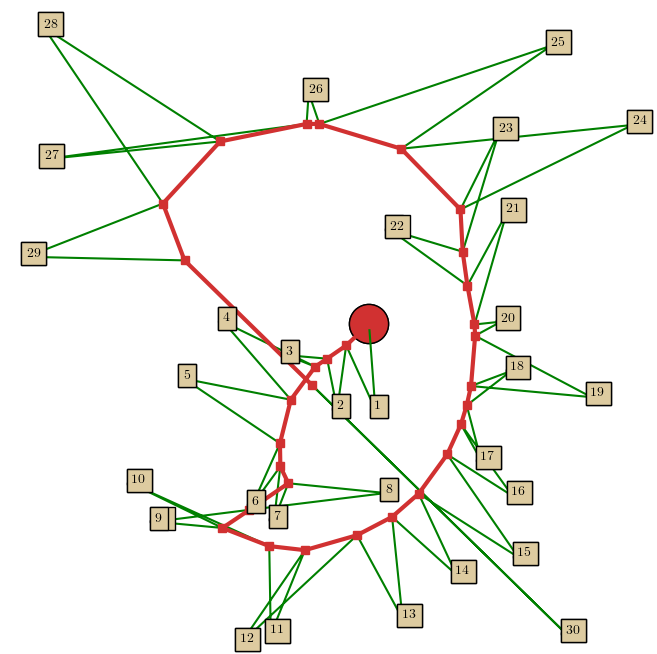
\includegraphics[width=8cm]{../webs/docs/prelim_example_phi5.png}
  \caption{An Example of a classic Horsefly tour with $\varphi=5$. The red dot
    indicates the initial position of the horse and fly, given as part of 
    the input. The ordering of sites shown has been computed with a greedy 
    algorithm which will be described later}
  \label{fig:prelim-example}
\end{figure}


The Horsefly problem is a generalization of the well-known Euclidean Traveling Salesman Problem.
In the most basic version of the Horsefly problem (which we call \textbf{``Classic Horsefly''}), we are given a set of sites, the
initial position of a truck(horse) with a drone(fly) mounted on top, and the speed of the
drone-speed $\varphi$. \footnote{ The speed of the truck is always assumed to be 1 in any of the problem 
  variations we will be considering in this report.} \footnote{ $\varphi$ is also called the ``speed ratio''.}. 

The goal is to compute a tour for both the truck and the drone to deliver package to sites
as quickly as possible. For delivery, a drone must pick up a package from the
truck, fly to the site and come back to the truck to pick up the next package for
delivery to another site. \footnote{ The drone is assumed to be able to carry at most one package at a time }
Both the truck and drone must coordinate their motions to minimize the time it takes for
all the sites to get their packages. Figure \ref{fig:prelim-example} gives an example of such a tour
computed using a greedy heuristic for $\varphi=5$.


This suite of programs implement several experimental heuristics, to solve the above NP-hard
problem and some of its variations approximately. In this short chapter, we give a description 
of the problem variations that we will be tackling. Each of the problems, has a corresponding chapter 
in Part 2, where these heuristics are described and implemented. We also give comparative analyses of 
their experimental performance on various problem instances. 

\vspace{0.5cm}

\begin{description}
\item[Classic Horsefly] This problem has already described in the introduction.

\item[Segment Horsefly] In this variation, the path of the truck is restricted to that of a segment, 
  which we can consider without loss of generality to be $[0,1]$. All sites, without loss of generality 
  lie in the upper-half plane $\RR^2_{+}$. 

\item[Fixed Route Horsefly] This is the obvious generalization of Segment Horsefly, where the path
  which the truck is restricted to travel is a piece-wise linear polygonal path. 
  \footnote{More generally, the truck will be restricted to travelling on a road network, which would 
    typically be modelled as a graph embedded in the plane.} Both the initial 
  position of the truck and the drone are given. The sites to be serviced are allowed to lie anywhere in $\RR^2$. 
  Two further variations are possible in this setting, one in which the truck is allowed reversals
  and the other in which it is not. 

\item[One Horse, Two Flies] The truck is now equipped with two drones. Otherwise the setting, is exactly 
  the same as in classic horsefly. Each drone can carry only one package at a time. The drones must fly back
  and forth between the truck and the sites to deliver the packages. We allow the possibility that 
  both the drones can land at the same time and place on the truck to pick up their next package. \footnote{In reality, 
    one of the drones will have to wait for a small amount of time while the other is retrieving its package. 
    In a more realisting model, we would need to take into account this ``waiting time'' too.}

\item[Reverse Horsefly] In this model, each site (not the truck!) is equipped with a drone, which fly 
  \textit{towards} the truck to pick up their packages. We need to coordinate the motion of the truck 
  and drone so that the time it takes for the last drone to pick up its package (the ``makespan'') is 
  minimized. 

\item[Bounded Distance Horsefly] In most real-world scenarios, the drone will not be able to (or allowed to) go more than
  a certain distance $R$ from the truck. Thus with the same settings as the classic horsefly, but with the added 
  constraint of the drone and the truck never being more than a distance $R$ from the truck, how would one 
  compute the truck and drone paths to minimize the makespan of the deliveries? 

\item[Watchman Horsefly] In place of the TSP, we generalize the Watchman route problem here. 
  \footnote{ although abstractly, the Watchman route problem can be viewed as a kind of TSP}
  We are given as input a simple polygon and the initial position of a truck and a drone. The drone has 
  a camera mounted on top which is assumed to have $360^{\circ}$ vision. Both the truck and drone can move, 
  but the drone can move at most euclidean distance \footnote{The version where instead geodesic distance is 
    considered is also interesting} $R$ from the truck. 

  We want every point in the polygon to be seen by the drone at least once. The goal is to minimize the time it 
  takes for the drone to be able to see every point in the simple polygon. In other words, we want to minimize
  the time it takes for the drone (moving in coordinattion with the truck) to patrol the entire polygon. 
  
\end{description}

\chapter{Installation and Use}

To run these programs you will need to install Docker, an open-source containerization program that is easily installable on 
  Windows 10\footnote{You might need to turn on virtualization explicitly in your BIOS, after installing Docker 
  as I needed to while setting Docker up on Windows. Here is a snapshot of an image when turning on Intel's 
  virtualization technology through the BIOS: 
\url{https://images.techhive.com/images/article/2015/09/virtualbox_vt-x_amd-v_error04_phoenix-100612961-large.idge.jpg}}, MacOS, and almost any 
  GNU/Linux distribution. For a quick introduction to containerization, watch the first two minutes of 
  \url{https://youtu.be/_dfLOzuIg2o}

The nice thing about Docker is that it makes it easy to run softwares on different OS'es portably and neatly side-steps the 
dependency hell problem (\url{https://en.wikipedia.org/wiki/Dependency_hell}.) The headache of installing different library 
dependencies correctly on different machines running different OS'es, is replaced \textbf{only} by learning how to 
install Docker and to set up an X-windows connection between the host OS and an instantiated container running GNU/Linux. 

\begin{alphalist}
\item \crunchy{Get Docker} For installation instrutions watch
  \begin{description}
    \item[GNU/Linux]  \url{https://youtu.be/KCckWweNSrM}
    \item[Windows]    \url{https://youtu.be/ymlWt1MqURY}
    %\item[MacOS]      \url{https://youtu.be/MU8HUVlJTEY}
  \end{description}
  To test your installation, run the \verb|hello-world| container. Note that you might 
  need administrator privileges to run docker. On Windows, you can open the Powershell 
  as an administrator. On GNU/Linux you should use \verb|sudo|
\item \crunchy{Download customized Ubuntu image} \verb| docker pull gtelang/ubuntu_customized| \footnote{The customized Ubuntu image is approximately
  7 GB which contains all the libraries (e.g. CGAL, VTK, numpy, and matplotlib) that I typically use to run 
  my research codes portably.On my home internet connection downloading this Ubuntu-image typically takes about 5-10 minutes. }
\item \crunchy{Clone repository} \verb|git clone gtelang/horseflies_literate.git|
\item \crunchy{Mount and Launch} 
\begin{description}
\item[If you are running GNU/Linux] 
\begin{itemize}
   \item Open up your favorite terminal emulator, such as xterm, rxvt or konsole
   \item Copy to clipboard the output of \texttt{xauth list}
   \item \verb|cd horseflies_literate|
   \item \texttt{docker run -it -\phantom{}-name horsefly\_container -\phantom{}-net=host \textbackslash \newline 
                -e DISPLAY -v /tmp/.X11-unix \textbackslash                                              \newline 
                -v  \`{}pwd\`{}:/horseflies\_mnt gtelang/ubuntu\_customized}
   \item \verb|cd horseflies_mnt| 
   \item \verb|xauth add | \textit{<paste-from-clipboard>}
\end{itemize}

The purpose of using  ``\verb|xauth|'' and ``\verb|-e DISPLAY -v /tmp/.X11-unix|'' is to establish an X-windows connection between your operating 
system and the Ubuntu container that allows you to run GUI apps e.g. the FireFox web-browser. 
\footnote{I found the instructions for running GUI apps on containers in \url{https://www.youtube.com/watch?v=RDg6TRwiPtg}}

\item[If you are running Windows]
  \begin{itemize}
    \item Follow every instruction in \url{https://dev.to/darksmile92/run-gui-app-in-linux-Docker-container-on-windows-host-4kde}.
    \footnote{This step is necessary displaying the Matplotlib canvas as we do in the horseflies project for interactive testing of algorithms.}
      Make sure you can run a gui program like the Firefox web-browser as indicated by the article before going to the next step. 

    \item To mount the horseflies folder, you need to \textit{share} the appropriate drive (e.g. \verb|C:\| or \verb|D:\|) that the \verb|horseflies| folder is in with Docker.
      Follow instructions here: \url{https://rominirani.com/docker-on-windows-mounting-host-directories-d96f3f056a2c}
      for sharing directories. \footnote{you might need administrator privileges to perform this step, as pointed out by the article.}

    \item Open up a Windows Powershell (possibly as administrator)
      \begin{itemize}
           \item \verb|set-variable -name DISPLAY -value <your-ip-address>:0.0| \footnote{You can find your ip-address by the output of the \texttt{ipconfig} command in the Powershell}
           \item \verb|docker run -ti --rm -e DISPLAY=$DISPLAY -v <location-of-horseflies-folder>:/horseflies_mnt  gtelang/ubuntu_customized|
      \end{itemize}
  \end{itemize}

\end{description}

\item \crunchy{Run experiments} If you want to run all the experiments as described in 
  the paper again to reproduce the reported results on your machine, then run \footnote{ Allowing, of course,
  for differences between your machine's CPU and mine when it comes to reporting absolute running time}, \\
  \verb|python main.py --run-all-experiments|. 

  If you want to run a specific experiment, then run \\ \verb|python main.py --run-experiment <experiment-name>|. 

  See Index for a list of all the experiments. 

\item \crunchy{Test algorithms interactively}  If you want to test the algorithms in interactive mode 
  (where you get to select the problem-type, mouse-in the sites on a canvas, set the initial position of 
  the truck and drone and set $\varphi$), run \verb|python main.py --<problem-name>|. The
  list of problems are the same as that given in the previous chapter. The problem name consists
  of all lower-case letters with spaces replaced by hyphens. 

  Thus for instance ``Watchman Horsefly'' becomes \verb|watchman-horsefly| and ``One Horse Two Flies''
  becomes \verb|one-horse-two-flies|. 

  To interactively experiment with different algorithms for, say, the Watchman Horsefly problem , 
  type at the terminal \verb|python main.py --watchman-horsefly|
\end{alphalist}

\vspace{1cm}

If you want to delete the Ubuntu image and any associated containers run the command \footnote{the ubuntu image is 7GB afterall!}
\begin{verbatim}
 docker rm -f horsefly_container; docker rmi -f ubuntu_customized
\end{verbatim}

That's it! Happy horseflying!
\part{Programs}
\chapter{Overview of the Code Base}

All of the code has been written in Python 2.7 and tested using the standard CPython
implementation of the language. In some cases, calls will be made to external C\texttt{++} 
libraries (mostly CGAL and VTK) using SWIG (\url{http://www.swig.org/})
for speeding up a slow routine or to use a function that is not available in any existing 
Python package.

\section{Source Tree}
\begin{verbatim}
..
|-- horseflies.pdf -> tex/horseflies.pdf
|-- main.py
|-- scrap.test
|-- src
|   |-- expts
|   |-- lib
|   |   |-- problem_classic_horsefly.py
|   |   |-- utils_algo.py
|   |   `-- utils_graphics.py
|   |-- Makefile
|   `-- tests
|-- tex
|   |-- directory-tree.tex
|   |-- horseflies.pdf
|   |-- horseflies.tex
|   `-- standard_settings.tex
`-- webs
    |-- algo-dumb-classic-horsefly.web
    |-- algo-greedy-nn-classic-horsefly.web
    |-- descriptions-of-problems.web
    |-- horseflies.web
    |-- installation-and-use.web
    |-- overview-of-code-base.web
    |-- problem-classic-horsefly.web
    |-- problem-fixed-route-horsefly.web
    |-- problem-one-horse-two-flies.web
    |-- problem-reverse-horsefly.web
    |-- problem-segment-horsefly.web
    |-- problem-watchman-horsefly.web
    |-- utility-functions.web
    `-- weave-tangle.sh

6 directories, 25 files
\end{verbatim}


There are three principal directories 
\begin{itemize}

 \item[\texttt{webs/}] This contains the source code for the entire project written in 
                       the nuweb format along with documents (mostly images)
                       needed during the compilation of the \LaTeX{} files which will 
                       be extracted from the \texttt{.web} files. 

 \item[\texttt{src/}] This contains the source code for the entire project ``tangled'' 
                      (i.e. extracted) from the \texttt{.web} files. 
 \item[\texttt{tex/}] This contains the monolithic \texttt{horseflies.tex} extracted 
                      from the \texttt{.web} files and a bunch 
                      of other supporing \LaTeX{} files. It also contains the final 
                      compiled \texttt{horseflies.pdf} (the current document) which 
                      contains the documentation of the project, interwoven with 
                      code-chunks and cross-references between them along with the 
                      experimental results.  
\end{itemize}  

The files in \texttt{src} and \texttt{tex} should not be touched. Any editing required should 
be done directly to the \texttt{.web} files which should then be weaved and tangled 
using \texttt{weave-tangle.sh}. 

\section{The Main Files} 

\newchunk 
\begin{alphalist}

\item \crunchy{\texttt{main.py}} The file \verb|main.py| in the top-level folder is the 
\textit{entry-point} for running code. Its only job is to parse the 
command-line arguments and pass relevant information to the handler 
functions for each problem and experiment. 

\TODO{Add an item containing the interface files. Do this for the Haskell files that 
you will ultimately add in later.}

\item \crunchy{Algorithmic Code} All such files are in the directory \texttt{src/lib/}.
  Each of the files with prefix ``\verb|problem_*|'' contain implmentations of 
  algorithms for one specific problem. For instance \verb|problem_watchman_horsefly.py| 
  contains algorithms for approximately solving the Watchman Horsefly problem. 
 
  Since Horsefly-type problems are typically NP-hard, an important factor in 
  the subsequent experimental analysis will require, comparing an algorithm's  
  output against good lower bounds. Each such file, will also have routines
  for efficiently computing or approximating various lower-bounds for the 
  corresponding problem's \textit{OPT}. 

\item \crunchy{Experiments} All such files are in the directory \texttt{src/expt/}
 Each of the files with prefix ``\verb|expt_*|'' 
 contain code for testing hypotheses regarding a problem, generating 
 counter-examples or comparing the experimental performance of the 
 algorithm implementations for each of the problems. Thus 
 \verb|expt_watchman_horsefly.py| contains 
 code for performing experiments related to the 
 Watchman Horsefly problem. 
\end{alphalist}


If you need to edit the source-code for algorithms or experiment 
you should do so to the \texttt{.web} files in the web directory. Every problem
has a dedicated \textit{folder} containing source-code for algorithms and experiments 
pertaining to that problem. Every algorithm and experiment has a dedicated \verb|.web|
file in these problem directories. Such files are all ``tied'' together using the 
file with prefix \verb|problem-<problem-name>| in that same directory (i.e.
the file acts as a kind of handler for each problem, that includes the algorithms
and experiment \verb|web| files with the \verb|@i| macro.) 


\newchunk Let's define the \verb|main.py| file now. 

Each problem or experiment has a handler routine 
that effectively acts as a kind of ``main'' function for that module that 
does house-keeping duties by parsing the command-line arguments passed by main, 
setting up the canvas by calling the appropriate graphics routines and calling 
the algorithms on the input specified through the canvas. 

%{python-mode}%
\begin{flushleft} \small
\begin{minipage}{\linewidth}\label{scrap1}\raggedright\small
\NWtarget{nuweb12}{} \verb@"../main.py"@\nobreak\ {\footnotesize {12}}$\equiv$
\vspace{-1ex}
\begin{list}{}{} \item
\mbox{}\verb@@\\
\mbox{}\verb@@\hbox{$\langle\,${\itshape Turn off Matplotlibs irritating DEBUG messages}\nobreak\ {\footnotesize \NWlink{nuweb13a}{13a}}$\,\rangle$}\verb@@\\
\mbox{}\verb@@\hbox{$\langle\,${\itshape Import problem module files}\nobreak\ {\footnotesize \NWlink{nuweb13b}{13b}}$\,\rangle$}\verb@@\\
\mbox{}\verb@@\\
\mbox{}\verb@if __name__=="__main__":@\\
\mbox{}\verb@     # Select algorithm or experiment @\\
\mbox{}\verb@     if (len(sys.argv)==1):@\\
\mbox{}\verb@          print "Specify the problem or experiment you want to run"@\\
\mbox{}\verb@          sys.exit()@\\
\mbox{}\verb@@\\
\mbox{}\verb@     elif sys.argv[1] == "--problem-classic-horsefly":@\\
\mbox{}\verb@          chf.run_handler()@\\
\mbox{}\verb@@\\
\mbox{}\verb@     elif sys.argv[1] == "--problem-one-horse-multiple-flies":@\\
\mbox{}\verb@          ohmf.run_handler()@\\
\mbox{}\verb@@\\
\mbox{}\verb@     else:@\\
\mbox{}\verb@          print "Option not recognized"@\\
\mbox{}\verb@          sys.exit()@\\
\mbox{}\verb@@{\NWsep}
\end{list}
\vspace{-1.5ex}
\footnotesize
\begin{list}{}{\setlength{\itemsep}{-\parsep}\setlength{\itemindent}{-\leftmargin}}

\item{}
\end{list}
\end{minipage}\vspace{4ex}
\end{flushleft}
%{/python-mode}%

\newchunk On my customized Ubuntu container, Matplotlib produces tons of DEBUG log messages because  
it recently switched to the \verb|logging| library for...well...logging. 
The lines in this chunk were suggested by the link 
\url{http://matplotlib.1069221.n5.nabble.com/How-to-turn-off-matplotlib-DEBUG-msgs-td48822.html} 
for quietening down Matplotlib.  


%{python-mode}%
\begin{flushleft} \small
\begin{minipage}{\linewidth}\label{scrap2}\raggedright\small
\NWtarget{nuweb13a}{} $\langle\,${\itshape Turn off Matplotlibs irritating DEBUG messages}\nobreak\ {\footnotesize {13a}}$\,\rangle\equiv$
\vspace{-1ex}
\begin{list}{}{} \item
\mbox{}\verb@import logging@\\
\mbox{}\verb@mpl_logger = logging.getLogger('matplotlib')@\\
\mbox{}\verb@mpl_logger.setLevel(logging.WARNING)@\\
\mbox{}\verb@@{\NWsep}
\end{list}
\vspace{-1.5ex}
\footnotesize
\begin{list}{}{\setlength{\itemsep}{-\parsep}\setlength{\itemindent}{-\leftmargin}}
\item \NWtxtMacroRefIn\ \NWlink{nuweb12}{12}.

\item{}
\end{list}
\end{minipage}\vspace{4ex}
\end{flushleft}
%{/python-mode}%

%{python-mode}%
\begin{flushleft} \small
\begin{minipage}{\linewidth}\label{scrap3}\raggedright\small
\NWtarget{nuweb13b}{} $\langle\,${\itshape Import problem module files}\nobreak\ {\footnotesize {13b}}$\,\rangle\equiv$
\vspace{-1ex}
\begin{list}{}{} \item
\mbox{}\verb@   @\\
\mbox{}\verb@import sys@\\
\mbox{}\verb@sys.path.append('src/lib')@\\
\mbox{}\verb@import problem_classic_horsefly as chf@\\
\mbox{}\verb@import problem_one_horse_multiple_flies as ohmf@\\
\mbox{}\verb@@{\NWsep}
\end{list}
\vspace{-1.5ex}
\footnotesize
\begin{list}{}{\setlength{\itemsep}{-\parsep}\setlength{\itemindent}{-\leftmargin}}
\item \NWtxtMacroRefIn\ \NWlink{nuweb12}{12}.

\item{}
\end{list}
\end{minipage}\vspace{4ex}
\end{flushleft}
%{/python-mode}%
\section{Support Files}

\begin{alphalist}
\item \crunchy{Utility Files}  All such utility files are in the directory \texttt{src/lib/}. 
 These files contain common utility functions  for manipulating data-structures, plotting 
 and graphics routines common to all horsefly-type problems. All such files have the prefix 
 \verb|utils_*|. These Python files are generated from the single \verb|.web| file \verb|utils.web| 
 in the \verb|web| subdirectory.

\item \crunchy{Tests} All such files are in the directory \texttt{src/test/}
 To automate testing of code during implementations, tests for various 
 routines across the entire code-base have been written in files with prefix
 \verb|test_*|.  
 
 Every problem, utility, and experimental files in \verb|src/lib| and \verb|src/expts| 
 has a corresponding test-file in this folder. 
\end{alphalist}\chapter{Some (Boring) Utility Functions}
\label{chap:utility-functions}

We will be needing some utility functions, for drawing and manipulating data-structures 
which will be implemented in files separate from \verb|problem_classic_horsefly.py|.  All such
files will be prefixed with the work \verb|utils_|. Many of the important common utility 
functions are defined here; others will be defined on the fly throughout the rest of the report. 
This chapter just collects the most important of the functions for the sake of clarity of exposition
in the later chapters. 

\section{Graphical Utilities}

Here we will  develop routines to interactively insert points onto a Matplotlib canvas and clear the canvas. 
Almost all variants of the horsefly problem will involve mousing in sites and the initial position of the horse 
and fly. These points will typically be represented by small circular patches. The type of the point
will be indicated by its color and size e.g. intial position of truck and drone 
will typically be represented by a large red dot while and the sites by smaller blue dots. 

Matplotlib has extensive support for inserting such circular patches onto its canvas with 
mouse-clicks. Each such graphical canvas corresponds (roughly) to Matplotlib figure
object instance. Each figure consists of several Axes objects which contains
most of the figure elements i.e. the Axes objects correspond to the ``drawing area''
of the canvas. 

\newchunk First we set up the axes limits, dimensions and other configuration quantities
which will correspond to the ``without loss of generality'' assumptions made in the 
statements of the horsefly problems. We also need to set up the axes limits,
dimensions, and other fluff. The following fragment defines a function which 
``normalizes'' a drawing area by setting up the x and y limits and making the 
aspect ratio of the axes object the same i.e. 1.0. Since Matplotlib is principally
a plotting software, this is not the default behavior, since scales on the x and y 
axes are adjusted according to the data to be plotted. 

%{python-mode}%
\begin{flushleft} \small\label{scrap4}\raggedright\small
\NWtarget{nuweb14}{} \verb@"../src/lib/utils_graphics.py"@\nobreak\ {\footnotesize {14}}$\equiv$
\vspace{-1ex}
\begin{list}{}{} \item
\mbox{}\verb@@\\
\mbox{}\verb@@\\
\mbox{}\verb@from matplotlib import rc@\\
\mbox{}\verb@from colorama import Fore@\\
\mbox{}\verb@from colorama import Style@\\
\mbox{}\verb@from scipy.optimize import minimize@\\
\mbox{}\verb@from sklearn.cluster import KMeans@\\
\mbox{}\verb@import argparse@\\
\mbox{}\verb@import itertools@\\
\mbox{}\verb@import math@\\
\mbox{}\verb@import matplotlib as mpl@\\
\mbox{}\verb@import matplotlib.pyplot as plt@\\
\mbox{}\verb@import numpy as np@\\
\mbox{}\verb@import os@\\
\mbox{}\verb@import pprint as pp@\\
\mbox{}\verb@import randomcolor @\\
\mbox{}\verb@import sys@\\
\mbox{}\verb@import time@\\
\mbox{}\verb@@\\
\mbox{}\verb@xlim, ylim = [0,1], [0,1]@\\
\mbox{}\verb@@\\
\mbox{}\verb@def applyAxCorrection(ax):@\\
\mbox{}\verb@      ax.set_xlim([xlim[0], xlim[1]])@\\
\mbox{}\verb@      ax.set_ylim([ylim[0], ylim[1]])@\\
\mbox{}\verb@      ax.set_aspect(1.0)@\\
\mbox{}\verb@@{\NWsep}
\end{list}
\vspace{-1.5ex}
\footnotesize
\begin{list}{}{\setlength{\itemsep}{-\parsep}\setlength{\itemindent}{-\leftmargin}}
\item \NWtxtFileDefBy\ \NWlink{nuweb14}{14}\NWlink{nuweb15a}{, 15a}\NWlink{nuweb15b}{b}\NWlink{nuweb15c}{c}\NWlink{nuweb16d}{, 16d}.

\item{}
\end{list}
\vspace{4ex}
\end{flushleft}
%{/python-mode}%
\vspace{-0.8cm}
\newchunk Next, given an axes object (i.e. a drawing area on a figure object) we need a function
to delete and remove all the graphical objects drawn on it. 

%{python-mode}%
\begin{flushleft} \small\label{scrap5}\raggedright\small
\NWtarget{nuweb15a}{} \verb@"../src/lib/utils_graphics.py"@\nobreak\ {\footnotesize {15a}}$\equiv$
\vspace{-1ex}
\begin{list}{}{} \item
\mbox{}\verb@@\\
\mbox{}\verb@def clearPatches(ax):@\\
\mbox{}\verb@    # Get indices cooresponding to the polygon patches@\\
\mbox{}\verb@    for index , patch in zip(range(len(ax.patches)), ax.patches):@\\
\mbox{}\verb@        if isinstance(patch, mpl.patches.Polygon) == True:@\\
\mbox{}\verb@            patch.remove()@\\
\mbox{}\verb@    ax.lines[:]=[]@\\
\mbox{}\verb@    applyAxCorrection(ax)@\\
\mbox{}\verb@@{\NWsep}
\end{list}
\vspace{-1.5ex}
\footnotesize
\begin{list}{}{\setlength{\itemsep}{-\parsep}\setlength{\itemindent}{-\leftmargin}}
\item \NWtxtFileDefBy\ \NWlink{nuweb14}{14}\NWlink{nuweb15a}{, 15a}\NWlink{nuweb15b}{b}\NWlink{nuweb15c}{c}\NWlink{nuweb16d}{, 16d}.

\item{}
\end{list}
\vspace{4ex}
\end{flushleft}
%{/python-mode}%

\vspace{-0.8cm}
\newchunk Now remove the patches which were rendered for each cluster
    Unfortunately, this step has to be done manually, the canvas patch
    of a cluster and the corresponding object in memory are not reactively
    connected.I presume, this behavioue can be achieved by sub-classing.

%{python-mode}%
\begin{flushleft} \small\label{scrap6}\raggedright\small
\NWtarget{nuweb15b}{} \verb@"../src/lib/utils_graphics.py"@\nobreak\ {\footnotesize {15b}}$\equiv$
\vspace{-1ex}
\begin{list}{}{} \item
\mbox{}\verb@@\\
\mbox{}\verb@def clearAxPolygonPatches(ax):@\\
\mbox{}\verb@@\\
\mbox{}\verb@    # Get indices cooresponding to the polygon patches@\\
\mbox{}\verb@    for index , patch in zip(range(len(ax.patches)), ax.patches):@\\
\mbox{}\verb@        if isinstance(patch, mpl.patches.Polygon) == True:@\\
\mbox{}\verb@            patch.remove()@\\
\mbox{}\verb@    ax.lines[:]=[]@\\
\mbox{}\verb@    applyAxCorrection(ax)@\\
\mbox{}\verb@@{\NWsep}
\end{list}
\vspace{-1.5ex}
\footnotesize
\begin{list}{}{\setlength{\itemsep}{-\parsep}\setlength{\itemindent}{-\leftmargin}}
\item \NWtxtFileDefBy\ \NWlink{nuweb14}{14}\NWlink{nuweb15a}{, 15a}\NWlink{nuweb15b}{b}\NWlink{nuweb15c}{c}\NWlink{nuweb16d}{, 16d}.

\item{}
\end{list}
\vspace{4ex}
\end{flushleft}
%{/python-mode}%
\newchunk Now for one of the most important routines for drawing on the canvas! 
To insert the sites, we double-click the left mouse button and to insert the 
initial position of the horse and fly we double-click the right mouse-button. 

The following chunk defines a function that creates a closure for a mouseclick 
even on the matplotlib canvas. 

Note that the left mouse-button corresponds to button 1 and right mouse button
to button 3 in the code-fragment below. 

\TODO{Remove the previous red patches, 
which contain the old position
of the horse and fly. Doing this is 
slightly painful, hence keeping it
for later.}

%{python-mode}%
\begin{flushleft} \small\label{scrap7}\raggedright\small
\NWtarget{nuweb15c}{} \verb@"../src/lib/utils_graphics.py"@\nobreak\ {\footnotesize {15c}}$\equiv$
\vspace{-1ex}
\begin{list}{}{} \item
\mbox{}\verb@def wrapperEnterRunPoints(fig, ax, run):@\\
\mbox{}\verb@    def _enterPoints(event):@\\
\mbox{}\verb@        if event.name      == 'button_press_event'          and \@\\
\mbox{}\verb@           (event.button   == 1 or event.button == 3)       and \@\\
\mbox{}\verb@            event.dblclick == True and event.xdata  != None and event.ydata  != None:@\\
\mbox{}\verb@@\\
\mbox{}\verb@             if event.button == 1:  @\\
\mbox{}\verb@                 @\hbox{$\langle\,${\itshape Insert blue circle representing a site}\nobreak\ {\footnotesize \NWlink{nuweb16a}{16a}}$\,\rangle$}\verb@@\\
\mbox{}\verb@@\\
\mbox{}\verb@             elif event.button == 3:  @\\
\mbox{}\verb@                 @\hbox{$\langle\,${\itshape Insert big red circle representing initial position of horse and fly}\nobreak\ {\footnotesize \NWlink{nuweb16b}{16b}}$\,\rangle$}\verb@@\\
\mbox{}\verb@@\\
\mbox{}\verb@             @\hbox{$\langle\,${\itshape Clear polygon patches and set up last minute \verb|ax| tweaks}\nobreak\ {\footnotesize \NWlink{nuweb16c}{16c}}$\,\rangle$}\verb@@\\
\mbox{}\verb@@\\
\mbox{}\verb@    return _enterPoints@\\
\mbox{}\verb@@{\NWsep}
\end{list}
\vspace{-1.5ex}
\footnotesize
\begin{list}{}{\setlength{\itemsep}{-\parsep}\setlength{\itemindent}{-\leftmargin}}
\item \NWtxtFileDefBy\ \NWlink{nuweb14}{14}\NWlink{nuweb15a}{, 15a}\NWlink{nuweb15b}{b}\NWlink{nuweb15c}{c}\NWlink{nuweb16d}{, 16d}.

\item{}
\end{list}
\vspace{4ex}
\end{flushleft}
%{/python-mode}%

\vspace{-0.8cm} \newchunk
%{python-mode}%
\begin{flushleft} \small
\begin{minipage}{\linewidth}\label{scrap8}\raggedright\small
\NWtarget{nuweb16a}{} $\langle\,${\itshape Insert blue circle representing a site}\nobreak\ {\footnotesize {16a}}$\,\rangle\equiv$
\vspace{-1ex}
\begin{list}{}{} \item
\mbox{}\verb@  @\\
\mbox{}\verb@newPoint = (event.xdata, event.ydata)@\\
\mbox{}\verb@run.sites.append( newPoint  )@\\
\mbox{}\verb@patchSize  = (xlim[1]-xlim[0])/140.0@\\
\mbox{}\verb@   @\\
\mbox{}\verb@ax.add_patch( mpl.patches.Circle( newPoint, radius = patchSize,@\\
\mbox{}\verb@                                  facecolor='blue', edgecolor='black'  ))@\\
\mbox{}\verb@ax.set_title('Points Inserted: ' + str(len(run.sites)), \@\\
\mbox{}\verb@             fontdict={'fontsize':40})@\\
\mbox{}\verb@@{\NWsep}
\end{list}
\vspace{-1.5ex}
\footnotesize
\begin{list}{}{\setlength{\itemsep}{-\parsep}\setlength{\itemindent}{-\leftmargin}}
\item \NWtxtMacroRefIn\ \NWlink{nuweb15c}{15c}.

\item{}
\end{list}
\end{minipage}\vspace{4ex}
\end{flushleft}
%{/python-mode}%

\vspace{-0.8cm} \newchunk
%{python-mode}%
\begin{flushleft} \small
\begin{minipage}{\linewidth}\label{scrap9}\raggedright\small
\NWtarget{nuweb16b}{} $\langle\,${\itshape Insert big red circle representing initial position of horse and fly}\nobreak\ {\footnotesize {16b}}$\,\rangle\equiv$
\vspace{-1ex}
\begin{list}{}{} \item
\mbox{}\verb@ @\\
\mbox{}\verb@inithorseposn     = (event.xdata, event.ydata)@\\
\mbox{}\verb@run.inithorseposn = inithorseposn  @\\
\mbox{}\verb@patchSize         = (xlim[1]-xlim[0])/100.0@\\
\mbox{}\verb@@\\
\mbox{}\verb@ax.add_patch( mpl.patches.Circle( inithorseposn,radius = patchSize,@\\
\mbox{}\verb@                                  facecolor= '#D13131', edgecolor='black' ))@\\
\mbox{}\verb@@{\NWsep}
\end{list}
\vspace{-1.5ex}
\footnotesize
\begin{list}{}{\setlength{\itemsep}{-\parsep}\setlength{\itemindent}{-\leftmargin}}
\item \NWtxtMacroRefIn\ \NWlink{nuweb15c}{15c}.

\item{}
\end{list}
\end{minipage}\vspace{4ex}
\end{flushleft}
%{/python-mode}%



\vspace{-0.8cm} \newchunk   
 It is inefficient to clear the polygon patches \textit{inside} the
 \verb|enterRunpoints| event loop as done here. However, this has just been done for 
 simplicity: the intended behaviour at any rate, is to clear all the polygon patches \
 from the axes object, once the user starts entering in more points to the cloud
 for which the clustering was just computed and rendered. The moment the user starts 
 entering new points, the previous polygon patches are garbage collected. 

%{python-mode}%
\begin{flushleft} \small
\begin{minipage}{\linewidth}\label{scrap10}\raggedright\small
\NWtarget{nuweb16c}{} $\langle\,${\itshape Clear polygon patches and set up last minute \verb|ax| tweaks}\nobreak\ {\footnotesize {16c}}$\,\rangle\equiv$
\vspace{-1ex}
\begin{list}{}{} \item
\mbox{}\verb@   @\\
\mbox{}\verb@clearAxPolygonPatches(ax)@\\
\mbox{}\verb@applyAxCorrection(ax)@\\
\mbox{}\verb@fig.canvas.draw()@\\
\mbox{}\verb@@{\NWsep}
\end{list}
\vspace{-1.5ex}
\footnotesize
\begin{list}{}{\setlength{\itemsep}{-\parsep}\setlength{\itemindent}{-\leftmargin}}
\item \NWtxtMacroRefIn\ \NWlink{nuweb15c}{15c}.

\item{}
\end{list}
\end{minipage}\vspace{4ex}
\end{flushleft}
%{/python-mode}%



\newchunk  We also need a function to generate a specified number of visually distinct colors, especially
when dealing with  multiple flies. 

%{python-mode}%
\begin{flushleft} \small\label{scrap11}\raggedright\small
\NWtarget{nuweb16d}{} \verb@"../src/lib/utils_graphics.py"@\nobreak\ {\footnotesize {16d}}$\equiv$
\vspace{-1ex}
\begin{list}{}{} \item
\mbox{}\verb@@\\
\mbox{}\verb@# Borrowed from https://stackoverflow.com/a/9701141@\\
\mbox{}\verb@import numpy as np@\\
\mbox{}\verb@import colorsys@\\
\mbox{}\verb@@\\
\mbox{}\verb@def get_colors(num_colors, lightness=0.2):@\\
\mbox{}\verb@    colors=[]@\\
\mbox{}\verb@    for i in np.arange(60., 360., 300. / num_colors):@\\
\mbox{}\verb@        hue        = i/360.0@\\
\mbox{}\verb@        saturation = 0.95@\\
\mbox{}\verb@        colors.append(colorsys.hls_to_rgb(hue, lightness, saturation))@\\
\mbox{}\verb@    return colors@\\
\mbox{}\verb@@{\NWsep}
\end{list}
\vspace{-1.5ex}
\footnotesize
\begin{list}{}{\setlength{\itemsep}{-\parsep}\setlength{\itemindent}{-\leftmargin}}
\item \NWtxtFileDefBy\ \NWlink{nuweb14}{14}\NWlink{nuweb15a}{, 15a}\NWlink{nuweb15b}{b}\NWlink{nuweb15c}{c}\NWlink{nuweb16d}{, 16d}.

\item{}
\end{list}
\vspace{4ex}
\end{flushleft}
%{/python-mode}%


\section{Algorithmic Utilities}

\newchunk Given a list of  points $[p_0,p_1,p_2,....p_{n-1}]$. 
    the following function returns, $[p_1-p_0, p_2-p_1,...,p_{n-1}-p_{n-2}]$
    i.e. it converts the list of points into a consecutive list of numpy vectors. 
    Points should be lists or tuples of length 2

%{python-mode}%
\begin{flushleft} \small\label{scrap12}\raggedright\small
\NWtarget{nuweb17a}{} \verb@"../src/lib/utils_algo.py"@\nobreak\ {\footnotesize {17a}}$\equiv$
\vspace{-1ex}
\begin{list}{}{} \item
\mbox{}\verb@@\\
\mbox{}\verb@import numpy as np@\\
\mbox{}\verb@import random@\\
\mbox{}\verb@from colorama import Fore@\\
\mbox{}\verb@from colorama import Style@\\
\mbox{}\verb@@\\
\mbox{}\verb@@\\
\mbox{}\verb@def vector_chain_from_point_list(pts):@\\
\mbox{}\verb@    vec_chain = []@\\
\mbox{}\verb@    for pair in zip(pts, pts[1:]):@\\
\mbox{}\verb@        tail= np.array (pair[0])@\\
\mbox{}\verb@        head= np.array (pair[1])@\\
\mbox{}\verb@        vec_chain.append(head-tail)@\\
\mbox{}\verb@@\\
\mbox{}\verb@    return vec_chain@\\
\mbox{}\verb@@{\NWsep}
\end{list}
\vspace{-1.5ex}
\footnotesize
\begin{list}{}{\setlength{\itemsep}{-\parsep}\setlength{\itemindent}{-\leftmargin}}
\item \NWtxtFileDefBy\ \NWlink{nuweb17a}{17a}\NWlink{nuweb17b}{b}\NWlink{nuweb18a}{, 18a}\NWlink{nuweb18b}{b}\NWlink{nuweb18c}{c}\NWlink{nuweb18d}{d}\NWlink{nuweb18e}{e}\NWlink{nuweb18f}{f}\NWlink{nuweb19c}{, 19c}.

\item{}
\end{list}
\vspace{4ex}
\end{flushleft}
%{/python-mode}%

\newchunk Given a polygonal chain in the form of successive points  $[p_0,p_1,p_2,....p_{n-1}]$, 
an important computation is to calculate its length. Points should be lists or tuples of length 2
If no points or just one point is given in the list of points, then 0 is returned.

Typically used for computing the length of the horse's and fly's tours. 

%{python-mode}%
\begin{flushleft} \small\label{scrap13}\raggedright\small
\NWtarget{nuweb17b}{} \verb@"../src/lib/utils_algo.py"@\nobreak\ {\footnotesize {17b}}$\equiv$
\vspace{-1ex}
\begin{list}{}{} \item
\mbox{}\verb@@\\
\mbox{}\verb@def length_polygonal_chain(pts):@\\
\mbox{}\verb@    vec_chain = vector_chain_from_point_list(pts)@\\
\mbox{}\verb@@\\
\mbox{}\verb@    acc = 0@\\
\mbox{}\verb@    for vec in vec_chain:@\\
\mbox{}\verb@        acc = acc + np.linalg.norm(vec)@\\
\mbox{}\verb@    return acc@\\
\mbox{}\verb@@{\NWsep}
\end{list}
\vspace{-1.5ex}
\footnotesize
\begin{list}{}{\setlength{\itemsep}{-\parsep}\setlength{\itemindent}{-\leftmargin}}
\item \NWtxtFileDefBy\ \NWlink{nuweb17a}{17a}\NWlink{nuweb17b}{b}\NWlink{nuweb18a}{, 18a}\NWlink{nuweb18b}{b}\NWlink{nuweb18c}{c}\NWlink{nuweb18d}{d}\NWlink{nuweb18e}{e}\NWlink{nuweb18f}{f}\NWlink{nuweb19c}{, 19c}.

\item{}
\end{list}
\vspace{4ex}
\end{flushleft}
%{/python-mode}%
\newchunk The following routine is useful on long lists returned from external solvers. 
Often point-data is given to and returned from these external routines in flattened
form. The following routines are needed to convert such a ``flattened'' list into 
a list of points and vice versa. 

Convert a vector of even length into a vector of points. i.e. 
$[x_0,x_1,x_2,...x_{2n}] \rarr [[x_0,x_1],[x_2,x_3],,..[x_{2n-1},x_{2n}]]$


%{python-mode}%
\begin{flushleft} \small
\begin{minipage}{\linewidth}\label{scrap14}\raggedright\small
\NWtarget{nuweb18a}{} \verb@"../src/lib/utils_algo.py"@\nobreak\ {\footnotesize {18a}}$\equiv$
\vspace{-1ex}
\begin{list}{}{} \item
\mbox{}\verb@def pointify_vector (x):@\\
\mbox{}\verb@    if len(x) % 2 == 0:@\\
\mbox{}\verb@        pts = []@\\
\mbox{}\verb@        for i in range(len(x))[::2]:@\\
\mbox{}\verb@            pts.append( [x[i],x[i+1]] )@\\
\mbox{}\verb@        return pts@\\
\mbox{}\verb@    else :@\\
\mbox{}\verb@        sys.exit('List of items does not have an even length to be able to be pointifyed')@\\
\mbox{}\verb@@{\NWsep}
\end{list}
\vspace{-1.5ex}
\footnotesize
\begin{list}{}{\setlength{\itemsep}{-\parsep}\setlength{\itemindent}{-\leftmargin}}
\item \NWtxtFileDefBy\ \NWlink{nuweb17a}{17a}\NWlink{nuweb17b}{b}\NWlink{nuweb18a}{, 18a}\NWlink{nuweb18b}{b}\NWlink{nuweb18c}{c}\NWlink{nuweb18d}{d}\NWlink{nuweb18e}{e}\NWlink{nuweb18f}{f}\NWlink{nuweb19c}{, 19c}.

\item{}
\end{list}
\end{minipage}\vspace{4ex}
\end{flushleft}
%{/python-mode}%

\vspace{-0.8cm}
The next chunk peforms the opposite process i.e. it flatten's the vector
e.g. $[[0,1],[2,3],[4,5]] \rarr [0,1,2,3,4,5]$


%{python-mode}%
\begin{flushleft} \small
\begin{minipage}{\linewidth}\label{scrap15}\raggedright\small
\NWtarget{nuweb18b}{} \verb@"../src/lib/utils_algo.py"@\nobreak\ {\footnotesize {18b}}$\equiv$
\vspace{-1ex}
\begin{list}{}{} \item
\mbox{}\verb@def flatten_list_of_lists(l):@\\
\mbox{}\verb@       return [item for sublist in l for item in sublist]@\\
\mbox{}\verb@@{\NWsep}
\end{list}
\vspace{-1.5ex}
\footnotesize
\begin{list}{}{\setlength{\itemsep}{-\parsep}\setlength{\itemindent}{-\leftmargin}}
\item \NWtxtFileDefBy\ \NWlink{nuweb17a}{17a}\NWlink{nuweb17b}{b}\NWlink{nuweb18a}{, 18a}\NWlink{nuweb18b}{b}\NWlink{nuweb18c}{c}\NWlink{nuweb18d}{d}\NWlink{nuweb18e}{e}\NWlink{nuweb18f}{f}\NWlink{nuweb19c}{, 19c}.

\item{}
\end{list}
\end{minipage}\vspace{4ex}
\end{flushleft}
%{/python-mode}%

\vspace{-0.8cm}
\newchunk Python's default print function prints each list on a single line. For 
debugging purposes,  it helps to print a list with one item per line. 

%{python-mode}%
\begin{flushleft} \small\label{scrap16}\raggedright\small
\NWtarget{nuweb18c}{} \verb@"../src/lib/utils_algo.py"@\nobreak\ {\footnotesize {18c}}$\equiv$
\vspace{-1ex}
\begin{list}{}{} \item
\mbox{}\verb@def print_list(xs):@\\
\mbox{}\verb@    for x in xs:@\\
\mbox{}\verb@        print x@\\
\mbox{}\verb@@{\NWsep}
\end{list}
\vspace{-1.5ex}
\footnotesize
\begin{list}{}{\setlength{\itemsep}{-\parsep}\setlength{\itemindent}{-\leftmargin}}
\item \NWtxtFileDefBy\ \NWlink{nuweb17a}{17a}\NWlink{nuweb17b}{b}\NWlink{nuweb18a}{, 18a}\NWlink{nuweb18b}{b}\NWlink{nuweb18c}{c}\NWlink{nuweb18d}{d}\NWlink{nuweb18e}{e}\NWlink{nuweb18f}{f}\NWlink{nuweb19c}{, 19c}.

\item{}
\end{list}
\vspace{4ex}
\end{flushleft}
%{/python-mode}%

\vspace{-0.8cm}
\newchunk This chunk just calculates the list of partial sums e.g. $[4,2,3] \rarr [4,6,9]"$
%{python-mode}%
\begin{flushleft} \small\label{scrap17}\raggedright\small
\NWtarget{nuweb18d}{} \verb@"../src/lib/utils_algo.py"@\nobreak\ {\footnotesize {18d}}$\equiv$
\vspace{-1ex}
\begin{list}{}{} \item
\mbox{}\verb@def partial_sums( xs ):@\\
\mbox{}\verb@    psum = 0@\\
\mbox{}\verb@    acc = []@\\
\mbox{}\verb@    for x in xs:@\\
\mbox{}\verb@        psum = psum+x@\\
\mbox{}\verb@        acc.append( psum )@\\
\mbox{}\verb@    return acc@\\
\mbox{}\verb@@{\NWsep}
\end{list}
\vspace{-1.5ex}
\footnotesize
\begin{list}{}{\setlength{\itemsep}{-\parsep}\setlength{\itemindent}{-\leftmargin}}
\item \NWtxtFileDefBy\ \NWlink{nuweb17a}{17a}\NWlink{nuweb17b}{b}\NWlink{nuweb18a}{, 18a}\NWlink{nuweb18b}{b}\NWlink{nuweb18c}{c}\NWlink{nuweb18d}{d}\NWlink{nuweb18e}{e}\NWlink{nuweb18f}{f}\NWlink{nuweb19c}{, 19c}.

\item{}
\end{list}
\vspace{4ex}
\end{flushleft}
%{/python-mode}%

\vspace{-0.8cm}
\newchunk For two given lists of points test if they are 
equal or not. We do this by checking the $L^{\infty}$ norm.
%{python-mode}%
\begin{flushleft} \small
\begin{minipage}{\linewidth}\label{scrap18}\raggedright\small
\NWtarget{nuweb18e}{} \verb@"../src/lib/utils_algo.py"@\nobreak\ {\footnotesize {18e}}$\equiv$
\vspace{-1ex}
\begin{list}{}{} \item
\mbox{}\verb@def are_site_orderings_equal(sites1, sites2):@\\
\mbox{}\verb@@\\
\mbox{}\verb@    for (x1,y1), (x2,y2) in zip(sites1, sites2): @\\
\mbox{}\verb@        if (x1-x2)**2 + (y1-y2)**2 > 1e-8:@\\
\mbox{}\verb@            return False@\\
\mbox{}\verb@    return True@\\
\mbox{}\verb@@{\NWsep}
\end{list}
\vspace{-1.5ex}
\footnotesize
\begin{list}{}{\setlength{\itemsep}{-\parsep}\setlength{\itemindent}{-\leftmargin}}
\item \NWtxtFileDefBy\ \NWlink{nuweb17a}{17a}\NWlink{nuweb17b}{b}\NWlink{nuweb18a}{, 18a}\NWlink{nuweb18b}{b}\NWlink{nuweb18c}{c}\NWlink{nuweb18d}{d}\NWlink{nuweb18e}{e}\NWlink{nuweb18f}{f}\NWlink{nuweb19c}{, 19c}.

\item{}
\end{list}
\end{minipage}\vspace{4ex}
\end{flushleft}
%{/python-mode}%

\vspace{-0.8cm} \newchunk This function just generates a bunch of non-uniformly distributed
random points inside the unit-square. According to this scheme, you will often notice
clusters clumped near the border of the unit-square. 
%{python-mode}%
\begin{flushleft} \small\label{scrap19}\raggedright\small
\NWtarget{nuweb18f}{} \verb@"../src/lib/utils_algo.py"@\nobreak\ {\footnotesize {18f}}$\equiv$
\vspace{-1ex}
\begin{list}{}{} \item
\mbox{}\verb@def bunch_of_non_uniform_random_points(numpts):@\\
\mbox{}\verb@    cluster_size = int(np.sqrt(numpts)) @\\
\mbox{}\verb@    numcenters   = cluster_size@\\
\mbox{}\verb@    @\\
\mbox{}\verb@    import scipy@\\
\mbox{}\verb@    import random@\\
\mbox{}\verb@    centers = scipy.rand(numcenters,2).tolist()@\\
\mbox{}\verb@@\\
\mbox{}\verb@    scale, points = 4.0, []@\\
\mbox{}\verb@    for c in centers:@\\
\mbox{}\verb@        cx, cy = c[0], c[1]@\\
\mbox{}\verb@        @\hbox{$\langle\,${\itshape For current center $c$ of this loop, generate \verb|cluster_size| points uniformly in a square centered at it}\nobreak\ {\footnotesize \NWlink{nuweb19a}{19a}}$\,\rangle$}\verb@@\\
\mbox{}\verb@@\\
\mbox{}\verb@    @\hbox{$\langle\,${\itshape Whatever number of points are left to be generated, generate them uniformly inside the unit-square}\nobreak\ {\footnotesize \NWlink{nuweb19b}{19b}}$\,\rangle$}\verb@@\\
\mbox{}\verb@@\\
\mbox{}\verb@    return points@\\
\mbox{}\verb@@{\NWsep}
\end{list}
\vspace{-1.5ex}
\footnotesize
\begin{list}{}{\setlength{\itemsep}{-\parsep}\setlength{\itemindent}{-\leftmargin}}
\item \NWtxtFileDefBy\ \NWlink{nuweb17a}{17a}\NWlink{nuweb17b}{b}\NWlink{nuweb18a}{, 18a}\NWlink{nuweb18b}{b}\NWlink{nuweb18c}{c}\NWlink{nuweb18d}{d}\NWlink{nuweb18e}{e}\NWlink{nuweb18f}{f}\NWlink{nuweb19c}{, 19c}.
\item \NWtxtIdentsDefed\nobreak\  \verb@cluster_size@\nobreak\ \NWlink{nuweb19a}{19a}\NWlink{nuweb19b}{b}, \verb@scale,@\nobreak\ \NWlink{nuweb19a}{19a}.
\item{}
\end{list}
\vspace{4ex}
\end{flushleft}
%{/python-mode}%



\vspace{-0.8cm} \newchunk Note that the smaller square around a center, inside which the points are generated is made to lie 
in the unit-square. This is reflected in the assignment to \verb|sq_size| below. 
%{python-mode}%
\begin{flushleft} \small
\begin{minipage}{\linewidth}\label{scrap20}\raggedright\small
\NWtarget{nuweb19a}{} $\langle\,${\itshape For current center $c$ of this loop, generate \verb|cluster_size| points uniformly in a square centered at it}\nobreak\ {\footnotesize {19a}}$\,\rangle\equiv$
\vspace{-1ex}
\begin{list}{}{} \item
\mbox{}\verb@   @\\
\mbox{}\verb@sq_size      = min(cx,1-cx,cy, 1-cy)@\\
\mbox{}\verb@loc_pts_x    = np.random.uniform(low=cx-sq_size/scale, high=cx+sq_size/scale, size=(cluster_size,))@\\
\mbox{}\verb@loc_pts_y    = np.random.uniform(low=cy-sq_size/scale, high=cy+sq_size/scale, size=(cluster_size,))@\\
\mbox{}\verb@points.extend(zip(loc_pts_x, loc_pts_y))@\\
\mbox{}\verb@@{\NWsep}
\end{list}
\vspace{-1.5ex}
\footnotesize
\begin{list}{}{\setlength{\itemsep}{-\parsep}\setlength{\itemindent}{-\leftmargin}}
\item \NWtxtMacroRefIn\ \NWlink{nuweb18f}{18f}.
\item \NWtxtIdentsUsed\nobreak\  \verb@cluster_size@\nobreak\ \NWlink{nuweb18f}{18f}, \verb@scale,@\nobreak\ \NWlink{nuweb18f}{18f}.
\item{}
\end{list}
\end{minipage}\vspace{4ex}
\end{flushleft}
%{/python-mode}%


\vspace{-0.8cm} \newchunk
%{python-mode}%
\begin{flushleft} \small
\begin{minipage}{\linewidth}\label{scrap21}\raggedright\small
\NWtarget{nuweb19b}{} $\langle\,${\itshape Whatever number of points are left to be generated, generate them uniformly inside the unit-square}\nobreak\ {\footnotesize {19b}}$\,\rangle\equiv$
\vspace{-1ex}
\begin{list}{}{} \item
\mbox{}\verb@   @\\
\mbox{}\verb@num_remaining_pts = numpts - cluster_size * numcenters@\\
\mbox{}\verb@remaining_pts = scipy.rand(num_remaining_pts, 2).tolist()@\\
\mbox{}\verb@points.extend(remaining_pts)@\\
\mbox{}\verb@@{\NWsep}
\end{list}
\vspace{-1.5ex}
\footnotesize
\begin{list}{}{\setlength{\itemsep}{-\parsep}\setlength{\itemindent}{-\leftmargin}}
\item \NWtxtMacroRefIn\ \NWlink{nuweb18f}{18f}.
\item \NWtxtIdentsUsed\nobreak\  \verb@cluster_size@\nobreak\ \NWlink{nuweb18f}{18f}.
\item{}
\end{list}
\end{minipage}\vspace{4ex}
\end{flushleft}
%{/python-mode}%



\newchunk This is the main serialization function to write out data to YAML files for later analyses of algorithm 
runs. 
%{python-mode}%
\begin{flushleft} \small\label{scrap22}\raggedright\small
\NWtarget{nuweb19c}{} \verb@"../src/lib/utils_algo.py"@\nobreak\ {\footnotesize {19c}}$\equiv$
\vspace{-1ex}
\begin{list}{}{} \item
\mbox{}\verb@    @\\
\mbox{}\verb@def write_to_yaml_file(data, dir_name, file_name):@\\
\mbox{}\verb@   import yaml@\\
\mbox{}\verb@   with open(dir_name + '/' + file_name, 'w') as outfile:@\\
\mbox{}\verb@     yaml.dump( data, outfile, default_flow_style = False)@\\
\mbox{}\verb@@{\NWsep}
\end{list}
\vspace{-1.5ex}
\footnotesize
\begin{list}{}{\setlength{\itemsep}{-\parsep}\setlength{\itemindent}{-\leftmargin}}
\item \NWtxtFileDefBy\ \NWlink{nuweb17a}{17a}\NWlink{nuweb17b}{b}\NWlink{nuweb18a}{, 18a}\NWlink{nuweb18b}{b}\NWlink{nuweb18c}{c}\NWlink{nuweb18d}{d}\NWlink{nuweb18e}{e}\NWlink{nuweb18f}{f}\NWlink{nuweb19c}{, 19c}.

\item{}
\end{list}
\vspace{4ex}
\end{flushleft}
%{/python-mode}%%---------------------------------------------------------
% Every module is a chapter. Thus we keep the links 
% internal. Any labelling to other modules is done 
% manually. Nuweb provides the .... sectioning 
% commands for this. See Nuweb manual
% http://nuweb.sourceforge.net/nuweb.pdf
% Personally, the important thing for me is not 
% the usage of the identifiers which can be discovered
% with gtags, or just plain simply while reading the book
% from which module (i.e. chapter) the identifier 
% came from. There is no replacement for gtags
% or doxygen like source-code navigation manuals. 
% But then again, usage lists are important within a module. 
% I would like to understand how identifiers are used 
% within modules, rather than how it uses external 
% modules which I can very well also discover using 
% gtags software or possibly doxygen. 
% In this case, my sections are at the problem level 
% because each problem corresponds to a module. 
% Every model is conceptually different, so there is 
% virtually no overlap, between them. Thus we introduce
% sections at the module level and *not* at the algorithm
% An important part of software engineering is engineering
% such loose (actually super-loose) decoupling between 
% software elements, that allows you to maintain the 
% software and pinpoint bugs effectively. 
% I would say, that it helps to document the internal
% wiring of a module rather than what is exported
% I doubt how that is scalable though. If you want to see
% how another module uses an identifier, you should use gtags. 
% and do the navigation. Thus, identifiers will be used for 
% local wiring. I think it is a good approximate solution. 
% Thus, use ... at the modulelevel. 
%----------------------------------------------------------
 
\chapter{Classic Horsefly}
\label{chap:classic-horsefly}

\section{Module Overview}

\newchunk 
All algorithms to solve the classic horsefly problems have been implemented in 
\verb|problem_classic_horsefly.py|. The \verb|run_handler| function acts 
as a kind of main function for this module. It is called from 
\verb|main.py| to process the command-line arguments and run the 
experimental or interactive sections of the code. 

%{python-mode}%
\begin{flushleft} \small\label{scrap23}\raggedright\small
\NWtarget{nuweb20a}{} \verb@"../src/lib/problem_classic_horsefly.py"@\nobreak\ {\footnotesize {20a}}$\equiv$
\vspace{-1ex}
\begin{list}{}{} \item
\mbox{}\verb@    @\\
\mbox{}\verb@@\hbox{$\langle\,${\itshape Relevant imports for classic horsefly}\nobreak\ {\footnotesize \NWlink{nuweb20b}{20b}}$\,\rangle$}\verb@@\\
\mbox{}\verb@@\hbox{$\langle\,${\itshape Set up logging information relevant to this module}\nobreak\ {\footnotesize \NWlink{nuweb21a}{21a}}$\,\rangle$}\verb@@\\
\mbox{}\verb@def run_handler():@\\
\mbox{}\verb@    @\hbox{$\langle\,${\itshape Define key-press handler}\nobreak\ {\footnotesize \NWlink{nuweb21b}{21b}}$\,\rangle$}\verb@@\\
\mbox{}\verb@    @\hbox{$\langle\,${\itshape Set up interactive canvas}\nobreak\ {\footnotesize \NWlink{nuweb24b}{24b}}$\,\rangle$}\verb@@\\
\mbox{}\verb@@\\
\mbox{}\verb@@\hbox{$\langle\,${\itshape Local data-structures for classic horsefly}\nobreak\ {\footnotesize \NWlink{nuweb25a}{25a}}$\,\rangle$}\verb@@\\
\mbox{}\verb@@\hbox{$\langle\,${\itshape Local utility functions for classic horsefly}\nobreak\ {\footnotesize \NWlink{nuweb57a}{57a}, \ldots\ }$\,\rangle$}\verb@@\\
\mbox{}\verb@@\hbox{$\langle\,${\itshape Algorithms for classic horsefly}\nobreak\ {\footnotesize \NWlink{nuweb27}{27}, \ldots\ }$\,\rangle$}\verb@@\\
\mbox{}\verb@@\hbox{$\langle\,${\itshape Lower bounds for classic horsefly}\nobreak\ {\footnotesize \NWlink{nuweb49a}{49a}}$\,\rangle$}\verb@@\\
\mbox{}\verb@@\hbox{$\langle\,${\itshape Plotting routines for classic horsefly}\nobreak\ {\footnotesize \NWlink{nuweb58a}{58a}, \ldots\ }$\,\rangle$}\verb@@\\
\mbox{}\verb@@\hbox{$\langle\,${\itshape Animation routines for classic horsefly}\nobreak\ {\footnotesize \NWlink{nuweb61}{61}}$\,\rangle$}\verb@@\\
\mbox{}\verb@@{\NWsep}
\end{list}
\vspace{-1.5ex}
\footnotesize
\begin{list}{}{\setlength{\itemsep}{-\parsep}\setlength{\itemindent}{-\leftmargin}}

\item{}
\end{list}
\vspace{4ex}
\end{flushleft}
%{/python-mode}%

\section{Module Details}

\newchunk 

%{python-mode}%
\begin{flushleft} \small\label{scrap24}\raggedright\small
\NWtarget{nuweb20b}{} $\langle\,${\itshape Relevant imports for classic horsefly}\nobreak\ {\footnotesize {20b}}$\,\rangle\equiv$
\vspace{-1ex}
\begin{list}{}{} \item
\mbox{}\verb@@\\
\mbox{}\verb@from colorama import Fore, Style@\\
\mbox{}\verb@from matplotlib import rc@\\
\mbox{}\verb@from scipy.optimize import minimize@\\
\mbox{}\verb@from sklearn.cluster import KMeans@\\
\mbox{}\verb@import argparse@\\
\mbox{}\verb@import inspect @\\
\mbox{}\verb@import itertools@\\
\mbox{}\verb@import logging@\\
\mbox{}\verb@import math@\\
\mbox{}\verb@import matplotlib as mpl@\\
\mbox{}\verb@import matplotlib.pyplot as plt@\\
\mbox{}\verb@# plt.style.use('seaborn-poster')@\\
\mbox{}\verb@import numpy as np@\\
\mbox{}\verb@import os@\\
\mbox{}\verb@import pprint as pp@\\
\mbox{}\verb@import randomcolor @\\
\mbox{}\verb@import sys@\\
\mbox{}\verb@import time@\\
\mbox{}\verb@import utils_algo@\\
\mbox{}\verb@import utils_graphics@\\
\mbox{}\verb@@{\NWsep}
\end{list}
\vspace{-1.5ex}
\footnotesize
\begin{list}{}{\setlength{\itemsep}{-\parsep}\setlength{\itemindent}{-\leftmargin}}
\item \NWtxtMacroRefIn\ \NWlink{nuweb20a}{20a}.

\item{}
\end{list}
\vspace{4ex}
\end{flushleft}
%{/python-mode}%

\vspace{-0.8cm}\newchunk The logger variable becomes becomes global in scope to this module. This allows
me to write customized \texttt{debug} and \texttt{info} functions that let's me format 
the log messages according to the frame level. I learned this trick from the following 
Stack Overflow post \url{https://stackoverflow.com/a/5500099/505306}. 
%{python-mode}%
\begin{flushleft} \small
\begin{minipage}{\linewidth}\label{scrap25}\raggedright\small
\NWtarget{nuweb21a}{} $\langle\,${\itshape Set up logging information relevant to this module}\nobreak\ {\footnotesize {21a}}$\,\rangle\equiv$
\vspace{-1ex}
\begin{list}{}{} \item
\mbox{}\verb@logger=logging.getLogger(__name__)@\\
\mbox{}\verb@logging.basicConfig(level=logging.DEBUG)@\\
\mbox{}\verb@@\\
\mbox{}\verb@def debug(msg):@\\
\mbox{}\verb@    frame,filename,line_number,function_name,lines,index=inspect.getouterframes(@\\
\mbox{}\verb@        inspect.currentframe())[1]@\\
\mbox{}\verb@    line=lines[0]@\\
\mbox{}\verb@    indentation_level=line.find(line.lstrip())@\\
\mbox{}\verb@    logger.debug('{i} [{m}]'.format(@\\
\mbox{}\verb@        i='.'*indentation_level, m=msg))@\\
\mbox{}\verb@@\\
\mbox{}\verb@def info(msg):@\\
\mbox{}\verb@    frame,filename,line_number,function_name,lines,index=inspect.getouterframes(@\\
\mbox{}\verb@        inspect.currentframe())[1]@\\
\mbox{}\verb@    line=lines[0]@\\
\mbox{}\verb@    indentation_level=line.find(line.lstrip())@\\
\mbox{}\verb@    logger.info('{i} [{m}]'.format(@\\
\mbox{}\verb@        i='.'*indentation_level, m=msg))@\\
\mbox{}\verb@@{\NWsep}
\end{list}
\vspace{-1.5ex}
\footnotesize
\begin{list}{}{\setlength{\itemsep}{-\parsep}\setlength{\itemindent}{-\leftmargin}}
\item \NWtxtMacroRefIn\ \NWlink{nuweb20a}{20a}.
\item \NWtxtIdentsUsed\nobreak\  \verb@logger@\nobreak\ \NWlink{nuweb38b}{38b}.
\item{}
\end{list}
\end{minipage}\vspace{4ex}
\end{flushleft}
%{/python-mode}%

\vspace{-0.8cm}\newchunk The key-press handler function detects the keys pressed by the user when the canvas
is in active focus. This function allows you to set some of the input parameters like 
speed ratio $\varphi$, or selecting an algorithm interactively at the command-line, 
generating a bunch of uniform or non-uniformly distributed points on the canvas, 
or just plain clearing the canvas for inserting a fresh input set of points. 

%{python-mode}%
\begin{flushleft} \small
\begin{minipage}{\linewidth}\label{scrap26}\raggedright\small
\NWtarget{nuweb21b}{} $\langle\,${\itshape Define key-press handler}\nobreak\ {\footnotesize {21b}}$\,\rangle\equiv$
\vspace{-1ex}
\begin{list}{}{} \item
\mbox{}\verb@   @\\
\mbox{}\verb@# The key-stack argument is mutable! I am using this hack to my advantage.@\\
\mbox{}\verb@def wrapperkeyPressHandler(fig,ax, run): @\\
\mbox{}\verb@       def _keyPressHandler(event):@\\
\mbox{}\verb@           if event.key in ['i', 'I']:  @\\
\mbox{}\verb@                @\hbox{$\langle\,${\itshape Start entering input from the command-line}\nobreak\ {\footnotesize \NWlink{nuweb22}{22}}$\,\rangle$}\verb@@\\
\mbox{}\verb@           elif event.key in ['n', 'N', 'u', 'U']: @\\
\mbox{}\verb@                @\hbox{$\langle\,${\itshape Generate a bunch of uniform or non-uniform random points on the canvas}\nobreak\ {\footnotesize \NWlink{nuweb23}{23}}$\,\rangle$}\verb@@\\
\mbox{}\verb@           elif event.key in ['c', 'C']: @\\
\mbox{}\verb@                @\hbox{$\langle\,${\itshape Clear canvas and states of all objects}\nobreak\ {\footnotesize \NWlink{nuweb24a}{24a}}$\,\rangle$}\verb@@\\
\mbox{}\verb@       return _keyPressHandler@\\
\mbox{}\verb@@{\NWsep}
\end{list}
\vspace{-1.5ex}
\footnotesize
\begin{list}{}{\setlength{\itemsep}{-\parsep}\setlength{\itemindent}{-\leftmargin}}
\item \NWtxtMacroRefIn\ \NWlink{nuweb20a}{20a}.
\item \NWtxtIdentsDefed\nobreak\  \verb@wrapperkeyPressHandler@\nobreak\ \NWlink{nuweb24b}{24b}.
\item{}
\end{list}
\end{minipage}\vspace{4ex}
\end{flushleft}
%{/python-mode}%

\vspace{-0.8cm}\newchunk Before running an algorithm, the user needs to select through 
a menu displayed at the terminal, which one to run. Each algorithm itself, may be 
run under different conditions, so depending on the key-pressed(and thus algorithm chosen) 
further sub-menus will be generated at the command-line. 

After running the appropriate algorithm, we render the structure computed to a matplotlib canvas/window
along with possibly some meta data about the run at the terminal. 

This code-chunk is long, but just has brain-dead code. Nothing really needs to be explained 
about it any further, nor does it need to be broken down. 

%{python-mode}%

\begin{flushleft} \small\label{scrap27}\raggedright\small
\NWtarget{nuweb22}{} $\langle\,${\itshape Start entering input from the command-line}\nobreak\ {\footnotesize {22}}$\,\rangle\equiv$
\vspace{-1ex}
\begin{list}{}{} \item
\mbox{}\verb@phi_str = raw_input(Fore.YELLOW + "Enter speed of fly (should be >1): " + Style.RESET_ALL)@\\
\mbox{}\verb@phi = float(phi_str)@\\
\mbox{}\verb@@\\
\mbox{}\verb@input_str = raw_input(Fore.YELLOW                                            +\@\\
\mbox{}\verb@          "Enter algorithm to be used to compute the tour:\n Options are:\n" +\@\\
\mbox{}\verb@        "  (e)    Exact \n"                                                  +\@\\
\mbox{}\verb@        "  (t)    TSP   \n"                                                  +\@\\
\mbox{}\verb@        "  (tl)   TSP   (using approximate L1 ordering)\n"                   +\@\\
\mbox{}\verb@        "  (k)    k2-center   \n"                                            +\@\\
\mbox{}\verb@        "  (kl)   k2-center (using approximate L1 ordering)\n"               +\@\\
\mbox{}\verb@        "  (g)    Greedy\n"                                                  +\@\\
\mbox{}\verb@        "  (gl)   Greedy (using approximate L1 ordering])\n"                 +\@\\
\mbox{}\verb@        "  (ginc) Greedy Incremental\n"                                      +\@\\
\mbox{}\verb@        "  (phi-mst) Compute the phi-prim-mst "                              +\@\\
\mbox{}\verb@        Style.RESET_ALL)@\\
\mbox{}\verb@@\\
\mbox{}\verb@input_str = input_str.lstrip()@\\
\mbox{}\verb@@\\
\mbox{}\verb@# Incase there are patches present from the previous clustering, just clear them@\\
\mbox{}\verb@utils_graphics.clearAxPolygonPatches(ax)@\\
\mbox{}\verb@@\\
\mbox{}\verb@if   input_str == 'e':@\\
\mbox{}\verb@      horseflytour = \@\\
\mbox{}\verb@             run.getTour( algo_dumb,@\\
\mbox{}\verb@                          phi )@\\
\mbox{}\verb@elif input_str == 'k': @\\
\mbox{}\verb@      horseflytour = \@\\
\mbox{}\verb@             run.getTour( algo_kmeans,@\\
\mbox{}\verb@                          phi,@\\
\mbox{}\verb@                          k=2,@\\
\mbox{}\verb@                          post_optimizer=algo_exact_given_specific_ordering)@\\
\mbox{}\verb@      print " "@\\
\mbox{}\verb@      print Fore.GREEN, horseflytour['tour_points'], Style.RESET_ALL@\\
\mbox{}\verb@elif input_str == 'kl':@\\
\mbox{}\verb@      horseflytour = \@\\
\mbox{}\verb@             run.getTour( algo_kmeans,@\\
\mbox{}\verb@                          phi,@\\
\mbox{}\verb@                          k=2,@\\
\mbox{}\verb@                          post_optimizer=algo_approximate_L1_given_specific_ordering)@\\
\mbox{}\verb@elif input_str == 't':@\\
\mbox{}\verb@      horseflytour = \@\\
\mbox{}\verb@             run.getTour( algo_tsp_ordering,@\\
\mbox{}\verb@                          phi,@\\
\mbox{}\verb@                          post_optimizer=algo_exact_given_specific_ordering)@\\
\mbox{}\verb@elif input_str == 'tl':@\\
\mbox{}\verb@      horseflytour = \@\\
\mbox{}\verb@             run.getTour( algo_tsp_ordering,@\\
\mbox{}\verb@                          phi,@\\
\mbox{}\verb@                          post_optimizer= algo_approximate_L1_given_specific_ordering)@\\
\mbox{}\verb@elif input_str == 'g':@\\
\mbox{}\verb@      horseflytour = \@\\
\mbox{}\verb@             run.getTour( algo_greedy,@\\
\mbox{}\verb@                          phi,@\\
\mbox{}\verb@                          post_optimizer= algo_exact_given_specific_ordering)@\\
\mbox{}\verb@elif input_str == 'gl':@\\
\mbox{}\verb@      horseflytour = \@\\
\mbox{}\verb@             run.getTour( algo_greedy,@\\
\mbox{}\verb@                          phi,@\\
\mbox{}\verb@                          post_optimizer= algo_approximate_L1_given_specific_ordering)@\\
\mbox{}\verb@                          @\\
\mbox{}\verb@elif input_str == 'ginc':@\\
\mbox{}\verb@      horseflytour = \@\\
\mbox{}\verb@             run.getTour( algo_greedy_incremental_insertion,@\\
\mbox{}\verb@                          phi, post_optimizer= algo_exact_given_specific_ordering)@\\
\mbox{}\verb@@\\
\mbox{}\verb@elif input_str == 'phi-mst':@\\
\mbox{}\verb@      phi_mst = \@\\
\mbox{}\verb@             run.computeStructure(compute_phi_prim_mst ,phi)     @\\
\mbox{}\verb@else:@\\
\mbox{}\verb@      print "Unknown option. No horsefly for you! ;-D "@\\
\mbox{}\verb@      sys.exit()@\\
\mbox{}\verb@@\\
\mbox{}\verb@#print horseflytour['tour_points']@\\
\mbox{}\verb@@\\
\mbox{}\verb@if input_str not in ['phi-mst']:@\\
\mbox{}\verb@     plotTour(ax,horseflytour, run.inithorseposn, phi, input_str)@\\
\mbox{}\verb@elif input_str == 'phi-mst':@\\
\mbox{}\verb@     draw_phi_mst(ax, phi_mst, run.inithorseposn, phi)@\\
\mbox{}\verb@     @\\
\mbox{}\verb@utils_graphics.applyAxCorrection(ax)@\\
\mbox{}\verb@fig.canvas.draw()@\\
\mbox{}\verb@@{\NWsep}
\end{list}
\vspace{-1.5ex}
\footnotesize
\begin{list}{}{\setlength{\itemsep}{-\parsep}\setlength{\itemindent}{-\leftmargin}}
\item \NWtxtMacroRefIn\ \NWlink{nuweb21b}{21b}.
\item \NWtxtIdentsUsed\nobreak\  \verb@algo_exact_given_specific_ordering@\nobreak\ \NWlink{nuweb31a}{31a}, \verb@algo_greedy_incremental_insertion,@\nobreak\ \NWlink{nuweb38a}{38a}, \verb@computeStructure@\nobreak\ \NWlink{nuweb25d}{25d}, \verb@draw_phi_mst@\nobreak\ \NWlink{nuweb60b}{60b}, \verb@getTour@\nobreak\ \NWlink{nuweb25c}{25c}, \verb@plotTour@\nobreak\ \NWlink{nuweb58a}{58a}.
\item{}
\end{list}
\vspace{4ex}
\end{flushleft}
%{/python-mode}%

\vspace{-0.8cm}\newchunk This chunk generates points uniformly or non-uniformly distributed in the 
unit square $[0,1]^2$ in the Matplotlib canvas. I will document the schemes used for 
generating the non-uniformly distributed points later. These schemes are important to test the effectiveness of 
the horsefly algorithms. Uniform point clouds do no highlight the weaknesses of 
sequencing algorithms as David Johnson implies in his article on how to write 
experimental algorithm papers when he talks about algorithms for the TSP. 

Note that the option keys \verb|'n'| or \verb|'N'| for entering in non-uniform random-points is just 
incase the caps-lock key has been pressed on by the user accidentally. Similarly for the \verb|'u'|
and \verb|'U'| keys.  

%{python-mode}%
\begin{flushleft} \small\label{scrap28}\raggedright\small
\NWtarget{nuweb23}{} $\langle\,${\itshape Generate a bunch of uniform or non-uniform random points on the canvas}\nobreak\ {\footnotesize {23}}$\,\rangle\equiv$
\vspace{-1ex}
\begin{list}{}{} \item
\mbox{}\verb@numpts = int(raw_input("\n" + Fore.YELLOW+\@\\
\mbox{}\verb@                       "How many points should I generate?: "+\@\\
\mbox{}\verb@                       Style.RESET_ALL)) @\\
\mbox{}\verb@run.clearAllStates()@\\
\mbox{}\verb@ax.cla()@\\
\mbox{}\verb@               @\\
\mbox{}\verb@utils_graphics.applyAxCorrection(ax)@\\
\mbox{}\verb@ax.set_xticks([])@\\
\mbox{}\verb@ax.set_yticks([])@\\
\mbox{}\verb@                @\\
\mbox{}\verb@fig.texts = []@\\
\mbox{}\verb@                 @\\
\mbox{}\verb@import scipy@\\
\mbox{}\verb@if event.key in ['n', 'N']: @\\
\mbox{}\verb@        run.sites = utils_algo.bunch_of_non_uniform_random_points(numpts)@\\
\mbox{}\verb@else : @\\
\mbox{}\verb@        run.sites = scipy.rand(numpts,2).tolist()@\\
\mbox{}\verb@@\\
\mbox{}\verb@patchSize  = (utils_graphics.xlim[1]-utils_graphics.xlim[0])/140.0@\\
\mbox{}\verb@@\\
\mbox{}\verb@for site in run.sites:      @\\
\mbox{}\verb@    ax.add_patch(mpl.patches.Circle(site, radius = patchSize, \@\\
\mbox{}\verb@                 facecolor='blue',edgecolor='black' ))@\\
\mbox{}\verb@@\\
\mbox{}\verb@ax.set_title('Points : ' + str(len(run.sites)), fontdict={'fontsize':40})@\\
\mbox{}\verb@fig.canvas.draw()@\\
\mbox{}\verb@@{\NWsep}
\end{list}
\vspace{-1.5ex}
\footnotesize
\begin{list}{}{\setlength{\itemsep}{-\parsep}\setlength{\itemindent}{-\leftmargin}}
\item \NWtxtMacroRefIn\ \NWlink{nuweb21b}{21b}.
\item \NWtxtIdentsUsed\nobreak\  \verb@clearAllStates@\nobreak\ \NWlink{nuweb25b}{25b}.
\item{}
\end{list}
\vspace{4ex}
\end{flushleft}
%{/python-mode}%

\vspace{-0.8cm}\newchunk Clearing the canvas and states of all objects is essential when we want to test out the algorithm on a fresh
new point-set; the program need not be shut-down and rerun. 
%{python-mode}%
\begin{flushleft} \small\label{scrap29}\raggedright\small
\NWtarget{nuweb24a}{} $\langle\,${\itshape Clear canvas and states of all objects}\nobreak\ {\footnotesize {24a}}$\,\rangle\equiv$
\vspace{-1ex}
\begin{list}{}{} \item
\mbox{}\verb@run.clearAllStates()@\\
\mbox{}\verb@ax.cla()@\\
\mbox{}\verb@              @\\
\mbox{}\verb@utils_graphics.applyAxCorrection(ax)@\\
\mbox{}\verb@ax.set_xticks([])@\\
\mbox{}\verb@ax.set_yticks([])@\\
\mbox{}\verb@                 @\\
\mbox{}\verb@fig.texts = []@\\
\mbox{}\verb@fig.canvas.draw()@\\
\mbox{}\verb@@{\NWsep}
\end{list}
\vspace{-1.5ex}
\footnotesize
\begin{list}{}{\setlength{\itemsep}{-\parsep}\setlength{\itemindent}{-\leftmargin}}
\item \NWtxtMacroRefIn\ \NWlink{nuweb21b}{21b}.
\item \NWtxtIdentsUsed\nobreak\  \verb@clearAllStates@\nobreak\ \NWlink{nuweb25b}{25b}.
\item{}
\end{list}
\vspace{4ex}
\end{flushleft}
%{/python-mode}%

%{python-mode}%
\vspace{-0.8cm}\newchunk 
\begin{flushleft} \small\label{scrap30}\raggedright\small
\NWtarget{nuweb24b}{} $\langle\,${\itshape Set up interactive canvas}\nobreak\ {\footnotesize {24b}}$\,\rangle\equiv$
\vspace{-1ex}
\begin{list}{}{} \item
\mbox{}\verb@fig, ax =  plt.subplots()@\\
\mbox{}\verb@run = HorseFlyInput()@\\
\mbox{}\verb@#print run@\\
\mbox{}\verb@    @\\
\mbox{}\verb@ax.set_xlim([utils_graphics.xlim[0], utils_graphics.xlim[1]])@\\
\mbox{}\verb@ax.set_ylim([utils_graphics.ylim[0], utils_graphics.ylim[1]])@\\
\mbox{}\verb@ax.set_aspect(1.0)@\\
\mbox{}\verb@ax.set_xticks([])@\\
\mbox{}\verb@ax.set_yticks([])@\\
\mbox{}\verb@      @\\
\mbox{}\verb@mouseClick   = utils_graphics.wrapperEnterRunPoints (fig,ax, run)@\\
\mbox{}\verb@fig.canvas.mpl_connect('button_press_event' , mouseClick )@\\
\mbox{}\verb@      @\\
\mbox{}\verb@keyPress     = wrapperkeyPressHandler(fig,ax, run)@\\
\mbox{}\verb@fig.canvas.mpl_connect('key_press_event', keyPress   )@\\
\mbox{}\verb@plt.show()@\\
\mbox{}\verb@@{\NWsep}
\end{list}
\vspace{-1.5ex}
\footnotesize
\begin{list}{}{\setlength{\itemsep}{-\parsep}\setlength{\itemindent}{-\leftmargin}}
\item \NWtxtMacroRefIn\ \NWlink{nuweb20a}{20a}.
\item \NWtxtIdentsUsed\nobreak\  \verb@HorseFlyInput@\nobreak\ \NWlink{nuweb25a}{25a}, \verb@wrapperkeyPressHandler@\nobreak\ \NWlink{nuweb21b}{21b}.
\item{}
\end{list}
\vspace{4ex}
\end{flushleft}
%{/python-mode}%



\needspace{7cm}
\section{Local Data Structures}

\newchunk This class manages the input and the output of the result of 
calling various horsefly algorithms. 

%{python-mode}%
\begin{flushleft} \small
\begin{minipage}{\linewidth}\label{scrap31}\raggedright\small
\NWtarget{nuweb25a}{} $\langle\,${\itshape Local data-structures for classic horsefly}\nobreak\ {\footnotesize {25a}}$\,\rangle\equiv$
\vspace{-1ex}
\begin{list}{}{} \item
\mbox{}\verb@class HorseFlyInput:@\\
\mbox{}\verb@      def __init__(self, sites=[], inithorseposn=()):@\\
\mbox{}\verb@           self.sites         = sites@\\
\mbox{}\verb@           self.inithorseposn = inithorseposn@\\
\mbox{}\verb@@\\
\mbox{}\verb@      @\hbox{$\langle\,${\itshape Methods for \verb|HorseFlyInput|}\nobreak\ {\footnotesize \NWlink{nuweb25b}{25b}, \ldots\ }$\,\rangle$}\verb@@\\
\mbox{}\verb@@{\NWsep}
\end{list}
\vspace{-1.5ex}
\footnotesize
\begin{list}{}{\setlength{\itemsep}{-\parsep}\setlength{\itemindent}{-\leftmargin}}
\item \NWtxtMacroRefIn\ \NWlink{nuweb20a}{20a}.
\item \NWtxtIdentsDefed\nobreak\  \verb@HorseFlyInput@\nobreak\ \NWlink{nuweb24b}{24b}.
\item{}
\end{list}
\end{minipage}\vspace{4ex}
\end{flushleft}
%{/python-mode}%

\vspace{-0.8cm}
\newchunk Set the sites to an empty list and initial horse position to the empty tuple.
%{python-mode}%
\begin{flushleft} \small\label{scrap32}\raggedright\small
\NWtarget{nuweb25b}{} $\langle\,${\itshape Methods for \verb|HorseFlyInput|}\nobreak\ {\footnotesize {25b}}$\,\rangle\equiv$
\vspace{-1ex}
\begin{list}{}{} \item
\mbox{}\verb@def clearAllStates (self):@\\
\mbox{}\verb@   self.sites = []@\\
\mbox{}\verb@   self.inithorseposn = ()@\\
\mbox{}\verb@@\\
\mbox{}\verb@@{\NWsep}
\end{list}
\vspace{-1.5ex}
\footnotesize
\begin{list}{}{\setlength{\itemsep}{-\parsep}\setlength{\itemindent}{-\leftmargin}}
\item \NWtxtMacroDefBy\ \NWlink{nuweb25b}{25b}\NWlink{nuweb25c}{c}\NWlink{nuweb25d}{d}\NWlink{nuweb26}{, 26}.
\item \NWtxtMacroRefIn\ \NWlink{nuweb25a}{25a}.
\item \NWtxtIdentsDefed\nobreak\  \verb@clearAllStates@\nobreak\ \NWlink{nuweb23}{23}\NWlink{nuweb24a}{, 24a}.
\item{}
\end{list}
\vspace{4ex}
\end{flushleft}
%{/python-mode}%


\vspace{-0.8cm} \newchunk 
This method sets an algorithm for calculating
a horsefly tour. The name of the algorithm is passed as a command-line argument.  
The list of possible algorithms are typically prefixed with \verb|algo_|. 
          
The output is a dictionary of size 2, containing two lists:

\begin{enumerate}
\item  Contains the vertices of the polygonal path taken by the horse
\item  The list of sites in the order in which they are serviced by the tour, 
       i.e. the order in which the sites are serviced by the fly.
\end{enumerate}

%{python-mode}%
\begin{flushleft} \small\label{scrap33}\raggedright\small
\NWtarget{nuweb25c}{} $\langle\,${\itshape Methods for \verb|HorseFlyInput|}\nobreak\ {\footnotesize {25c}}$\,\rangle\equiv$
\vspace{-1ex}
\begin{list}{}{} \item
\mbox{}\verb@def getTour(self, algo, speedratio, k=None, post_optimizer=None):@\\
\mbox{}\verb@ @\\
\mbox{}\verb@    if k==None and post_optimizer==None:@\\
\mbox{}\verb@          return algo(self.sites, self.inithorseposn, speedratio)@\\
\mbox{}\verb@    elif k == None:@\\
\mbox{}\verb@          return algo(self.sites, self.inithorseposn, speedratio, post_optimizer=post_optimizer)@\\
\mbox{}\verb@    else:@\\
\mbox{}\verb@          return algo(self.sites, self.inithorseposn, speedratio, k, post_optimizer=post_optimizer)@\\
\mbox{}\verb@@{\NWsep}
\end{list}
\vspace{-1.5ex}
\footnotesize
\begin{list}{}{\setlength{\itemsep}{-\parsep}\setlength{\itemindent}{-\leftmargin}}
\item \NWtxtMacroDefBy\ \NWlink{nuweb25b}{25b}\NWlink{nuweb25c}{c}\NWlink{nuweb25d}{d}\NWlink{nuweb26}{, 26}.
\item \NWtxtMacroRefIn\ \NWlink{nuweb25a}{25a}.
\item \NWtxtIdentsDefed\nobreak\  \verb@getTour@\nobreak\ \NWlink{nuweb22}{22}.\item \NWtxtIdentsUsed\nobreak\  \verb@self.inithorseposn,@\nobreak\ \NWlink{nuweb45b}{45b}, \verb@self.sites,@\nobreak\ \NWlink{nuweb45b}{45b}.
\item{}
\end{list}
\vspace{4ex}
\end{flushleft}
%{/python-mode}%

\vspace{-0.8cm}
\newchunk 
%{python-mode}%
\begin{flushleft} \small\label{scrap34}\raggedright\small
\NWtarget{nuweb25d}{} $\langle\,${\itshape Methods for \verb|HorseFlyInput|}\nobreak\ {\footnotesize {25d}}$\,\rangle\equiv$
\vspace{-1ex}
\begin{list}{}{} \item
\mbox{}\verb@def  computeStructure(self, structure_func, phi):@\\
\mbox{}\verb@   print Fore.RED, "Computing the phi-mst", Style.RESET_ALL@\\
\mbox{}\verb@   return structure_func(self.sites, self.inithorseposn, phi)@\\
\mbox{}\verb@@{\NWsep}
\end{list}
\vspace{-1.5ex}
\footnotesize
\begin{list}{}{\setlength{\itemsep}{-\parsep}\setlength{\itemindent}{-\leftmargin}}
\item \NWtxtMacroDefBy\ \NWlink{nuweb25b}{25b}\NWlink{nuweb25c}{c}\NWlink{nuweb25d}{d}\NWlink{nuweb26}{, 26}.
\item \NWtxtMacroRefIn\ \NWlink{nuweb25a}{25a}.
\item \NWtxtIdentsDefed\nobreak\  \verb@computeStructure@\nobreak\ \NWlink{nuweb22}{22}.\item \NWtxtIdentsUsed\nobreak\  \verb@self.inithorseposn,@\nobreak\ \NWlink{nuweb45b}{45b}, \verb@self.sites,@\nobreak\ \NWlink{nuweb45b}{45b}.
\item{}
\end{list}
\vspace{4ex}
\end{flushleft}
%{/python-mode}%

\vspace{-0.8cm} \newchunk This chunk prints a customized representation of the \verb|HorseFlyInput| class

%{python-mode}%
\begin{flushleft} \small\label{scrap35}\raggedright\small
\NWtarget{nuweb26}{} $\langle\,${\itshape Methods for \verb|HorseFlyInput|}\nobreak\ {\footnotesize {26}}$\,\rangle\equiv$
\vspace{-1ex}
\begin{list}{}{} \item
\mbox{}\verb@def __repr__(self):@\\
\mbox{}\verb@@\\
\mbox{}\verb@  if self.sites != []:@\\
\mbox{}\verb@     tmp = ''@\\
\mbox{}\verb@     for site in self.sites:@\\
\mbox{}\verb@         tmp = tmp + '\n' + str(site)@\\
\mbox{}\verb@     sites = "The list of sites to be serviced are " + tmp    @\\
\mbox{}\verb@  else:@\\
\mbox{}\verb@     sites = "The list of sites is empty"@\\
\mbox{}\verb@@\\
\mbox{}\verb@  if self.inithorseposn != ():@\\
\mbox{}\verb@     inithorseposn = "\nThe initial position of the horse is " + str(self.inithorseposn)@\\
\mbox{}\verb@  else:@\\
\mbox{}\verb@     inithorseposn = "\nThe initial position of the horse has not been specified"@\\
\mbox{}\verb@              @\\
\mbox{}\verb@  return sites + inithorseposn@\\
\mbox{}\verb@@{\NWsep}
\end{list}
\vspace{-1.5ex}
\footnotesize
\begin{list}{}{\setlength{\itemsep}{-\parsep}\setlength{\itemindent}{-\leftmargin}}
\item \NWtxtMacroDefBy\ \NWlink{nuweb25b}{25b}\NWlink{nuweb25c}{c}\NWlink{nuweb25d}{d}\NWlink{nuweb26}{, 26}.
\item \NWtxtMacroRefIn\ \NWlink{nuweb25a}{25a}.

\item{}
\end{list}
\vspace{4ex}
\end{flushleft}
%{/python-mode}%


Now that all the boring boiler-plate and handler codes have been 
written, its finally time for algorithmic ideas and implementations! 
Every algorithm is given an algorithmic overview followed by the 
detailed steps woven together with the source code. 

Any local utility functions, needed for algorithmic or graphing purposes 
are collected at the end of this chapter. 

\newpage

\section{\framebox{Algorithm}: Dumb Brute force}

\subsection{Algorithmic Overview}
For each of the $n!$ ordering of sites find the ordering which gives the smallest horsefly tour length. Note that given 
a particular order of visitation, the optimal tour for the horse can be computed optimally using convex optimization methods
or by using the SLSQP solver as I do here. 

This method is practical only for a very small number of sites, like say 6 or 7. However, it is useful in generating 
small counter-examples for various conjectures and as a benchmark for the quality of other algorithms for a small number 
of sites. 

\subsection{Algorithmic Details}

%{python-mode}%
\begin{flushleft} \small
\begin{minipage}{\linewidth}\label{scrap36}\raggedright\small
\NWtarget{nuweb27}{} $\langle\,${\itshape Algorithms for classic horsefly}\nobreak\ {\footnotesize {27}}$\,\rangle\equiv$
\vspace{-1ex}
\begin{list}{}{} \item
\mbox{}\verb@   @\\
\mbox{}\verb@def algo_dumb(sites, horseflyinit, phi):@\\
\mbox{}\verb@      @\\
\mbox{}\verb@    tour_length_fn = tour_length(horseflyinit)@\\
\mbox{}\verb@    best_tour      = algo_exact_given_specific_ordering(sites, horseflyinit, phi)@\\
\mbox{}\verb@    i              = 0@\\
\mbox{}\verb@@\\
\mbox{}\verb@    for sites_perm in list(itertools.permutations(sites)):@\\
\mbox{}\verb@@\\
\mbox{}\verb@        print "Testing a new permutation ", i, " of the sites"; i = i + 1@\\
\mbox{}\verb@        tour_for_current_perm = algo_exact_given_specific_ordering (sites_perm, horseflyinit, phi) @\\
\mbox{}\verb@@\\
\mbox{}\verb@        if tour_length_fn(utils_algo.flatten_list_of_lists(tour_for_current_perm ['tour_points']) ) \@\\
\mbox{}\verb@         < tour_length_fn(utils_algo.flatten_list_of_lists(            best_tour ['tour_points']) ):@\\
\mbox{}\verb@@\\
\mbox{}\verb@                best_tour = tour_for_current_perm@\\
\mbox{}\verb@                print Fore.RED + "Found better tour!" + Style.RESET_ALL@\\
\mbox{}\verb@@\\
\mbox{}\verb@    #print Fore.RED + "\nHorse Waiting times are ", best_tour['horse_waiting_times'] , Style.RESET_ALL@\\
\mbox{}\verb@    return best_tour@\\
\mbox{}\verb@@{\NWsep}
\end{list}
\vspace{-1.5ex}
\footnotesize
\begin{list}{}{\setlength{\itemsep}{-\parsep}\setlength{\itemindent}{-\leftmargin}}
\item \NWtxtMacroDefBy\ \NWlink{nuweb27}{27}\NWlink{nuweb28}{, 28}\NWlink{nuweb31a}{, 31a}\NWlink{nuweb32b}{, 32b}\NWlink{nuweb38a}{, 38a}\NWlink{nuweb51}{, 51}\NWlink{nuweb54}{, 54}\NWlink{nuweb56}{, 56}.
\item \NWtxtMacroRefIn\ \NWlink{nuweb20a}{20a}.
\item \NWtxtIdentsUsed\nobreak\  \verb@algo_exact_given_specific_ordering@\nobreak\ \NWlink{nuweb31a}{31a}, \verb@tour_length@\nobreak\ \NWlink{nuweb57a}{57a}.
\item{}
\end{list}
\end{minipage}\vspace{4ex}
\end{flushleft}
%{/python-mode}%\newpage
\section{\framebox{Algorithm}: Greedy---Nearest Neighbor}  
\label{sec:greedy-nn}
\subsection{Algorithmic Overview}
\hspace{1cm} Before proceeding we give a special case of the classical horseflies 
problem, which we term ``collinear-horsefly''. Here the objective function
is again to minimize the tour-length of the drone with the additional restriction 
that the truck must always be moving in a straight line towards the site on the 
line-segment joining itself and the site, while the drone is also restricted to 
travelling along the same line segment. 

\begin{figure}[H]
\centering
    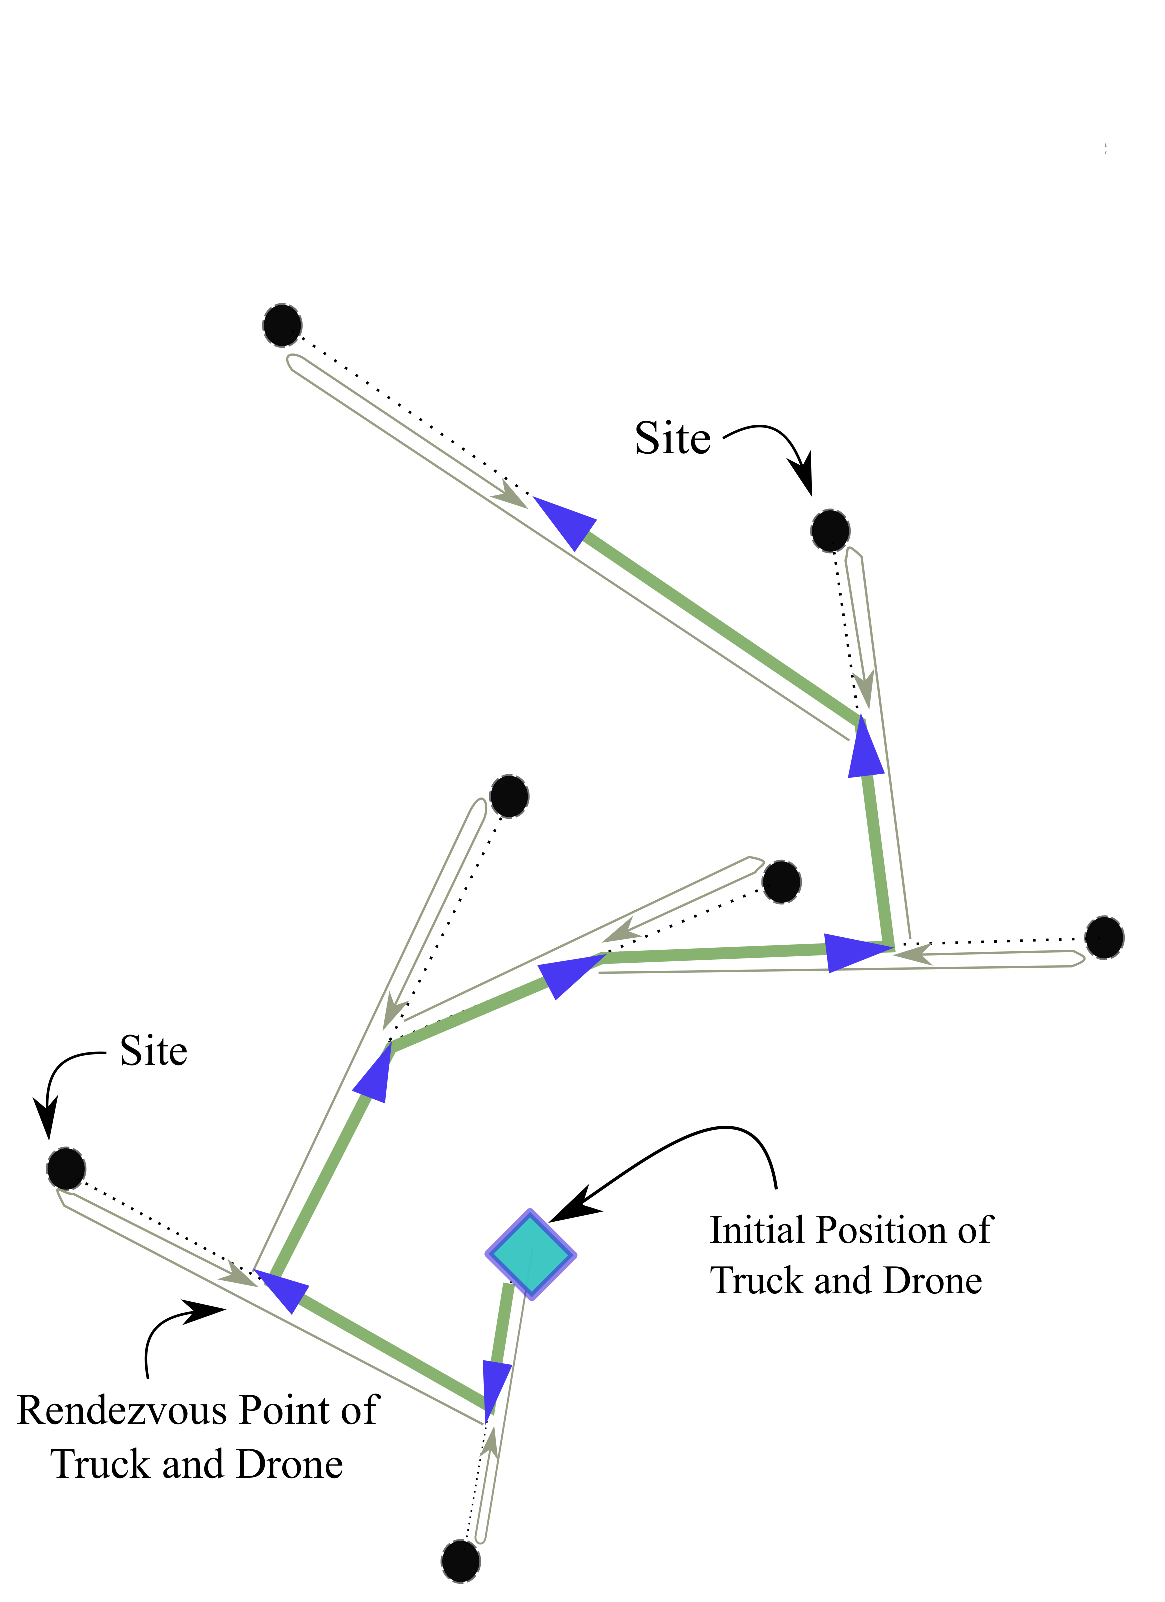
\includegraphics[width=7cm]{../webs/docs/collinear_horseflies.eps}
    \caption{The Collinear Horsefly Problem}
    \label{fig:collinear-horseflies}
\end{figure}

We can show that an optimal (unrestricted) horsfly solution can be converted
to a collinear-horsefly solution at a constant factor increase in the makespan. 

\subsection{Algorithmic Details}

\newchunk  
This implements the greedy algorithm for the canonical greedy
algorithm for collinear horsefly, and then uses the ordering 
obtained to get the exact tour for that given ordering.
Many variations on this are possible. However, this algorithm
is simple and may be more amenable to theoretical analysis. 
We will need an inequality for collapsing chains however. 

After extracting the ordering. we use exact/approximate solver for 
getting a horse-tour that is optimal/approximately optimal for the 
computed ordering of sites by greedy.

%{python-mode}%
\begin{flushleft} \small\label{scrap37}\raggedright\small
\NWtarget{nuweb28}{} $\langle\,${\itshape Algorithms for classic horsefly}\nobreak\ {\footnotesize {28}}$\,\rangle\equiv$
\vspace{-1ex}
\begin{list}{}{} \item
\mbox{}\verb@   @\\
\mbox{}\verb@def algo_greedy(sites, inithorseposn, phi, @\\
\mbox{}\verb@                write_algo_states_to_disk_p = True   ,@\\
\mbox{}\verb@                animate_schedule_p          = True   , @\\
\mbox{}\verb@                post_optimizer              = None):@\\
\mbox{}\verb@@\\
\mbox{}\verb@      @\hbox{$\langle\,${\itshape Set log, algo-state and input-output files config for \verb|algo_greedy|}\nobreak\ {\footnotesize \NWlink{nuweb29a}{29a}}$\,\rangle$}\verb@@\\
\mbox{}\verb@      @\hbox{$\langle\,${\itshape Define function \verb|next_rendezvous_point_for_horse_and_fly|}\nobreak\ {\footnotesize \NWlink{nuweb29b}{29b}}$\,\rangle$}\verb@@\\
\mbox{}\verb@      @\hbox{$\langle\,${\itshape Define function \verb|greedy|}\nobreak\ {\footnotesize \NWlink{nuweb30a}{30a}}$\,\rangle$}\verb@@\\
\mbox{}\verb@@\\
\mbox{}\verb@      sites1                  = sites[:]@\\
\mbox{}\verb@      sites_ordered_by_greedy = greedy(inithorseposn, remaining_sites=sites1)@\\
\mbox{}\verb@      answer                  = post_optimizer(sites_ordered_by_greedy, inithorseposn, phi)@\\
\mbox{}\verb@    @\\
\mbox{}\verb@      @\hbox{$\langle\,${\itshape Write input and output of \verb|algo_greedy| to file}\nobreak\ {\footnotesize \NWlink{nuweb30b}{30b}}$\,\rangle$}\verb@@\\
\mbox{}\verb@      @\hbox{$\langle\,${\itshape Make an animation of the schedule computed by \verb|algo_greedy|, if \verb|animate_schedule_p == True|}\nobreak\ {\footnotesize \NWlink{nuweb30c}{30c}}$\,\rangle$}\verb@@\\
\mbox{}\verb@      return answer@\\
\mbox{}\verb@@{\NWsep}
\end{list}
\vspace{-1.5ex}
\footnotesize
\begin{list}{}{\setlength{\itemsep}{-\parsep}\setlength{\itemindent}{-\leftmargin}}
\item \NWtxtMacroDefBy\ \NWlink{nuweb27}{27}\NWlink{nuweb28}{, 28}\NWlink{nuweb31a}{, 31a}\NWlink{nuweb32b}{, 32b}\NWlink{nuweb38a}{, 38a}\NWlink{nuweb51}{, 51}\NWlink{nuweb54}{, 54}\NWlink{nuweb56}{, 56}.
\item \NWtxtMacroRefIn\ \NWlink{nuweb20a}{20a}.
\item \NWtxtIdentsUsed\nobreak\  \verb@greedy@\nobreak\ \NWlink{nuweb30a}{30a}, \verb@write_algo_states_to_disk_p@\nobreak\ \NWlink{nuweb38a}{38a}.
\item{}
\end{list}
\vspace{4ex}
\end{flushleft}
%{/python-mode}%


%{python-mode}%
\begin{flushleft} \small\label{scrap38}\raggedright\small
\NWtarget{nuweb29a}{} $\langle\,${\itshape Set log, algo-state and input-output files config for \verb|algo_greedy|}\nobreak\ {\footnotesize {29a}}$\,\rangle\equiv$
\vspace{-1ex}
\begin{list}{}{} \item
\mbox{}\verb@  @\\
\mbox{}\verb@import sys, logging, datetime, os, errno@\\
\mbox{}\verb@@\\
\mbox{}\verb@algo_name     = 'algo-greedy-nearest-neighbor'@\\
\mbox{}\verb@time_stamp    = datetime.datetime.now().strftime('Day-%Y-%m-%d_ClockTime-%H:%M:%S')@\\
\mbox{}\verb@dir_name      = algo_name + '---' + time_stamp@\\
\mbox{}\verb@log_file_name = dir_name + '/' + 'run.log'@\\
\mbox{}\verb@io_file_name  = 'input_and_output.yml'@\\
\mbox{}\verb@@\\
\mbox{}\verb@# Create directory for writing data-files and logs to for @\\
\mbox{}\verb@# current run of this algorithm@\\
\mbox{}\verb@try:@\\
\mbox{}\verb@    os.makedirs(dir_name)@\\
\mbox{}\verb@except OSError as e:@\\
\mbox{}\verb@    if e.errno != errno.EEXIST:@\\
\mbox{}\verb@        raise@\\
\mbox{}\verb@@\\
\mbox{}\verb@logging.basicConfig( filename = log_file_name,@\\
\mbox{}\verb@                     level    = logging.DEBUG,@\\
\mbox{}\verb@                     format   = '%(asctime)s: %(levelname)s: %(message)s',@\\
\mbox{}\verb@                     filemode = 'w' )@\\
\mbox{}\verb@#logger = logging.getLogger()@\\
\mbox{}\verb@info("Started running greedy_nearest_neighbor for classic horsefly")@\\
\mbox{}\verb@@\\
\mbox{}\verb@algo_state_counter = 0 @\\
\mbox{}\verb@@{\NWsep}
\end{list}
\vspace{-1.5ex}
\footnotesize
\begin{list}{}{\setlength{\itemsep}{-\parsep}\setlength{\itemindent}{-\leftmargin}}
\item \NWtxtMacroRefIn\ \NWlink{nuweb28}{28}.
\item \NWtxtIdentsUsed\nobreak\  \verb@greedy@\nobreak\ \NWlink{nuweb30a}{30a}, \verb@logger@\nobreak\ \NWlink{nuweb38b}{38b}.
\item{}
\end{list}
\vspace{4ex}
\end{flushleft}
%{/python-mode}%


\needspace{5cm}
\vspace{-0.8cm} \newchunk   When there is a single site, the meeting point of horse and fly
can be computed exactly (A simple formula is trivial to derive too, which I do so later)/ 

Here I just use the exact solver for computing the horse tour when the ordering is given 
foir a single site. 

%{python-mode}%
\begin{flushleft} \small
\begin{minipage}{\linewidth}\label{scrap39}\raggedright\small
\NWtarget{nuweb29b}{} $\langle\,${\itshape Define function \verb|next_rendezvous_point_for_horse_and_fly|}\nobreak\ {\footnotesize {29b}}$\,\rangle\equiv$
\vspace{-1ex}
\begin{list}{}{} \item
\mbox{}\verb@   @\\
\mbox{}\verb@def next_rendezvous_point_for_horse_and_fly(horseposn, site):@\\
\mbox{}\verb@@\\
\mbox{}\verb@     horseflytour = algo_exact_given_specific_ordering([site], horseposn, phi)@\\
\mbox{}\verb@     return horseflytour['tour_points'][-1]@\\
\mbox{}\verb@@{\NWsep}
\end{list}
\vspace{-1.5ex}
\footnotesize
\begin{list}{}{\setlength{\itemsep}{-\parsep}\setlength{\itemindent}{-\leftmargin}}
\item \NWtxtMacroRefIn\ \NWlink{nuweb28}{28}.
\item \NWtxtIdentsUsed\nobreak\  \verb@algo_exact_given_specific_ordering@\nobreak\ \NWlink{nuweb31a}{31a}.
\item{}
\end{list}
\end{minipage}\vspace{4ex}
\end{flushleft}
%{/python-mode}%


\vspace{-0.8cm} \newchunk
Begin the recursion process where for a given initial
position of horse and fly and a given collection of sites
you find the nearst neighbor proceed according to segment
horsefly formula for just and one site, and for the new
position repeat the process for the remaining list of sites. 
The greedy approach can be extended to by finding the k
nearest neighbors, constructing the exact horsefly tour
there, at the exit point, you repeat by taking k nearest
neighbors and so on. 

For reference see this link on how nn queries are performed. 
\url{https://docs.scipy.org/doc/scipy/reference/generated/scipy.spatial.KDTree.query.html}
Warning this is inefficient!!! I am rebuilding the 
kd-tree at each step. Right now, I am only doing this 
for convenience.

The next site to get serviced by the drone and horse after they meet-up
is the one which is closest to the current position of the horse. 


%{python-mode}%
\begin{flushleft} \small
\begin{minipage}{\linewidth}\label{scrap40}\raggedright\small
\NWtarget{nuweb30a}{} $\langle\,${\itshape Define function \verb|greedy|}\nobreak\ {\footnotesize {30a}}$\,\rangle\equiv$
\vspace{-1ex}
\begin{list}{}{} \item
\mbox{}\verb@   @\\
\mbox{}\verb@def greedy(current_horse_posn, remaining_sites):@\\
\mbox{}\verb@@\\
\mbox{}\verb@    if len(remaining_sites) == 1:@\\
\mbox{}\verb@          return remaining_sites@\\
\mbox{}\verb@    else:@\\
\mbox{}\verb@          from scipy import spatial@\\
\mbox{}\verb@          tree          = spatial.KDTree(remaining_sites)@\\
\mbox{}\verb@          pts           = np.array([current_horse_posn])@\\
\mbox{}\verb@          query_result  = tree.query(pts)@\\
\mbox{}\verb@          next_site_idx = query_result[1][0]@\\
\mbox{}\verb@          next_site     = remaining_sites[next_site_idx]@\\
\mbox{}\verb@@\\
\mbox{}\verb@          next_horse_posn = next_rendezvous_point_for_horse_and_fly(current_horse_posn, next_site)@\\
\mbox{}\verb@          remaining_sites.pop(next_site_idx) # the pop method modifies the list in place. @\\
\mbox{}\verb@                 @\\
\mbox{}\verb@          return [next_site] + greedy(current_horse_posn = next_horse_posn, remaining_sites = remaining_sites)@\\
\mbox{}\verb@@{\NWsep}
\end{list}
\vspace{-1.5ex}
\footnotesize
\begin{list}{}{\setlength{\itemsep}{-\parsep}\setlength{\itemindent}{-\leftmargin}}
\item \NWtxtMacroRefIn\ \NWlink{nuweb28}{28}.
\item \NWtxtIdentsDefed\nobreak\  \verb@greedy@\nobreak\ \NWlink{nuweb28}{28}\NWlink{nuweb29a}{, 29a}\NWlink{nuweb38b}{, 38b}.
\item{}
\end{list}
\end{minipage}\vspace{4ex}
\end{flushleft}
%{/python-mode}%




\vspace{-0.8cm}\newchunk The final answer is written to disk in the form of a YAML file. It lists the input sites 
in the order of visitation computed by the algorithm and gives the tour of the horse. 
Note that the number of points on the horse's tour is 1 more than the number of given sites. 
%{python-mode}%
\begin{flushleft} \small\label{scrap41}\raggedright\small
\NWtarget{nuweb30b}{} $\langle\,${\itshape Write input and output of \verb|algo_greedy| to file}\nobreak\ {\footnotesize {30b}}$\,\rangle\equiv$
\vspace{-1ex}
\begin{list}{}{} \item
\mbox{}\verb@@\\
\mbox{}\verb@data = {'visited_sites'  : answer['site_ordering'] ,@\\
\mbox{}\verb@        'horse_tour'     : [inithorseposn] + answer['tour_points']   , @\\
\mbox{}\verb@        'phi'            : phi                     , @\\
\mbox{}\verb@        'inithorseposn'  : inithorseposn}@\\
\mbox{}\verb@@\\
\mbox{}\verb@import yaml@\\
\mbox{}\verb@with open(dir_name + '/' + io_file_name, 'w') as outfile:     yaml.dump( data, \@\\
\mbox{}\verb@                outfile, \@\\
\mbox{}\verb@                default_flow_style=False)@\\
\mbox{}\verb@debug("Dumped input and output to " + io_file_name)@\\
\mbox{}\verb@@{\NWsep}
\end{list}
\vspace{-1.5ex}
\footnotesize
\begin{list}{}{\setlength{\itemsep}{-\parsep}\setlength{\itemindent}{-\leftmargin}}
\item \NWtxtMacroRefIn\ \NWlink{nuweb28}{28}.
\item \NWtxtIdentsUsed\nobreak\  \verb@io_file_name,@\nobreak\ \NWlink{nuweb38b}{38b}.
\item{}
\end{list}
\vspace{4ex}
\end{flushleft}
%{/python-mode}%



\vspace{-0.8cm} \newchunk
%{python-mode}%
\begin{flushleft} \small
\begin{minipage}{\linewidth}\label{scrap42}\raggedright\small
\NWtarget{nuweb30c}{} $\langle\,${\itshape Make an animation of the schedule computed by \verb|algo_greedy|, if \verb|animate_schedule_p == True|}\nobreak\ {\footnotesize {30c}}$\,\rangle\equiv$
\vspace{-1ex}
\begin{list}{}{} \item
\mbox{}\verb@@\\
\mbox{}\verb@if animate_schedule_p : @\\
\mbox{}\verb@     animateSchedule(dir_name + '/' + io_file_name)@\\
\mbox{}\verb@@{\NWsep}
\end{list}
\vspace{-1.5ex}
\footnotesize
\begin{list}{}{\setlength{\itemsep}{-\parsep}\setlength{\itemindent}{-\leftmargin}}
\item \NWtxtMacroRefIn\ \NWlink{nuweb28}{28}.

\item{}
\end{list}
\end{minipage}\vspace{4ex}
\end{flushleft}
%{/python-mode}%










\vspace{-0.8cm} \newchunk Many of the heuristics, such as the two above that we just implemented, we compute an ordering of sites to visit
and then compute the tour-points for the horse. For a given order of visitation calcualting the horse-tour can be done by convex 
optimization. We give one such routine below, that uses the SLSQP non-linear solver from scipy for computing this horse-tour. I will 
implement the convex optimization routine from John's paper in a later section. Having two such independent routines for doing the same 
computation can help in benchmarking. 

Later, we will also study approximation algorithms for methods to compute horse-tours for a given order of visitation. For these I will need 
to benchmark the speed of solving SOCP's versus LP's to see what interesting questions can be studies in this regard. 

Since the horsely tour lies inside the square, the bounds for each coordinate for the initial guess is between 0 and 1. Many options 
are possible, Below I try two possibilities

\needspace{3cm}
%{python-mode}%
\begin{flushleft} \small\label{scrap43}\raggedright\small
\NWtarget{nuweb31a}{} $\langle\,${\itshape Algorithms for classic horsefly}\nobreak\ {\footnotesize {31a}}$\,\rangle\equiv$
\vspace{-1ex}
\begin{list}{}{} \item
\mbox{}\verb@def algo_exact_given_specific_ordering (sites, horseflyinit, phi):@\\
\mbox{}\verb@@\\
\mbox{}\verb@    @\hbox{$\langle\,${\itshape Useful functions for \verb|algo_exact_given_specific_ordering|}\nobreak\ {\footnotesize \NWlink{nuweb31b}{31b}, \ldots\ }$\,\rangle$}\verb@@\\
\mbox{}\verb@    @\\
\mbox{}\verb@    cons = generate_constraints(horseflyinit, phi, sites)@\\
\mbox{}\verb@    @\\
\mbox{}\verb@    # Initial guess for the non-linear solver.@\\
\mbox{}\verb@    #x0 = np.empty(2*len(sites)); x0.fill(0.5) # choice of filling vector with 0.5 is arbitrary@\\
\mbox{}\verb@    x0 = utils_algo.flatten_list_of_lists(sites) # the initial choice is just the sites@\\
\mbox{}\verb@@\\
\mbox{}\verb@    assert(len(x0) == 2*len(sites))@\\
\mbox{}\verb@@\\
\mbox{}\verb@    x0                  = np.array(x0)@\\
\mbox{}\verb@    sol                 = minimize(tour_length(horseflyinit), x0, method= 'SLSQP', \@\\
\mbox{}\verb@                                   constraints=cons         , options={'maxiter':500})@\\
\mbox{}\verb@    tour_points         = utils_algo.pointify_vector(sol.x)@\\
\mbox{}\verb@    numsites            = len(sites)@\\
\mbox{}\verb@    alpha               = horseflyinit[0]@\\
\mbox{}\verb@    beta                = horseflyinit[1]@\\
\mbox{}\verb@    s                   = utils_algo.flatten_list_of_lists(sites)@\\
\mbox{}\verb@    horse_waiting_times = np.zeros(numsites)@\\
\mbox{}\verb@    ps                  = sol.x@\\
\mbox{}\verb@@\\
\mbox{}\verb@    for i in range(numsites):@\\
\mbox{}\verb@@\\
\mbox{}\verb@        if i == 0 :@\\
\mbox{}\verb@            horse_time         = np.sqrt((ps[0]-alpha)**2 + (ps[1]-beta)**2)@\\
\mbox{}\verb@            fly_time_to_site   = 1.0/phi * np.sqrt((s[0]-alpha)**2 + (s[1]-beta)**2 )@\\
\mbox{}\verb@            fly_time_from_site = 1.0/phi * np.sqrt((s[0]-ps[1])**2 + (s[1]-ps[1])**2)@\\
\mbox{}\verb@        else:@\\
\mbox{}\verb@            horse_time         = np.sqrt((ps[2*i]-ps[2*i-2])**2 + (ps[2*i+1]-ps[2*i-1])**2)@\\
\mbox{}\verb@            fly_time_to_site   = 1.0/phi * np.sqrt(( (s[2*i]-ps[2*i-2])**2 + (s[2*i+1]-ps[2*i-1])**2 )) @\\
\mbox{}\verb@            fly_time_from_site = 1.0/phi * np.sqrt(( (s[2*i]-ps[2*i])**2   + (s[2*i+1]-ps[2*i+1])**2 )) @\\
\mbox{}\verb@@\\
\mbox{}\verb@        horse_waiting_times[i] = horse_time - (fly_time_to_site + fly_time_from_site)@\\
\mbox{}\verb@    @\\
\mbox{}\verb@    return {'tour_points'                : tour_points,@\\
\mbox{}\verb@            'horse_waiting_times'        : horse_waiting_times, @\\
\mbox{}\verb@            'site_ordering'              : sites,@\\
\mbox{}\verb@            'tour_length_with_waiting_time_included': \@\\
\mbox{}\verb@                                       tour_length_with_waiting_time_included(\@\\
\mbox{}\verb@                                                    tour_points, \@\\
\mbox{}\verb@                                                    horse_waiting_times, @\\
\mbox{}\verb@                                                    horseflyinit)}@\\
\mbox{}\verb@@{\NWsep}
\end{list}
\vspace{-1.5ex}
\footnotesize
\begin{list}{}{\setlength{\itemsep}{-\parsep}\setlength{\itemindent}{-\leftmargin}}
\item \NWtxtMacroDefBy\ \NWlink{nuweb27}{27}\NWlink{nuweb28}{, 28}\NWlink{nuweb31a}{, 31a}\NWlink{nuweb32b}{, 32b}\NWlink{nuweb38a}{, 38a}\NWlink{nuweb51}{, 51}\NWlink{nuweb54}{, 54}\NWlink{nuweb56}{, 56}.
\item \NWtxtMacroRefIn\ \NWlink{nuweb20a}{20a}.
\item \NWtxtIdentsDefed\nobreak\  \verb@algo_exact_given_specific_ordering@\nobreak\ \NWlink{nuweb22}{22}\NWlink{nuweb27}{, 27}\NWlink{nuweb29b}{, 29b}.\item \NWtxtIdentsUsed\nobreak\  \verb@generate_constraints@\nobreak\ \NWlink{nuweb32a}{32a}, \verb@tour_length@\nobreak\ \NWlink{nuweb57a}{57a}, \verb@tour_length_with_waiting_time_included@\nobreak\ \NWlink{nuweb57b}{57b}.
\item{}
\end{list}
\vspace{4ex}
\end{flushleft}
%{/python-mode}%



\vspace{-0.8cm} \newchunk For the ith segment of the horsefly tour this function returns a constraint function which 
models the fact that the time taken by the fly is equal to the time taken by the horse along that particular segment.

%{python-mode}%
\begin{flushleft} \small\label{scrap44}\raggedright\small
\NWtarget{nuweb31b}{} $\langle\,${\itshape Useful functions for \verb|algo_exact_given_specific_ordering|}\nobreak\ {\footnotesize {31b}}$\,\rangle\equiv$
\vspace{-1ex}
\begin{list}{}{} \item
\mbox{}\verb@@\\
\mbox{}\verb@def ith_leg_constraint(i, horseflyinit, phi, sites):@\\
\mbox{}\verb@        if i == 0 :@\\
\mbox{}\verb@            def _constraint_function(x):@\\
\mbox{}\verb@            @\\
\mbox{}\verb@                #print "Constraint  ", i@\\
\mbox{}\verb@                start = np.array (horseflyinit)@\\
\mbox{}\verb@                site  = np.array (sites[0])@\\
\mbox{}\verb@                stop  = np.array ([x[0],x[1]])@\\
\mbox{}\verb@            @\\
\mbox{}\verb@                horsetime = np.linalg.norm( stop - start )@\\
\mbox{}\verb@            @\\
\mbox{}\verb@                flytime_to_site   = 1/phi * np.linalg.norm( site - start )@\\
\mbox{}\verb@                flytime_from_site = 1/phi * np.linalg.norm( stop - site  )@\\
\mbox{}\verb@                flytime           = flytime_to_site + flytime_from_site@\\
\mbox{}\verb@                return horsetime-flytime@\\
\mbox{}\verb@@\\
\mbox{}\verb@            return _constraint_function@\\
\mbox{}\verb@        else :@\\
\mbox{}\verb@          @\\
\mbox{}\verb@            def _constraint_function(x):@\\
\mbox{}\verb@@\\
\mbox{}\verb@               #print "Constraint  ", i@\\
\mbox{}\verb@               start = np.array (  [x[2*i-2], x[2*i-1]]  ) @\\
\mbox{}\verb@               site  = np.array (  sites[i])@\\
\mbox{}\verb@               stop  = np.array (  [x[2*i]  , x[2*i+1]]  )@\\
\mbox{}\verb@            @\\
\mbox{}\verb@               horsetime = np.linalg.norm( stop - start )@\\
\mbox{}\verb@           @\\
\mbox{}\verb@               flytime_to_site   = 1/phi * np.linalg.norm( site - start )@\\
\mbox{}\verb@               flytime_from_site = 1/phi * np.linalg.norm( stop - site  )@\\
\mbox{}\verb@               flytime           = flytime_to_site + flytime_from_site@\\
\mbox{}\verb@               return horsetime-flytime@\\
\mbox{}\verb@@\\
\mbox{}\verb@            return _constraint_function@\\
\mbox{}\verb@@{\NWsep}
\end{list}
\vspace{-1.5ex}
\footnotesize
\begin{list}{}{\setlength{\itemsep}{-\parsep}\setlength{\itemindent}{-\leftmargin}}
\item \NWtxtMacroDefBy\ \NWlink{nuweb31b}{31b}\NWlink{nuweb32a}{, 32a}.
\item \NWtxtMacroRefIn\ \NWlink{nuweb31a}{31a}.
\item \NWtxtIdentsDefed\nobreak\  \verb@ith_leg_constraint@\nobreak\ \NWlink{nuweb32a}{32a}.
\item{}
\end{list}
\vspace{4ex}
\end{flushleft}
%{/python-mode}%

\vspace{-0.8cm} \newchunk Given input data, of the problem generate the constraint list for each leg 
of the tour. The number of legs is equal to the number of sites for the case of single horse, single drone
%{python-mode}%
\begin{flushleft} \small\label{scrap45}\raggedright\small
\NWtarget{nuweb32a}{} $\langle\,${\itshape Useful functions for \verb|algo_exact_given_specific_ordering|}\nobreak\ {\footnotesize {32a}}$\,\rangle\equiv$
\vspace{-1ex}
\begin{list}{}{} \item
\mbox{}\verb@@\\
\mbox{}\verb@def generate_constraints(horseflyinit, phi, sites):@\\
\mbox{}\verb@   cons = []@\\
\mbox{}\verb@   for i in range(len(sites)):@\\
\mbox{}\verb@        cons.append({'type':'eq','fun': ith_leg_constraint(i,horseflyinit,phi,sites)})@\\
\mbox{}\verb@   return cons@\\
\mbox{}\verb@@{\NWsep}
\end{list}
\vspace{-1.5ex}
\footnotesize
\begin{list}{}{\setlength{\itemsep}{-\parsep}\setlength{\itemindent}{-\leftmargin}}
\item \NWtxtMacroDefBy\ \NWlink{nuweb31b}{31b}\NWlink{nuweb32a}{, 32a}.
\item \NWtxtMacroRefIn\ \NWlink{nuweb31a}{31a}.
\item \NWtxtIdentsDefed\nobreak\  \verb@generate_constraints@\nobreak\ \NWlink{nuweb31a}{31a}\NWlink{nuweb54}{, 54}.\item \NWtxtIdentsUsed\nobreak\  \verb@ith_leg_constraint@\nobreak\ \NWlink{nuweb31b}{31b}.
\item{}
\end{list}
\vspace{4ex}
\end{flushleft}
%{/python-mode}%




\vspace{-0.8cm} \newchunk Another useful post-optimizer is one using the $L1$ metric and linear programming. 
This solves a Linear program using MOSEK and tries to solve the 
$L1$ version of the equations, with some modifications as outlined
    in the notebook.

The hope is that solving this is more scalable even if approximate
than using the SLSQP solver which chokes on >= 70-80 sites. 
    
I followed the MOSEK tutorial given here to set up the linear system
\url{https://docs.mosek.com/8.1/pythonapi/tutorial-lo-shared.html}
    
Note that MOSEK has been optimized to solve large \underline{sparse} systems of LPs. 
The LP that I set up here is extremely sparse! And hence a perfect fit 
for MOSEK. 


%{python-mode}%
\begin{flushleft} \small\label{scrap46}\raggedright\small
\NWtarget{nuweb32b}{} $\langle\,${\itshape Algorithms for classic horsefly}\nobreak\ {\footnotesize {32b}}$\,\rangle\equiv$
\vspace{-1ex}
\begin{list}{}{} \item
\mbox{}\verb@ @\\
\mbox{}\verb@def  algo_approximate_L1_given_specific_ordering(sites, horseflyinit, phi):@\\
\mbox{}\verb@    import mosek@\\
\mbox{}\verb@    numsites = len(sites)@\\
\mbox{}\verb@@\\
\mbox{}\verb@    def p(idx):@\\
\mbox{}\verb@        return idx + 0*numsites@\\
\mbox{}\verb@@\\
\mbox{}\verb@    def b(idx):@\\
\mbox{}\verb@        return idx + 2*numsites@\\
\mbox{}\verb@@\\
\mbox{}\verb@    def f(idx):@\\
\mbox{}\verb@        return idx + 4*numsites@\\
\mbox{}\verb@@\\
\mbox{}\verb@    def h(idx):@\\
\mbox{}\verb@        return idx + 6*numsites@\\
\mbox{}\verb@    @\\
\mbox{}\verb@    # Define a stream printer to grab output from MOSEK@\\
\mbox{}\verb@    def streamprinter(text):@\\
\mbox{}\verb@        sys.stdout.write(text)@\\
\mbox{}\verb@        sys.stdout.flush()@\\
\mbox{}\verb@@\\
\mbox{}\verb@    numcon = 9 + 13*(numsites-1) # the first site has 9 constraints while the remaining n-1 sites have 13 constraints each@\\
\mbox{}\verb@    numvar = 8 * numsites # Each ``L1 triangle'' has 8 variables associated with it@\\
\mbox{}\verb@@\\
\mbox{}\verb@    alpha = horseflyinit[0]@\\
\mbox{}\verb@    beta  = horseflyinit[1]@\\
\mbox{}\verb@@\\
\mbox{}\verb@    s = utils_algo.flatten_list_of_lists(sites)@\\
\mbox{}\verb@@\\
\mbox{}\verb@    # Make mosek environment@\\
\mbox{}\verb@    with mosek.Env() as env:@\\
\mbox{}\verb@        # Create a task object@\\
\mbox{}\verb@        with env.Task(0, 0) as task:@\\
\mbox{}\verb@            # Attach a log stream printer to the task@\\
\mbox{}\verb@            task.set_Stream(mosek.streamtype.log, streamprinter)@\\
\mbox{}\verb@            # Append 'numcon' empty constraints.@\\
\mbox{}\verb@            # The constraints will initially have no bounds.@\\
\mbox{}\verb@            task.appendcons(numcon)@\\
\mbox{}\verb@            # Append 'numvar' variables.@\\
\mbox{}\verb@            # The variables will initially be fixed at zero (x=0).@\\
\mbox{}\verb@            task.appendvars(numvar)@\\
\mbox{}\verb@@\\
\mbox{}\verb@            for idx in range(numvar):@\\
\mbox{}\verb@                if (0   <= idx) and (idx < 2*numsites): # free variables (p section of the vector)@\\
\mbox{}\verb@                    task.putvarbound(idx, mosek.boundkey.fr, -np.inf, np.inf)@\\
\mbox{}\verb@                    @\\
\mbox{}\verb@                elif  idx == 2*numsites : # b_0 is a known variable@\\
\mbox{}\verb@                    val = abs(s[0]-alpha)@\\
\mbox{}\verb@                    task.putvarbound(idx, mosek.boundkey.fx, val, val)@\\
\mbox{}\verb@                @\\
\mbox{}\verb@                elif  idx == 2*numsites +1 : # b_1 is a known variable@\\
\mbox{}\verb@                    val = abs(s[1]-beta)@\\
\mbox{}\verb@                    task.putvarbound(idx, mosek.boundkey.fx, val, val)@\\
\mbox{}\verb@@\\
\mbox{}\verb@                else : # b_2, onwards and the f and h sections of the vector@\\
\mbox{}\verb@                    task.putvarbound(idx, mosek.boundkey.lo, 0.0, np.inf)@\\
\mbox{}\verb@                    @\\
\mbox{}\verb@            # All the coefficients corresponding to the h's are 1's@\\
\mbox{}\verb@            # and for the others the coefficients are 0. @\\
\mbox{}\verb@            for i in range(numvar):@\\
\mbox{}\verb@                if i >= 6*numsites: # the h-section@\\
\mbox{}\verb@                    task.putcj(i,1)@\\
\mbox{}\verb@                else: # the p,b,f sections of x@\\
\mbox{}\verb@                    task.putcj(i,0)@\\
\mbox{}\verb@@\\
\mbox{}\verb@            # Constraints for the zeroth triangle corresponding to the zeroth site@\\
\mbox{}\verb@            row = -1@\\
\mbox{}\verb@            row += 1; task.putconbound(row, mosek.boundkey.up, -np.inf, alpha ) ; task.putarow(row, [p(0), h(0)],[1.0, -1.0])@\\
\mbox{}\verb@            row += 1; task.putconbound(row, mosek.boundkey.lo, alpha  , np.inf) ; task.putarow(row, [p(0), h(0)],[1.0,  1.0])@\\
\mbox{}\verb@@\\
\mbox{}\verb@            row += 1; task.putconbound(row, mosek.boundkey.up, -np.inf, beta ) ; task.putarow(row, [p(1), h(1)],[1.0, -1.0])@\\
\mbox{}\verb@            row += 1; task.putconbound(row, mosek.boundkey.lo, beta  , np.inf) ; task.putarow(row, [p(1), h(1)],[1.0,  1.0])@\\
\mbox{}\verb@            @\\
\mbox{}\verb@            row += 1; task.putconbound(row, mosek.boundkey.up, -np.inf, s[0]  ) ; task.putarow(row, [p(0), f(0)],[1.0, -1.0])@\\
\mbox{}\verb@            row += 1; task.putconbound(row, mosek.boundkey.lo,  s[0]  , np.inf) ; task.putarow(row, [p(0), f(0)],[1.0,  1.0])@\\
\mbox{}\verb@@\\
\mbox{}\verb@            row += 1; task.putconbound(row, mosek.boundkey.up, -np.inf, s[1]  ) ; task.putarow(row, [p(1), f(1)],[1.0, -1.0])@\\
\mbox{}\verb@            row += 1; task.putconbound(row, mosek.boundkey.lo,  s[1]  , np.inf) ; task.putarow(row, [p(1), f(1)],[1.0,  1.0])@\\
\mbox{}\verb@@\\
\mbox{}\verb@            # The most important constraint of all! On the ``L1 triangle''@\\
\mbox{}\verb@            # time for drone to start from the truck reach site and get back to truck@\\
\mbox{}\verb@            # = time for truck between the two successive rendezvous points@\\
\mbox{}\verb@            # The way I have modelled the following constraint it is not exactly@\\
\mbox{}\verb@            # the same as the previous statement of equality of times of truck@\\
\mbox{}\verb@            # and drone, but for initial experiments it looks like this gives@\\
\mbox{}\verb@            # waiting times to be automatically close to 0 (1e-9 close to machine-epsilon)@\\
\mbox{}\verb@            # Theorem in the making?? @\\
\mbox{}\verb@            row += 1; task.putconbound(row, mosek.boundkey.fx, 0.0 , 0.0 ) ;@\\
\mbox{}\verb@            task.putarow(row, [b(0), b(1), f(0), f(1), h(0), h(1)], [1.0,1.0,1.0,1.0,-phi, -phi])@\\
\mbox{}\verb@@\\
\mbox{}\verb@            # Constraints beginning from the 1st triangle@\\
\mbox{}\verb@            for  i in range(1,numsites):@\\
\mbox{}\verb@                row+=1 ;  task.putconbound(row, mosek.boundkey.lo, -s[2*i]  , np.inf) ; task.putarow(row, [b(2*i),   p(2*i-2)],[1.0, -1.0])@\\
\mbox{}\verb@                row+=1 ;  task.putconbound(row, mosek.boundkey.lo,  s[2*i]  , np.inf) ; task.putarow(row, [b(2*i),   p(2*i-2)],[1.0,  1.0])@\\
\mbox{}\verb@                row+=1 ;  task.putconbound(row, mosek.boundkey.lo, -s[2*i+1], np.inf) ; task.putarow(row, [b(2*i+1), p(2*i-1)],[1.0, -1.0])@\\
\mbox{}\verb@                row+=1 ;  task.putconbound(row, mosek.boundkey.lo,  s[2*i+1], np.inf) ; task.putarow(row, [b(2*i+1), p(2*i-1)],[1.0,  1.0])@\\
\mbox{}\verb@                @\\
\mbox{}\verb@                row+=1 ;  task.putconbound(row, mosek.boundkey.lo, -s[2*i]  , np.inf) ; task.putarow(row, [f(2*i),    p(2*i)]  ,[1.0, -1.0])@\\
\mbox{}\verb@                row+=1 ;  task.putconbound(row, mosek.boundkey.lo,  s[2*i]  , np.inf) ; task.putarow(row, [f(2*i),    p(2*i)]  ,[1.0,  1.0])@\\
\mbox{}\verb@                row+=1 ;  task.putconbound(row, mosek.boundkey.lo, -s[2*i+1], np.inf) ; task.putarow(row, [f(2*i+1),  p(2*i+1)],[1.0, -1.0])@\\
\mbox{}\verb@                row+=1 ;  task.putconbound(row, mosek.boundkey.lo,  s[2*i+1], np.inf) ; task.putarow(row, [f(2*i+1),  p(2*i+1)],[1.0,  1.0])@\\
\mbox{}\verb@                @\\
\mbox{}\verb@                row+=1 ;  task.putconbound(row, mosek.boundkey.lo, 0.0     , np.inf); task.putarow(row, [p(2*i)  , p(2*i-2), h(2*i)]  , [1.0,-1.0, 1.0])@\\
\mbox{}\verb@                row+=1 ;  task.putconbound(row, mosek.boundkey.up, -np.inf , 0.0   ); task.putarow(row, [p(2*i)  , p(2*i-2), h(2*i)]  , [1.0,-1.0,-1.0])@\\
\mbox{}\verb@                row+=1 ;  task.putconbound(row, mosek.boundkey.lo, 0.0     , np.inf); task.putarow(row, [p(2*i+1), p(2*i-1), h(2*i+1)], [1.0,-1.0, 1.0])@\\
\mbox{}\verb@                row+=1 ;  task.putconbound(row, mosek.boundkey.up, -np.inf , 0.0   ); task.putarow(row, [p(2*i+1), p(2*i-1), h(2*i+1)], [1.0,-1.0,-1.0])@\\
\mbox{}\verb@                # The most important constraint of all! On the ``L1 triangle''@\\
\mbox{}\verb@                # time for drone to start from the truck reach site and get back to truck@\\
\mbox{}\verb@                # = time for truck between the two successive rendezvous points@\\
\mbox{}\verb@                row+=1; task.putconbound(row, mosek.boundkey.fx, 0.0 , 0.0 ) ;@\\
\mbox{}\verb@                task.putarow(row, [b(2*i), b(2*i+1), f(2*i), f(2*i+1), h(2*i), h(2*i+1)], [1.0,1.0,1.0,1.0,-phi, -phi])@\\
\mbox{}\verb@@\\
\mbox{}\verb@            # Input the objective sense (minimize/maximize)@\\
\mbox{}\verb@            task.putobjsense(mosek.objsense.minimize)@\\
\mbox{}\verb@            task.optimize()@\\
\mbox{}\verb@            # Print a summary containing information@\\
\mbox{}\verb@            # about the solution for debugging purposes@\\
\mbox{}\verb@            #task.solutionsummary(mosek.streamtype.msg)@\\
\mbox{}\verb@@\\
\mbox{}\verb@            # Get status information about the solution@\\
\mbox{}\verb@            solsta = task.getsolsta(mosek.soltype.bas)@\\
\mbox{}\verb@            @\\
\mbox{}\verb@            if (solsta == mosek.solsta.optimal or@\\
\mbox{}\verb@                        solsta == mosek.solsta.near_optimal):@\\
\mbox{}\verb@                    xx = [0.] * numvar@\\
\mbox{}\verb@                        # Request the basic solution.@\\
\mbox{}\verb@                    task.getxx(mosek.soltype.bas, xx)@\\
\mbox{}\verb@                    #print("Optimal solution: ")@\\
\mbox{}\verb@                    #for i in range(numvar):@\\
\mbox{}\verb@                    #    print("x[" + str(i) + "]=" + str(xx[i]))@\\
\mbox{}\verb@            elif (solsta == mosek.solsta.dual_infeas_cer or@\\
\mbox{}\verb@                    solsta == mosek.solsta.prim_infeas_cer or@\\
\mbox{}\verb@                    solsta == mosek.solsta.near_dual_infeas_cer or@\\
\mbox{}\verb@                    solsta == mosek.solsta.near_prim_infeas_cer):@\\
\mbox{}\verb@                    print("Primal or dual infeasibility certificate found.\n")@\\
\mbox{}\verb@            elif solsta == mosek.solsta.unknown:@\\
\mbox{}\verb@                    print("Unknown solution status")@\\
\mbox{}\verb@            else:@\\
\mbox{}\verb@                    print("Other solution status")@\\
\mbox{}\verb@@\\
\mbox{}\verb@            # Now that we have solved the LP@\\
\mbox{}\verb@            # We need to extract the ``p'' section of the vector@\\
\mbox{}\verb@            ps = xx[:2*numsites]@\\
\mbox{}\verb@            bs = xx[2*numsites:4*numsites]@\\
\mbox{}\verb@            fs = xx[4*numsites:6*numsites]@\\
\mbox{}\verb@            hs = xx[6*numsites:]@\\
\mbox{}\verb@@\\
\mbox{}\verb@            ######################################################################################@\\
\mbox{}\verb@            # This commented out section is important to check how close to zero the waiting times@\\
\mbox{}\verb@            # are as calculated by the LP. To understand this, comment in this section and comment@\\
\mbox{}\verb@            # out the part using tghe L2 metric below it@\\
\mbox{}\verb@            ######################################################################################@\\
\mbox{}\verb@            # horse_waiting_times = np.zeros(numsites)@\\
\mbox{}\verb@            # for i in range(numsites):@\\
\mbox{}\verb@            #     if i == 0 :@\\
\mbox{}\verb@            #         horse_time         = abs(ps[0]-alpha) + abs(ps[1]-beta)@\\
\mbox{}\verb@            #         fly_time_to_site   = 1.0/phi * (abs(s[0]-alpha) + abs(s[1]-beta))@\\
\mbox{}\verb@            #         fly_time_from_site = 1.0/phi * (abs(s[0]-ps[1]) + abs(s[1]-ps[1]))@\\
\mbox{}\verb@            #     else:@\\
\mbox{}\verb@            #         horse_time         = abs(ps[2*i]-ps[2*i-2]) + abs(ps[2*i+1]-ps[2*i-1])@\\
\mbox{}\verb@            #         fly_time_to_site   = 1.0/phi * ( abs(s[2*i]-ps[2*i-2]) + abs(s[2*i+1]-ps[2*i-1]) ) @\\
\mbox{}\verb@            #         fly_time_from_site = 1.0/phi * ( abs(s[2*i]-ps[2*i])   + abs(s[2*i+1]-ps[2*i+1]) ) @\\
\mbox{}\verb@            #     horse_waiting_times[i] = horse_time - (fly_time_to_site + fly_time_from_site)@\\
\mbox{}\verb@@\\
\mbox{}\verb@            horse_waiting_times = np.zeros(numsites)@\\
\mbox{}\verb@            for i in range(numsites):@\\
\mbox{}\verb@                if i == 0 :@\\
\mbox{}\verb@                    horse_time         = np.sqrt((ps[0]-alpha)**2 + (ps[1]-beta)**2)@\\
\mbox{}\verb@                    fly_time_to_site   = 1.0/phi * np.sqrt((s[0]-alpha)**2 + (s[1]-beta)**2)@\\
\mbox{}\verb@                    fly_time_from_site = 1.0/phi * np.sqrt((s[0]-ps[1])**2 + (s[1]-ps[1])**2)@\\
\mbox{}\verb@                else:@\\
\mbox{}\verb@                    horse_time         = np.sqrt((ps[2*i]-ps[2*i-2])**2 + (ps[2*i+1]-ps[2*i-1])**2)@\\
\mbox{}\verb@                    fly_time_to_site   = 1.0/phi * np.sqrt( (s[2*i]-ps[2*i-2])**2 + (s[2*i+1]-ps[2*i-1])**2 ) @\\
\mbox{}\verb@                    fly_time_from_site = 1.0/phi * np.sqrt( (s[2*i]-ps[2*i])**2   + (s[2*i+1]-ps[2*i+1])**2 ) @\\
\mbox{}\verb@                    @\\
\mbox{}\verb@                horse_waiting_times[i] = horse_time - (fly_time_to_site + fly_time_from_site)@\\
\mbox{}\verb@                @\\
\mbox{}\verb@            tour_points = utils_algo.pointify_vector(ps)@\\
\mbox{}\verb@            return {'tour_points'        : tour_points,@\\
\mbox{}\verb@                    'horse_waiting_times': horse_waiting_times, @\\
\mbox{}\verb@                    'site_ordering'      : sites,@\\
\mbox{}\verb@                    'tour_length_with_waiting_time_included': tour_length_with_waiting_time_included(tour_points, horse_waiting_times, horseflyinit)}@\\
\mbox{}\verb@@\\
\mbox{}\verb@ @\\
\mbox{}\verb@@{\NWsep}
\end{list}
\vspace{-1.5ex}
\footnotesize
\begin{list}{}{\setlength{\itemsep}{-\parsep}\setlength{\itemindent}{-\leftmargin}}
\item \NWtxtMacroDefBy\ \NWlink{nuweb27}{27}\NWlink{nuweb28}{, 28}\NWlink{nuweb31a}{, 31a}\NWlink{nuweb32b}{, 32b}\NWlink{nuweb38a}{, 38a}\NWlink{nuweb51}{, 51}\NWlink{nuweb54}{, 54}\NWlink{nuweb56}{, 56}.
\item \NWtxtMacroRefIn\ \NWlink{nuweb20a}{20a}.
\item \NWtxtIdentsUsed\nobreak\  \verb@tour_length_with_waiting_time_included@\nobreak\ \NWlink{nuweb57b}{57b}.
\item{}
\end{list}
\vspace{4ex}
\end{flushleft}
%{/python-mode}%
\section{\framebox{Algorithm}: Greedy---Incremental Insertion}
\subsection*{Algorithmic Overview}
\newchunk The greedy nearest neighbor heuristic described in \autoref{sec:greedy-nn} gives an $O(\log n)$ 
          approximation for $n$ sites in the plane. However, there exists an alternative greedy incremental 
          insertion algorithm for the TSP that yields a 2-approximation. Similar to the greedy-nn algorithm 
          we can generalize the greedy-incremental approach to the collinear-horseflies setting 
          (cf: \autoref{fig:collinear-horseflies}). 

\newchunk In this approach, we maintain a list of visited sites $V$ (along with the order of visitation 
          $\mathcal{O}$) and the unvisited sites $U$. For the given collinear-horsefly tour serving $V$ 
          pick a site $s$ from $U$ along with a position in $\mathcal{O}$ (calling the resulting ordering  
          $\mathcal{O^{'}}$  ) that minimizes the cost of the horsefly tour serving the sites $V \cup \{s\}$ 
          in the order $\mathcal{O^{'}}$. 

% \begin{figure}[H]
% \centering
% 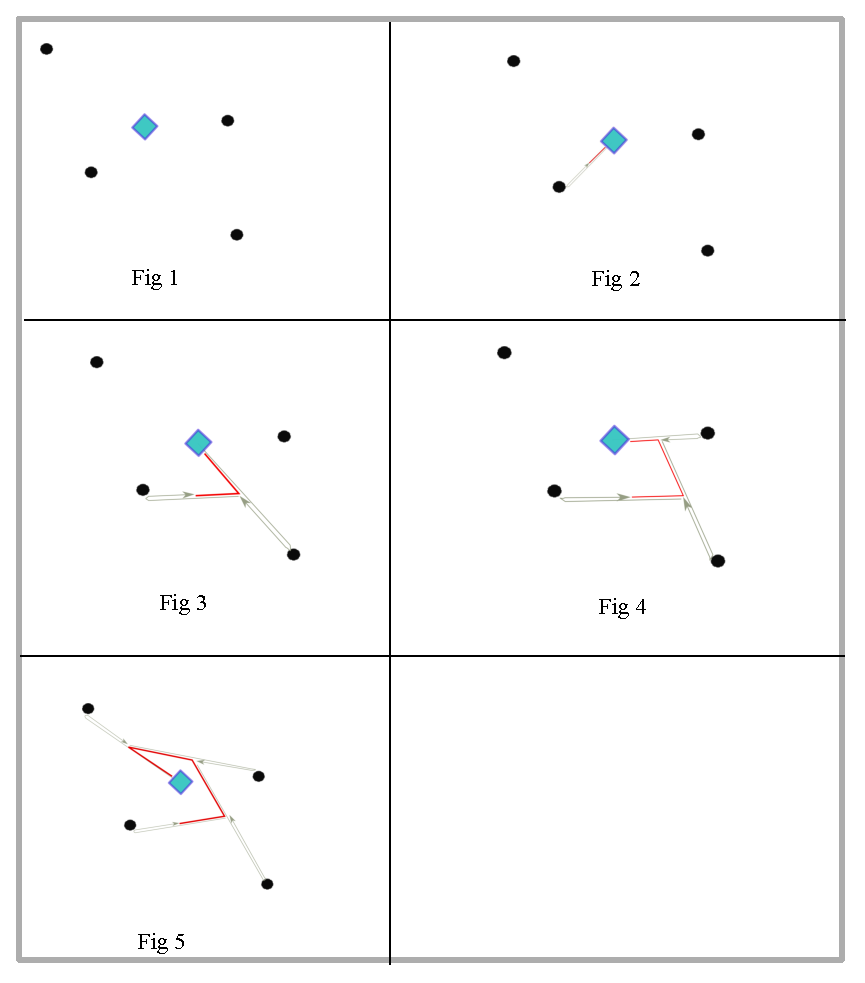
\includegraphics[width=8cm]{../webs/docs/incremental_insertion_frames.eps}
% \end{figure}

\begin{figure}[H]
\centering
\begin{tabular}{cc}
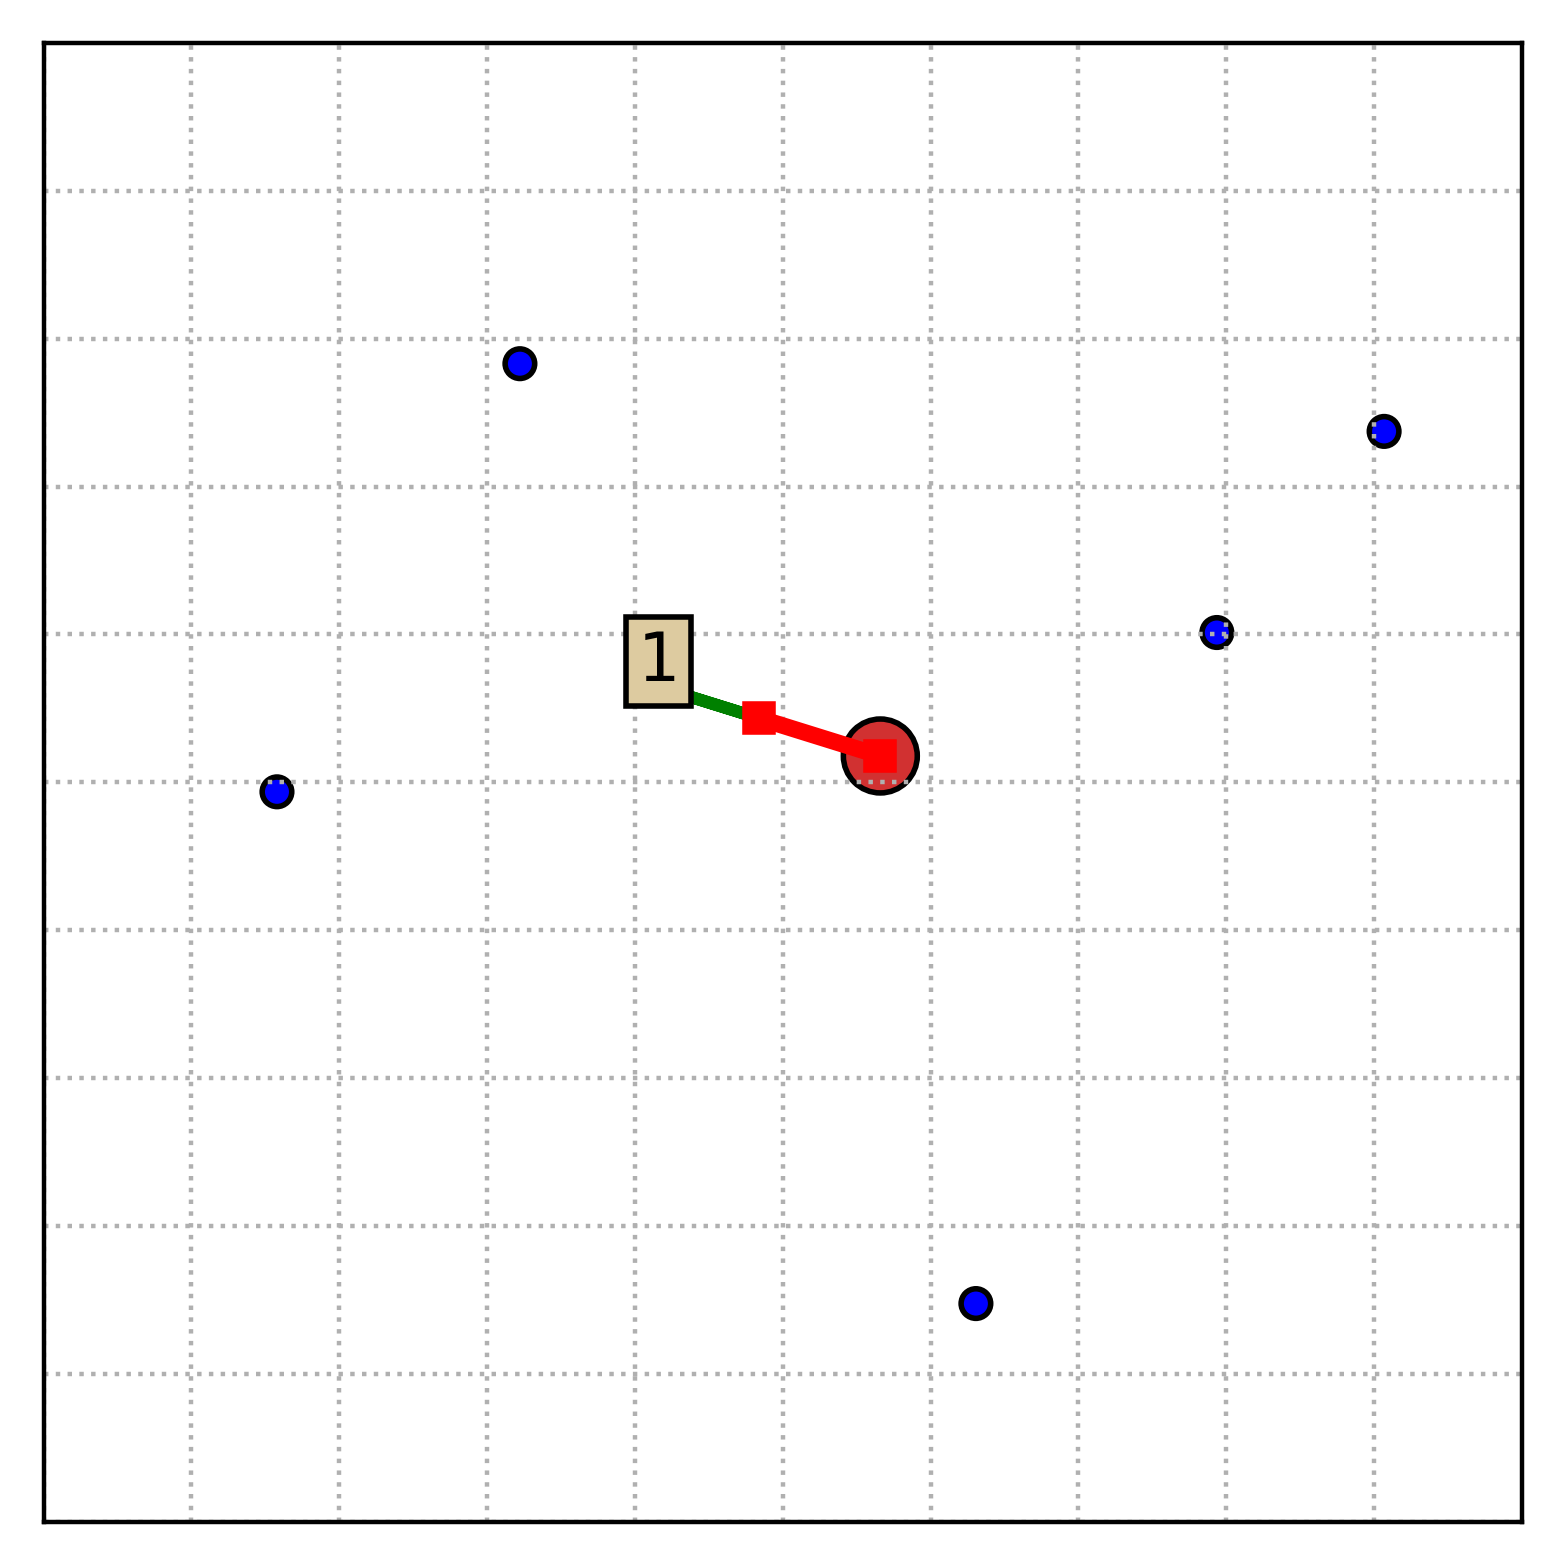
\includegraphics[width=8cm]{../webs/docs/algo-greedy-incremental-insertion---Day-2018-12-24_ClockTime-19:31:02/algo_state_00000.png}&
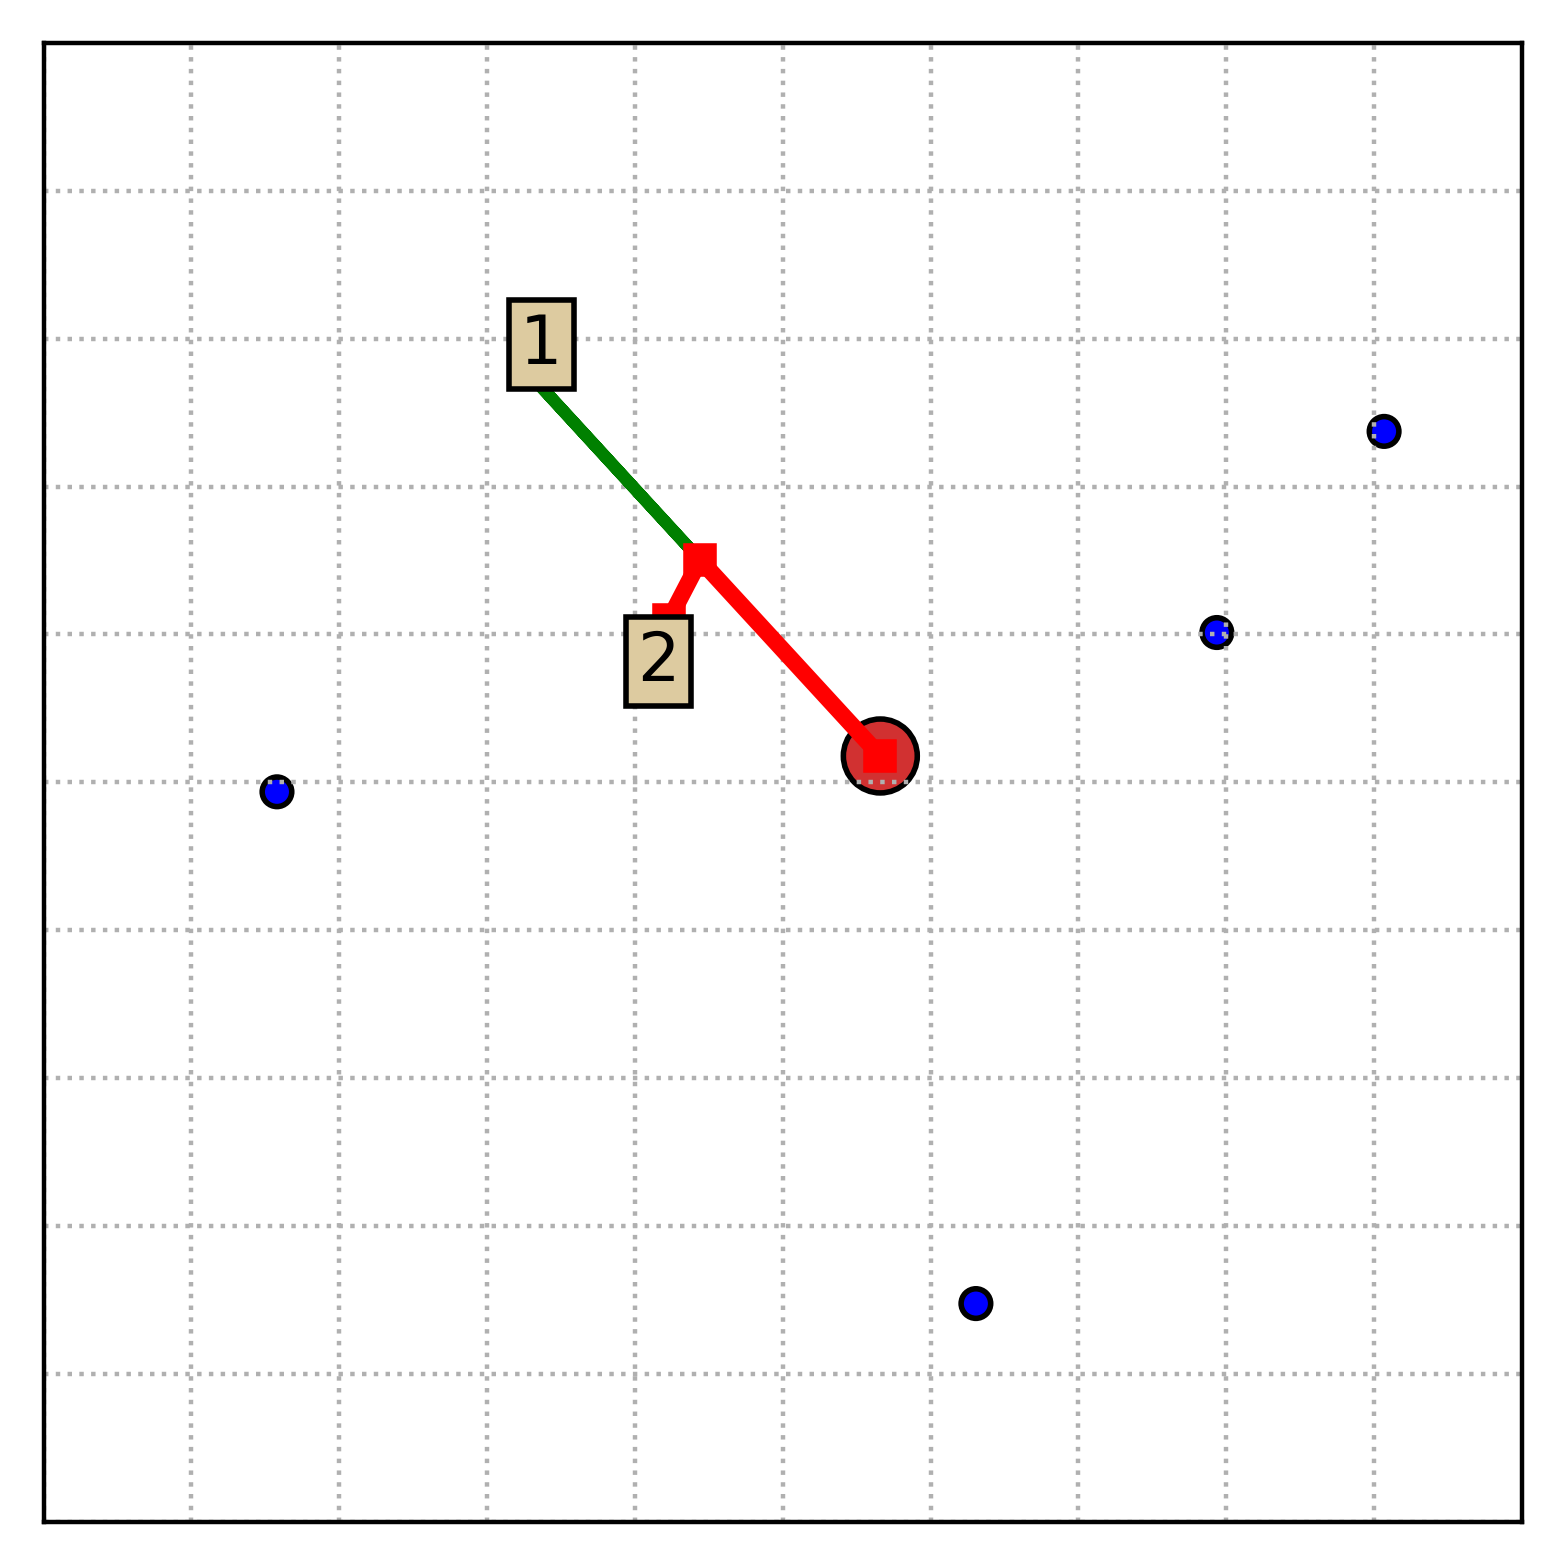
\includegraphics[width=8cm]{../webs/docs/algo-greedy-incremental-insertion---Day-2018-12-24_ClockTime-19:31:02/algo_state_00001.png}\\
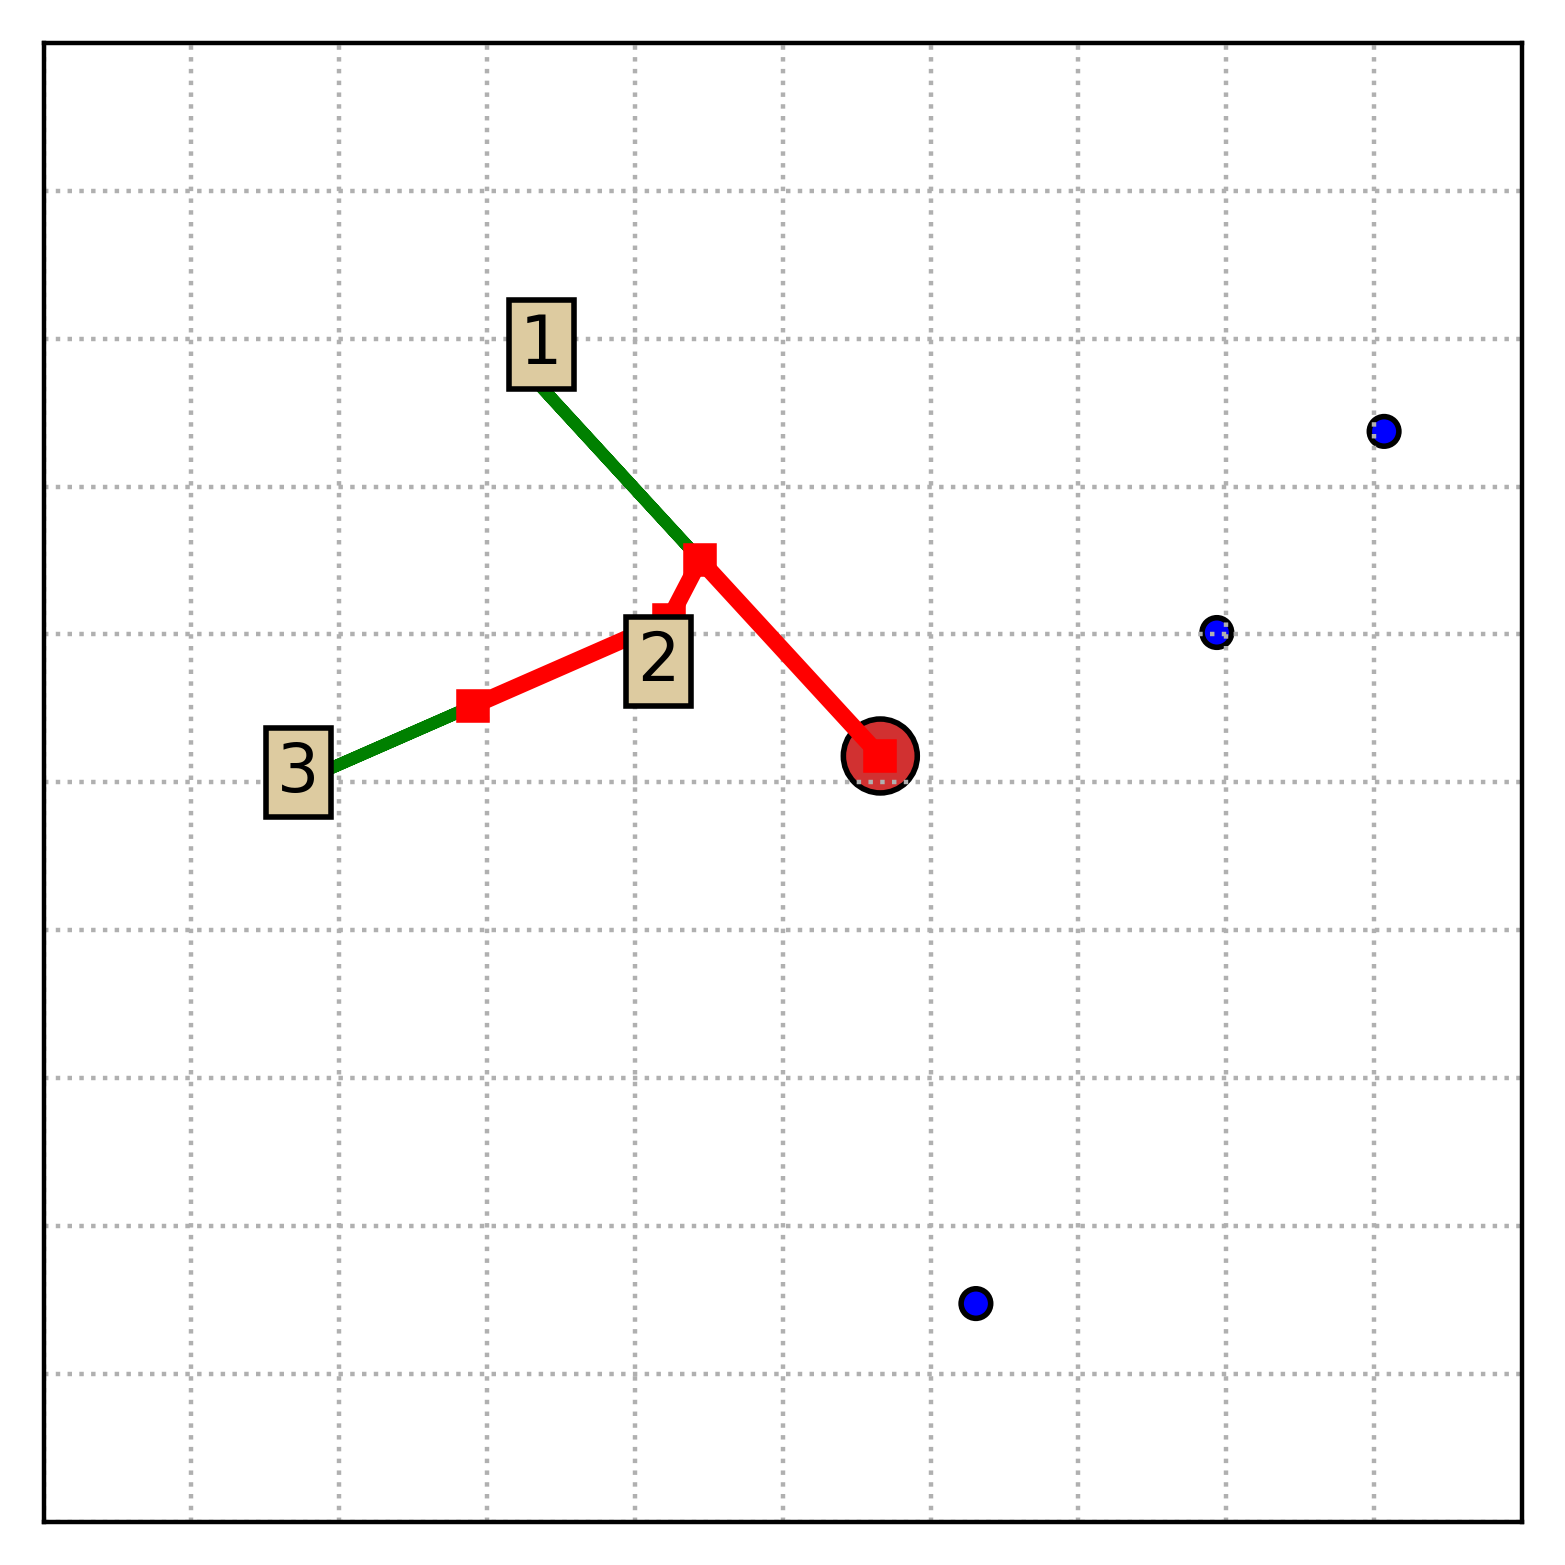
\includegraphics[width=8cm]{../webs/docs/algo-greedy-incremental-insertion---Day-2018-12-24_ClockTime-19:31:02/algo_state_00002.png}&
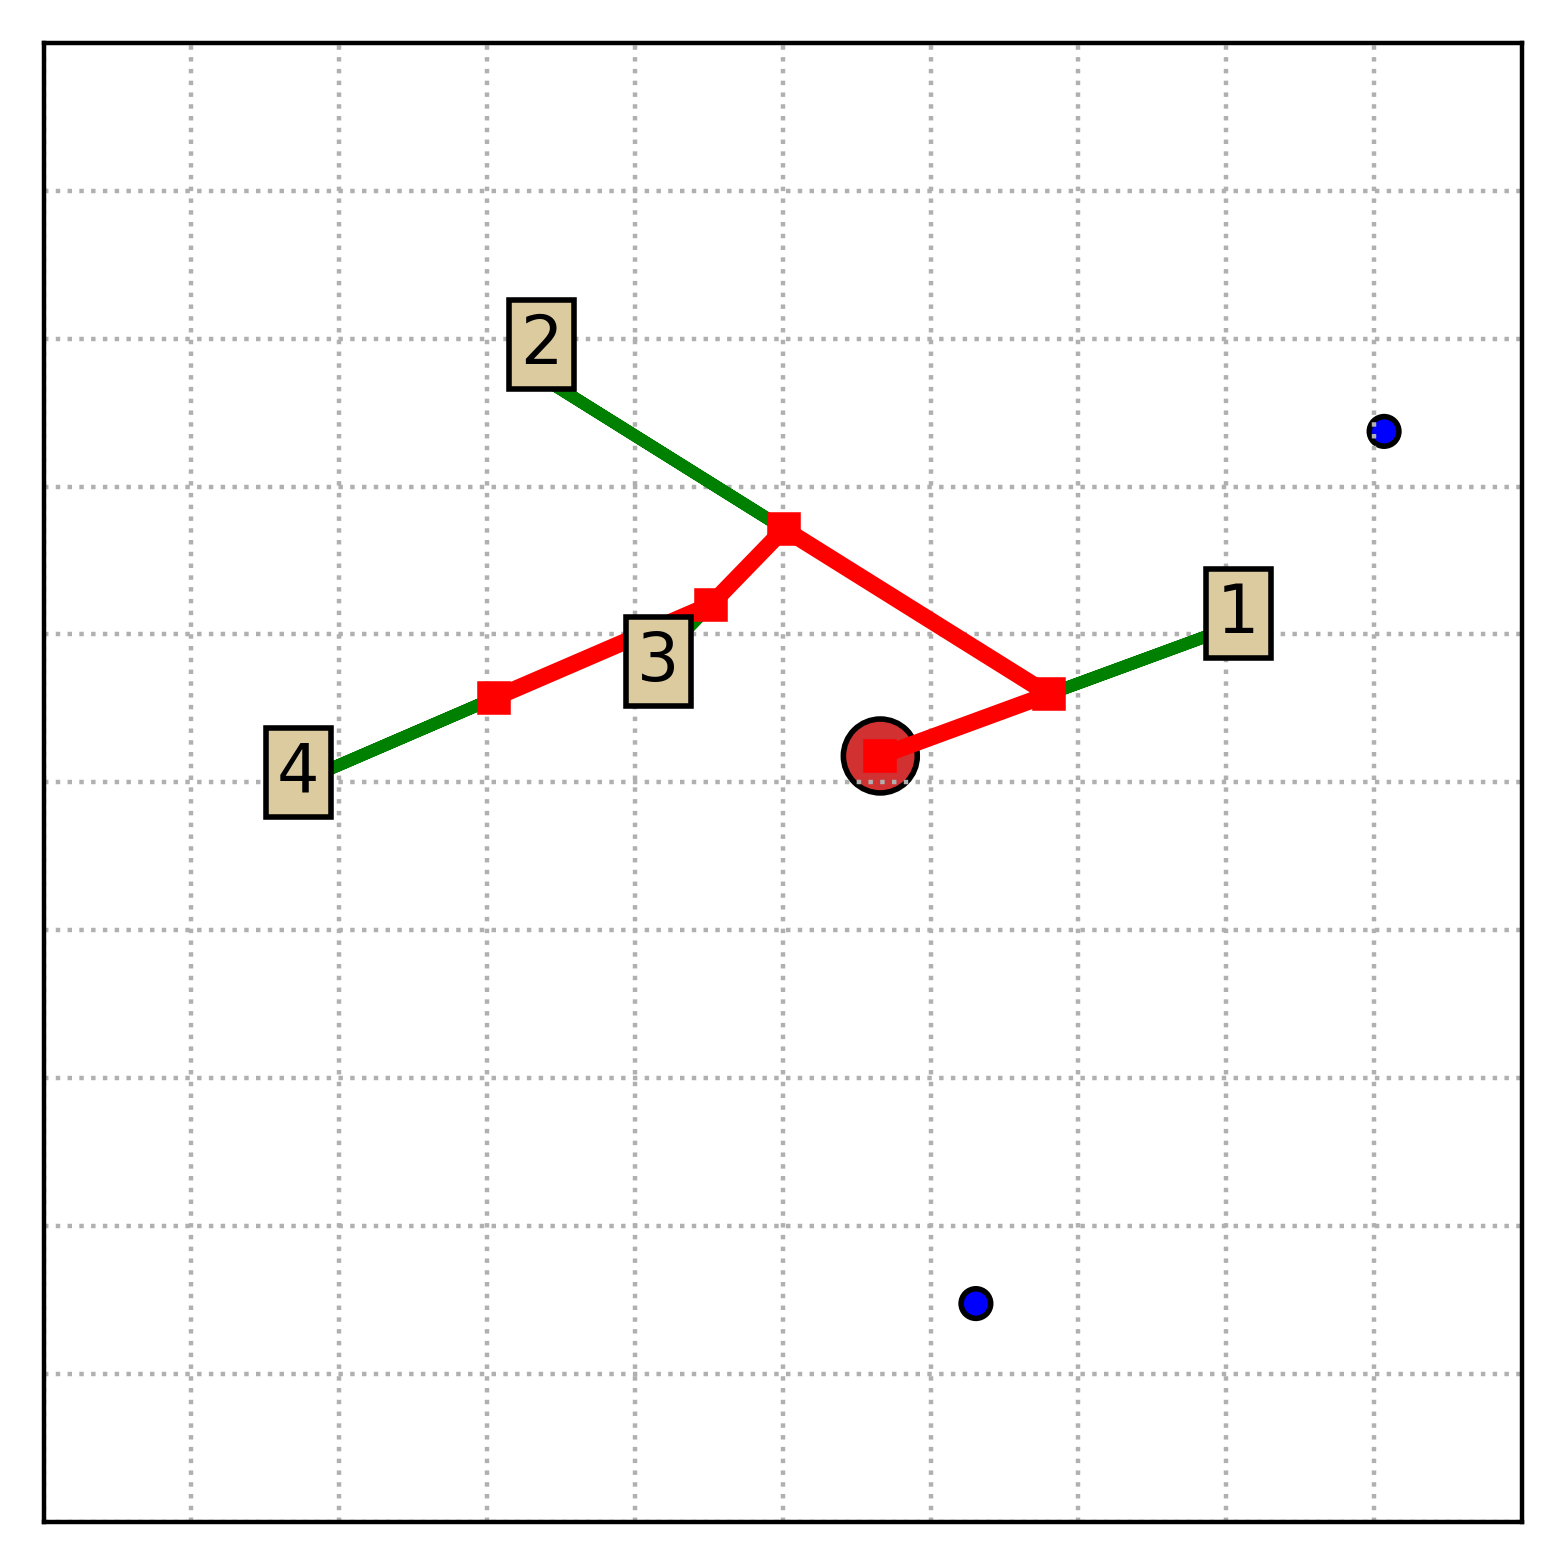
\includegraphics[width=8cm]{../webs/docs/algo-greedy-incremental-insertion---Day-2018-12-24_ClockTime-19:31:02/algo_state_00003.png}\\
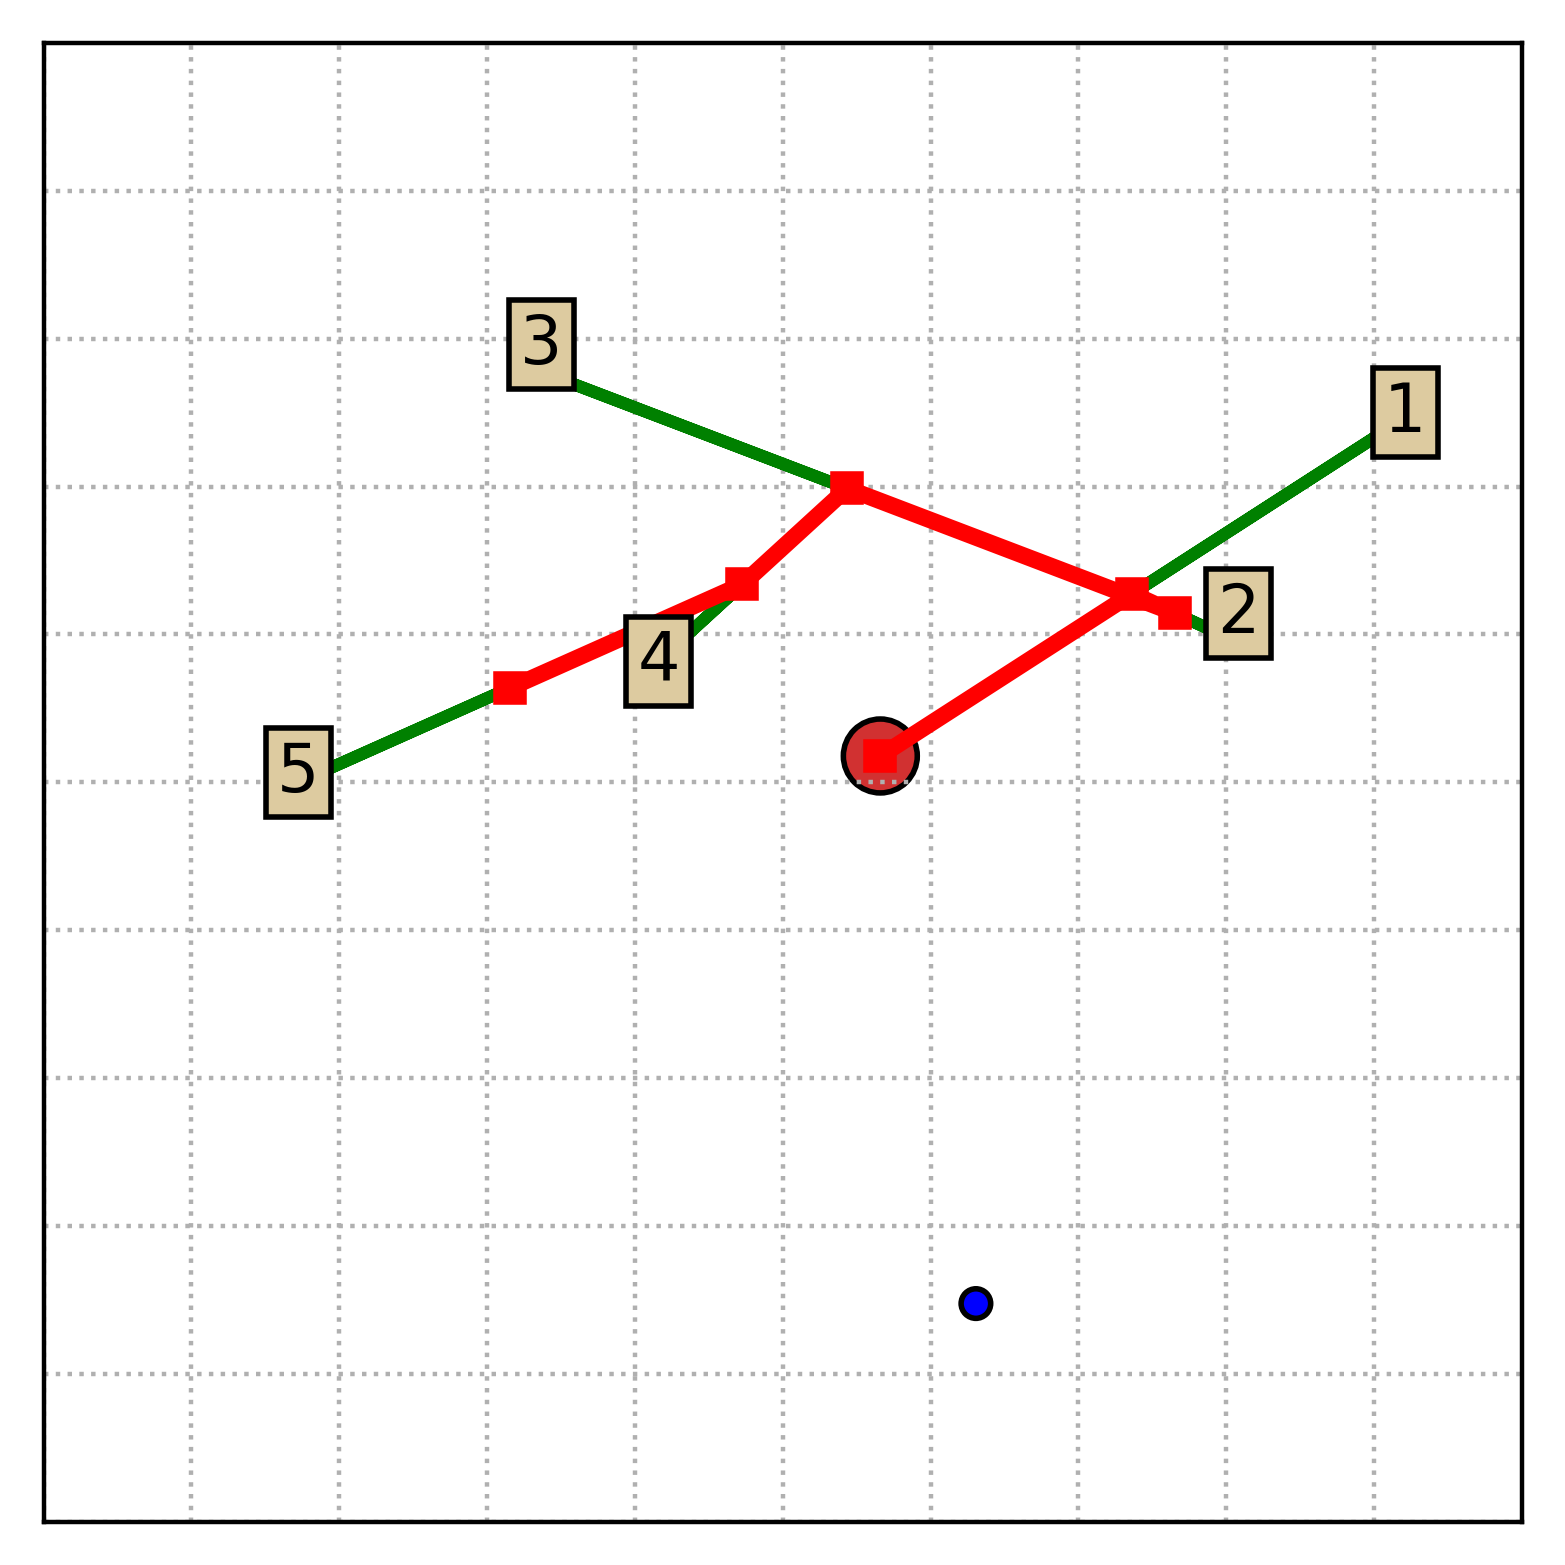
\includegraphics[width=8cm]{../webs/docs/algo-greedy-incremental-insertion---Day-2018-12-24_ClockTime-19:31:02/algo_state_00004.png}&
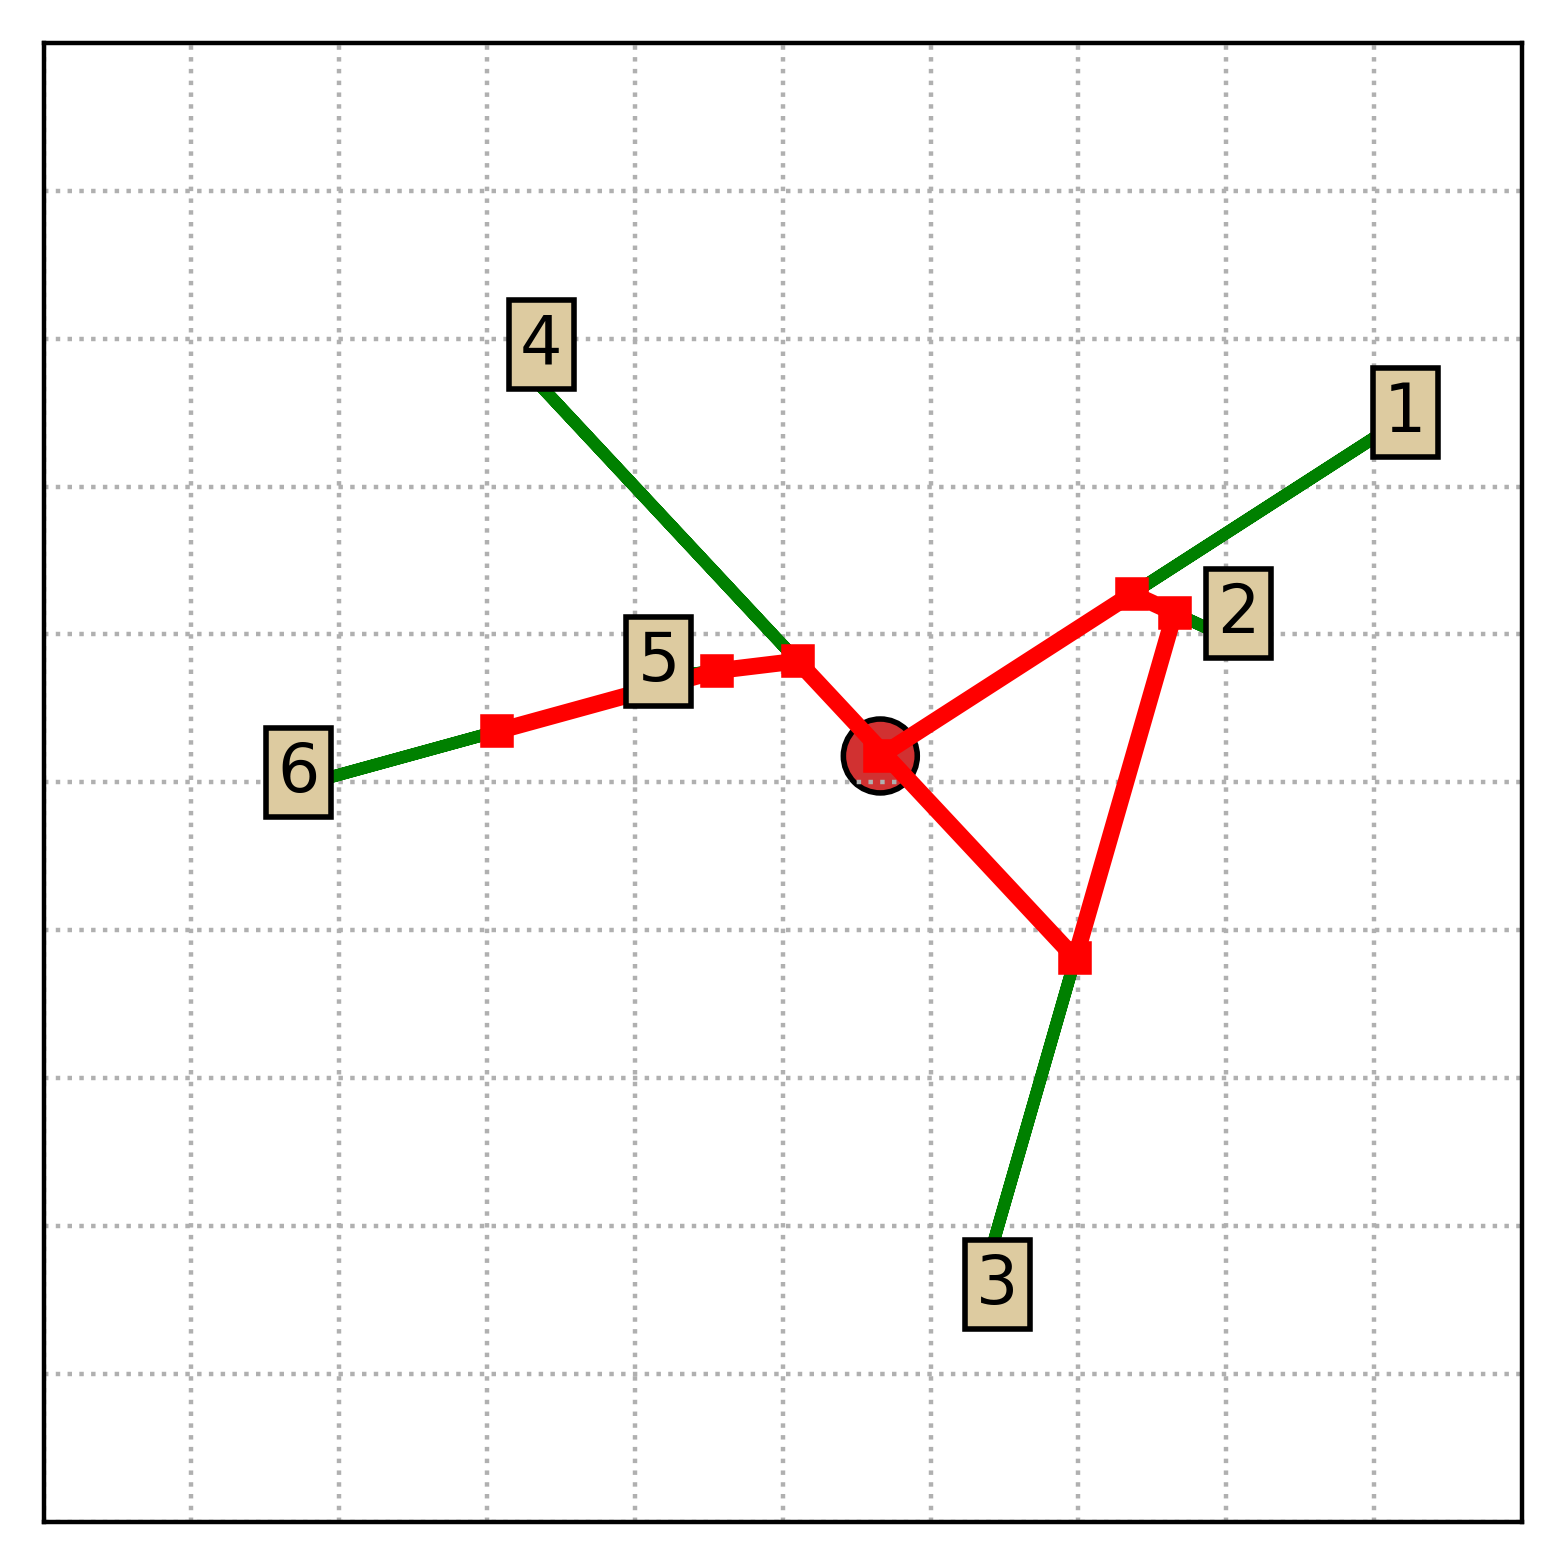
\includegraphics[width=8cm]{../webs/docs/algo-greedy-incremental-insertion---Day-2018-12-24_ClockTime-19:31:02/algo_state_00005.png}\\
\end{tabular}
\caption{Greedy incremental insertion for collinear horseflies. $\varphi=3.0$. Notice that 
the ordering of the visited sites keep changing based on where we decide to insert an 
unvisited site.}
\label{fig:greedy-incremental-example}
\end{figure}


\autoref{fig:greedy-incremental-example} depicts the incremental insertion process for 
the case of 4 sites and $\varphi=3$. Notice that the ordering of the visited sites keep 
changing based on where we decide to insert an unvisited site. 

The implementation of this algorithm for collinear-horseflies raises several interesting non-trivial 
data-structural questions in their own right: how to quickly find the site from $U$ to 
insert into $V$, and keep track the changing length of the horsefly tour. Note that inserting a site 
causes the length of the tour of the truck to change, for all the sites after $s$. 
 
\subsection*{Algorithmic Details}
\newchunk The implementation of the algorithm is ``parametrized'' over various strategies for insertion. 
i.e. we treat each insertion policy as a black-box argument to the function.
 
Efficient policies for detecting the exact or approximate point for cheapest insertion will be 
described in \autoref{subsec:insertion-policies}.  We also implement a ``naive'' policy as a way 
benchmark the quality and speed of implementation of future insertion policies. 

%{python-mode}%
\begin{flushleft} \small\label{scrap47}\raggedright\small
\NWtarget{nuweb38a}{} $\langle\,${\itshape Algorithms for classic horsefly}\nobreak\ {\footnotesize {38a}}$\,\rangle\equiv$
\vspace{-1ex}
\begin{list}{}{} \item
\mbox{}\verb@@\\
\mbox{}\verb@@\hbox{$\langle\,${\itshape Define auxiliary helper functions}\nobreak\ {\footnotesize \NWlink{nuweb44a}{44a}, \ldots\ }$\,\rangle$}\verb@@\\
\mbox{}\verb@@\hbox{$\langle\,${\itshape Define various insertion policy classes}\nobreak\ {\footnotesize \NWlink{nuweb45b}{45b}}$\,\rangle$}\verb@@\\
\mbox{}\verb@def algo_greedy_incremental_insertion(sites, inithorseposn, phi,@\\
\mbox{}\verb@                                      insertion_policy_name       = "naive",@\\
\mbox{}\verb@                                      write_algo_states_to_disk_p = False   ,@\\
\mbox{}\verb@                                      animate_schedule_p          = True   , @\\
\mbox{}\verb@                                      post_optimizer              = None):@\\
\mbox{}\verb@      @\hbox{$\langle\,${\itshape Set log, algo-state and input-output files config}\nobreak\ {\footnotesize \NWlink{nuweb38b}{38b}}$\,\rangle$}\verb@@\\
\mbox{}\verb@      @\hbox{$\langle\,${\itshape Set insertion policy class for current run}\nobreak\ {\footnotesize \NWlink{nuweb39a}{39a}}$\,\rangle$}\verb@@\\
\mbox{}\verb@@\\
\mbox{}\verb@      while insertion_policy.unvisited_sites_idxs: @\\
\mbox{}\verb@         @\hbox{$\langle\,${\itshape Use insertion policy to find the cheapest site to insert into current tour}\nobreak\ {\footnotesize \NWlink{nuweb39b}{39b}}$\,\rangle$}\verb@@\\
\mbox{}\verb@         @\hbox{$\langle\,${\itshape Write algorithms current state to file}\nobreak\ {\footnotesize \NWlink{nuweb40a}{40a}}$\,\rangle$}\verb@@\\
\mbox{}\verb@@\\
\mbox{}\verb@      @\hbox{$\langle\,${\itshape Write input and output to file}\nobreak\ {\footnotesize \NWlink{nuweb43a}{43a}}$\,\rangle$}\verb@@\\
\mbox{}\verb@      @\hbox{$\langle\,${\itshape Make an animation of the schedule, if \verb|animate_schedule_p == True|}\nobreak\ {\footnotesize \NWlink{nuweb43c}{43c}}$\,\rangle$}\verb@@\\
\mbox{}\verb@      #sys.exit()@\\
\mbox{}\verb@      @\hbox{$\langle\,${\itshape Make an animation of algorithm states, if \verb|write_algo_states_to_disk_p == True|}\nobreak\ {\footnotesize \NWlink{nuweb43b}{43b}}$\,\rangle$}\verb@@\\
\mbox{}\verb@      @\hbox{$\langle\,${\itshape Return horsefly tour, along with additional information}\nobreak\ {\footnotesize \NWlink{nuweb43d}{43d}}$\,\rangle$}\verb@@\\
\mbox{}\verb@@{\NWsep}
\end{list}
\vspace{-1.5ex}
\footnotesize
\begin{list}{}{\setlength{\itemsep}{-\parsep}\setlength{\itemindent}{-\leftmargin}}
\item \NWtxtMacroDefBy\ \NWlink{nuweb27}{27}\NWlink{nuweb28}{, 28}\NWlink{nuweb31a}{, 31a}\NWlink{nuweb32b}{, 32b}\NWlink{nuweb38a}{, 38a}\NWlink{nuweb51}{, 51}\NWlink{nuweb54}{, 54}\NWlink{nuweb56}{, 56}.
\item \NWtxtMacroRefIn\ \NWlink{nuweb20a}{20a}.
\item \NWtxtIdentsDefed\nobreak\  \verb@algo_greedy_incremental_insertion,@\nobreak\ \NWlink{nuweb22}{22}, \verb@write_algo_states_to_disk_p@\nobreak\ \NWlink{nuweb28}{28}\NWlink{nuweb40a}{, 40a}\NWlink{nuweb40b}{b}\NWlink{nuweb43b}{, 43b}.
\item{}
\end{list}
\vspace{4ex}
\end{flushleft}
%{/python-mode}%


\vspace{-0.8cm}\newchunk Note that for each run of the algorithm, we create a dedicated directory and 
use a corresponding log file  in that directory. It will typically containe detailed 
information on the progress of the algorithm and the steps executed. 

For algorithm analysis, and verification of correctness,on the other hand, we will 
typically  be interested in the states of the data-structures at the end of 
the while loop; each such state will be written out as a YAML file. Such files can 
be useful for animating the progress of the algorithm. 

Finally, just before returning the answer, we write the input and output 
to a separate YAML file. All in all, there are three ``types'' of output files
within each directory that corresponds to an algorithm's run: 
\underline{a log file}, \underline{algorithm states files}, and finally 
an \underline{input-output file}. 

%{python-mode}%
\begin{flushleft} \small\label{scrap48}\raggedright\small
\NWtarget{nuweb38b}{} $\langle\,${\itshape Set log, algo-state and input-output files config}\nobreak\ {\footnotesize {38b}}$\,\rangle\equiv$
\vspace{-1ex}
\begin{list}{}{} \item
\mbox{}\verb@  @\\
\mbox{}\verb@import sys, logging, datetime, os, errno@\\
\mbox{}\verb@@\\
\mbox{}\verb@algo_name     = 'algo-greedy-incremental-insertion'@\\
\mbox{}\verb@time_stamp    = datetime.datetime.now().strftime('Day-%Y-%m-%d_ClockTime-%H:%M:%S')@\\
\mbox{}\verb@dir_name      = algo_name + '---' + time_stamp@\\
\mbox{}\verb@log_file_name = dir_name + '/' + 'run.log'@\\
\mbox{}\verb@io_file_name  = 'input_and_output.yml'@\\
\mbox{}\verb@@\\
\mbox{}\verb@# Create directory for writing data-files and logs to for @\\
\mbox{}\verb@# current run of this algorithm@\\
\mbox{}\verb@try:@\\
\mbox{}\verb@    os.makedirs(dir_name)@\\
\mbox{}\verb@except OSError as e:@\\
\mbox{}\verb@    if e.errno != errno.EEXIST:@\\
\mbox{}\verb@        raise@\\
\mbox{}\verb@@\\
\mbox{}\verb@logging.basicConfig( filename = log_file_name,@\\
\mbox{}\verb@                     level    = logging.DEBUG,@\\
\mbox{}\verb@                     format   = '%(asctime)s: %(levelname)s: %(message)s',@\\
\mbox{}\verb@                     filemode = 'w' )@\\
\mbox{}\verb@#logger = logging.getLogger()@\\
\mbox{}\verb@info("Started running greedy_incremental_insertion for classic horsefly")@\\
\mbox{}\verb@@\\
\mbox{}\verb@algo_state_counter = 1 @\\
\mbox{}\verb@@{\NWsep}
\end{list}
\vspace{-1.5ex}
\footnotesize
\begin{list}{}{\setlength{\itemsep}{-\parsep}\setlength{\itemindent}{-\leftmargin}}
\item \NWtxtMacroRefIn\ \NWlink{nuweb38a}{38a}.
\item \NWtxtIdentsDefed\nobreak\  \verb@io_file_name,@\nobreak\ \NWlink{nuweb30b}{30b}\NWlink{nuweb43a}{, 43a}, \verb@logger@\nobreak\ \NWlink{nuweb21a}{21a}\NWlink{nuweb29a}{, 29a}.\item \NWtxtIdentsUsed\nobreak\  \verb@greedy@\nobreak\ \NWlink{nuweb30a}{30a}.
\item{}
\end{list}
\vspace{4ex}
\end{flushleft}
%{/python-mode}%

\vspace{-0.8cm}\newchunk This fragment merely sets the variable \verb|insertion_policy| to 
the appropriate function. This will later help us in studying the speed of 
the algorithm and quality of the solution for various insertion policies 
during the experimental analysis. 

%{python-mode}%
\begin{flushleft} \small\label{scrap49}\raggedright\small
\NWtarget{nuweb39a}{} $\langle\,${\itshape Set insertion policy class for current run}\nobreak\ {\footnotesize {39a}}$\,\rangle\equiv$
\vspace{-1ex}
\begin{list}{}{} \item
\mbox{}\verb@@\\
\mbox{}\verb@if insertion_policy_name == "naive":@\\
\mbox{}\verb@     insertion_policy = PolicyBestInsertionNaive(sites, inithorseposn, phi)@\\
\mbox{}\verb@else: @\\
\mbox{}\verb@     print insertion_policy_name@\\
\mbox{}\verb@     sys.exit("Unknown insertion policy: ")@\\
\mbox{}\verb@debug("Finished setting insertion policy: " + insertion_policy_name)@\\
\mbox{}\verb@@{\NWsep}
\end{list}
\vspace{-1.5ex}
\footnotesize
\begin{list}{}{\setlength{\itemsep}{-\parsep}\setlength{\itemindent}{-\leftmargin}}
\item \NWtxtMacroRefIn\ \NWlink{nuweb38a}{38a}.

\item{}
\end{list}
\vspace{4ex}
\end{flushleft}
%{/python-mode}%

\vspace{-0.8cm}\newchunk Note that while defining the body of the algorithm, we treat the insertion policy 
(whose name has already been passed as an string argument) as a kind of black-box, since all 
policy classes have the same interface. The detailed implementation for the various 
insertion policies are given later. 

%{python-mode}%
\begin{flushleft} \small\label{scrap50}\raggedright\small
\NWtarget{nuweb39b}{} $\langle\,${\itshape Use insertion policy to find the cheapest site to insert into current tour}\nobreak\ {\footnotesize {39b}}$\,\rangle\equiv$
\vspace{-1ex}
\begin{list}{}{} \item
\mbox{}\verb@insertion_policy.insert_another_unvisited_site()@\\
\mbox{}\verb@debug(Fore.GREEN + "Inserted another unvisited site" + Style.RESET_ALL)@\\
\mbox{}\verb@@{\NWsep}
\end{list}
\vspace{-1.5ex}
\footnotesize
\begin{list}{}{\setlength{\itemsep}{-\parsep}\setlength{\itemindent}{-\leftmargin}}
\item \NWtxtMacroRefIn\ \NWlink{nuweb38a}{38a}.

\item{}
\end{list}
\vspace{4ex}
\end{flushleft}
%{/python-mode}%

\vspace{-0.8cm}\newchunk When using Python 2.7 (as I am doing with this suite of programs), you should have the 
\texttt{pyyaml} module version 3.12 installed. Version 4.1 breaks for some weird reason; it can't seem to serialized
Numpy objects. See \url{https://github.com/kevin1024/vcrpy/issues/366} for a brief discussion on this topic. 

The version of \verb|pyyaml| on your machine can be checked by printing the value of \verb|yaml.__version__|. 
To install the correct version of pyyaml (if you get errors)  use

\begin{verbatim} 
              sudo pip uninstall pyyaml && sudo pip install pyyaml=3.12
\end{verbatim}

\newchunk We use the \verb|write_algo_states_to_disk_p| boolean argument to explicitly specify whether to write 
the current algorithm state along with its image to disk or not. This is because Matplotlib and PyYaml
is \underline{very} slow when writing image files to disk. Later on, I will probably switch to Asymptote 
for all my plotting, but for the moment I will stick to Matplotlib because I don't want to have to switch languages right now. 
 
And much of my plots will be of a reasonably high-quality for the purpose of presentations. This will naturally 
affect timing/benchmarking results. 

%{python-mode}%
\begin{flushleft} \small\label{scrap51}\raggedright\small
\NWtarget{nuweb40a}{} $\langle\,${\itshape Write algorithms current state to file}\nobreak\ {\footnotesize {40a}}$\,\rangle\equiv$
\vspace{-1ex}
\begin{list}{}{} \item
\mbox{}\verb@if write_algo_states_to_disk_p:@\\
\mbox{}\verb@     import yaml@\\
\mbox{}\verb@     algo_state_file_name = 'algo_state_'                    + \@\\
\mbox{}\verb@                       str(algo_state_counter).zfill(5) + \@\\
\mbox{}\verb@                       '.yml'@\\
\mbox{}\verb@@\\
\mbox{}\verb@     data = {'insertion_policy_name' : insertion_policy_name                       ,@\\
\mbox{}\verb@             'unvisited_sites'       : [insertion_policy.sites[u] \@\\
\mbox{}\verb@                                            for u in insertion_policy.unvisited_sites_idxs], @\\
\mbox{}\verb@             'visited_sites'         : insertion_policy.visited_sites                    , @\\
\mbox{}\verb@             'horse_tour'            : insertion_policy.horse_tour }@\\
\mbox{}\verb@@\\
\mbox{}\verb@     with open(dir_name + '/' + algo_state_file_name, 'w') as outfile:@\\
\mbox{}\verb@          yaml.dump( data   , \@\\
\mbox{}\verb@                     outfile, \@\\
\mbox{}\verb@                     default_flow_style = False)@\\
\mbox{}\verb@          @\hbox{$\langle\,${\itshape Render current algorithm state to image file}\nobreak\ {\footnotesize \NWlink{nuweb40b}{40b}}$\,\rangle$}\verb@@\\
\mbox{}\verb@@\\
\mbox{}\verb@     algo_state_counter = algo_state_counter + 1@\\
\mbox{}\verb@     debug("Dumped algorithm state to " + algo_state_file_name)@\\
\mbox{}\verb@@{\NWsep}
\end{list}
\vspace{-1.5ex}
\footnotesize
\begin{list}{}{\setlength{\itemsep}{-\parsep}\setlength{\itemindent}{-\leftmargin}}
\item \NWtxtMacroRefIn\ \NWlink{nuweb38a}{38a}.
\item \NWtxtIdentsUsed\nobreak\  \verb@write_algo_states_to_disk_p@\nobreak\ \NWlink{nuweb38a}{38a}.
\item{}
\end{list}
\vspace{4ex}
\end{flushleft}
%{/python-mode}%


\vspace{-0.4cm}

%{python-mode}%
\begin{flushleft} \small\label{scrap52}\raggedright\small
\NWtarget{nuweb40b}{} $\langle\,${\itshape Render current algorithm state to image file}\nobreak\ {\footnotesize {40b}}$\,\rangle\equiv$
\vspace{-1ex}
\begin{list}{}{} \item
\mbox{}\verb@import utils_algo@\\
\mbox{}\verb@if write_algo_states_to_disk_p:@\\
\mbox{}\verb@     @\hbox{$\langle\,${\itshape Set up plotting area and canvas, fig, ax, and other configs}\nobreak\ {\footnotesize \NWlink{nuweb40c}{40c}}$\,\rangle$}\verb@  @\\
\mbox{}\verb@     @\hbox{$\langle\,${\itshape Extract $x$ and $y$ coordinates of the points on the horse, fly tours, visited and unvisited sites}\nobreak\ {\footnotesize \NWlink{nuweb41a}{41a}}$\,\rangle$}\verb@  @\\
\mbox{}\verb@     @\hbox{$\langle\,${\itshape Mark initial position of horse and fly boldly on canvas}\nobreak\ {\footnotesize \NWlink{nuweb41b}{41b}}$\,\rangle$}\verb@  @\\
\mbox{}\verb@     @\hbox{$\langle\,${\itshape Place numbered markers on visited sites to mark the order of visitation explicitly}\nobreak\ {\footnotesize \NWlink{nuweb41d}{41d}}$\,\rangle$}\verb@@\\
\mbox{}\verb@     @\hbox{$\langle\,${\itshape Draw horse and fly-tours}\nobreak\ {\footnotesize \NWlink{nuweb41c}{41c}}$\,\rangle$}\verb@@\\
\mbox{}\verb@     @\hbox{$\langle\,${\itshape Draw unvisited sites as filled blue circles}\nobreak\ {\footnotesize \NWlink{nuweb42a}{42a}}$\,\rangle$}\verb@@\\
\mbox{}\verb@     @\hbox{$\langle\,${\itshape Give metainformation about current picture as headers and footers}\nobreak\ {\footnotesize \NWlink{nuweb42b}{42b}}$\,\rangle$}\verb@@\\
\mbox{}\verb@     @\hbox{$\langle\,${\itshape Write image file}\nobreak\ {\footnotesize \NWlink{nuweb42c}{42c}}$\,\rangle$}\verb@@\\
\mbox{}\verb@@{\NWsep}
\end{list}
\vspace{-1.5ex}
\footnotesize
\begin{list}{}{\setlength{\itemsep}{-\parsep}\setlength{\itemindent}{-\leftmargin}}
\item \NWtxtMacroRefIn\ \NWlink{nuweb40a}{40a}.
\item \NWtxtIdentsUsed\nobreak\  \verb@write_algo_states_to_disk_p@\nobreak\ \NWlink{nuweb38a}{38a}.
\item{}
\end{list}
\vspace{4ex}
\end{flushleft}
%{/python-mode}%

\vspace{-0.8cm}\newchunk 

%{python-mode}%
\begin{flushleft} \small\label{scrap53}\raggedright\small
\NWtarget{nuweb40c}{} $\langle\,${\itshape Set up plotting area and canvas, fig, ax, and other configs}\nobreak\ {\footnotesize {40c}}$\,\rangle\equiv$
\vspace{-1ex}
\begin{list}{}{} \item
\mbox{}\verb@from matplotlib import rc@\\
\mbox{}\verb@rc('font', **{'family': 'serif', \@\\
\mbox{}\verb@           'serif': ['Computer Modern']})@\\
\mbox{}\verb@rc('text', usetex=True)@\\
\mbox{}\verb@fig,ax = plt.subplots()@\\
\mbox{}\verb@ax.set_xlim([0,1])@\\
\mbox{}\verb@ax.set_ylim([0,1])@\\
\mbox{}\verb@ax.set_aspect(1.0)@\\
\mbox{}\verb@ax = fig.gca()@\\
\mbox{}\verb@ax.set_xticks(np.arange(0, 1, 0.1))     @\\
\mbox{}\verb@ax.set_yticks(np.arange(0, 1., 0.1))@\\
\mbox{}\verb@plt.grid(linestyle='dotted')@\\
\mbox{}\verb@ax.set_xticklabels([]) # to remove those numbers at the bottom@\\
\mbox{}\verb@ax.set_yticklabels([])@\\
\mbox{}\verb@@\\
\mbox{}\verb@ax.tick_params(@\\
\mbox{}\verb@    bottom=False,      # ticks along the bottom edge are off@\\
\mbox{}\verb@    left=False,        # ticks along the top edge are off@\\
\mbox{}\verb@    labelbottom=False) # labels along the bottom edge are off@\\
\mbox{}\verb@@{\NWsep}
\end{list}
\vspace{-1.5ex}
\footnotesize
\begin{list}{}{\setlength{\itemsep}{-\parsep}\setlength{\itemindent}{-\leftmargin}}
\item \NWtxtMacroRefIn\ \NWlink{nuweb40b}{40b}.

\item{}
\end{list}
\vspace{4ex}
\end{flushleft}
%{/python-mode}%

\vspace{-0.8cm}\newchunk Matplotlib typically plots points using x and y coordinates of the points in separate points. 

%{python-mode}%
\begin{flushleft} \small\label{scrap54}\raggedright\small
\NWtarget{nuweb41a}{} $\langle\,${\itshape Extract $x$ and $y$ coordinates of the points on the horse, fly tours, visited and unvisited sites}\nobreak\ {\footnotesize {41a}}$\,\rangle\equiv$
\vspace{-1ex}
\begin{list}{}{} \item
\mbox{}\verb@# Route for the horse@\\
\mbox{}\verb@xhs = [ data['horse_tour'][i][0] \@\\
\mbox{}\verb@          for i in range(len(data['horse_tour']))  ]    @\\
\mbox{}\verb@yhs = [ data['horse_tour'][i][1] \@\\
\mbox{}\verb@          for i in range(len(data['horse_tour']))  ]    @\\
\mbox{}\verb@@\\
\mbox{}\verb@# Route for the fly. The fly keeps alternating between the site and the horse@\\
\mbox{}\verb@xfs , yfs = [xhs[0]], [yhs[0]]@\\
\mbox{}\verb@for site, pt in zip (data['visited_sites'],@\\
\mbox{}\verb@                     data['horse_tour'][1:]):@\\
\mbox{}\verb@    xfs.extend([site[0], pt[0]])@\\
\mbox{}\verb@    yfs.extend([site[1], pt[1]])@\\
\mbox{}\verb@        @\\
\mbox{}\verb@xvisited = [ data['visited_sites'][i][0] \@\\
\mbox{}\verb@               for i in range(len(data['visited_sites']))  ]    @\\
\mbox{}\verb@yvisited = [ data['visited_sites'][i][1] \@\\
\mbox{}\verb@               for i in range(len(data['visited_sites']))  ]    @\\
\mbox{}\verb@    @\\
\mbox{}\verb@xunvisited = [ data['unvisited_sites'][i][0] \@\\
\mbox{}\verb@                 for i in range(len(data['unvisited_sites']))  ]    @\\
\mbox{}\verb@yunvisited = [ data['unvisited_sites'][i][1] @\\
\mbox{}\verb@                 for i in range(len(data['unvisited_sites'])) ]    @\\
\mbox{}\verb@debug("Extracted x and y coordinates for route of horse, fly, visited and unvisited sites")@\\
\mbox{}\verb@@{\NWsep}
\end{list}
\vspace{-1.5ex}
\footnotesize
\begin{list}{}{\setlength{\itemsep}{-\parsep}\setlength{\itemindent}{-\leftmargin}}
\item \NWtxtMacroRefIn\ \NWlink{nuweb40b}{40b}.

\item{}
\end{list}
\vspace{4ex}
\end{flushleft}
%{/python-mode}%

\vspace{-0.8cm}\newchunk 

%{python-mode}%
\begin{flushleft} \small\label{scrap55}\raggedright\small
\NWtarget{nuweb41b}{} $\langle\,${\itshape Mark initial position of horse and fly boldly on canvas}\nobreak\ {\footnotesize {41b}}$\,\rangle\equiv$
\vspace{-1ex}
\begin{list}{}{} \item
\mbox{}\verb@ax.add_patch( mpl.patches.Circle( inithorseposn, \@\\
\mbox{}\verb@                                  radius = 1/55.0,\@\\
\mbox{}\verb@                                  facecolor= '#D13131', #'red',\@\\
\mbox{}\verb@                                  edgecolor='black')  )@\\
\mbox{}\verb@debug("Marked the initial position of horse and fly on canvas")@\\
\mbox{}\verb@@{\NWsep}
\end{list}
\vspace{-1.5ex}
\footnotesize
\begin{list}{}{\setlength{\itemsep}{-\parsep}\setlength{\itemindent}{-\leftmargin}}
\item \NWtxtMacroRefIn\ \NWlink{nuweb40b}{40b}.

\item{}
\end{list}
\vspace{4ex}
\end{flushleft}
%{/python-mode}%

%{python-mode}%
\begin{flushleft} \small
\begin{minipage}{\linewidth}\label{scrap56}\raggedright\small
\NWtarget{nuweb41c}{} $\langle\,${\itshape Draw horse and fly-tours}\nobreak\ {\footnotesize {41c}}$\,\rangle\equiv$
\vspace{-1ex}
\begin{list}{}{} \item
\mbox{}\verb@ax.plot(xfs,yfs,'g-',linewidth=1.1)  @\\
\mbox{}\verb@ax.plot(xhs, yhs, color='r', \@\\
\mbox{}\verb@        marker='s', markersize=3, \@\\
\mbox{}\verb@        linewidth=1.6) @\\
\mbox{}\verb@debug("Plotted the horse and fly tours")@\\
\mbox{}\verb@@{\NWsep}
\end{list}
\vspace{-1.5ex}
\footnotesize
\begin{list}{}{\setlength{\itemsep}{-\parsep}\setlength{\itemindent}{-\leftmargin}}
\item \NWtxtMacroRefIn\ \NWlink{nuweb40b}{40b}.

\item{}
\end{list}
\end{minipage}\vspace{4ex}
\end{flushleft}
%{/python-mode}%

%{python-mode}%
\begin{flushleft} \small\label{scrap57}\raggedright\small
\NWtarget{nuweb41d}{} $\langle\,${\itshape Place numbered markers on visited sites to mark the order of visitation explicitly}\nobreak\ {\footnotesize {41d}}$\,\rangle\equiv$
\vspace{-1ex}
\begin{list}{}{} \item
\mbox{}\verb@for x,y,i in zip(xvisited, yvisited, range(len(xvisited))):@\\
\mbox{}\verb@     ax.text(x, y, str(i+1),  fontsize=8, \@\\
\mbox{}\verb@             bbox=dict(facecolor='#ddcba0', alpha=1.0, pad=2.0)) @\\
\mbox{}\verb@debug("Placed numbered markers on visited sites")@\\
\mbox{}\verb@@{\NWsep}
\end{list}
\vspace{-1.5ex}
\footnotesize
\begin{list}{}{\setlength{\itemsep}{-\parsep}\setlength{\itemindent}{-\leftmargin}}
\item \NWtxtMacroRefIn\ \NWlink{nuweb40b}{40b}.

\item{}
\end{list}
\vspace{4ex}
\end{flushleft}
%{/python-mode}%

%{python-mode}%
\begin{flushleft} \small\label{scrap58}\raggedright\small
\NWtarget{nuweb42a}{} $\langle\,${\itshape Draw unvisited sites as filled blue circles}\nobreak\ {\footnotesize {42a}}$\,\rangle\equiv$
\vspace{-1ex}
\begin{list}{}{} \item
\mbox{}\verb@for x, y in zip(xunvisited, yunvisited):@\\
\mbox{}\verb@     ax.add_patch( mpl.patches.Circle( (x,y),\@\\
\mbox{}\verb@                                    radius    = 1/100.0,\@\\
\mbox{}\verb@                                    facecolor = 'blue',\@\\
\mbox{}\verb@                                    edgecolor = 'black')  )@\\
\mbox{}\verb@debug("Drew univisted sites")@\\
\mbox{}\verb@@{\NWsep}
\end{list}
\vspace{-1.5ex}
\footnotesize
\begin{list}{}{\setlength{\itemsep}{-\parsep}\setlength{\itemindent}{-\leftmargin}}
\item \NWtxtMacroRefIn\ \NWlink{nuweb40b}{40b}.

\item{}
\end{list}
\vspace{4ex}
\end{flushleft}
%{/python-mode}%


\vspace{-0.8cm}\newchunk 

%{python-mode}%
\begin{flushleft} \small\label{scrap59}\raggedright\small
\NWtarget{nuweb42b}{} $\langle\,${\itshape Give metainformation about current picture as headers and footers}\nobreak\ {\footnotesize {42b}}$\,\rangle\equiv$
\vspace{-1ex}
\begin{list}{}{} \item
\mbox{}\verb@fontsize = 15@\\
\mbox{}\verb@ax.set_title( r'Number of sites visited so far: ' +\@\\
\mbox{}\verb@               str(len(data['visited_sites']))   +\@\\
\mbox{}\verb@               '/' + str(len(sites))           ,  \@\\
\mbox{}\verb@                    fontdict={'fontsize':fontsize})@\\
\mbox{}\verb@ax.set_xlabel(r'$\varphi=$'+str(phi), fontdict={'fontsize':fontsize})@\\
\mbox{}\verb@debug("Setting title, headers, footers, etc...")@\\
\mbox{}\verb@@{\NWsep}
\end{list}
\vspace{-1.5ex}
\footnotesize
\begin{list}{}{\setlength{\itemsep}{-\parsep}\setlength{\itemindent}{-\leftmargin}}
\item \NWtxtMacroRefIn\ \NWlink{nuweb40b}{40b}.

\item{}
\end{list}
\vspace{4ex}
\end{flushleft}
%{/python-mode}%

\vspace{-0.8cm}
Note that after writing image files, you should close the current figure. Otherwise
the collection of all the open figures starts hogging the RAM. Matplotlib throws a
a warning to this effect (if you don't close to the figures) after writing about 
20 figures:

\begin{CVerbatim}[fontsize=\small]
/usr/local/lib/python2.7/dist-packages/matplotlib/pyplot.py:528: RuntimeWarning: 
More than 20 figures have been opened. Figures created through the pyplot interface 
(`matplotlib.pyplot.figure`) are retained until explicitly closed and may consume 
too much memory. (To control this warning, see the rcParam `figure.max_open_warning`).
max_open_warning, RuntimeWarning)
\end{CVerbatim}

There is a  Stack Overflow answer (\url{https://stackoverflow.com/a/21884375/505306}) 
which advises to call \verb|plt.close()| after writing out a file that closes the 
\textit{current} figure to avoid the above warning. 
%{python-mode}%
\begin{flushleft} \small\label{scrap60}\raggedright\small
\NWtarget{nuweb42c}{} $\langle\,${\itshape Write image file}\nobreak\ {\footnotesize {42c}}$\,\rangle\equiv$
\vspace{-1ex}
\begin{list}{}{} \item
\mbox{}\verb@image_file_name = 'algo_state_'                    +\@\\
\mbox{}\verb@                  str(algo_state_counter).zfill(5) +\@\\
\mbox{}\verb@                     '.png'@\\
\mbox{}\verb@plt.savefig(dir_name + '/' + image_file_name,  \@\\
\mbox{}\verb@            bbox_inches='tight', dpi=250)@\\
\mbox{}\verb@print "Wrote " + image_file_name + " to disk"   @\\
\mbox{}\verb@plt.close() @\\
\mbox{}\verb@debug(Fore.BLUE+"Rendered algorithm state to image file"+Style.RESET_ALL)@\\
\mbox{}\verb@@{\NWsep}
\end{list}
\vspace{-1.5ex}
\footnotesize
\begin{list}{}{\setlength{\itemsep}{-\parsep}\setlength{\itemindent}{-\leftmargin}}
\item \NWtxtMacroRefIn\ \NWlink{nuweb40b}{40b}.

\item{}
\end{list}
\vspace{4ex}
\end{flushleft}
%{/python-mode}%


\vspace{-0.8cm}\newchunk The final answer is written to disk in the form of a YAML file. It lists the input sites 
in the order of visitation computed by the algorithm and gives the tour of the horse. 
Note that the number of points on the horse's tour is 1 more than the number of given sites. 
%{python-mode}%
\begin{flushleft} \small\label{scrap61}\raggedright\small
\NWtarget{nuweb43a}{} $\langle\,${\itshape Write input and output to file}\nobreak\ {\footnotesize {43a}}$\,\rangle\equiv$
\vspace{-1ex}
\begin{list}{}{} \item
\mbox{}\verb@# ASSERT: `inithorseposn` is included as first point of the tour@\\
\mbox{}\verb@assert(len(insertion_policy.horse_tour) == len(insertion_policy.visited_sites) + 1) @\\
\mbox{}\verb@@\\
\mbox{}\verb@# ASSERT: All sites have been visited. Simple sanity check @\\
\mbox{}\verb@assert(len(insertion_policy.sites)   == len(insertion_policy.visited_sites)) @\\
\mbox{}\verb@@\\
\mbox{}\verb@data = {'insertion_policy_name' : insertion_policy_name   ,@\\
\mbox{}\verb@        'visited_sites'  : insertion_policy.visited_sites , @\\
\mbox{}\verb@        'horse_tour'     : insertion_policy.horse_tour    , @\\
\mbox{}\verb@        'phi'            : insertion_policy.phi           , @\\
\mbox{}\verb@        'inithorseposn'  : insertion_policy.inithorseposn}@\\
\mbox{}\verb@@\\
\mbox{}\verb@import yaml@\\
\mbox{}\verb@with open(dir_name + '/' + io_file_name, 'w') as outfile:     yaml.dump( data, \@\\
\mbox{}\verb@                outfile, \@\\
\mbox{}\verb@                default_flow_style=False)@\\
\mbox{}\verb@debug("Dumped input and output to " + io_file_name)@\\
\mbox{}\verb@@{\NWsep}
\end{list}
\vspace{-1.5ex}
\footnotesize
\begin{list}{}{\setlength{\itemsep}{-\parsep}\setlength{\itemindent}{-\leftmargin}}
\item \NWtxtMacroRefIn\ \NWlink{nuweb38a}{38a}.
\item \NWtxtIdentsUsed\nobreak\  \verb@io_file_name,@\nobreak\ \NWlink{nuweb38b}{38b}.
\item{}
\end{list}
\vspace{4ex}
\end{flushleft}
%{/python-mode}%

\vspace{-0.8cm}\newchunk If algorithm states have been rendered to files in the run-folder, we stitch them together using \verb|ffmpeg|
and make an \verb|.avi| animation of the changing states of the algorithms. The \verb|.avi| file will be in the algorithm's
run folder. I used the  tutorial given on \url{https://en.wikibooks.org/wiki/FFMPEG_An_Intermediate_Guide/image_sequence}
for choosing the particular command-line options to \verb|ffmpeg| below. The options \texttt{-hide\_banner -loglevel panic} 
to quieten \verb|ffmpeg|'s output were suggested by  \url{https://superuser.com/a/1045060/102371} 


%{python-mode}%
\begin{flushleft} \small\label{scrap62}\raggedright\small
\NWtarget{nuweb43b}{} $\langle\,${\itshape Make an animation of algorithm states, if \verb|write_algo_states_to_disk_p == True|}\nobreak\ {\footnotesize {43b}}$\,\rangle\equiv$
\vspace{-1ex}
\begin{list}{}{} \item
\mbox{}\verb@if write_algo_states_to_disk_p:@\\
\mbox{}\verb@     import subprocess, os@\\
\mbox{}\verb@     os.chdir(dir_name)@\\
\mbox{}\verb@     subprocess.call( ['ffmpeg',  '-hide_banner', '-loglevel', 'verbose', \@\\
\mbox{}\verb@                       '-r', '1',  '-i', 'algo_state_%05d.png', \@\\
\mbox{}\verb@                       '-vcodec', 'mpeg4', '-r', '10' , \@\\
\mbox{}\verb@                       'algo_state_animation.avi']  )@\\
\mbox{}\verb@     os.chdir('../')@\\
\mbox{}\verb@@{\NWsep}
\end{list}
\vspace{-1.5ex}
\footnotesize
\begin{list}{}{\setlength{\itemsep}{-\parsep}\setlength{\itemindent}{-\leftmargin}}
\item \NWtxtMacroRefIn\ \NWlink{nuweb38a}{38a}.
\item \NWtxtIdentsUsed\nobreak\  \verb@write_algo_states_to_disk_p@\nobreak\ \NWlink{nuweb38a}{38a}.
\item{}
\end{list}
\vspace{4ex}
\end{flushleft}
%{/python-mode}%

\vspace{-0.8cm} \newchunk This chunks reads the information in the input-output file just written out as
a YAML file in the run-folder and then renders the process of the horse and fly moving around the plane 
delivering packages to sites. 
%{python-mode}%

\begin{flushleft} \small
\begin{minipage}{\linewidth}\label{scrap63}\raggedright\small
\NWtarget{nuweb43c}{} $\langle\,${\itshape Make an animation of the schedule, if \verb|animate_schedule_p == True|}\nobreak\ {\footnotesize {43c}}$\,\rangle\equiv$
\vspace{-1ex}
\begin{list}{}{} \item
\mbox{}\verb@   @\\
\mbox{}\verb@if animate_schedule_p : @\\
\mbox{}\verb@     animateSchedule(dir_name + '/' + io_file_name)@\\
\mbox{}\verb@@{\NWsep}
\end{list}
\vspace{-1.5ex}
\footnotesize
\begin{list}{}{\setlength{\itemsep}{-\parsep}\setlength{\itemindent}{-\leftmargin}}
\item \NWtxtMacroRefIn\ \NWlink{nuweb38a}{38a}.

\item{}
\end{list}
\end{minipage}\vspace{4ex}
\end{flushleft}
%{/python-mode}%

\vspace{-0.8cm}\newchunk 
%{python-mode}%

\begin{flushleft} \small\label{scrap64}\raggedright\small
\NWtarget{nuweb43d}{} $\langle\,${\itshape Return horsefly tour, along with additional information}\nobreak\ {\footnotesize {43d}}$\,\rangle\equiv$
\vspace{-1ex}
\begin{list}{}{} \item
\mbox{}\verb@debug("Returning answer")@\\
\mbox{}\verb@horse_waiting_times = np.zeros(len(sites)) # TODO write this to file later@\\
\mbox{}\verb@return {'tour_points'                : insertion_policy.horse_tour[1:],@\\
\mbox{}\verb@        'horse_waiting_times'        : horse_waiting_times, @\\
\mbox{}\verb@        'site_ordering'              : insertion_policy.visited_sites,@\\
\mbox{}\verb@        'tour_length_with_waiting_time_included': \@\\
\mbox{}\verb@                                       tour_length_with_waiting_time_included(\@\\
\mbox{}\verb@                                                    insertion_policy.horse_tour[1:], \@\\
\mbox{}\verb@                                                    horse_waiting_times, \@\\
\mbox{}\verb@                                                    inithorseposn)}@\\
\mbox{}\verb@@{\NWsep}
\end{list}
\vspace{-1.5ex}
\footnotesize
\begin{list}{}{\setlength{\itemsep}{-\parsep}\setlength{\itemindent}{-\leftmargin}}
\item \NWtxtMacroRefIn\ \NWlink{nuweb38a}{38a}.
\item \NWtxtIdentsUsed\nobreak\  \verb@tour_length_with_waiting_time_included@\nobreak\ \NWlink{nuweb57b}{57b}.
\item{}
\end{list}
\vspace{4ex}
\end{flushleft}
%{/python-mode}%

\vspace{-0.8cm}\newchunk We now define some of the functions that were referred to in the above chunks. 
Given the intial position of the truck and drone, and a list of sites, we need to compute 
the collinear horsefly tour length for the given ordering. This is the function that is 
used in every policy class while deciding which is the cheapest unvisited site to insert 
into the current ordering of visited sites. 

Note that the order in which sites are passed to this function matters. It 
assumes that you want to compute the collinear horseflies tour length for the 
sites \textit{in the given order.} 

For this, we use the formula for computing the rendezvous point when there is 
only a single site, given by the code-chunk below. 

%\begin{center}
%\missingfigure[figwidth=6cm]{Sigle site analytic}
%\end{center}
%{python-mode}%

\begin{flushleft} \small\label{scrap65}\raggedright\small
\NWtarget{nuweb44a}{} $\langle\,${\itshape Define auxiliary helper functions}\nobreak\ {\footnotesize {44a}}$\,\rangle\equiv$
\vspace{-1ex}
\begin{list}{}{} \item
\mbox{}\verb@def single_site_solution(site, horseposn, phi):@\\
\mbox{}\verb@     @\\
\mbox{}\verb@     h = np.asarray(horseposn)@\\
\mbox{}\verb@     s = np.asarray(site)@\\
\mbox{}\verb@     @\\
\mbox{}\verb@     hs_mag  = 1.0/np.linalg.norm(s-h) @\\
\mbox{}\verb@     hs_unit = 1.0/hs_mag * (s-h)@\\
\mbox{}\verb@     @\\
\mbox{}\verb@     r      = h +  2*hs_mag/(1+phi) * hs_unit # Rendezvous point@\\
\mbox{}\verb@     hr_mag = np.linalg.norm(r-h)@\\
\mbox{}\verb@@\\
\mbox{}\verb@     return (tuple(r), hr_mag) @\\
\mbox{}\verb@@{\NWsep}
\end{list}
\vspace{-1.5ex}
\footnotesize
\begin{list}{}{\setlength{\itemsep}{-\parsep}\setlength{\itemindent}{-\leftmargin}}
\item \NWtxtMacroDefBy\ \NWlink{nuweb44a}{44a}\NWlink{nuweb44b}{b}\NWlink{nuweb45a}{, 45a}.
\item \NWtxtMacroRefIn\ \NWlink{nuweb38a}{38a}.
\item \NWtxtIdentsDefed\nobreak\  \verb@single_site_solution@\nobreak\ \NWlink{nuweb44b}{44b}\NWlink{nuweb45a}{, 45a}\NWlink{nuweb50b}{, 50b}.
\item{}
\end{list}
\vspace{4ex}
\end{flushleft}
%{/python-mode}%

\vspace{-0.8cm}
With that the tour length functions for collinear horseflies can be implemented as 
an elementary instance of the fold pattern of functional programming. 
\footnote{Python has folds tucked away in some corner of its standard library. 
But I am not using it during the first hacky portion of this draft. Also Shane 
mentioned it has performance issues? Double-check this later!}

%{python-mode}%

\begin{flushleft} \small\label{scrap66}\raggedright\small
\NWtarget{nuweb44b}{} $\langle\,${\itshape Define auxiliary helper functions}\nobreak\ {\footnotesize {44b}}$\,\rangle\equiv$
\vspace{-1ex}
\begin{list}{}{} \item
\mbox{}\verb@def compute_collinear_horseflies_tour_length(sites, horseposn, phi):@\\
\mbox{}\verb@@\\
\mbox{}\verb@     if not sites: # No more sites, left to visit!@\\
\mbox{}\verb@          return 0@\\
\mbox{}\verb@     else:         # Some sites are still left on the itinerary@\\
\mbox{}\verb@@\\
\mbox{}\verb@          (rendezvous_pt, horse_travel_length) = single_site_solution(sites[0], horseposn, phi )@\\
\mbox{}\verb@          return horse_travel_length  + \@\\
\mbox{}\verb@                 compute_collinear_horseflies_tour_length( sites[1:], rendezvous_pt, phi )@\\
\mbox{}\verb@@{\NWsep}
\end{list}
\vspace{-1.5ex}
\footnotesize
\begin{list}{}{\setlength{\itemsep}{-\parsep}\setlength{\itemindent}{-\leftmargin}}
\item \NWtxtMacroDefBy\ \NWlink{nuweb44a}{44a}\NWlink{nuweb44b}{b}\NWlink{nuweb45a}{, 45a}.
\item \NWtxtMacroRefIn\ \NWlink{nuweb38a}{38a}.
\item \NWtxtIdentsDefed\nobreak\  \verb@compute_collinear_horseflies_tour_length@\nobreak\ \NWlink{nuweb46b}{46b}\NWlink{nuweb46d}{d}.\item \NWtxtIdentsUsed\nobreak\  \verb@single_site_solution@\nobreak\ \NWlink{nuweb44a}{44a}.
\item{}
\end{list}
\vspace{4ex}
\end{flushleft}
%{/python-mode}%

%{python-mode}%

\begin{flushleft} \small
\begin{minipage}{\linewidth}\label{scrap67}\raggedright\small
\NWtarget{nuweb45a}{} $\langle\,${\itshape Define auxiliary helper functions}\nobreak\ {\footnotesize {45a}}$\,\rangle\equiv$
\vspace{-1ex}
\begin{list}{}{} \item
\mbox{}\verb@def compute_collinear_horseflies_tour(sites, inithorseposn, phi):@\\
\mbox{}\verb@@\\
\mbox{}\verb@      horseposn         = inithorseposn@\\
\mbox{}\verb@      horse_tour_points = [inithorseposn]@\\
\mbox{}\verb@@\\
\mbox{}\verb@      for site in sites:@\\
\mbox{}\verb@          (rendezvous_pt, _) = single_site_solution(site, horseposn, phi )@\\
\mbox{}\verb@            @\\
\mbox{}\verb@          horse_tour_points.append(rendezvous_pt)@\\
\mbox{}\verb@          horseposn = rendezvous_pt@\\
\mbox{}\verb@@\\
\mbox{}\verb@      return horse_tour_points@\\
\mbox{}\verb@@{\NWsep}
\end{list}
\vspace{-1.5ex}
\footnotesize
\begin{list}{}{\setlength{\itemsep}{-\parsep}\setlength{\itemindent}{-\leftmargin}}
\item \NWtxtMacroDefBy\ \NWlink{nuweb44a}{44a}\NWlink{nuweb44b}{b}\NWlink{nuweb45a}{, 45a}.
\item \NWtxtMacroRefIn\ \NWlink{nuweb38a}{38a}.
\item \NWtxtIdentsDefed\nobreak\  \verb@compute_collinear_horseflies_tour@\nobreak\ \NWlink{nuweb47b}{47b}.\item \NWtxtIdentsUsed\nobreak\  \verb@single_site_solution@\nobreak\ \NWlink{nuweb44a}{44a}.
\item{}
\end{list}
\end{minipage}\vspace{4ex}
\end{flushleft}
%{/python-mode}%


\section{Insertion Policies} 
\label{subsec:insertion-policies}

We have finished implemented the entire algorithm, except 
for the implementation of the various insertion policy classes. 

The main job of an insertion policy class is to keep track 
of the  unvisited sites,  the order of the visited sites and the 
horsefly tour itself. Every time, the method \verb|.get_next_site(...)| is called, it 
chooses an appropriate (i.e. cheapest) unvisited site to insert 
into the current ordering, and update the set of visited and unvisited sites
and details of the horsefly tour.  

To do this quickly it will typically need auxiliary data-structures whose specifics 
will depend on the details of the policy chosen. 

\subsection{Naive Insertion} \quad First, a naive implementation
  of the cheapest insertion heuristic, that will be useful in future
  benchmarking of running times and solution quality for implementations 
  that are quicker but make more sophisticated uses of data-structures. 

  In this policy for each unvisited site we first find the 
  position in the current tour, which after insertion into that position
  amongst the visited sites yields the smallest increase in the 
  collinear-horseflies tour-length. 

  Then we pick the unvisited site which yields the overall smallest 
  increase in tour-length and insert it into its computed position
  from its previous paragraph. 
     
  Clearly this implementation and has at least quadratic running time. 
  Later on, we will be investigating algorithms and data-structures 
  for speeding up this operation. 

  The hope is to be able to find a dynamic data-structure to perform this 
  insertion in logarithmic time. Variations on tools such as the well-separated pair 
  decomposition might help achieve this goal. Jon Bentley
  used kd-trees to perform the insertion in his experimental TSP
  paper, but he wasn't dealing with the shifting tour structure
  as we have in horseflies. Also he did not deal with the question 
  of finding an approximate point for insertion. These 

\newchunk Since the interface for all policy classes will be the same, it is 
best, if have a base class for such classes. Since the details of 
the interface may change, I'll probably do this later. For now, 
I'll just keep all the policy classes completely separate while 
keeping the interface of the constructors and methods the same. 
I'll refactor things later. 

The plan in that case should be to make an abstract class that 
has an abstract method called \texttt{insert\_unvisited\_site}
and three data-fields made from the base-constructor named \texttt{sites}, \texttt{inithorseposn}
and \texttt{phi}. Classes which inherit this abstract base class, will 
add their own local data-members and methods for keeping track of 
data for insertion. 
%{python-mode}%

\begin{flushleft} \small\label{scrap68}\raggedright\small
\NWtarget{nuweb45b}{} $\langle\,${\itshape Define various insertion policy classes}\nobreak\ {\footnotesize {45b}}$\,\rangle\equiv$
\vspace{-1ex}
\begin{list}{}{} \item
\mbox{}\verb@class PolicyBestInsertionNaive:@\\
\mbox{}\verb@@\\
\mbox{}\verb@    def __init__(self, sites, inithorseposn, phi):@\\
\mbox{}\verb@@\\
\mbox{}\verb@         self.sites           = sites@\\
\mbox{}\verb@         self.inithorseposn   = inithorseposn@\\
\mbox{}\verb@         self.phi             = phi@\\
\mbox{}\verb@@\\
\mbox{}\verb@         self.visited_sites        = []                # The actual list of visited sites (not indices)@\\
\mbox{}\verb@         self.unvisited_sites_idxs = range(len(sites)) # This indexes into self.sites@\\
\mbox{}\verb@         self.horse_tour           = [self.inithorseposn]         @\\
\mbox{}\verb@@\\
\mbox{}\verb@    @\hbox{$\langle\,${\itshape Methods for \verb|PolicyBestInsertionNaive|}\nobreak\ {\footnotesize \NWlink{nuweb46a}{46a}}$\,\rangle$}\verb@@\\
\mbox{}\verb@@{\NWsep}
\end{list}
\vspace{-1.5ex}
\footnotesize
\begin{list}{}{\setlength{\itemsep}{-\parsep}\setlength{\itemindent}{-\leftmargin}}
\item \NWtxtMacroRefIn\ \NWlink{nuweb38a}{38a}.
\item \NWtxtIdentsDefed\nobreak\  \verb@self.horse_tour@\nobreak\ \NWlink{nuweb47b}{47b}, \verb@self.inithorseposn,@\nobreak\ \NWlink{nuweb25c}{25c}\NWlink{nuweb25d}{d}\NWlink{nuweb46b}{, 46b}\NWlink{nuweb46d}{d}\NWlink{nuweb47b}{, 47b}, \verb@self.sites,@\nobreak\ \NWlink{nuweb25c}{25c}\NWlink{nuweb25d}{d}, \verb@self.visited_sites,@\nobreak\ \NWlink{nuweb46b}{46b}\NWlink{nuweb47b}{, 47b}.
\item{}
\end{list}
\vspace{4ex}
\end{flushleft}
%{/python-mode}%

\vspace{-0.8cm}\newchunk 
%{python-mode}%
\begin{flushleft} \small\label{scrap69}\raggedright\small
\NWtarget{nuweb46a}{} $\langle\,${\itshape Methods for \verb|PolicyBestInsertionNaive|}\nobreak\ {\footnotesize {46a}}$\,\rangle\equiv$
\vspace{-1ex}
\begin{list}{}{} \item
\mbox{}\verb@def insert_another_unvisited_site(self):@\\
\mbox{}\verb@   @\hbox{$\langle\,${\itshape Compute the length of the tour that currently services the visited sites}\nobreak\ {\footnotesize \NWlink{nuweb46b}{46b}}$\,\rangle$}\verb@    @\\
\mbox{}\verb@   delta_increase_least_table = [] # tracking variable updated in for loop below@\\
\mbox{}\verb@@\\
\mbox{}\verb@   for u in self.unvisited_sites_idxs:@\\
\mbox{}\verb@      @\hbox{$\langle\,${\itshape Set up tracking variables local to this iteration}\nobreak\ {\footnotesize \NWlink{nuweb46c}{46c}}$\,\rangle$}\verb@@\\
\mbox{}\verb@      @\hbox{$\langle\,${\itshape If \texttt{self.sites[u]} is chosen for insertion, find best insertion position and update \texttt{delta\_increase\_least\_table}}\nobreak\ {\footnotesize \NWlink{nuweb46d}{46d}}$\,\rangle$}\verb@  @\\
\mbox{}\verb@                 @\\
\mbox{}\verb@   @\hbox{$\langle\,${\itshape Find the unvisited site which on insertion increases tour-length by the least amount}\nobreak\ {\footnotesize \NWlink{nuweb47a}{47a}}$\,\rangle$}\verb@     @\\
\mbox{}\verb@   @\hbox{$\langle\,${\itshape Update states for \texttt{PolicyBestInsertionNaive}}\nobreak\ {\footnotesize \NWlink{nuweb47b}{47b}}$\,\rangle$}\verb@ @\\
\mbox{}\verb@@{\NWsep}
\end{list}
\vspace{-1.5ex}
\footnotesize
\begin{list}{}{\setlength{\itemsep}{-\parsep}\setlength{\itemindent}{-\leftmargin}}
\item \NWtxtMacroRefIn\ \NWlink{nuweb45b}{45b}.
\item \NWtxtIdentsDefed\nobreak\  \verb@delta_increase_least_table@\nobreak\ \NWlink{nuweb46d}{46d}\NWlink{nuweb47a}{, 47a}.
\item{}
\end{list}
\vspace{4ex}
\end{flushleft}
%{/python-mode}%

\vspace{-0.8cm}\newchunk 

%{python-mode}%
\begin{flushleft} \small\label{scrap70}\raggedright\small
\NWtarget{nuweb46b}{} $\langle\,${\itshape Compute the length of the tour that currently services the visited sites}\nobreak\ {\footnotesize {46b}}$\,\rangle\equiv$
\vspace{-1ex}
\begin{list}{}{} \item
\mbox{}\verb@current_tour_length    = \@\\
\mbox{}\verb@         compute_collinear_horseflies_tour_length(\@\\
\mbox{}\verb@                    self.visited_sites,\@\\
\mbox{}\verb@                    self.inithorseposn,\@\\
\mbox{}\verb@                    self.phi) @\\
\mbox{}\verb@@{\NWsep}
\end{list}
\vspace{-1.5ex}
\footnotesize
\begin{list}{}{\setlength{\itemsep}{-\parsep}\setlength{\itemindent}{-\leftmargin}}
\item \NWtxtMacroRefIn\ \NWlink{nuweb46a}{46a}.
\item \NWtxtIdentsDefed\nobreak\  \verb@current_tour_length@\nobreak\ \NWlink{nuweb46d}{46d}.\item \NWtxtIdentsUsed\nobreak\  \verb@compute_collinear_horseflies_tour_length@\nobreak\ \NWlink{nuweb44b}{44b}, \verb@self.inithorseposn,@\nobreak\ \NWlink{nuweb45b}{45b}, \verb@self.visited_sites,@\nobreak\ \NWlink{nuweb45b}{45b}.
\item{}
\end{list}
\vspace{4ex}
\end{flushleft}
%{/python-mode}%

\vspace{-0.8cm}\newchunk 

%{python-mode}%
\begin{flushleft} \small\label{scrap71}\raggedright\small
\NWtarget{nuweb46c}{} $\langle\,${\itshape Set up tracking variables local to this iteration}\nobreak\ {\footnotesize {46c}}$\,\rangle\equiv$
\vspace{-1ex}
\begin{list}{}{} \item
\mbox{}\verb@ibest                = 0@\\
\mbox{}\verb@delta_increase_least = float("inf")@\\
\mbox{}\verb@@{\NWsep}
\end{list}
\vspace{-1.5ex}
\footnotesize
\begin{list}{}{\setlength{\itemsep}{-\parsep}\setlength{\itemindent}{-\leftmargin}}
\item \NWtxtMacroRefIn\ \NWlink{nuweb46a}{46a}.
\item \NWtxtIdentsDefed\nobreak\  \verb@delta_increase_least@\nobreak\ \NWlink{nuweb46d}{46d}, \verb@ibest,@\nobreak\ \NWlink{nuweb46d}{46d}.
\item{}
\end{list}
\vspace{4ex}
\end{flushleft}
%{/python-mode}%

\vspace{-0.8cm}\newchunk 

%{python-mode}%
\begin{flushleft} \small\label{scrap72}\raggedright\small
\NWtarget{nuweb46d}{} $\langle\,${\itshape If \texttt{self.sites[u]} is chosen for insertion, find best insertion position and update \texttt{delta\_increase\_least\_table}}\nobreak\ {\footnotesize {46d}}$\,\rangle\equiv$
\vspace{-1ex}
\begin{list}{}{} \item
\mbox{}\verb@for i in range(len(self.sites)):@\\
\mbox{}\verb@                    @\\
\mbox{}\verb@            visited_sites_test = self.visited_sites[:i] +\@\\
\mbox{}\verb@                                 [ self.sites[u] ]      +\@\\
\mbox{}\verb@                                 self.visited_sites[i:]@\\
\mbox{}\verb@                                      @\\
\mbox{}\verb@            tour_length_on_insertion = \@\\
\mbox{}\verb@                       compute_collinear_horseflies_tour_length(\@\\
\mbox{}\verb@                                  visited_sites_test,\@\\
\mbox{}\verb@                                  self.inithorseposn,\@\\
\mbox{}\verb@                                  self.phi) @\\
\mbox{}\verb@@\\
\mbox{}\verb@            delta_increase = tour_length_on_insertion - current_tour_length                         @\\
\mbox{}\verb@            assert(delta_increase >= 0)               @\\
\mbox{}\verb@@\\
\mbox{}\verb@            if delta_increase < delta_increase_least:@\\
\mbox{}\verb@                  delta_increase_least = delta_increase@\\
\mbox{}\verb@                  ibest                = i                                              @\\
\mbox{}\verb@                      @\\
\mbox{}\verb@delta_increase_least_table.append({'unvisited_site_idx'      : u    , \@\\
\mbox{}\verb@                                   'best_insertion_position' : ibest, \@\\
\mbox{}\verb@                                   'delta_increase'          : delta_increase_least})@\\
\mbox{}\verb@@{\NWsep}
\end{list}
\vspace{-1.5ex}
\footnotesize
\begin{list}{}{\setlength{\itemsep}{-\parsep}\setlength{\itemindent}{-\leftmargin}}
\item \NWtxtMacroRefIn\ \NWlink{nuweb46a}{46a}.
\item \NWtxtIdentsUsed\nobreak\  \verb@compute_collinear_horseflies_tour_length@\nobreak\ \NWlink{nuweb44b}{44b}, \verb@current_tour_length@\nobreak\ \NWlink{nuweb46b}{46b}, \verb@delta_increase_least@\nobreak\ \NWlink{nuweb46c}{46c}, \verb@delta_increase_least_table@\nobreak\ \NWlink{nuweb46a}{46a}, \verb@ibest,@\nobreak\ \NWlink{nuweb46c}{46c}, \verb@self.inithorseposn,@\nobreak\ \NWlink{nuweb45b}{45b}.
\item{}
\end{list}
\vspace{4ex}
\end{flushleft}
%{/python-mode}%


\vspace{-0.8cm}\newchunk 

%{python-mode}%
\begin{flushleft} \small\label{scrap73}\raggedright\small
\NWtarget{nuweb47a}{} $\langle\,${\itshape Find the unvisited site which on insertion increases tour-length by the least amount}\nobreak\ {\footnotesize {47a}}$\,\rangle\equiv$
\vspace{-1ex}
\begin{list}{}{} \item
\mbox{}\verb@best_table_entry = min(delta_increase_least_table, \@\\
\mbox{}\verb@                         key = lambda x: x['delta_increase'])@\\
\mbox{}\verb@         @\\
\mbox{}\verb@unvisited_site_idx_for_insertion = best_table_entry['unvisited_site_idx']@\\
\mbox{}\verb@insertion_position               = best_table_entry['best_insertion_position']@\\
\mbox{}\verb@delta_increase                   = best_table_entry['delta_increase']@\\
\mbox{}\verb@@{\NWsep}
\end{list}
\vspace{-1.5ex}
\footnotesize
\begin{list}{}{\setlength{\itemsep}{-\parsep}\setlength{\itemindent}{-\leftmargin}}
\item \NWtxtMacroRefIn\ \NWlink{nuweb46a}{46a}.
\item \NWtxtIdentsUsed\nobreak\  \verb@delta_increase_least_table@\nobreak\ \NWlink{nuweb46a}{46a}.
\item{}
\end{list}
\vspace{4ex}
\end{flushleft}
%{/python-mode}%


\vspace{-0.8cm}\newchunk 

%{python-mode}%
\begin{flushleft} \small\label{scrap74}\raggedright\small
\NWtarget{nuweb47b}{} $\langle\,${\itshape Update states for \texttt{PolicyBestInsertionNaive}}\nobreak\ {\footnotesize {47b}}$\,\rangle\equiv$
\vspace{-1ex}
\begin{list}{}{} \item
\mbox{}\verb@# Update visited and univisted sites info@\\
\mbox{}\verb@self.visited_sites = self.visited_sites[:insertion_position]      +\@\\
\mbox{}\verb@                     [self.sites[unvisited_site_idx_for_insertion]] +\@\\
\mbox{}\verb@                     self.visited_sites[insertion_position:]@\\
\mbox{}\verb@  @\\
\mbox{}\verb@self.unvisited_sites_idxs = filter( lambda elt: elt != unvisited_site_idx_for_insertion, \@\\
\mbox{}\verb@                                    self.unvisited_sites_idxs ) @\\
\mbox{}\verb@@\\
\mbox{}\verb@# Update the tour of the horse@\\
\mbox{}\verb@self.horse_tour = compute_collinear_horseflies_tour(\@\\
\mbox{}\verb@                           self.visited_sites,         \@\\
\mbox{}\verb@                           self.inithorseposn, \@\\
\mbox{}\verb@                           self.phi) @\\
\mbox{}\verb@@{\NWsep}
\end{list}
\vspace{-1.5ex}
\footnotesize
\begin{list}{}{\setlength{\itemsep}{-\parsep}\setlength{\itemindent}{-\leftmargin}}
\item \NWtxtMacroRefIn\ \NWlink{nuweb46a}{46a}.
\item \NWtxtIdentsUsed\nobreak\  \verb@compute_collinear_horseflies_tour@\nobreak\ \NWlink{nuweb45a}{45a}, \verb@self.horse_tour@\nobreak\ \NWlink{nuweb45b}{45b}, \verb@self.inithorseposn,@\nobreak\ \NWlink{nuweb45b}{45b}, \verb@self.visited_sites,@\nobreak\ \NWlink{nuweb45b}{45b}.
\item{}
\end{list}
\vspace{4ex}
\end{flushleft}
%{/python-mode}%
\newpage
\section{Lower Bound: The $\varphi$-Prim-MST}  

\subsection*{Overview}\hspace{0.1cm}
To compare the experimental performance of algorithms for NP-hard optimization 
problems wrt solution quality, it helps to have a cheaply computable lower bound 
that acts as a proxy for OPT. In the case of the TSP, a lower bound is the weight 
of the minimum spanning tree on the set of input sites.

To compute the MST on a set of points, on typically uses greedy algorithms such as 
those by Prim, Kruskal or Boruvka. To get a lower-bound for Horsefly, we define a 
network that we call the $\varphi$-Prim-MST by a simple generalization of Prim. 
Currently, we don't have a natural interpretation of this structure means in 
terms of the sites. This is something we need to add to our TODO list. 

\begin{center}
\missingfigure[figwidth=6cm]{Testing a long text string}
\end{center}

This is clearly a lower-bound on the weight of $OPT$ for Collinear Horsefly. However, 
I believe that the stronger statement is also true

\begin{fconj}
The weight of the $\varphi$-MST is a lower-bound on the length of the 
horse's tour in $OPT$ for the classic horsefly problem. 
\end{fconj}

The proof of this conjecture seems to be non-trivial off-hand. I'll put a hold on 
all my attempts so far to prove this, since I want the experiments to guide 
my intuition here. 

It is possible that there could be other lower bounds based on generalizing 
the steps in Kruskal's and Boruvka's algorithms. Based on the experimental 
success of the $\varphi$-MST's, I will think of the appropriate generalizations 
for them later. 

One particular experiment that I would be interested would be how bad is to check
the crossing structure of the edges. In the MST edges never cross. What is the 
structure of the crossing in $\varphi$-MSTs? That might help me in designing a local
search operation for the Horsefly problem. 

Also note, that the construction of this $\varphi$-Prim MST can be generalized to 
two or more flies (single horse) we buld two separate trees; with two or more drones
since we are interested in minimizing the makespan, probably we greedily them so that
the trees are well-balanced.....?????? dunno doesn't strike as clean now that I 
think of it. It certainly isn't as clean as my node-splitting horsefly framework. 
Hopefully, I can prove some sort of theorems on those later? 

\begin{note}
As I type this, a separate question strikes me to be of independent interest: 
\textit{Given a point-cloud in the plane, preprocess the points such that for a 
query $\varphi$ we can compute the $\varphi$-MST in linear time}. Perhaps the MST, 
itself could be useful for this augmented with some data-structures for performing 
ray-shooting in an arrangement of segments. One can use such a data-structure, for 
making a quick animation of the evolution of the $\varphi$-MST as we keep 
changing the $\varphi$-parameter, as one often does while playing with Mathematica's 
\texttt{Manipulate} function. Can we motivate this by saying $\varphi$ might be 
uncertain? I don't know, people would only find this interesting if the particular 
data-structure helps in the computation of horsefly like tours. 
\end{note}

\subsection*{Computing the $\varphi$-Prim-MST }

\newchunk For the purposes of this section we define the notion of a rendezvous 
point for an edge. Given a directed segment $\overrightarrow{XY}$ and a speed 
ratio $\varphi$, assume a horse and a fly are positioned at $X$ and there is a 
site that needs to be serviced at $Y$. The rendezvous point
of $\overrightarrow{XY}$ is that point along $R$ at which the horse and fly meet 
up at the earliest after the fly leaves $X$. Explicit formulae for computing this 
point have already been implemented in \verb|single_site_solution|, in one of the 
previous sections. 

\newchunk Prim's algorithm for computing MSTs is essentially a greedy incremental 
insertion process. The same structure is visible in the code fragment below. The only
essential change from Prim's original algorithm is that we ``grow'' the tree only from 
the rendezvous points computed while inserting a new edge into the existing partial 
tree on the set of sites. This process is animated in 
\autoref{fig:animating-growth-of-phi-prim-mst}

I have will be using the \verb|NetworkX| library (\url{https://networkx.github.io/}) for 
storing and manipulating graphs. For performing efficient nearest-neighbor searches for 
each rendezvous point in the partially constructed MST, I will use the \verb|scikit-learn| 
library (\url{https://scikit-learn.org/stable/modules/neighbors.html}). When porting 
my codes to C\texttt{++}, I will probably have to switch over to the Boost Graph library and 
David Mount's ANN for the same purposes(both these libraries have been optmized for speed). 

In the \verb|while| loop below, \verb|node_site_info| stores a tuple for each node in the tree 
consisting of
\begin{enumerate}
\item a node-id (this corresponds to a rendezvous point in the tree)
\item the index of the closest site in the array sites for the node (the site)
\item distance of the node to the site with the above index.
\end{enumerate}

%{python-mode}%
\begin{flushleft} \small\label{scrap75}\raggedright\small
\NWtarget{nuweb49a}{} $\langle\,${\itshape Lower bounds for classic horsefly}\nobreak\ {\footnotesize {49a}}$\,\rangle\equiv$
\vspace{-1ex}
\begin{list}{}{} \item
\mbox{}\verb@def compute_phi_prim_mst(sites, inithorseposn,phi):@\\
\mbox{}\verb@@\\
\mbox{}\verb@     import networkx as nx@\\
\mbox{}\verb@     from sklearn.neighbors import NearestNeighbors@\\
\mbox{}\verb@     @\\
\mbox{}\verb@     @\hbox{$\langle\,${\itshape Create singleton graph, with node at \verb|inithorseposn|}\nobreak\ {\footnotesize \NWlink{nuweb49b}{49b}}$\,\rangle$}\verb@@\\
\mbox{}\verb@@\\
\mbox{}\verb@     unmarked_sites_idxs = range(len(sites))@\\
\mbox{}\verb@     while unmarked_sites_idxs:@\\
\mbox{}\verb@          node_site_info = []@\\
\mbox{}\verb@          @\\
\mbox{}\verb@          @\hbox{$\langle\,${\itshape For each node, find the closest site}\nobreak\ {\footnotesize \NWlink{nuweb50a}{50a}}$\,\rangle$}\verb@    @\\
\mbox{}\verb@          @\hbox{$\langle\,${\itshape Find the node with the closest site, and generate the next node and edge for the $\varphi$-MST}\nobreak\ {\footnotesize \NWlink{nuweb50b}{50b}}$\,\rangle$}\verb@@\\
\mbox{}\verb@          @\\
\mbox{}\verb@          # Marking means removing from unmarked list :-D@\\
\mbox{}\verb@          unmarked_sites_idxs.remove(next_site_to_mark_idx)@\\
\mbox{}\verb@          @\\
\mbox{}\verb@     utils_algo.print_list(G.nodes.data())@\\
\mbox{}\verb@     utils_algo.print_list(G.edges.data())@\\
\mbox{}\verb@     return G@\\
\mbox{}\verb@@{\NWsep}
\end{list}
\vspace{-1.5ex}
\footnotesize
\begin{list}{}{\setlength{\itemsep}{-\parsep}\setlength{\itemindent}{-\leftmargin}}
\item \NWtxtMacroRefIn\ \NWlink{nuweb20a}{20a}.
\item \NWtxtIdentsDefed\nobreak\  \verb@compute_phi_prim_mst,@\nobreak\ \NWtxtIdentsNotUsed, \verb@unmarked_sites_idxs@\nobreak\ \NWlink{nuweb50a}{50a}.
\item{}
\end{list}
\vspace{4ex}
\end{flushleft}
%{/python-mode}%


\vspace{-0.8cm} \newchunk Every node in the tree stores its own id as an integer along with 
its X-Y coordinates and the X-Y coordinates of the sites that it will be joined to with a 
straight-line segment. At the beginning the single node of the tree at the initial position
of the horse and fly has not been joined to any sites, and hence is empty. 

%{python-mode}%
\begin{flushleft} \small
\begin{minipage}{\linewidth}\label{scrap76}\raggedright\small
\NWtarget{nuweb49b}{} $\langle\,${\itshape Create singleton graph, with node at \verb|inithorseposn|}\nobreak\ {\footnotesize {49b}}$\,\rangle\equiv$
\vspace{-1ex}
\begin{list}{}{} \item
\mbox{}\verb@G = nx.Graph()@\\
\mbox{}\verb@G.add_node(0, mycoordinates=inithorseposn, joined_site_coords=[])@\\
\mbox{}\verb@@{\NWsep}
\end{list}
\vspace{-1.5ex}
\footnotesize
\begin{list}{}{\setlength{\itemsep}{-\parsep}\setlength{\itemindent}{-\leftmargin}}
\item \NWtxtMacroRefIn\ \NWlink{nuweb49a}{49a}.

\item{}
\end{list}
\end{minipage}\vspace{4ex}
\end{flushleft}
%{/python-mode}%



\vspace{-0.8cm} \newchunk
%{python-mode}%
\begin{flushleft} \small
\begin{minipage}{\linewidth}\label{scrap77}\raggedright\small
\NWtarget{nuweb50a}{} $\langle\,${\itshape For each node, find the closest site}\nobreak\ {\footnotesize {50a}}$\,\rangle\equiv$
\vspace{-1ex}
\begin{list}{}{} \item
\mbox{}\verb@   @\\
\mbox{}\verb@for nodeid, nodeval in G.nodes.data():@\\
\mbox{}\verb@    current_node_coordinates = np.asarray(nodeval['mycoordinates'])@\\
\mbox{}\verb@    distances_of_current_node_to_sites = []@\\
\mbox{}\verb@               @\\
\mbox{}\verb@    # The following loop finds the nearest unmarked site. So far, I am @\\
\mbox{}\verb@    # using brute force for this, later, I will use sklearn.neighbors.@\\
\mbox{}\verb@    for j in unmarked_sites_idxs:@\\
\mbox{}\verb@        site_coordinates = np.asarray(sites[j])@\\
\mbox{}\verb@        dist             =  np.linalg.norm( site_coordinates - current_node_coordinates )@\\
\mbox{}\verb@                    @\\
\mbox{}\verb@        distances_of_current_node_to_sites.append( (j, dist) )@\\
\mbox{}\verb@@\\
\mbox{}\verb@        nearest_site_idx, distance_of_current_node_to_nearest_site = \@\\
\mbox{}\verb@                        min(distances_of_current_node_to_sites, key=lambda (_, d): d)@\\
\mbox{}\verb@@\\
\mbox{}\verb@        node_site_info.append((nodeid, \@\\
\mbox{}\verb@                                  nearest_site_idx, \@\\
\mbox{}\verb@                                  distance_of_current_node_to_nearest_site))@\\
\mbox{}\verb@@{\NWsep}
\end{list}
\vspace{-1.5ex}
\footnotesize
\begin{list}{}{\setlength{\itemsep}{-\parsep}\setlength{\itemindent}{-\leftmargin}}
\item \NWtxtMacroRefIn\ \NWlink{nuweb49a}{49a}.
\item \NWtxtIdentsUsed\nobreak\  \verb@unmarked_sites_idxs@\nobreak\ \NWlink{nuweb49a}{49a}.
\item{}
\end{list}
\end{minipage}\vspace{4ex}
\end{flushleft}
%{/python-mode}%

\needspace{3cm}
\vspace{-0.8cm} \newchunk
%{python-mode}%
\begin{flushleft} \small
\begin{minipage}{\linewidth}\label{scrap78}\raggedright\small
\NWtarget{nuweb50b}{} $\langle\,${\itshape Find the node with the closest site, and generate the next node and edge for the $\varphi$-MST}\nobreak\ {\footnotesize {50b}}$\,\rangle\equiv$
\vspace{-1ex}
\begin{list}{}{} \item
\mbox{}\verb@@\\
\mbox{}\verb@opt_node_idx,          \@\\
\mbox{}\verb@next_site_to_mark_idx, \@\\
\mbox{}\verb@distance_to_next_site_to_mark = min(node_site_info, key=lambda (h,k,d) : d)@\\
\mbox{}\verb@@\\
\mbox{}\verb@tmp = sites[next_site_to_mark_idx]@\\
\mbox{}\verb@G.nodes[opt_node_idx]['joined_site_coords'].append(  tmp   ) @\\
\mbox{}\verb@(r, h) = single_site_solution(tmp, G.nodes[opt_node_idx]['mycoordinates'], phi) @\\
\mbox{}\verb@          @\\
\mbox{}\verb@# Remember! indexing of nodes started at 0, thats why you set@\\
\mbox{}\verb@# numnodes to the index of the newly inserted node. @\\
\mbox{}\verb@newnodeid = len(list(G.nodes))@\\
\mbox{}\verb@@\\
\mbox{}\verb@# joined_site_coords will be updated in the future iterations of while :@\\
\mbox{}\verb@G.add_node(newnodeid, mycoordinates=r, joined_site_coords=[]) @\\
\mbox{}\verb@  @\\
\mbox{}\verb@# insert the edge weight, will be useful later when @\\
\mbox{}\verb@# computing sum total of all the edges.@\\
\mbox{}\verb@G.add_edge(opt_node_idx, newnodeid, weight=h ) @\\
\mbox{}\verb@@{\NWsep}
\end{list}
\vspace{-1.5ex}
\footnotesize
\begin{list}{}{\setlength{\itemsep}{-\parsep}\setlength{\itemindent}{-\leftmargin}}
\item \NWtxtMacroRefIn\ \NWlink{nuweb49a}{49a}.
\item \NWtxtIdentsUsed\nobreak\  \verb@single_site_solution@\nobreak\ \NWlink{nuweb44a}{44a}.
\item{}
\end{list}
\end{minipage}\vspace{4ex}
\end{flushleft}
%{/python-mode}%
\section{\framebox{Algorithm}: Doubling the $\varphi$-MST}  

\subsection{Algorithmic Overview}
\subsection{Algorithmic Details}
\section{\framebox{Algorithm}: Bottom-Up Split}  

\subsection{Algorithmic Overview}
\subsection{Algorithmic Details}\section{\framebox{Algorithm}: Local Search---Swap}  
\subsection{Algorithmic Overview}
\subsection{Algorithmic Details}
\section{\framebox{Algorithm}: K2 Means}  

\subsection{Algorithmic Overview}
\subsection{Algorithmic Details}
\newchunk
%{python-mode}%
\begin{flushleft} \small\label{scrap79}\raggedright\small
\NWtarget{nuweb51}{} $\langle\,${\itshape Algorithms for classic horsefly}\nobreak\ {\footnotesize {51}}$\,\rangle\equiv$
\vspace{-1ex}
\begin{list}{}{} \item
\mbox{}\verb@   @\\
\mbox{}\verb@def algo_kmeans(sites, inithorseposn, phi, k, post_optimizer):@\\
\mbox{}\verb@     """@\\
\mbox{}\verb@     type Point   (Double, Double)@\\
\mbox{}\verb@     type Site    Point@\\
\mbox{}\verb@     type Cluster (Point, [Site])@\\
\mbox{}\verb@     type Tour    {'site_ordering':[Site], @\\
\mbox{}\verb@                   'tour_points'  :[Point]}@\\
\mbox{}\verb@     algo_kmeans :: [Site] -> Point -> Double -> Int@\\
\mbox{}\verb@     """@\\
\mbox{}\verb@     def get_clusters(site_list):@\\
\mbox{}\verb@           """ @\\
\mbox{}\verb@           get_clusters :: [Site] -> [Cluster]@\\
\mbox{}\verb@           For the given list of sites, perform k-means clustering@\\
\mbox{}\verb@           and return the list of k-centers, along with a list of sites@\\
\mbox{}\verb@           assigned to each center. @\\
\mbox{}\verb@           """@\\
\mbox{}\verb@           X      = np.array(site_list)@\\
\mbox{}\verb@           kmeans = KMeans(n_clusters=k, random_state=0).fit(X)@\\
\mbox{}\verb@@\\
\mbox{}\verb@           accum = [ (center, [])  for center in kmeans.cluster_centers_ ]@\\
\mbox{}\verb@           for label, site in zip(kmeans.labels_, site_list):@\\
\mbox{}\verb@                 accum [label][1].append(site)@\\
\mbox{}\verb@@\\
\mbox{}\verb@           return accum @\\
\mbox{}\verb@@\\
\mbox{}\verb@     def extract_cluster_sites_for_each_cluster(clusters):@\\
\mbox{}\verb@         """@\\
\mbox{}\verb@         extract_cluster_sites_for_each_cluster :: [Cluster] -> [[Site]]@\\
\mbox{}\verb@         """@\\
\mbox{}\verb@         return [ cluster_sites for (_, cluster_sites) in clusters  ]@\\
\mbox{}\verb@@\\
\mbox{}\verb@     def fuse_tours(tours):@\\
\mbox{}\verb@         """ @\\
\mbox{}\verb@          fuse_tours :: [Tour] -> Tour@\\
\mbox{}\verb@         """@\\
\mbox{}\verb@         fused_tour = {'site_ordering':[], 'tour_points':[]}@\\
\mbox{}\verb@         for tour, i in zip(tours, range(len(tours))):@\\
\mbox{}\verb@               fused_tour['site_ordering'].extend(tour['site_ordering'])@\\
\mbox{}\verb@               if i != len(tours)-1:@\\
\mbox{}\verb@                     # Remember! last point of previous tour is first point of@\\
\mbox{}\verb@                     # this tour, which is why we need to avoid duplication@\\
\mbox{}\verb@                     # Hence the [:-1]@\\
\mbox{}\verb@                     fused_tour['tour_points'].extend(tour['tour_points'][:-1]) @\\
\mbox{}\verb@               else: @\\
\mbox{}\verb@                     # Because this is the last tour in the iteration, we include@\\
\mbox{}\verb@                     # its end point also, hence no [:-1] here@\\
\mbox{}\verb@                     fused_tour['tour_points'].extend(tour['tour_points'])@\\
\mbox{}\verb@         return fused_tour@\\
\mbox{}\verb@@\\
\mbox{}\verb@     def  weighted_center_tour(clusters, horseflyinit):@\\
\mbox{}\verb@         """ @\\
\mbox{}\verb@         weighted_center_tour :: [Cluster] -> Point -> [Cluster]@\\
\mbox{}\verb@         @\\
\mbox{}\verb@         Just return a permutation of the clusters. @\\
\mbox{}\verb@         need to return actual weighted tour@\\
\mbox{}\verb@         since we are only interested in the order@\\
\mbox{}\verb@         in which the weighted center tour is performed@\\
\mbox{}\verb@         on k weighted points, where k is the clustering @\\
\mbox{}\verb@         number used here@\\
\mbox{}\verb@         """@\\
\mbox{}\verb@         @\\
\mbox{}\verb@         #print Fore.CYAN, " Clusters: "    , clusters, Style.RESET_ALL@\\
\mbox{}\verb@         #print " "@\\
\mbox{}\verb@         #print Fore.CYAN, " Horseflyinit: ", horseflyinit, Style.RESET_ALL@\\
\mbox{}\verb@         @\\
\mbox{}\verb@         assert( k == len(clusters) )@\\
\mbox{}\verb@         tour_length_fn = tour_length(horseflyinit)@\\
\mbox{}\verb@@\\
\mbox{}\verb@         #-------------------------------------------------@\\
\mbox{}\verb@         # For each of the k! permutations of the weighted sites@\\
\mbox{}\verb@         # give the permutation with the smallest weighted tour@\\
\mbox{}\verb@         # Note that k is typically small, say 2,3 or 4@\\
\mbox{}\verb@         #-------------------------------------------------@\\
\mbox{}\verb@         # But first we initialize the accumulator variables prefixed with best_@\\
\mbox{}\verb@@\\
\mbox{}\verb@         #print Fore.YELLOW , " Computing Weighted Center Tour ", Style.RESET_ALL@\\
\mbox{}\verb@         clustering_centers = [ center          for (center, _)    in clusters]@\\
\mbox{}\verb@         centers_weights   =  [ len(site_list)  for (_, site_list) in clusters]@\\
\mbox{}\verb@@\\
\mbox{}\verb@         #utils_algo.print_list(clustering_centers)@\\
\mbox{}\verb@         #utils_algo.print_list(centers_weights)@\\
\mbox{}\verb@         #time.sleep(5000)@\\
\mbox{}\verb@@\\
\mbox{}\verb@         best_perm = clusters@\\
\mbox{}\verb@         best_perm_tour = algo_weighted_sites_given_specific_ordering(clustering_centers, \@\\
\mbox{}\verb@                                                               centers_weights, \@\\
\mbox{}\verb@                                                               horseflyinit, \@\\
\mbox{}\verb@                                                               phi)@\\
\mbox{}\verb@@\\
\mbox{}\verb@         i = 1@\\
\mbox{}\verb@         for clusters_perm in list(itertools.permutations(clusters)):@\\
\mbox{}\verb@@\\
\mbox{}\verb@               #print Fore.YELLOW , "......Testing a new cluster permutation [ ", i ,  \@\\
\mbox{}\verb@               #                     "/", math.factorial(k) , " ] of the sites", \@\\
\mbox{}\verb@               #                    Style.RESET_ALL@\\
\mbox{}\verb@@\\
\mbox{}\verb@               i = i + 1@\\
\mbox{}\verb@               # cluster_centers_and_weights ::  [(Point, Int)]@\\
\mbox{}\verb@               # This is what is used for the weighted tour@\\
\mbox{}\verb@               clustering_centers = [ center          for (center, _)    in clusters_perm]@\\
\mbox{}\verb@               centers_weights    = [ len(site_list)  for (_, site_list) in clusters_perm] @\\
\mbox{}\verb@               @\\
\mbox{}\verb@               tour_current_perm = \@\\
\mbox{}\verb@                   algo_weighted_sites_given_specific_ordering(clustering_centers, \@\\
\mbox{}\verb@                                                               centers_weights, \@\\
\mbox{}\verb@                                                               horseflyinit, \@\\
\mbox{}\verb@                                                               phi)@\\
\mbox{}\verb@@\\
\mbox{}\verb@               if tour_length_fn( utils_algo.flatten_list_of_lists(tour_current_perm ['tour_points']) ) \@\\
\mbox{}\verb@                < tour_length_fn( utils_algo.flatten_list_of_lists(   best_perm_tour ['tour_points']) ):@\\
\mbox{}\verb@ @\\
\mbox{}\verb@                   print Fore.RED + ".................Found better cluster order" + Style.RESET_ALL@\\
\mbox{}\verb@                   best_perm = clusters_perm@\\
\mbox{}\verb@@\\
\mbox{}\verb@         return best_perm@\\
\mbox{}\verb@               @\\
\mbox{}\verb@     def get_tour (site_list, horseflyinit):@\\
\mbox{}\verb@        """@\\
\mbox{}\verb@        get_tour :: [Site] -> Point -> Tour@\\
\mbox{}\verb@        @\\
\mbox{}\verb@        A recursive function which does the job @\\
\mbox{}\verb@        of extracting a tour@\\
\mbox{}\verb@        """@\\
\mbox{}\verb@@\\
\mbox{}\verb@        if len (site_list) <= k: # Base-case for the recursion@\\
\mbox{}\verb@              #print Fore.CYAN + ".....Reached Recursion Base case" + Style.RESET_ALL@\\
\mbox{}\verb@              result = algo_dumb(site_list, horseflyinit, phi)@\\
\mbox{}\verb@              return result @\\
\mbox{}\verb@        else: # The main recursion@\\
\mbox{}\verb@           # Perform k-means clustering and get the clusters@\\
\mbox{}\verb@           clusters = get_clusters(site_list)@\\
\mbox{}\verb@@\\
\mbox{}\verb@           #utils_algo.print_list(clusters)@\\
\mbox{}\verb@@\\
\mbox{}\verb@           ###################################################################@\\
\mbox{}\verb@           # Permute the clusters depending on which is better to visit first@\\
\mbox{}\verb@           clusters_perm = weighted_center_tour(clusters, horseflyinit)@\\
\mbox{}\verb@           ####################################################################@\\
\mbox{}\verb@@\\
\mbox{}\verb@           # Extract cluster sites for each cluster@\\
\mbox{}\verb@           cluster_sites_for_each_cluster  = \@\\
\mbox{}\verb@                  extract_cluster_sites_for_each_cluster(clusters_perm)@\\
\mbox{}\verb@@\\
\mbox{}\verb@           # Apply the get_tour function on each chunk while folding across@\\
\mbox{}\verb@           # using the last point of the tour of the previous cluster@\\
\mbox{}\verb@           # as the first point of this current one. This is a kind of recursion@\\
\mbox{}\verb@           # that pays forward.@\\
\mbox{}\verb@           tours = []@\\
\mbox{}\verb@           for site_list, i in zip(cluster_sites_for_each_cluster,@\\
\mbox{}\verb@                                   range(len(cluster_sites_for_each_cluster))):@\\
\mbox{}\verb@                 @\\
\mbox{}\verb@                 if i == 0:# first point is horseflyinit. The starting fold value!!@\\
\mbox{}\verb@                       tours.append( get_tour(site_list, inithorseposn)  )@\\
\mbox{}\verb@                 else: # use the last point of the previous tour (i-1 index)@\\
\mbox{}\verb@                       # as the first point of this one !!@\\
\mbox{}\verb@                       prev_tour  = tours[i-1]@\\
\mbox{}\verb@                       tours.append( get_tour(site_list, prev_tour['tour_points'][-1]))@\\
\mbox{}\verb@           # Fuse the tours you obtained above to get a site ordering@\\
\mbox{}\verb@           return fuse_tours(tours)@\\
\mbox{}\verb@@\\
\mbox{}\verb@     print Fore.MAGENTA + "RUNNING algo_kmeans......." + Style.RESET_ALL@\\
\mbox{}\verb@     sites1 = get_tour(sites, inithorseposn)['site_ordering']@\\
\mbox{}\verb@     return  post_optimizer(sites1, inithorseposn, phi )@\\
\mbox{}\verb@@\\
\mbox{}\verb@@\\
\mbox{}\verb@@{\NWsep}
\end{list}
\vspace{-1.5ex}
\footnotesize
\begin{list}{}{\setlength{\itemsep}{-\parsep}\setlength{\itemindent}{-\leftmargin}}
\item \NWtxtMacroDefBy\ \NWlink{nuweb27}{27}\NWlink{nuweb28}{, 28}\NWlink{nuweb31a}{, 31a}\NWlink{nuweb32b}{, 32b}\NWlink{nuweb38a}{, 38a}\NWlink{nuweb51}{, 51}\NWlink{nuweb54}{, 54}\NWlink{nuweb56}{, 56}.
\item \NWtxtMacroRefIn\ \NWlink{nuweb20a}{20a}.
\item \NWtxtIdentsUsed\nobreak\  \verb@tour_length@\nobreak\ \NWlink{nuweb57a}{57a}.
\item{}
\end{list}
\vspace{4ex}
\end{flushleft}
%{/python-mode}%





\vspace{-0.8cm} \newchunk
%{python-mode}%
\begin{flushleft} \small\label{scrap80}\raggedright\small
\NWtarget{nuweb54}{} $\langle\,${\itshape Algorithms for classic horsefly}\nobreak\ {\footnotesize {54}}$\,\rangle\equiv$
\vspace{-1ex}
\begin{list}{}{} \item
\mbox{}\verb@@\\
\mbox{}\verb@def algo_weighted_sites_given_specific_ordering (sites, weights, horseflyinit, phi):@\\
\mbox{}\verb@      @\\
\mbox{}\verb@     def site_constraints(i, sites, weights):@\\
\mbox{}\verb@          """@\\
\mbox{}\verb@          site_constraints :: Int -> [Site] -> [Double] @\\
\mbox{}\verb@                          -> [ [Double] -> Double  ]@\\
\mbox{}\verb@          @\\
\mbox{}\verb@          Generate a list of constraint functions for the ith site@\\
\mbox{}\verb@          The number of constraint functions is equal to the weight@\\
\mbox{}\verb@          of the site!@\\
\mbox{}\verb@          """@\\
\mbox{}\verb@@\\
\mbox{}\verb@          #print Fore.RED, sites, Style.RESET_ALL@\\
\mbox{}\verb@         @\\
\mbox{}\verb@          psum_weights = utils_algo.partial_sums( weights ) # partial sum of ALL the site-weights@\\
\mbox{}\verb@          accum        = [ ]@\\
\mbox{}\verb@          site_weight  = weights[i]@\\
\mbox{}\verb@@\\
\mbox{}\verb@          for j in range(site_weight): @\\
\mbox{}\verb@@\\
\mbox{}\verb@              if i == 0 and j == 0:@\\
\mbox{}\verb@@\\
\mbox{}\verb@                    #print "i= ", i, " j= ", j@\\
\mbox{}\verb@                    def _constraint_function(x):@\\
\mbox{}\verb@                        """@\\
\mbox{}\verb@                        constraint_function :: [Double] -> Double@\\
\mbox{}\verb@                        """@\\
\mbox{}\verb@                        start = np.array (horseflyinit)@\\
\mbox{}\verb@                        site  = np.array (sites[0])@\\
\mbox{}\verb@                        stop  = np.array ([x[0],x[1]])@\\
\mbox{}\verb@                        @\\
\mbox{}\verb@                        horsetime = np.linalg.norm( stop - start )@\\
\mbox{}\verb@                        @\\
\mbox{}\verb@                        flytime_to_site   = 1/phi * np.linalg.norm( site - start )@\\
\mbox{}\verb@                        flytime_from_site = 1/phi * np.linalg.norm( stop - site  )@\\
\mbox{}\verb@                        flytime           = flytime_to_site + flytime_from_site@\\
\mbox{}\verb@                        return horsetime-flytime@\\
\mbox{}\verb@                    @\\
\mbox{}\verb@                    accum.append( _constraint_function )@\\
\mbox{}\verb@                    @\\
\mbox{}\verb@              elif  i == 0 and j != 0 :@\\
\mbox{}\verb@@\\
\mbox{}\verb@                    #print "i= ", i, " j= ", j@\\
\mbox{}\verb@                    def _constraint_function(x):@\\
\mbox{}\verb@                          """@\\
\mbox{}\verb@                          constraint_function :: [Double] -> Double@\\
\mbox{}\verb@                          """@\\
\mbox{}\verb@                          start = np.array( [x[2*j-2], x[2*j-1]] ) @\\
\mbox{}\verb@                          site  = np.array(sites[0])@\\
\mbox{}\verb@                          stop  = np.array( [x[2*j]  , x[2*j+1]] )@\\
\mbox{}\verb@@\\
\mbox{}\verb@                          horsetime = np.linalg.norm( stop - start )@\\
\mbox{}\verb@                          @\\
\mbox{}\verb@                          flytime_to_site   = 1/phi * np.linalg.norm( site - start )@\\
\mbox{}\verb@                          flytime_from_site = 1/phi * np.linalg.norm( stop - site  )@\\
\mbox{}\verb@                          flytime           = flytime_to_site + flytime_from_site@\\
\mbox{}\verb@                          return horsetime-flytime@\\
\mbox{}\verb@@\\
\mbox{}\verb@                    accum.append( _constraint_function )@\\
\mbox{}\verb@              else:@\\
\mbox{}\verb@@\\
\mbox{}\verb@                    #print "i= ", i, " j= ", j@\\
\mbox{}\verb@                    def _constraint_function(x):@\\
\mbox{}\verb@                          """@\\
\mbox{}\verb@                          constraint_function :: [Double] -> Double@\\
\mbox{}\verb@                          """@\\
\mbox{}\verb@                          @\\
\mbox{}\verb@                          offset = 2 * psum_weights[i-1]@\\
\mbox{}\verb@                          @\\
\mbox{}\verb@                          start  = np.array( [ x[offset + 2*j-2 ], x[offset + 2*j-1 ] ] ) @\\
\mbox{}\verb@                          site   = np.array(sites[i])@\\
\mbox{}\verb@                          stop   = np.array( [ x[offset + 2*j ]  , x[offset + 2*j+1 ] ] )@\\
\mbox{}\verb@@\\
\mbox{}\verb@                          horsetime = np.linalg.norm( stop - start )@\\
\mbox{}\verb@                          @\\
\mbox{}\verb@                          flytime_to_site   = 1/phi * np.linalg.norm( site - start )@\\
\mbox{}\verb@                          flytime_from_site = 1/phi * np.linalg.norm( stop - site  )@\\
\mbox{}\verb@                          flytime           = flytime_to_site + flytime_from_site@\\
\mbox{}\verb@                          return horsetime-flytime@\\
\mbox{}\verb@@\\
\mbox{}\verb@                    accum.append( _constraint_function )@\\
\mbox{}\verb@@\\
\mbox{}\verb@          return accum @\\
\mbox{}\verb@@\\
\mbox{}\verb@     def generate_constraints(sites, weights):@\\
\mbox{}\verb@         return [site_constraints(i, sites, weights) for i in range(len(sites))]@\\
\mbox{}\verb@@\\
\mbox{}\verb@     #####@\\
\mbox{}\verb@     #print weights@\\
\mbox{}\verb@     #### For debugging@\\
\mbox{}\verb@     weights = [1 for wt in weights]@\\
\mbox{}\verb@     ####@\\
\mbox{}\verb@     @\\
\mbox{}\verb@     cons = utils_algo.flatten_list_of_lists (generate_constraints(sites, weights))@\\
\mbox{}\verb@     cons1 = [  {'type':'eq', 'fun':f}  for f in cons]@\\
\mbox{}\verb@     @\\
\mbox{}\verb@     # Since the horsely tour lies inside the square,@\\
\mbox{}\verb@     # the bounds for each coordinate is 0 and 1@\\
\mbox{}\verb@     x0 = np.empty(2*sum(weights))@\\
\mbox{}\verb@     x0.fill(0.5) # choice of filling vector with 0.5 is arbitrary@\\
\mbox{}\verb@@\\
\mbox{}\verb@     # Run scipy's minimization solver@\\
\mbox{}\verb@     sol = minimize(tour_length(horseflyinit), x0, method= 'SLSQP', constraints=cons1)@\\
\mbox{}\verb@     tour_points = utils_algo.pointify_vector(sol.x)@\\
\mbox{}\verb@@\\
\mbox{}\verb@     #print sol@\\
\mbox{}\verb@@\\
\mbox{}\verb@     #time.sleep(5000)@\\
\mbox{}\verb@     return {'tour_points'  : tour_points,@\\
\mbox{}\verb@             'site_ordering': sites}@\\
\mbox{}\verb@@{\NWsep}
\end{list}
\vspace{-1.5ex}
\footnotesize
\begin{list}{}{\setlength{\itemsep}{-\parsep}\setlength{\itemindent}{-\leftmargin}}
\item \NWtxtMacroDefBy\ \NWlink{nuweb27}{27}\NWlink{nuweb28}{, 28}\NWlink{nuweb31a}{, 31a}\NWlink{nuweb32b}{, 32b}\NWlink{nuweb38a}{, 38a}\NWlink{nuweb51}{, 51}\NWlink{nuweb54}{, 54}\NWlink{nuweb56}{, 56}.
\item \NWtxtMacroRefIn\ \NWlink{nuweb20a}{20a}.
\item \NWtxtIdentsUsed\nobreak\  \verb@generate_constraints@\nobreak\ \NWlink{nuweb32a}{32a}, \verb@tour_length@\nobreak\ \NWlink{nuweb57a}{57a}.
\item{}
\end{list}
\vspace{4ex}
\end{flushleft}
%{/python-mode}%
\section{\framebox{Algorithm}: TSP ordering}
\subsection{Algorithmic Overview}
\subsection{Algorithmic Details}

\newchunk
Use the TSP ordering for the horsefly tour, irrespective 
of the speedratio. Useful to see the benefit obtained from 
the various heurtiustics you will be designing. 
    
This will be especially useful for larger ratios of speeds

I use the tsp package for this: \url{https://pypi.org/project/tsp/#files}
If the tsp ordering has already been pre-computed, then use it. 

%{python-mode}%
\begin{flushleft} \small\label{scrap81}\raggedright\small
\NWtarget{nuweb56}{} $\langle\,${\itshape Algorithms for classic horsefly}\nobreak\ {\footnotesize {56}}$\,\rangle\equiv$
\vspace{-1ex}
\begin{list}{}{} \item
\mbox{}\verb@@\\
\mbox{}\verb@def algo_tsp_ordering(sites, inithorseposn, phi, post_optimizer):@\\
\mbox{}\verb@    import tsp@\\
\mbox{}\verb@    horseinit_and_sites = [inithorseposn] + sites@\\
\mbox{}\verb@@\\
\mbox{}\verb@    _, tsp_idxs = tsp.tsp(horseinit_and_sites)@\\
\mbox{}\verb@@\\
\mbox{}\verb@          @\\
\mbox{}\verb@    # Get the position of the horse in tsp_idxss@\\
\mbox{}\verb@    h = tsp_idxs.index(0) # 0 because the horse was placed first in the above vector@\\
\mbox{}\verb@@\\
\mbox{}\verb@    if h != len(tsp_idxs)-1:@\\
\mbox{}\verb@        idx_vec = tsp_idxs[h+1:] + tsp_idxs[:h]@\\
\mbox{}\verb@    else:@\\
\mbox{}\verb@        idx_vec = tsp_idxs[:h]@\\
\mbox{}\verb@@\\
\mbox{}\verb@    # idx-1 because all the indexes of the sites were pushed forward@\\
\mbox{}\verb@    # by 1 when we tacked on inithorseposn at the very beginning@\\
\mbox{}\verb@    # of horseinit_and_sites, hence we auto-correct for that@\\
\mbox{}\verb@    sites_tsp = [sites[idx-1] for idx in idx_vec]@\\
\mbox{}\verb@    @\\
\mbox{}\verb@    tour0    = post_optimizer (sites_tsp                , inithorseposn, phi) @\\
\mbox{}\verb@    tour1    = post_optimizer (list(reversed(sites_tsp)), inithorseposn, phi) @\\
\mbox{}\verb@    @\\
\mbox{}\verb@    tour0_length = utils_algo.length_polygonal_chain([inithorseposn] + tour0['site_ordering'])@\\
\mbox{}\verb@    tour1_length = utils_algo.length_polygonal_chain([inithorseposn] + tour1['site_ordering'])@\\
\mbox{}\verb@@\\
\mbox{}\verb@    print Fore.RED, " TSP paths in either direction are ", tour0_length, " ", tour1_length, Style.RESET_ALL@\\
\mbox{}\verb@    @\\
\mbox{}\verb@    if tour0_length < tour1_length:@\\
\mbox{}\verb@        print Fore.RED, "Selecting tour0 ", Style.RESET_ALL@\\
\mbox{}\verb@        return tour0@\\
\mbox{}\verb@    else:@\\
\mbox{}\verb@        print Fore.RED, "Selecting tour1 ", Style.RESET_ALL@\\
\mbox{}\verb@        return tour1@\\
\mbox{}\verb@@{\NWsep}
\end{list}
\vspace{-1.5ex}
\footnotesize
\begin{list}{}{\setlength{\itemsep}{-\parsep}\setlength{\itemindent}{-\leftmargin}}
\item \NWtxtMacroDefBy\ \NWlink{nuweb27}{27}\NWlink{nuweb28}{, 28}\NWlink{nuweb31a}{, 31a}\NWlink{nuweb32b}{, 32b}\NWlink{nuweb38a}{, 38a}\NWlink{nuweb51}{, 51}\NWlink{nuweb54}{, 54}\NWlink{nuweb56}{, 56}.
\item \NWtxtMacroRefIn\ \NWlink{nuweb20a}{20a}.

\item{}
\end{list}
\vspace{4ex}
\end{flushleft}
%{/python-mode}%


\needspace{17cm}
\section{Local Utility Functions}

\newchunk  For a given initial position of horse and fly
   return a function computing the tour length. 
   The returned function computes the tour length 
   in the order of the list of stops provided beginning 
   with the initial position of horse and fly. Since 
   the horse speed = 1, the tour length = time taken 
   by horse to traverse the route.

   This is in other words the objective function. 

%{python-mode}%
\begin{flushleft} \small\label{scrap82}\raggedright\small
\NWtarget{nuweb57a}{} $\langle\,${\itshape Local utility functions for classic horsefly}\nobreak\ {\footnotesize {57a}}$\,\rangle\equiv$
\vspace{-1ex}
\begin{list}{}{} \item
\mbox{}\verb@def tour_length(horseflyinit):@\\
\mbox{}\verb@   def _tourlength (x):@\\
\mbox{}\verb@         @\\
\mbox{}\verb@        # the first point on the tour is the@\\
\mbox{}\verb@        # initial position of horse and fly@\\
\mbox{}\verb@        # Append this to the solution x = [x0,x1,x2,....]@\\
\mbox{}\verb@        # at the front@\\
\mbox{}\verb@        htour = np.append(horseflyinit, x)@\\
\mbox{}\verb@        length = 0 @\\
\mbox{}\verb@@\\
\mbox{}\verb@        for i in range(len(htour))[:-3:2]:@\\
\mbox{}\verb@                length = length + \@\\
\mbox{}\verb@                         np.linalg.norm([htour[i+2] - htour[i], \@\\
\mbox{}\verb@                                         htour[i+3] - htour[i+1]]) @\\
\mbox{}\verb@        return length@\\
\mbox{}\verb@@\\
\mbox{}\verb@   return _tourlength@\\
\mbox{}\verb@@{\NWsep}
\end{list}
\vspace{-1.5ex}
\footnotesize
\begin{list}{}{\setlength{\itemsep}{-\parsep}\setlength{\itemindent}{-\leftmargin}}
\item \NWtxtMacroDefBy\ \NWlink{nuweb57a}{57a}\NWlink{nuweb57b}{b}.
\item \NWtxtMacroRefIn\ \NWlink{nuweb20a}{20a}.
\item \NWtxtIdentsDefed\nobreak\  \verb@tour_length@\nobreak\ \NWlink{nuweb27}{27}\NWlink{nuweb31a}{, 31a}\NWlink{nuweb51}{, 51}\NWlink{nuweb54}{, 54}\NWlink{nuweb59d}{, 59d}\NWlink{nuweb60a}{, 60a}.
\item{}
\end{list}
\vspace{4ex}
\end{flushleft}
%{/python-mode}%


\vspace{-0.8cm}\newchunk It is possible that some heuristics might return non-negligible
      waiting times. Hence I am writing a separate function which
      adds the waiting time (if it is positive) to the length of 
      each link of the tour. Again note that because 
      speed of horse = 1, we can add ``time'' to ``distance''. 

%{python-mode}%
\begin{flushleft} \small\label{scrap83}\raggedright\small
\NWtarget{nuweb57b}{} $\langle\,${\itshape Local utility functions for classic horsefly}\nobreak\ {\footnotesize {57b}}$\,\rangle\equiv$
\vspace{-1ex}
\begin{list}{}{} \item
\mbox{}\verb@def tour_length_with_waiting_time_included(tour_points, horse_waiting_times, horseflyinit):@\\
\mbox{}\verb@      tour_points   = np.asarray([horseflyinit] + tour_points)@\\
\mbox{}\verb@      tour_links    = zip(tour_points, tour_points[1:])@\\
\mbox{}\verb@@\\
\mbox{}\verb@      # the +1 because the inital position has been tacked on at the beginning@\\
\mbox{}\verb@      # the solvers written the tour points except for the starting position@\\
\mbox{}\verb@      # because that is known and part of the input. For this function@\\
\mbox{}\verb@      # I need to tack it on for tour length@\\
\mbox{}\verb@      assert(len(tour_points) == len(horse_waiting_times)+1) @\\
\mbox{}\verb@@\\
\mbox{}\verb@      sum = 0@\\
\mbox{}\verb@      for i in range(len(horse_waiting_times)):@\\
\mbox{}\verb@@\\
\mbox{}\verb@          # Negative waiting times means drone/fly was waiting@\\
\mbox{}\verb@          # at rendezvous point@\\
\mbox{}\verb@          if horse_waiting_times[i] >= 0:@\\
\mbox{}\verb@              wait = horse_waiting_times[i]@\\
\mbox{}\verb@          else:@\\
\mbox{}\verb@              wait = 0@\\
\mbox{}\verb@              @\\
\mbox{}\verb@          sum += wait + np.linalg.norm(tour_links[i][0] - tour_links[i][1], ord=2) # @\\
\mbox{}\verb@      return sum@\\
\mbox{}\verb@@{\NWsep}
\end{list}
\vspace{-1.5ex}
\footnotesize
\begin{list}{}{\setlength{\itemsep}{-\parsep}\setlength{\itemindent}{-\leftmargin}}
\item \NWtxtMacroDefBy\ \NWlink{nuweb57a}{57a}\NWlink{nuweb57b}{b}.
\item \NWtxtMacroRefIn\ \NWlink{nuweb20a}{20a}.
\item \NWtxtIdentsDefed\nobreak\  \verb@tour_length_with_waiting_time_included@\nobreak\ \NWlink{nuweb31a}{31a}\NWlink{nuweb32b}{, 32b}\NWlink{nuweb43d}{, 43d}\NWlink{nuweb59d}{, 59d}.
\item{}
\end{list}
\vspace{4ex}
\end{flushleft}
%{/python-mode}%


\needspace{17cm}
\section{Plotting Routines}
\newchunk 

%{python-mode}%
\begin{flushleft} \small\label{scrap84}\raggedright\small
\NWtarget{nuweb58a}{} $\langle\,${\itshape Plotting routines for classic horsefly}\nobreak\ {\footnotesize {58a}}$\,\rangle\equiv$
\vspace{-1ex}
\begin{list}{}{} \item
\mbox{}\verb@def plotTour(ax,horseflytour, horseflyinit, phi, algo_str, tour_color='#d13131'):@\\
\mbox{}\verb@   @\\
\mbox{}\verb@    @\hbox{$\langle\,${\itshape Get x and y coordinates of the endpoints of segments on the horse-tour}\nobreak\ {\footnotesize \NWlink{nuweb58b}{58b}}$\,\rangle$}\verb@@\\
\mbox{}\verb@    @\hbox{$\langle\,${\itshape Get x and y coordinates of the sites}\nobreak\ {\footnotesize \NWlink{nuweb58c}{58c}}$\,\rangle$}\verb@@\\
\mbox{}\verb@    @\hbox{$\langle\,${\itshape Construct the fly-tour from the information about horse tour and sites}\nobreak\ {\footnotesize \NWlink{nuweb59a}{59a}}$\,\rangle$}\verb@@\\
\mbox{}\verb@    @\hbox{$\langle\,${\itshape Print information about the horse tour}\nobreak\ {\footnotesize \NWlink{nuweb59b}{59b}}$\,\rangle$}\verb@@\\
\mbox{}\verb@    @\hbox{$\langle\,${\itshape Print information about the fly tour}\nobreak\ {\footnotesize \NWlink{nuweb59c}{59c}}$\,\rangle$}\verb@@\\
\mbox{}\verb@    @\hbox{$\langle\,${\itshape Print meta-data about the algorithm run}\nobreak\ {\footnotesize \NWlink{nuweb59d}{59d}}$\,\rangle$}\verb@@\\
\mbox{}\verb@    @\hbox{$\langle\,${\itshape Plot everything}\nobreak\ {\footnotesize \NWlink{nuweb60a}{60a}}$\,\rangle$}\verb@@\\
\mbox{}\verb@    @{\NWsep}
\end{list}
\vspace{-1.5ex}
\footnotesize
\begin{list}{}{\setlength{\itemsep}{-\parsep}\setlength{\itemindent}{-\leftmargin}}
\item \NWtxtMacroDefBy\ \NWlink{nuweb58a}{58a}\NWlink{nuweb60b}{, 60b}.
\item \NWtxtMacroRefIn\ \NWlink{nuweb20a}{20a}.
\item \NWtxtIdentsDefed\nobreak\  \verb@plotTour@\nobreak\ \NWlink{nuweb22}{22}.
\item{}
\end{list}
\vspace{4ex}
\end{flushleft}
%{/python-mode}%

\vspace{-0.8cm} \newchunk
%{python-mode}%
\begin{flushleft} \small
\begin{minipage}{\linewidth}\label{scrap85}\raggedright\small
\NWtarget{nuweb58b}{} $\langle\,${\itshape Get x and y coordinates of the endpoints of segments on the horse-tour}\nobreak\ {\footnotesize {58b}}$\,\rangle\equiv$
\vspace{-1ex}
\begin{list}{}{} \item
\mbox{}\verb@   @\\
\mbox{}\verb@xhs, yhs = [horseflyinit[0]], [horseflyinit[1]]@\\
\mbox{}\verb@for pt in horseflytour['tour_points']:@\\
\mbox{}\verb@    xhs.append(pt[0])@\\
\mbox{}\verb@    yhs.append(pt[1])@\\
\mbox{}\verb@@{\NWsep}
\end{list}
\vspace{-1.5ex}
\footnotesize
\begin{list}{}{\setlength{\itemsep}{-\parsep}\setlength{\itemindent}{-\leftmargin}}
\item \NWtxtMacroRefIn\ \NWlink{nuweb58a}{58a}.

\item{}
\end{list}
\end{minipage}\vspace{4ex}
\end{flushleft}
%{/python-mode}%

\vspace{-0.8cm} \newchunk
%{python-mode}%
\begin{flushleft} \small
\begin{minipage}{\linewidth}\label{scrap86}\raggedright\small
\NWtarget{nuweb58c}{} $\langle\,${\itshape Get x and y coordinates of the sites}\nobreak\ {\footnotesize {58c}}$\,\rangle\equiv$
\vspace{-1ex}
\begin{list}{}{} \item
\mbox{}\verb@   @\\
\mbox{}\verb@xsites, ysites = [], []@\\
\mbox{}\verb@for pt in horseflytour['site_ordering']:@\\
\mbox{}\verb@    xsites.append(pt[0])@\\
\mbox{}\verb@    ysites.append(pt[1])@\\
\mbox{}\verb@@{\NWsep}
\end{list}
\vspace{-1.5ex}
\footnotesize
\begin{list}{}{\setlength{\itemsep}{-\parsep}\setlength{\itemindent}{-\leftmargin}}
\item \NWtxtMacroRefIn\ \NWlink{nuweb58a}{58a}.

\item{}
\end{list}
\end{minipage}\vspace{4ex}
\end{flushleft}
%{/python-mode}%

\vspace{-0.8cm} \newchunk Route for the fly  keeps alternating between the site and the horse
%{python-mode}%
\begin{flushleft} \small
\begin{minipage}{\linewidth}\label{scrap87}\raggedright\small
\NWtarget{nuweb59a}{} $\langle\,${\itshape Construct the fly-tour from the information about horse tour and sites}\nobreak\ {\footnotesize {59a}}$\,\rangle\equiv$
\vspace{-1ex}
\begin{list}{}{} \item
\mbox{}\verb@@\\
\mbox{}\verb@xfs , yfs = [xhs[0]], [yhs[0]]@\\
\mbox{}\verb@for site, pt in zip (horseflytour['site_ordering'],@\\
\mbox{}\verb@                     horseflytour['tour_points']):@\\
\mbox{}\verb@   xfs.extend([site[0], pt[0]])@\\
\mbox{}\verb@   yfs.extend([site[1], pt[1]])@\\
\mbox{}\verb@@{\NWsep}
\end{list}
\vspace{-1.5ex}
\footnotesize
\begin{list}{}{\setlength{\itemsep}{-\parsep}\setlength{\itemindent}{-\leftmargin}}
\item \NWtxtMacroRefIn\ \NWlink{nuweb58a}{58a}.

\item{}
\end{list}
\end{minipage}\vspace{4ex}
\end{flushleft}
%{/python-mode}%

\vspace{-0.8cm} \newchunk  Note that the waiting time at the starting point is 0
%{python-mode}%
\begin{flushleft} \small\label{scrap88}\raggedright\small
\NWtarget{nuweb59b}{} $\langle\,${\itshape Print information about the horse tour}\nobreak\ {\footnotesize {59b}}$\,\rangle\equiv$
\vspace{-1ex}
\begin{list}{}{} \item
\mbox{}\verb@   @\\
\mbox{}\verb@print "\n----------", "\nHorse Tour", "\n-----------"@\\
\mbox{}\verb@waiting_times = [0.0] + horseflytour['horse_waiting_times'].tolist() @\\
\mbox{}\verb@#print waiting_times@\\
\mbox{}\verb@for pt, time in zip(zip(xhs,yhs), waiting_times) :@\\
\mbox{}\verb@   print pt, Fore.GREEN, " ---> Horse Waited ", time, Style.RESET_ALL@\\
\mbox{}\verb@@{\NWsep}
\end{list}
\vspace{-1.5ex}
\footnotesize
\begin{list}{}{\setlength{\itemsep}{-\parsep}\setlength{\itemindent}{-\leftmargin}}
\item \NWtxtMacroRefIn\ \NWlink{nuweb58a}{58a}.

\item{}
\end{list}
\vspace{4ex}
\end{flushleft}
%{/python-mode}%

\vspace{-0.8cm} \newchunk
%{python-mode}%
\begin{flushleft} \small\label{scrap89}\raggedright\small
\NWtarget{nuweb59c}{} $\langle\,${\itshape Print information about the fly tour}\nobreak\ {\footnotesize {59c}}$\,\rangle\equiv$
\vspace{-1ex}
\begin{list}{}{} \item
\mbox{}\verb@   @\\
\mbox{}\verb@print "\n----------", "\nFly Tour", "\n----------"@\\
\mbox{}\verb@for item, i in zip(zip(xfs,yfs), range(len(xfs))):@\\
\mbox{}\verb@   if i%2 == 0:@\\
\mbox{}\verb@       print item@\\
\mbox{}\verb@   else :@\\
\mbox{}\verb@       print Fore.RED + str(item) + "----> Site" +  Style.RESET_ALL@\\
\mbox{}\verb@@\\
\mbox{}\verb@@{\NWsep}
\end{list}
\vspace{-1.5ex}
\footnotesize
\begin{list}{}{\setlength{\itemsep}{-\parsep}\setlength{\itemindent}{-\leftmargin}}
\item \NWtxtMacroRefIn\ \NWlink{nuweb58a}{58a}.

\item{}
\end{list}
\vspace{4ex}
\end{flushleft}
%{/python-mode}%

\vspace{-0.8cm} \newchunk
%{python-mode}%
\begin{flushleft} \small
\begin{minipage}{\linewidth}\label{scrap90}\raggedright\small
\NWtarget{nuweb59d}{} $\langle\,${\itshape Print meta-data about the algorithm run}\nobreak\ {\footnotesize {59d}}$\,\rangle\equiv$
\vspace{-1ex}
\begin{list}{}{} \item
\mbox{}\verb@   @\\
\mbox{}\verb@print "----------------------------------"@\\
\mbox{}\verb@print Fore.GREEN, "\nSpeed of the drone was set to be", phi@\\
\mbox{}\verb@#tour_length = utils_algo.length_polygonal_chain( zip(xhs, yhs))@\\
\mbox{}\verb@tour_length = horseflytour['tour_length_with_waiting_time_included']@\\
\mbox{}\verb@print "Tour length of the horse is ",  tour_length@\\
\mbox{}\verb@print "Algorithm code-Key used "    , algo_str, Style.RESET_ALL@\\
\mbox{}\verb@print "----------------------------------\n"@\\
\mbox{}\verb@@{\NWsep}
\end{list}
\vspace{-1.5ex}
\footnotesize
\begin{list}{}{\setlength{\itemsep}{-\parsep}\setlength{\itemindent}{-\leftmargin}}
\item \NWtxtMacroRefIn\ \NWlink{nuweb58a}{58a}.
\item \NWtxtIdentsUsed\nobreak\  \verb@tour_length@\nobreak\ \NWlink{nuweb57a}{57a}, \verb@tour_length_with_waiting_time_included@\nobreak\ \NWlink{nuweb57b}{57b}.
\item{}
\end{list}
\end{minipage}\vspace{4ex}
\end{flushleft}
%{/python-mode}%

\vspace{-0.8cm} \newchunk
%{python-mode}%
\begin{flushleft} \small
\begin{minipage}{\linewidth}\label{scrap91}\raggedright\small
\NWtarget{nuweb60a}{} $\langle\,${\itshape Plot everything}\nobreak\ {\footnotesize {60a}}$\,\rangle\equiv$
\vspace{-1ex}
\begin{list}{}{} \item
\mbox{}\verb@ @\\
\mbox{}\verb@#kwargs = {'size':'large'}@\\
\mbox{}\verb@for x,y,i in zip(xsites, ysites, range(len(xsites))):@\\
\mbox{}\verb@    ax.text(x, y, str(i+1), bbox=dict(facecolor='#ddcba0', alpha=1.0)) @\\
\mbox{}\verb@@\\
\mbox{}\verb@ax.plot(xfs,yfs,'g-')@\\
\mbox{}\verb@ax.plot(xhs, yhs, color=tour_color, marker='s', linewidth=3.0) @\\
\mbox{}\verb@@\\
\mbox{}\verb@ax.add_patch( mpl.patches.Circle( horseflyinit, radius = 1/140.0,@\\
\mbox{}\verb@                                  facecolor= '#D13131', edgecolor='black'   )  )@\\
\mbox{}\verb@fontsize = 20@\\
\mbox{}\verb@@\\
\mbox{}\verb@@\\
\mbox{}\verb@plt.rc('text', usetex=True)@\\
\mbox{}\verb@plt.rc('font', family='serif')@\\
\mbox{}\verb@ax.set_title( r'Algorithm Used: ' + algo_str +  '\nTour Length: ' \@\\
\mbox{}\verb@               + str(tour_length)[:7], fontdict={'fontsize':fontsize})@\\
\mbox{}\verb@ax.set_xlabel(r'Number of sites: ' + str(len(xsites)) + '\nDrone Speed: ' + str(phi) ,@\\
\mbox{}\verb@                  fontdict={'fontsize':fontsize})@\\
\mbox{}\verb@@{\NWsep}
\end{list}
\vspace{-1.5ex}
\footnotesize
\begin{list}{}{\setlength{\itemsep}{-\parsep}\setlength{\itemindent}{-\leftmargin}}
\item \NWtxtMacroRefIn\ \NWlink{nuweb58a}{58a}.
\item \NWtxtIdentsUsed\nobreak\  \verb@tour_length@\nobreak\ \NWlink{nuweb57a}{57a}.
\item{}
\end{list}
\end{minipage}\vspace{4ex}
\end{flushleft}
%{/python-mode}%

\vspace{-0.8cm} \newchunk 

%{python-mode}%
\begin{flushleft} \small\label{scrap92}\raggedright\small
\NWtarget{nuweb60b}{} $\langle\,${\itshape Plotting routines for classic horsefly}\nobreak\ {\footnotesize {60b}}$\,\rangle\equiv$
\vspace{-1ex}
\begin{list}{}{} \item
\mbox{}\verb@@\\
\mbox{}\verb@def draw_phi_mst(ax, phi_mst, inithorseposn, phi):@\\
\mbox{}\verb@@\\
\mbox{}\verb@     # for each tree node draw segments joining to sites (green segs)@\\
\mbox{}\verb@     for (nodeidx, nodeinfo) in list(phi_mst.nodes.data()):@\\
\mbox{}\verb@         mycoords           = nodeinfo['mycoordinates']@\\
\mbox{}\verb@         joined_site_coords = nodeinfo['joined_site_coords'] @\\
\mbox{}\verb@@\\
\mbox{}\verb@         for site in joined_site_coords:@\\
\mbox{}\verb@               ax.plot([mycoords[0],site[0]], [mycoords[1], site[1]], 'g-', linewidth=1.5) @\\
\mbox{}\verb@               ax.add_patch( mpl.patches.Circle( [site[0],site[1]], radius = 0.007, \@\\
\mbox{}\verb@                                                 facecolor='blue', edgecolor='black'))@\\
\mbox{}\verb@@\\
\mbox{}\verb@     # draw each tree edge (red segs)@\\
\mbox{}\verb@     edges = list(phi_mst.edges.data())@\\
\mbox{}\verb@     for (idx1, idx2, edgeinfo) in edges:@\\
\mbox{}\verb@          (xn1, yn1) =  phi_mst.nodes[idx1]['mycoordinates']@\\
\mbox{}\verb@          (xn2, yn2) =  phi_mst.nodes[idx2]['mycoordinates']@\\
\mbox{}\verb@          ax.plot([xn1,xn2],[yn1,yn2], 'ro-' ,linewidth=1.7)@\\
\mbox{}\verb@@\\
\mbox{}\verb@     ax.set_title(r'$\varphi$-MST', fontdict={'fontsize':30})@\\
\mbox{}\verb@@{\NWsep}
\end{list}
\vspace{-1.5ex}
\footnotesize
\begin{list}{}{\setlength{\itemsep}{-\parsep}\setlength{\itemindent}{-\leftmargin}}
\item \NWtxtMacroDefBy\ \NWlink{nuweb58a}{58a}\NWlink{nuweb60b}{, 60b}.
\item \NWtxtMacroRefIn\ \NWlink{nuweb20a}{20a}.
\item \NWtxtIdentsDefed\nobreak\  \verb@draw_phi_mst@\nobreak\ \NWlink{nuweb22}{22}.
\item{}
\end{list}
\vspace{4ex}
\end{flushleft}
%{/python-mode}%

\needspace{7cm}
\section{Animation routines}

\newchunk 
After writing out the schedule, it would be nice to have a function that animates the 
delivery process of the schedule. Every problem will have animation features unique to
its features. Any abstraction will reveal itself only after I design the various
algorithms and extract the various features, which is why I will develop these animation
routines on the fly. 

In general, all algorithms for a problem will write out a YAML file containing the schedule 
in the outputted run-folder. To animate a schedule and write the resulting movie to disk
we just pass the name of the file containing the schedule. Since the output file-format
of the schedule is identical for all algorithms of a problem, it is sufficient to have
just one animation function. 

Schedules will typically be animated iff there is a \verb|animate_schedule_p| boolean 
flag set to \verb|True| in the arguments of every algorithm's function. 

Here we render the Horse and Fly moving according to their 
assigned tours at their respective speeds, we don't 
need to ``coordinate'' the plotting since that has already 
been done by the scheudle itself. 
    
A site that has been unserviced is represented by a blue dot. 
A site that has been serviced is represented by a yellow dot. 
   

%{python-mode}%
\begin{flushleft} \small
\begin{minipage}{\linewidth}\label{scrap93}\raggedright\small
\NWtarget{nuweb61}{} $\langle\,${\itshape Animation routines for classic horsefly}\nobreak\ {\footnotesize {61}}$\,\rangle\equiv$
\vspace{-1ex}
\begin{list}{}{} \item
\mbox{}\verb@@\\
\mbox{}\verb@def animateSchedule(schedule_file_name):@\\
\mbox{}\verb@     import yaml@\\
\mbox{}\verb@     import numpy as np@\\
\mbox{}\verb@     import matplotlib.animation as animation@\\
\mbox{}\verb@     from matplotlib.patches import Circle@\\
\mbox{}\verb@     import matplotlib.pyplot as plt @\\
\mbox{}\verb@@\\
\mbox{}\verb@     @\hbox{$\langle\,${\itshape Set up configurations and parameters for animation and plotting}\nobreak\ {\footnotesize \NWlink{nuweb62a}{62a}}$\,\rangle$}\verb@@\\
\mbox{}\verb@     @\hbox{$\langle\,${\itshape Parse input-output file and set up required data-structures}\nobreak\ {\footnotesize \NWlink{nuweb62b}{62b}}$\,\rangle$}\verb@@\\
\mbox{}\verb@     @\hbox{$\langle\,${\itshape Construct and store every frame of the animation in \verb|ims|}\nobreak\ {\footnotesize \NWlink{nuweb63a}{63a}}$\,\rangle$}\verb@@\\
\mbox{}\verb@     @\hbox{$\langle\,${\itshape Write animation of schedule to disk and display in live window}\nobreak\ {\footnotesize \NWlink{nuweb65b}{65b}}$\,\rangle$}\verb@@\\
\mbox{}\verb@@{\NWsep}
\end{list}
\vspace{-1.5ex}
\footnotesize
\begin{list}{}{\setlength{\itemsep}{-\parsep}\setlength{\itemindent}{-\leftmargin}}
\item \NWtxtMacroRefIn\ \NWlink{nuweb20a}{20a}.

\item{}
\end{list}
\end{minipage}\vspace{4ex}
\end{flushleft}
%{/python-mode}%

\vspace{-0.8cm} \newchunk In the  animation, we are going to show the process of the fly delivering 
packages to the sites according to the pre-computed schedule. Thus the canvas must reflect the 
underlying euclidean space. For this, we need to set the bounding box of the \verb|Axes| object
to an axis-parallel unit-square whose lower-left corner is at the origin. 

While displaying the animation it also helps to have a major and minor grid lightly visible to 
get a rough sense of distances between the sites. The settings for setting up these grids were done following
the tutorial on \url{http://jonathansoma.com/lede/data-studio/matplotlib/adding-grid-lines-to-a-matplotlib-chart/}

We also use \LaTeX{} for typesetiing symbols and equations and the Computer Modern font 
for text on the plot canvas. Unfortunately, Matplotlib's present default font for text 
seems to be DejaVu Sans Mono, which isn't pretty for publications. 

%{python-mode}%
\begin{flushleft} \small
\begin{minipage}{\linewidth}\label{scrap94}\raggedright\small
\NWtarget{nuweb62a}{} $\langle\,${\itshape Set up configurations and parameters for animation and plotting}\nobreak\ {\footnotesize {62a}}$\,\rangle\equiv$
\vspace{-1ex}
\begin{list}{}{} \item
\mbox{}\verb@@\\
\mbox{}\verb@plt.rc('text', usetex=True)@\\
\mbox{}\verb@plt.rc('font', family='serif')@\\
\mbox{}\verb@@\\
\mbox{}\verb@fig, ax = plt.subplots()@\\
\mbox{}\verb@ax.set_xlim([0,1])@\\
\mbox{}\verb@ax.set_ylim([0,1])@\\
\mbox{}\verb@ax.set_aspect('equal')@\\
\mbox{}\verb@@\\
\mbox{}\verb@ax.set_xticks(np.arange(0, 1, 0.1))@\\
\mbox{}\verb@ax.set_yticks(np.arange(0, 1, 0.1))@\\
\mbox{}\verb@@\\
\mbox{}\verb@# Turn on the minor TICKS, which are required for the minor GRID@\\
\mbox{}\verb@ax.minorticks_on()@\\
\mbox{}\verb@@\\
\mbox{}\verb@# customize the major grid@\\
\mbox{}\verb@ax.grid(which='major', linestyle='--', linewidth='0.3', color='red')@\\
\mbox{}\verb@@\\
\mbox{}\verb@# Customize the minor grid@\\
\mbox{}\verb@ax.grid(which='minor', linestyle=':', linewidth='0.3', color='black')@\\
\mbox{}\verb@@\\
\mbox{}\verb@ax.get_xaxis().set_ticklabels([])@\\
\mbox{}\verb@ax.get_yaxis().set_ticklabels([])@\\
\mbox{}\verb@@{\NWsep}
\end{list}
\vspace{-1.5ex}
\footnotesize
\begin{list}{}{\setlength{\itemsep}{-\parsep}\setlength{\itemindent}{-\leftmargin}}
\item \NWtxtMacroRefIn\ \NWlink{nuweb61}{61}.

\item{}
\end{list}
\end{minipage}\vspace{4ex}
\end{flushleft}
%{/python-mode}%



\vspace{-0.8cm} \newchunk In this chunk, by \verb|horse_leg| we mean the segment of a horse's 
tour between two successive rendezvous points with a fly while a \verb|fly_leg| stands for 
the part of a fly tour when the fly leaves the horse, reaches a site, and returns back to the horse. These
concepts are illustrated in the diagram below. The frames of the animation are constructed by first
extracting the \verb|horse_legs| and \verb|fly_legs| of the horse and fly-tours and then 
animating the horse and fly moving along each of their respective legs. 


%{python-mode}%
\begin{flushleft} \small\label{scrap95}\raggedright\small
\NWtarget{nuweb62b}{} $\langle\,${\itshape Parse input-output file and set up required data-structures}\nobreak\ {\footnotesize {62b}}$\,\rangle\equiv$
\vspace{-1ex}
\begin{list}{}{} \item
\mbox{}\verb@   @\\
\mbox{}\verb@with open(schedule_file_name, 'r') as stream:@\\
\mbox{}\verb@      schedule = yaml.load(stream)@\\
\mbox{}\verb@@\\
\mbox{}\verb@phi           = float(schedule['phi'])@\\
\mbox{}\verb@inithorseposn = schedule['inithorseposn']@\\
\mbox{}\verb@@\\
\mbox{}\verb@# Get legs of the horse and fly tours@\\
\mbox{}\verb@horse_tour  = map(np.asarray, schedule['horse_tour']   )@\\
\mbox{}\verb@sites       = map(np.asarray, schedule['visited_sites'])@\\
\mbox{}\verb@           @\\
\mbox{}\verb@# set important meta-data for plot@\\
\mbox{}\verb@ax.set_title("Number of sites: " + str(len(sites)), fontsize=25)@\\
\mbox{}\verb@ax.set_xlabel(r"$\varphi$ = " + str(phi), fontsize=20)@\\
\mbox{}\verb@@\\
\mbox{}\verb@xhs = [ horse_tour[i][0] for i in range(len(horse_tour))]    @\\
\mbox{}\verb@yhs = [ horse_tour[i][1] for i in range(len(horse_tour))]    @\\
\mbox{}\verb@xfs , yfs = [xhs[0]], [yhs[0]]@\\
\mbox{}\verb@for site, pt in zip (sites,horse_tour[1:]):@\\
\mbox{}\verb@         xfs.extend([site[0], pt[0]])@\\
\mbox{}\verb@         yfs.extend([site[1], pt[1]])@\\
\mbox{}\verb@fly_tour = map(np.asarray,zip(xfs,yfs))@\\
\mbox{}\verb@@\\
\mbox{}\verb@horse_legs = zip(horse_tour, horse_tour[1:])@\\
\mbox{}\verb@fly_legs   = zip(fly_tour, fly_tour[1:], fly_tour[2:]) [0::2]@\\
\mbox{}\verb@@\\
\mbox{}\verb@assert(len(horse_legs) == len(fly_legs))@\\
\mbox{}\verb@@{\NWsep}
\end{list}
\vspace{-1.5ex}
\footnotesize
\begin{list}{}{\setlength{\itemsep}{-\parsep}\setlength{\itemindent}{-\leftmargin}}
\item \NWtxtMacroRefIn\ \NWlink{nuweb61}{61}.

\item{}
\end{list}
\vspace{4ex}
\end{flushleft}
%{/python-mode}%


\vspace{-0.8cm} \newchunk The \verb|ims| array stores each frame of the animation. Every frame consists of 
various ``artist'' objects \footnote{This is Matplotlib terminology} (e.g. circles and segments) which change dynamically as the positions of the horse 
and flies change. 

%{python-mode}%
\begin{flushleft} \small
\begin{minipage}{\linewidth}\label{scrap96}\raggedright\small
\NWtarget{nuweb63a}{} $\langle\,${\itshape Construct and store every frame of the animation in \verb|ims|}\nobreak\ {\footnotesize {63a}}$\,\rangle\equiv$
\vspace{-1ex}
\begin{list}{}{} \item
\mbox{}\verb@ims = []@\\
\mbox{}\verb@for horse_leg, fly_leg, leg_idx in zip(horse_legs, \@\\
\mbox{}\verb@                                       fly_legs,   \@\\
\mbox{}\verb@                                       range(len(horse_legs))):@\\
\mbox{}\verb@     debug(Fore.YELLOW + "Animating leg: "+ str(leg_idx) + Style.RESET_ALL)@\\
\mbox{}\verb@@\\
\mbox{}\verb@     @\hbox{$\langle\,${\itshape Define function to place points along a leg}\nobreak\ {\footnotesize \NWlink{nuweb65a}{65a}}$\,\rangle$}\verb@@\\
\mbox{}\verb@@\\
\mbox{}\verb@     horse_posns = discretize_leg(horse_leg)@\\
\mbox{}\verb@     fly_posns   = discretize_leg(fly_leg) @\\
\mbox{}\verb@     assert(len(horse_posns) == len(fly_posns))@\\
\mbox{}\verb@@\\
\mbox{}\verb@     hxs = [xhs[i] for i in range(0,leg_idx+1) ]@\\
\mbox{}\verb@     hys = [yhs[i] for i in range(0,leg_idx+1) ]@\\
\mbox{}\verb@           @\\
\mbox{}\verb@     fxs , fys = [hxs[0]], [hys[0]]@\\
\mbox{}\verb@     for site, pt in zip (sites,(zip(hxs,hys))[1:]):@\\
\mbox{}\verb@          fxs.extend([site[0], pt[0]])@\\
\mbox{}\verb@          fys.extend([site[1], pt[1]])@\\
\mbox{}\verb@@\\
\mbox{}\verb@     number_of_sites_serviced = leg_idx@\\
\mbox{}\verb@     for horse_posn, fly_posn, subleg_idx in zip(horse_posns, \@\\
\mbox{}\verb@                                                 fly_posns,   \@\\
\mbox{}\verb@                                                 range(len(horse_posns))):@\\
\mbox{}\verb@          @\hbox{$\langle\,${\itshape Render frame and append it to \verb|ims|}\nobreak\ {\footnotesize \NWlink{nuweb63b}{63b}}$\,\rangle$}\verb@@\\
\mbox{}\verb@@{\NWsep}
\end{list}
\vspace{-1.5ex}
\footnotesize
\begin{list}{}{\setlength{\itemsep}{-\parsep}\setlength{\itemindent}{-\leftmargin}}
\item \NWtxtMacroRefIn\ \NWlink{nuweb61}{61}.
\item \NWtxtIdentsDefed\nobreak\  \verb@number_of_sites_serviced@\nobreak\ \NWlink{nuweb63b}{63b}.
\item{}
\end{list}
\end{minipage}\vspace{4ex}
\end{flushleft}
%{/python-mode}%



\vspace{-0.8cm} \newchunk While rendering the horse and fly tours we need to keep track of the horse and 
fly-legs and sites that have been serviced so far.  

\definecolor{myyellow}{HTML}{DBC657}
\begin{itemize}
\item The path covered by the horse from the initial point till its current position is colored red  \tikz{\draw[fill=red,line width=0pt] rectangle(8ex,1ex)} 
\item The path covered by the fly from the initial point till its current position is colored green  \tikz{\draw[fill=green,line width=0pt] rectangle(8ex,1ex)}
\item Unserviced sites are marked blue \tikz{\draw[fill=blue,line width=0pt]  circle(1ex);}. 
\item When sites get serviced, they are marked yellow \tikz{\draw[fill=myyellow,line width=0pt] circle(1ex);}.
\end{itemize}

While iterating through all the sublegs of the current fly-leg, we need to keep track if the fly has serviced the site or not. That is the 
job of the \verb|if subleg_idx==9| block in the code-fragment below. The magic-number  ``9'' is related to the 10 and 19 constants from the 
\verb|discretize_leg| function defined later in \autoref{subsec-discretize-leg}. 

%{python-mode}%
\begin{flushleft} \small\label{scrap97}\raggedright\small
\NWtarget{nuweb63b}{} $\langle\,${\itshape Render frame and append it to \verb|ims|}\nobreak\ {\footnotesize {63b}}$\,\rangle\equiv$
\vspace{-1ex}
\begin{list}{}{} \item
\mbox{}\verb@   @\\
\mbox{}\verb@debug(Fore.RED + "Rendering subleg "+ str(subleg_idx) + Style.RESET_ALL)@\\
\mbox{}\verb@hxs1 = hxs + [horse_posn[0]]@\\
\mbox{}\verb@hys1 = hys + [horse_posn[1]]@\\
\mbox{}\verb@               @\\
\mbox{}\verb@fxs1 = fxs + [fly_posn[0]]@\\
\mbox{}\verb@fys1 = fys + [fly_posn[1]]@\\
\mbox{}\verb@                 @\\
\mbox{}\verb@# There is a midway update for new site check is site @\\
\mbox{}\verb@# has been serviced. If so, update fxs and fys@\\
\mbox{}\verb@if subleg_idx == 9:@\\
\mbox{}\verb@    fxs.append(sites[leg_idx][0])@\\
\mbox{}\verb@    fys.append(sites[leg_idx][1])@\\
\mbox{}\verb@    number_of_sites_serviced += 1@\\
\mbox{}\verb@@\\
\mbox{}\verb@horseline, = ax.plot(hxs1,hys1,'ro-', linewidth=5.0, markersize=6, alpha=1.00)@\\
\mbox{}\verb@flyline,   = ax.plot(fxs1,fys1,'go-', linewidth=1.0, markersize=3)@\\
\mbox{}\verb@@\\
\mbox{}\verb@objs = [flyline,horseline] @\\
\mbox{}\verb@ @\\
\mbox{}\verb@# Mark serviced and unserviced sites with different colors. @\\
\mbox{}\verb@# Use https://htmlcolorcodes.com/ for choosing good colors along with their hex-codes.@\\
\mbox{}\verb@@\\
\mbox{}\verb@for site, j in zip(sites, range(len(sites))):@\\
\mbox{}\verb@    if j < number_of_sites_serviced:       # site has been serviced@\\
\mbox{}\verb@        sitecolor = '#DBC657' # yellowish@\\
\mbox{}\verb@    else:                                  # site has not been serviced@\\
\mbox{}\verb@        sitecolor = 'blue'@\\
\mbox{}\verb@@\\
\mbox{}\verb@    circle = Circle((site[0], site[1]), 0.02, \@\\
\mbox{}\verb@                    facecolor = sitecolor   , \@\\
\mbox{}\verb@                    edgecolor = 'black'     , \@\\
\mbox{}\verb@                    linewidth=1.4)@\\
\mbox{}\verb@    sitepatch = ax.add_patch(circle)@\\
\mbox{}\verb@    objs.append(sitepatch)@\\
\mbox{}\verb@@\\
\mbox{}\verb@debug(Fore.CYAN + "Appending to ims "+ Style.RESET_ALL)@\\
\mbox{}\verb@ims.append(objs[::-1])@\\
\mbox{}\verb@@{\NWsep}
\end{list}
\vspace{-1.5ex}
\footnotesize
\begin{list}{}{\setlength{\itemsep}{-\parsep}\setlength{\itemindent}{-\leftmargin}}
\item \NWtxtMacroRefIn\ \NWlink{nuweb63a}{63a}.
\item \NWtxtIdentsUsed\nobreak\  \verb@number_of_sites_serviced@\nobreak\ \NWlink{nuweb63a}{63a}.
\item{}
\end{list}
\vspace{4ex}
\end{flushleft}
%{/python-mode}%


\vspace{-0.8cm} \newchunk \label{subsec-discretize-leg}
The numbers 19 and 10 to discretize the horse and fly legs have been 
arbitrarily chosen. These seem to work well for giving smooth real-time animation. 
However, you will notice  both the horse and fly seem to speed up or sometimes slow 
down. 

That's why ideally, these discretization params should actually depend on the length of the legs, and 
the speeds of the horse and fly. However, just using constants is good enough for now. I just 
want a working animation. 

A leg consists of either one segment (for horse) or two segments(for fly). 

For a horse-leg, we must make sure that the leg-end points are part of the discretization of the leg. 

For a fly-leg, we must ensure that the leg-end points \underline{and} the site being 
serviced during the leg are in its discretization. Note that in this case, 
since each of the two segments are being discretized with \verb|np.linspace|, we need
to make sure that the site corresponding to the fly-leg is not counted twice, which
explains the odd-looking \verb|subleg_pts.extend(tmp[:-1])| statement in the code-fragment below. 

%{python-mode}%
\begin{flushleft} \small
\begin{minipage}{\linewidth}\label{scrap98}\raggedright\small
\NWtarget{nuweb65a}{} $\langle\,${\itshape Define function to place points along a leg}\nobreak\ {\footnotesize {65a}}$\,\rangle\equiv$
\vspace{-1ex}
\begin{list}{}{} \item
\mbox{}\verb@   @\\
\mbox{}\verb@def discretize_leg(pts):@\\
\mbox{}\verb@   subleg_pts = []@\\
\mbox{}\verb@   numpts     = len(pts)@\\
\mbox{}\verb@@\\
\mbox{}\verb@   if numpts == 2:@\\
\mbox{}\verb@       k  = 19 # horse@\\
\mbox{}\verb@   elif numpts == 3:@\\
\mbox{}\verb@       k  = 10 # fly@\\
\mbox{}\verb@@\\
\mbox{}\verb@   for p,q in zip(pts, pts[1:]):@\\
\mbox{}\verb@       tmp = []@\\
\mbox{}\verb@       for t in np.linspace(0,1,k): @\\
\mbox{}\verb@           tmp.append( (1-t)*p + t*q ) @\\
\mbox{}\verb@       subleg_pts.extend(tmp[:-1])@\\
\mbox{}\verb@@\\
\mbox{}\verb@   subleg_pts.append(pts[-1])@\\
\mbox{}\verb@   return subleg_pts@\\
\mbox{}\verb@@{\NWsep}
\end{list}
\vspace{-1.5ex}
\footnotesize
\begin{list}{}{\setlength{\itemsep}{-\parsep}\setlength{\itemindent}{-\leftmargin}}
\item \NWtxtMacroRefIn\ \NWlink{nuweb63a}{63a}.

\item{}
\end{list}
\end{minipage}\vspace{4ex}
\end{flushleft}
%{/python-mode}%

\vspace{-0.8cm} \newchunk


%{python-mode}%
\begin{flushleft} \small\label{scrap99}\raggedright\small
\NWtarget{nuweb65b}{} $\langle\,${\itshape Write animation of schedule to disk and display in live window}\nobreak\ {\footnotesize {65b}}$\,\rangle\equiv$
\vspace{-1ex}
\begin{list}{}{} \item
\mbox{}\verb@from colorama import Back @\\
\mbox{}\verb@@\\
\mbox{}\verb@debug(Fore.BLACK + Back.WHITE + "\nStarted constructing ani object"+ Style.RESET_ALL)@\\
\mbox{}\verb@ani = animation.ArtistAnimation(fig, ims, interval=50, blit=True, repeat_delay=1000)@\\
\mbox{}\verb@debug(Fore.BLACK + Back.WHITE + "\nFinished constructing ani object"+ Style.RESET_ALL)@\\
\mbox{}\verb@@\\
\mbox{}\verb@plt.show() # For displaying the animation in a live window. @\\
\mbox{}\verb@@\\
\mbox{}\verb@debug(Fore.MAGENTA + "\nStarted writing animation to disk"+ Style.RESET_ALL)@\\
\mbox{}\verb@ani.save(schedule_file_name+'.avi', dpi=150)@\\
\mbox{}\verb@debug(Fore.MAGENTA + "\nFinished writing animation to disk"+ Style.RESET_ALL)@\\
\mbox{}\verb@@{\NWsep}
\end{list}
\vspace{-1.5ex}
\footnotesize
\begin{list}{}{\setlength{\itemsep}{-\parsep}\setlength{\itemindent}{-\leftmargin}}
\item \NWtxtMacroRefIn\ \NWlink{nuweb61}{61}.

\item{}
\end{list}
\vspace{4ex}
\end{flushleft}
%{/python-mode}%

\section{Chapter Index of Fragments}

{\small\begin{list}{}{\setlength{\itemsep}{-\parsep}\setlength{\itemindent}{-\leftmargin}}
\item $\langle\,$Algorithms for classic horsefly\nobreak\ {\footnotesize \NWlink{nuweb27}{27}\NWlink{nuweb28}{, 28}\NWlink{nuweb31a}{, 31a}\NWlink{nuweb32b}{, 32b}\NWlink{nuweb38a}{, 38a}\NWlink{nuweb51}{, 51}\NWlink{nuweb54}{, 54}\NWlink{nuweb56}{, 56}}$\,\rangle$ {\footnotesize {\NWtxtRefIn} \NWlink{nuweb20a}{20a}.}
\item $\langle\,$Animation routines for classic horsefly\nobreak\ {\footnotesize \NWlink{nuweb61}{61}}$\,\rangle$ {\footnotesize {\NWtxtRefIn} \NWlink{nuweb20a}{20a}.}
\item $\langle\,$Clear canvas and states of all objects\nobreak\ {\footnotesize \NWlink{nuweb24a}{24a}}$\,\rangle$ {\footnotesize {\NWtxtRefIn} \NWlink{nuweb21b}{21b}.}
\item $\langle\,$Compute the length of the tour that currently services the visited sites\nobreak\ {\footnotesize \NWlink{nuweb46b}{46b}}$\,\rangle$ {\footnotesize {\NWtxtRefIn} \NWlink{nuweb46a}{46a}.}
\item $\langle\,$Construct and store every frame of the animation in \verb|ims|\nobreak\ {\footnotesize \NWlink{nuweb63a}{63a}}$\,\rangle$ {\footnotesize {\NWtxtRefIn} \NWlink{nuweb61}{61}.}
\item $\langle\,$Construct the fly-tour from the information about horse tour and sites\nobreak\ {\footnotesize \NWlink{nuweb59a}{59a}}$\,\rangle$ {\footnotesize {\NWtxtRefIn} \NWlink{nuweb58a}{58a}.}
\item $\langle\,$Create singleton graph, with node at \verb|inithorseposn|\nobreak\ {\footnotesize \NWlink{nuweb49b}{49b}}$\,\rangle$ {\footnotesize {\NWtxtRefIn} \NWlink{nuweb49a}{49a}.}
\item $\langle\,$Define auxiliary helper functions\nobreak\ {\footnotesize \NWlink{nuweb44a}{44a}\NWlink{nuweb44b}{b}\NWlink{nuweb45a}{, 45a}}$\,\rangle$ {\footnotesize {\NWtxtRefIn} \NWlink{nuweb38a}{38a}.}
\item $\langle\,$Define function to place points along a leg\nobreak\ {\footnotesize \NWlink{nuweb65a}{65a}}$\,\rangle$ {\footnotesize {\NWtxtRefIn} \NWlink{nuweb63a}{63a}.}
\item $\langle\,$Define function \verb|greedy|\nobreak\ {\footnotesize \NWlink{nuweb30a}{30a}}$\,\rangle$ {\footnotesize {\NWtxtRefIn} \NWlink{nuweb28}{28}.}
\item $\langle\,$Define function \verb|next_rendezvous_point_for_horse_and_fly|\nobreak\ {\footnotesize \NWlink{nuweb29b}{29b}}$\,\rangle$ {\footnotesize {\NWtxtRefIn} \NWlink{nuweb28}{28}.}
\item $\langle\,$Define key-press handler\nobreak\ {\footnotesize \NWlink{nuweb21b}{21b}}$\,\rangle$ {\footnotesize {\NWtxtRefIn} \NWlink{nuweb20a}{20a}.}
\item $\langle\,$Define various insertion policy classes\nobreak\ {\footnotesize \NWlink{nuweb45b}{45b}}$\,\rangle$ {\footnotesize {\NWtxtRefIn} \NWlink{nuweb38a}{38a}.}
\item $\langle\,$Draw horse and fly-tours\nobreak\ {\footnotesize \NWlink{nuweb41c}{41c}}$\,\rangle$ {\footnotesize {\NWtxtRefIn} \NWlink{nuweb40b}{40b}.}
\item $\langle\,$Draw unvisited sites as filled blue circles\nobreak\ {\footnotesize \NWlink{nuweb42a}{42a}}$\,\rangle$ {\footnotesize {\NWtxtRefIn} \NWlink{nuweb40b}{40b}.}
\item $\langle\,$Extract $x$ and $y$ coordinates of the points on the horse, fly tours, visited and unvisited sites\nobreak\ {\footnotesize \NWlink{nuweb41a}{41a}}$\,\rangle$ {\footnotesize {\NWtxtRefIn} \NWlink{nuweb40b}{40b}.}
\item $\langle\,$Find the node with the closest site, and generate the next node and edge for the $\varphi$-MST\nobreak\ {\footnotesize \NWlink{nuweb50b}{50b}}$\,\rangle$ {\footnotesize {\NWtxtRefIn} \NWlink{nuweb49a}{49a}.}
\item $\langle\,$Find the unvisited site which on insertion increases tour-length by the least amount\nobreak\ {\footnotesize \NWlink{nuweb47a}{47a}}$\,\rangle$ {\footnotesize {\NWtxtRefIn} \NWlink{nuweb46a}{46a}.}
\item $\langle\,$For each node, find the closest site\nobreak\ {\footnotesize \NWlink{nuweb50a}{50a}}$\,\rangle$ {\footnotesize {\NWtxtRefIn} \NWlink{nuweb49a}{49a}.}
\item $\langle\,$Generate a bunch of uniform or non-uniform random points on the canvas\nobreak\ {\footnotesize \NWlink{nuweb23}{23}}$\,\rangle$ {\footnotesize {\NWtxtRefIn} \NWlink{nuweb21b}{21b}.}
\item $\langle\,$Get x and y coordinates of the endpoints of segments on the horse-tour\nobreak\ {\footnotesize \NWlink{nuweb58b}{58b}}$\,\rangle$ {\footnotesize {\NWtxtRefIn} \NWlink{nuweb58a}{58a}.}
\item $\langle\,$Get x and y coordinates of the sites\nobreak\ {\footnotesize \NWlink{nuweb58c}{58c}}$\,\rangle$ {\footnotesize {\NWtxtRefIn} \NWlink{nuweb58a}{58a}.}
\item $\langle\,$Give metainformation about current picture as headers and footers\nobreak\ {\footnotesize \NWlink{nuweb42b}{42b}}$\,\rangle$ {\footnotesize {\NWtxtRefIn} \NWlink{nuweb40b}{40b}.}
\item $\langle\,$If \texttt{self.sites[u]} is chosen for insertion, find best insertion position and update \texttt{delta\_increase\_least\_table}\nobreak\ {\footnotesize \NWlink{nuweb46d}{46d}}$\,\rangle$ {\footnotesize {\NWtxtRefIn} \NWlink{nuweb46a}{46a}.}
\item $\langle\,$Local data-structures for classic horsefly\nobreak\ {\footnotesize \NWlink{nuweb25a}{25a}}$\,\rangle$ {\footnotesize {\NWtxtRefIn} \NWlink{nuweb20a}{20a}.}
\item $\langle\,$Local utility functions for classic horsefly\nobreak\ {\footnotesize \NWlink{nuweb57a}{57a}\NWlink{nuweb57b}{b}}$\,\rangle$ {\footnotesize {\NWtxtRefIn} \NWlink{nuweb20a}{20a}.}
\item $\langle\,$Lower bounds for classic horsefly\nobreak\ {\footnotesize \NWlink{nuweb49a}{49a}}$\,\rangle$ {\footnotesize {\NWtxtRefIn} \NWlink{nuweb20a}{20a}.}
\item $\langle\,$Make an animation of algorithm states, if \verb|write_algo_states_to_disk_p == True|\nobreak\ {\footnotesize \NWlink{nuweb43b}{43b}}$\,\rangle$ {\footnotesize {\NWtxtRefIn} \NWlink{nuweb38a}{38a}.}
\item $\langle\,$Make an animation of the schedule computed by \verb|algo_greedy|, if \verb|animate_schedule_p == True|\nobreak\ {\footnotesize \NWlink{nuweb30c}{30c}}$\,\rangle$ {\footnotesize {\NWtxtRefIn} \NWlink{nuweb28}{28}.}
\item $\langle\,$Make an animation of the schedule, if \verb|animate_schedule_p == True|\nobreak\ {\footnotesize \NWlink{nuweb43c}{43c}}$\,\rangle$ {\footnotesize {\NWtxtRefIn} \NWlink{nuweb38a}{38a}.}
\item $\langle\,$Mark initial position of horse and fly boldly on canvas\nobreak\ {\footnotesize \NWlink{nuweb41b}{41b}}$\,\rangle$ {\footnotesize {\NWtxtRefIn} \NWlink{nuweb40b}{40b}.}
\item $\langle\,$Methods for \verb|HorseFlyInput|\nobreak\ {\footnotesize \NWlink{nuweb25b}{25b}\NWlink{nuweb25c}{c}\NWlink{nuweb25d}{d}\NWlink{nuweb26}{, 26}}$\,\rangle$ {\footnotesize {\NWtxtRefIn} \NWlink{nuweb25a}{25a}.}
\item $\langle\,$Methods for \verb|PolicyBestInsertionNaive|\nobreak\ {\footnotesize \NWlink{nuweb46a}{46a}}$\,\rangle$ {\footnotesize {\NWtxtRefIn} \NWlink{nuweb45b}{45b}.}
\item $\langle\,$Parse input-output file and set up required data-structures\nobreak\ {\footnotesize \NWlink{nuweb62b}{62b}}$\,\rangle$ {\footnotesize {\NWtxtRefIn} \NWlink{nuweb61}{61}.}
\item $\langle\,$Place numbered markers on visited sites to mark the order of visitation explicitly\nobreak\ {\footnotesize \NWlink{nuweb41d}{41d}}$\,\rangle$ {\footnotesize {\NWtxtRefIn} \NWlink{nuweb40b}{40b}.}
\item $\langle\,$Plot everything\nobreak\ {\footnotesize \NWlink{nuweb60a}{60a}}$\,\rangle$ {\footnotesize {\NWtxtRefIn} \NWlink{nuweb58a}{58a}.}
\item $\langle\,$Plotting routines for classic horsefly\nobreak\ {\footnotesize \NWlink{nuweb58a}{58a}\NWlink{nuweb60b}{, 60b}}$\,\rangle$ {\footnotesize {\NWtxtRefIn} \NWlink{nuweb20a}{20a}.}
\item $\langle\,$Print information about the fly tour\nobreak\ {\footnotesize \NWlink{nuweb59c}{59c}}$\,\rangle$ {\footnotesize {\NWtxtRefIn} \NWlink{nuweb58a}{58a}.}
\item $\langle\,$Print information about the horse tour\nobreak\ {\footnotesize \NWlink{nuweb59b}{59b}}$\,\rangle$ {\footnotesize {\NWtxtRefIn} \NWlink{nuweb58a}{58a}.}
\item $\langle\,$Print meta-data about the algorithm run\nobreak\ {\footnotesize \NWlink{nuweb59d}{59d}}$\,\rangle$ {\footnotesize {\NWtxtRefIn} \NWlink{nuweb58a}{58a}.}
\item $\langle\,$Relevant imports for classic horsefly\nobreak\ {\footnotesize \NWlink{nuweb20b}{20b}}$\,\rangle$ {\footnotesize {\NWtxtRefIn} \NWlink{nuweb20a}{20a}.}
\item $\langle\,$Render current algorithm state to image file\nobreak\ {\footnotesize \NWlink{nuweb40b}{40b}}$\,\rangle$ {\footnotesize {\NWtxtRefIn} \NWlink{nuweb40a}{40a}.}
\item $\langle\,$Render frame and append it to \verb|ims|\nobreak\ {\footnotesize \NWlink{nuweb63b}{63b}}$\,\rangle$ {\footnotesize {\NWtxtRefIn} \NWlink{nuweb63a}{63a}.}
\item $\langle\,$Return horsefly tour, along with additional information\nobreak\ {\footnotesize \NWlink{nuweb43d}{43d}}$\,\rangle$ {\footnotesize {\NWtxtRefIn} \NWlink{nuweb38a}{38a}.}
\item $\langle\,$Set insertion policy class for current run\nobreak\ {\footnotesize \NWlink{nuweb39a}{39a}}$\,\rangle$ {\footnotesize {\NWtxtRefIn} \NWlink{nuweb38a}{38a}.}
\item $\langle\,$Set log, algo-state and input-output files config\nobreak\ {\footnotesize \NWlink{nuweb38b}{38b}}$\,\rangle$ {\footnotesize {\NWtxtRefIn} \NWlink{nuweb38a}{38a}.}
\item $\langle\,$Set log, algo-state and input-output files config for \verb|algo_greedy|\nobreak\ {\footnotesize \NWlink{nuweb29a}{29a}}$\,\rangle$ {\footnotesize {\NWtxtRefIn} \NWlink{nuweb28}{28}.}
\item $\langle\,$Set up configurations and parameters for animation and plotting\nobreak\ {\footnotesize \NWlink{nuweb62a}{62a}}$\,\rangle$ {\footnotesize {\NWtxtRefIn} \NWlink{nuweb61}{61}.}
\item $\langle\,$Set up interactive canvas\nobreak\ {\footnotesize \NWlink{nuweb24b}{24b}}$\,\rangle$ {\footnotesize {\NWtxtRefIn} \NWlink{nuweb20a}{20a}.}
\item $\langle\,$Set up logging information relevant to this module\nobreak\ {\footnotesize \NWlink{nuweb21a}{21a}}$\,\rangle$ {\footnotesize {\NWtxtRefIn} \NWlink{nuweb20a}{20a}.}
\item $\langle\,$Set up plotting area and canvas, fig, ax, and other configs\nobreak\ {\footnotesize \NWlink{nuweb40c}{40c}}$\,\rangle$ {\footnotesize {\NWtxtRefIn} \NWlink{nuweb40b}{40b}.}
\item $\langle\,$Set up tracking variables local to this iteration\nobreak\ {\footnotesize \NWlink{nuweb46c}{46c}}$\,\rangle$ {\footnotesize {\NWtxtRefIn} \NWlink{nuweb46a}{46a}.}
\item $\langle\,$Start entering input from the command-line\nobreak\ {\footnotesize \NWlink{nuweb22}{22}}$\,\rangle$ {\footnotesize {\NWtxtRefIn} \NWlink{nuweb21b}{21b}.}
\item $\langle\,$Update states for \texttt{PolicyBestInsertionNaive}\nobreak\ {\footnotesize \NWlink{nuweb47b}{47b}}$\,\rangle$ {\footnotesize {\NWtxtRefIn} \NWlink{nuweb46a}{46a}.}
\item $\langle\,$Use insertion policy to find the cheapest site to insert into current tour\nobreak\ {\footnotesize \NWlink{nuweb39b}{39b}}$\,\rangle$ {\footnotesize {\NWtxtRefIn} \NWlink{nuweb38a}{38a}.}
\item $\langle\,$Useful functions for \verb|algo_exact_given_specific_ordering|\nobreak\ {\footnotesize \NWlink{nuweb31b}{31b}\NWlink{nuweb32a}{, 32a}}$\,\rangle$ {\footnotesize {\NWtxtRefIn} \NWlink{nuweb31a}{31a}.}
\item $\langle\,$Write algorithms current state to file\nobreak\ {\footnotesize \NWlink{nuweb40a}{40a}}$\,\rangle$ {\footnotesize {\NWtxtRefIn} \NWlink{nuweb38a}{38a}.}
\item $\langle\,$Write animation of schedule to disk and display in live window\nobreak\ {\footnotesize \NWlink{nuweb65b}{65b}}$\,\rangle$ {\footnotesize {\NWtxtRefIn} \NWlink{nuweb61}{61}.}
\item $\langle\,$Write image file\nobreak\ {\footnotesize \NWlink{nuweb42c}{42c}}$\,\rangle$ {\footnotesize {\NWtxtRefIn} \NWlink{nuweb40b}{40b}.}
\item $\langle\,$Write input and output of \verb|algo_greedy| to file\nobreak\ {\footnotesize \NWlink{nuweb30b}{30b}}$\,\rangle$ {\footnotesize {\NWtxtRefIn} \NWlink{nuweb28}{28}.}
\item $\langle\,$Write input and output to file\nobreak\ {\footnotesize \NWlink{nuweb43a}{43a}}$\,\rangle$ {\footnotesize {\NWtxtRefIn} \NWlink{nuweb38a}{38a}.}
\end{list}}
\section{Chapter Index of Identifiers}

{\small\begin{list}{}{\setlength{\itemsep}{-\parsep}\setlength{\itemindent}{-\leftmargin}}
\item \verb@algo_exact_given_specific_ordering@: \NWlink{nuweb22}{22}\NWlink{nuweb27}{, 27}\NWlink{nuweb29b}{, 29b}, \underline{\NWlink{nuweb31a}{31a}}.
\item \verb@algo_greedy_incremental_insertion,@: \NWlink{nuweb22}{22}, \underline{\NWlink{nuweb38a}{38a}}.
\item \verb@clearAllStates@: \NWlink{nuweb23}{23}\NWlink{nuweb24a}{, 24a}, \underline{\NWlink{nuweb25b}{25b}}.
\item \verb@computeStructure@: \NWlink{nuweb22}{22}, \underline{\NWlink{nuweb25d}{25d}}.
\item \verb@compute_collinear_horseflies_tour@: \underline{\NWlink{nuweb45a}{45a}}\NWlink{nuweb47b}{, 47b}.
\item \verb@compute_collinear_horseflies_tour_length@: \underline{\NWlink{nuweb44b}{44b}}\NWlink{nuweb46b}{, 46b}\NWlink{nuweb46d}{d}.
\item \verb@current_tour_length@: \underline{\NWlink{nuweb46b}{46b}}\NWlink{nuweb46d}{, 46d}.
\item \verb@delta_increase_least@: \underline{\NWlink{nuweb46c}{46c}}\NWlink{nuweb46d}{, 46d}.
\item \verb@delta_increase_least_table@: \underline{\NWlink{nuweb46a}{46a}}\NWlink{nuweb46d}{, 46d}\NWlink{nuweb47a}{, 47a}.
\item \verb@draw_phi_mst@: \NWlink{nuweb22}{22}, \underline{\NWlink{nuweb60b}{60b}}.
\item \verb@generate_constraints@: \NWlink{nuweb31a}{31a}, \underline{\NWlink{nuweb32a}{32a}}\NWlink{nuweb54}{, 54}.
\item \verb@getTour@: \NWlink{nuweb22}{22}, \underline{\NWlink{nuweb25c}{25c}}.
\item \verb@greedy@: \NWlink{nuweb28}{28}\NWlink{nuweb29a}{, 29a}, \underline{\NWlink{nuweb30a}{30a}}\NWlink{nuweb38b}{, 38b}.
\item \verb@HorseFlyInput@: \NWlink{nuweb24b}{24b}, \underline{\NWlink{nuweb25a}{25a}}.
\item \verb@ibest,@: \underline{\NWlink{nuweb46c}{46c}}\NWlink{nuweb46d}{, 46d}.
\item \verb@io_file_name,@: \NWlink{nuweb30b}{30b}, \underline{\NWlink{nuweb38b}{38b}}\NWlink{nuweb43a}{, 43a}.
\item \verb@ith_leg_constraint@: \underline{\NWlink{nuweb31b}{31b}}\NWlink{nuweb32a}{, 32a}.
\item \verb@logger@: \NWlink{nuweb21a}{21a}\NWlink{nuweb29a}{, 29a}, \underline{\NWlink{nuweb38b}{38b}}.
\item \verb@number_of_sites_serviced@: \underline{\NWlink{nuweb63a}{63a}}\NWlink{nuweb63b}{, 63b}.
\item \verb@plotTour@: \NWlink{nuweb22}{22}, \underline{\NWlink{nuweb58a}{58a}}.
\item \verb@self.horse_tour@: \underline{\NWlink{nuweb45b}{45b}}\NWlink{nuweb47b}{, 47b}.
\item \verb@self.inithorseposn,@: \NWlink{nuweb25c}{25c}\NWlink{nuweb25d}{d}, \underline{\NWlink{nuweb45b}{45b}}\NWlink{nuweb46b}{, 46b}\NWlink{nuweb46d}{d}\NWlink{nuweb47b}{, 47b}.
\item \verb@self.sites,@: \NWlink{nuweb25c}{25c}\NWlink{nuweb25d}{d}, \underline{\NWlink{nuweb45b}{45b}}.
\item \verb@self.visited_sites,@: \underline{\NWlink{nuweb45b}{45b}}\NWlink{nuweb46b}{, 46b}\NWlink{nuweb47b}{, 47b}.
\item \verb@single_site_solution@: \underline{\NWlink{nuweb44a}{44a}}\NWlink{nuweb44b}{, 44b}\NWlink{nuweb45a}{, 45a}\NWlink{nuweb50b}{, 50b}.
\item \verb@tour_length@: \NWlink{nuweb27}{27}\NWlink{nuweb31a}{, 31a}\NWlink{nuweb51}{, 51}\NWlink{nuweb54}{, 54}, \underline{\NWlink{nuweb57a}{57a}}\NWlink{nuweb59d}{, 59d}\NWlink{nuweb60a}{, 60a}.
\item \verb@tour_length_with_waiting_time_included@: \NWlink{nuweb31a}{31a}\NWlink{nuweb32b}{, 32b}\NWlink{nuweb43d}{, 43d}, \underline{\NWlink{nuweb57b}{57b}}\NWlink{nuweb59d}{, 59d}.
\item \verb@unmarked_sites_idxs@: \underline{\NWlink{nuweb49a}{49a}}\NWlink{nuweb50a}{, 50a}.
\item \verb@wrapperkeyPressHandler@: \underline{\NWlink{nuweb21b}{21b}}\NWlink{nuweb24b}{, 24b}.
\item \verb@write_algo_states_to_disk_p@: \NWlink{nuweb28}{28}, \underline{\NWlink{nuweb38a}{38a}}\NWlink{nuweb40a}{, 40a}\NWlink{nuweb40b}{b}\NWlink{nuweb43b}{, 43b}.
\end{list}} 
%------------------------------------------------------

%------------------------------------------------------
\newpage\chapter{Reverse Horsefly} 
\chapter{One Horse, Multiple Flies}
\label{chap:one-horse-multiple-flies}

\section{Module Overview}
If one fly wasn't exciting enough for you, how about multiple flies?! The added complexity
in the problem comes from finding which sites need to be serviced by each of the flies 
\textit{and} the order in which these sites need to be serviced. To play around with the 
algorithms in interactive mode, run \texttt{main.py} as 

\begin{center}
\texttt{python main.py --problem-one-horse-multiple-flies}. 
\end{center}

The structure of this chapter is similar to \autoref{chap:classic-horsefly}. In fact, 
we will be using some of the algorithms from that chapter as black-box routines in 
the algorithms to be described here. 


All algorithms to solve the multiple flies 
\footnote{For the rest of this chapter we will refer to the one horse, 
multiple flies problem simply as the multiple flies problem.} 
problem have been implemented in \texttt{problem\_one\_horse\_multiple\_flies.py}. 
As bfore, the \verb|run_handler| function acts as a kind of main function for this module. 
It is called from \verb|main.py| to process the command-line arguments and run the 
experimental or interactive sections of the code. 

%{python-mode}%
\begin{flushleft} \small\label{scrap100}\raggedright\small
\NWtarget{nuweb69}{} \verb@"../src/lib/problem_one_horse_multiple_flies.py"@\nobreak\ {\footnotesize {69}}$\equiv$
\vspace{-1ex}
\begin{list}{}{} \item
\mbox{}\verb@    @\\
\mbox{}\verb@@\hbox{$\langle\,${\itshape Relevant imports}\nobreak\ {\footnotesize \NWlink{nuweb70a}{70a}}$\,\rangle$}\verb@@\\
\mbox{}\verb@@\hbox{$\langle\,${\itshape Set up logging information relevant to this module}\nobreak\ {\footnotesize \NWlink{nuweb70b}{70b}}$\,\rangle$}\verb@@\\
\mbox{}\verb@def run_handler():@\\
\mbox{}\verb@    @\hbox{$\langle\,${\itshape Define key-press handler}\nobreak\ {\footnotesize \NWlink{nuweb71a}{71a}}$\,\rangle$}\verb@@\\
\mbox{}\verb@    @\hbox{$\langle\,${\itshape Set up interactive canvas}\nobreak\ {\footnotesize \NWlink{nuweb73b}{73b}}$\,\rangle$}\verb@@\\
\mbox{}\verb@@\\
\mbox{}\verb@@\hbox{$\langle\,${\itshape Local data-structures}\nobreak\ {\footnotesize \NWlink{nuweb74a}{74a}}$\,\rangle$}\verb@@\\
\mbox{}\verb@@\hbox{$\langle\,${\itshape Algorithms for multiple flies}\nobreak\ {\footnotesize \NWlink{nuweb76a}{76a}}$\,\rangle$}\verb@@\\
\mbox{}\verb@@\hbox{$\langle\,${\itshape Plotting routines}\nobreak\ {\footnotesize \NWlink{nuweb83}{83}}$\,\rangle$}\verb@@\\
\mbox{}\verb@@\hbox{$\langle\,${\itshape Animation routines}\nobreak\ {\footnotesize \NWlink{nuweb84a}{84a}}$\,\rangle$}\verb@@\\
\mbox{}\verb@@{\NWsep}
\end{list}
\vspace{-1.5ex}
\footnotesize
\begin{list}{}{\setlength{\itemsep}{-\parsep}\setlength{\itemindent}{-\leftmargin}}

\item{}
\end{list}
\vspace{4ex}
\end{flushleft}
%{/python-mode}%


\newpage

\section{Module Details}
\newchunk 
%{python-mode}%
\begin{flushleft} \small
\begin{minipage}{\linewidth}\label{scrap101}\raggedright\small
\NWtarget{nuweb70a}{} $\langle\,${\itshape Relevant imports}\nobreak\ {\footnotesize {70a}}$\,\rangle\equiv$
\vspace{-1ex}
\begin{list}{}{} \item
\mbox{}\verb@from colorama import Fore, Style@\\
\mbox{}\verb@from matplotlib import rc@\\
\mbox{}\verb@from scipy.optimize import minimize@\\
\mbox{}\verb@from sklearn.cluster import KMeans@\\
\mbox{}\verb@import argparse@\\
\mbox{}\verb@import inspect @\\
\mbox{}\verb@import itertools@\\
\mbox{}\verb@import logging@\\
\mbox{}\verb@import math@\\
\mbox{}\verb@import matplotlib as mpl@\\
\mbox{}\verb@import matplotlib.pyplot as plt@\\
\mbox{}\verb@#plt.style.use('seaborn-poster')@\\
\mbox{}\verb@import numpy as np@\\
\mbox{}\verb@import os@\\
\mbox{}\verb@import pprint as pp@\\
\mbox{}\verb@import randomcolor @\\
\mbox{}\verb@import sys@\\
\mbox{}\verb@import time@\\
\mbox{}\verb@import utils_algo@\\
\mbox{}\verb@import utils_graphics@\\
\mbox{}\verb@@\\
\mbox{}\verb@import problem_classic_horsefly as chf@\\
\mbox{}\verb@@{\NWsep}
\end{list}
\vspace{-1.5ex}
\footnotesize
\begin{list}{}{\setlength{\itemsep}{-\parsep}\setlength{\itemindent}{-\leftmargin}}
\item \NWtxtMacroRefIn\ \NWlink{nuweb69}{69}.

\item{}
\end{list}
\end{minipage}\vspace{4ex}
\end{flushleft}
%{/python-mode}%


\vspace{-0.8cm}\newchunk The logger variable becomes becomes global in scope to this module. This allows
me to write customized \texttt{debug} and \texttt{info} functions that let's me format 
the log messages according to the frame level. I learned this trick from the following 
Stack Overflow post \url{https://stackoverflow.com/a/5500099/505306}. 
%{python-mode}%
\begin{flushleft} \small
\begin{minipage}{\linewidth}\label{scrap102}\raggedright\small
\NWtarget{nuweb70b}{} $\langle\,${\itshape Set up logging information relevant to this module}\nobreak\ {\footnotesize {70b}}$\,\rangle\equiv$
\vspace{-1ex}
\begin{list}{}{} \item
\mbox{}\verb@logger=logging.getLogger(__name__)@\\
\mbox{}\verb@logging.basicConfig(level=logging.DEBUG)@\\
\mbox{}\verb@@\\
\mbox{}\verb@def debug(msg):@\\
\mbox{}\verb@    frame,filename,line_number,function_name,lines,index=inspect.getouterframes(@\\
\mbox{}\verb@        inspect.currentframe())[1]@\\
\mbox{}\verb@    line=lines[0]@\\
\mbox{}\verb@    indentation_level=line.find(line.lstrip())@\\
\mbox{}\verb@    logger.debug('{i} [{m}]'.format(@\\
\mbox{}\verb@        i='.'*indentation_level, m=msg))@\\
\mbox{}\verb@@\\
\mbox{}\verb@def info(msg):@\\
\mbox{}\verb@    frame,filename,line_number,function_name,lines,index=inspect.getouterframes(@\\
\mbox{}\verb@        inspect.currentframe())[1]@\\
\mbox{}\verb@    line=lines[0]@\\
\mbox{}\verb@    indentation_level=line.find(line.lstrip())@\\
\mbox{}\verb@    logger.info('{i} [{m}]'.format(@\\
\mbox{}\verb@        i='.'*indentation_level, m=msg))@\\
\mbox{}\verb@@{\NWsep}
\end{list}
\vspace{-1.5ex}
\footnotesize
\begin{list}{}{\setlength{\itemsep}{-\parsep}\setlength{\itemindent}{-\leftmargin}}
\item \NWtxtMacroRefIn\ \NWlink{nuweb69}{69}.

\item{}
\end{list}
\end{minipage}\vspace{4ex}
\end{flushleft}
%{/python-mode}%

\vspace{-0.8cm}\newchunk The key-press handler function detects the keys pressed by the user when the canvas
is in active focus. This function allows you to set some of the input parameters like 
speed ratio $\varphi$, or selecting an algorithm interactively at the command-line, 
generating a bunch of uniform or non-uniformly distributed points on the canvas, 
or just plain clearing the canvas for inserting a fresh input set of points. 

%{python-mode}%
\begin{flushleft} \small
\begin{minipage}{\linewidth}\label{scrap103}\raggedright\small
\NWtarget{nuweb71a}{} $\langle\,${\itshape Define key-press handler}\nobreak\ {\footnotesize {71a}}$\,\rangle\equiv$
\vspace{-1ex}
\begin{list}{}{} \item
\mbox{}\verb@   @\\
\mbox{}\verb@# The key-stack argument is mutable! I am using this hack to my advantage.@\\
\mbox{}\verb@def wrapperkeyPressHandler(fig,ax, run): @\\
\mbox{}\verb@       def _keyPressHandler(event):@\\
\mbox{}\verb@           if event.key in ['i', 'I']:  @\\
\mbox{}\verb@                @\hbox{$\langle\,${\itshape Start entering input from the command-line}\nobreak\ {\footnotesize \NWlink{nuweb71b}{71b}}$\,\rangle$}\verb@@\\
\mbox{}\verb@           elif event.key in ['n', 'N', 'u', 'U']: @\\
\mbox{}\verb@                @\hbox{$\langle\,${\itshape Generate a bunch of uniform or non-uniform random points on the canvas}\nobreak\ {\footnotesize \NWlink{nuweb72b}{72b}}$\,\rangle$}\verb@@\\
\mbox{}\verb@           elif event.key in ['c', 'C']: @\\
\mbox{}\verb@                @\hbox{$\langle\,${\itshape Clear canvas and states of all objects}\nobreak\ {\footnotesize \NWlink{nuweb73a}{73a}}$\,\rangle$}\verb@@\\
\mbox{}\verb@       return _keyPressHandler@\\
\mbox{}\verb@@{\NWsep}
\end{list}
\vspace{-1.5ex}
\footnotesize
\begin{list}{}{\setlength{\itemsep}{-\parsep}\setlength{\itemindent}{-\leftmargin}}
\item \NWtxtMacroRefIn\ \NWlink{nuweb69}{69}.
\item \NWtxtIdentsDefed\nobreak\  \verb@wrapperkeyPressHandler@\nobreak\ \NWlink{nuweb73b}{73b}.
\item{}
\end{list}
\end{minipage}\vspace{4ex}
\end{flushleft}
%{/python-mode}%



\vspace{-0.8cm}\newchunk Before running an algorithm, the user needs to select through 
a menu displayed at the terminal, which one to run. Each algorithm itself, may be 
run under different conditions, so depending on the key-pressed(and thus algorithm chosen) 
further sub-menus will be generated at the command-line. 

After running the appropriate algorithm, we render the structure computed to a matplotlib canvas/window
along with possibly some meta data about the run at the terminal. 

%{python-mode}%

\begin{flushleft} \small\label{scrap104}\raggedright\small
\NWtarget{nuweb71b}{} $\langle\,${\itshape Start entering input from the command-line}\nobreak\ {\footnotesize {71b}}$\,\rangle\equiv$
\vspace{-1ex}
\begin{list}{}{} \item
\mbox{}\verb@@\hbox{$\langle\,${\itshape Set speed and number of flies}\nobreak\ {\footnotesize \NWlink{nuweb71c}{71c}}$\,\rangle$}\verb@@\\
\mbox{}\verb@@\hbox{$\langle\,${\itshape Select algorithm to execute}\nobreak\ {\footnotesize \NWlink{nuweb72a}{72a}}$\,\rangle$}\verb@@\\
\mbox{}\verb@@{\NWsep}
\end{list}
\vspace{-1.5ex}
\footnotesize
\begin{list}{}{\setlength{\itemsep}{-\parsep}\setlength{\itemindent}{-\leftmargin}}
\item \NWtxtMacroRefIn\ \NWlink{nuweb71a}{71a}.

\item{}
\end{list}
\vspace{4ex}
\end{flushleft}
%{/python-mode}%


\vspace{-0.8cm} \newchunk We assume that all flies have the same velocity
%{python-mode}%
\begin{flushleft} \small
\begin{minipage}{\linewidth}\label{scrap105}\raggedright\small
\NWtarget{nuweb71c}{} $\langle\,${\itshape Set speed and number of flies}\nobreak\ {\footnotesize {71c}}$\,\rangle\equiv$
\vspace{-1ex}
\begin{list}{}{} \item
\mbox{}\verb@@\\
\mbox{}\verb@phi_str = raw_input(Fore.YELLOW + "What should I set the speed of each of the flies to be (should be >1)? : " + Style.RESET_ALL)@\\
\mbox{}\verb@nof_str = raw_input(Fore.YELLOW + "How many flies do you want me to assign to the horse? : " + Style.RESET_ALL)@\\
\mbox{}\verb@@\\
\mbox{}\verb@phi = float(phi_str)@\\
\mbox{}\verb@nof = int(nof_str)@\\
\mbox{}\verb@@{\NWsep}
\end{list}
\vspace{-1.5ex}
\footnotesize
\begin{list}{}{\setlength{\itemsep}{-\parsep}\setlength{\itemindent}{-\leftmargin}}
\item \NWtxtMacroRefIn\ \NWlink{nuweb71b}{71b}.

\item{}
\end{list}
\end{minipage}\vspace{4ex}
\end{flushleft}
%{/python-mode}%



\vspace{-0.8cm} \newchunk Each of the algorithms can have several tuning strategies. 
Depending on the algorithm selected, further sub-menus will have to be generated for 
selecting these sub-strategies. It is best, if all these strategies, are all set 
through a configuration file, like say YAML, rather than have to generate the menus. 

What configurations are valid or not will have to be set later. However, for now, I 
will only implement a simple menu ala classic horsefly to get something working. 
For now, I am implementing the super-drone heuristic with the greedy-incremental 
strategy for the super-drone. For the super-drone category, we will also have 
to specify a partitioning scheme of which sites get assigned to which drones. 

Also the post-optimizer for the super-drone will have to be specified. Too....many....flags! 
Needs a careful documenting in terms of tables of what is allowed and what is not allowed
that is available for ready-reference for the user, and hopefully one that is updated
automatically when the combination is made. Maybe this can be useful for the defense.  

For now, we just stick to super-drones

%{python-mode}%
\begin{flushleft} \small
\begin{minipage}{\linewidth}\label{scrap106}\raggedright\small
\NWtarget{nuweb72a}{} $\langle\,${\itshape Select algorithm to execute}\nobreak\ {\footnotesize {72a}}$\,\rangle\equiv$
\vspace{-1ex}
\begin{list}{}{} \item
\mbox{}\verb@@\\
\mbox{}\verb@algo_str = raw_input(Fore.YELLOW                                             +\@\\
\mbox{}\verb@        "Enter algorithm to be used to compute the tour:\n Options are:\n"   +\@\\
\mbox{}\verb@        " (ec)   Earliest Capture \n"                                        +\@\\
\mbox{}\verb@        Style.RESET_ALL)@\\
\mbox{}\verb@@\\
\mbox{}\verb@algo_str = algo_str.lstrip()@\\
\mbox{}\verb@ @\\
\mbox{}\verb@# Incase there are patches present from the previous clustering, just clear them@\\
\mbox{}\verb@utils_graphics.clearAxPolygonPatches(ax)@\\
\mbox{}\verb@@\\
\mbox{}\verb@if   algo_str == 'ec':@\\
\mbox{}\verb@      tour = run.getTour( algo_greedy_earliest_capture, phi, \@\\
\mbox{}\verb@                          number_of_flies = nof)@\\
\mbox{}\verb@else:@\\
\mbox{}\verb@      print "Unknown option. No horsefly for you! ;-D "@\\
\mbox{}\verb@      sys.exit()@\\
\mbox{}\verb@@\\
\mbox{}\verb@utils_graphics.applyAxCorrection(ax)@\\
\mbox{}\verb@plot_tour(ax, tour)@\\
\mbox{}\verb@fig.canvas.draw()@\\
\mbox{}\verb@@{\NWsep}
\end{list}
\vspace{-1.5ex}
\footnotesize
\begin{list}{}{\setlength{\itemsep}{-\parsep}\setlength{\itemindent}{-\leftmargin}}
\item \NWtxtMacroRefIn\ \NWlink{nuweb71b}{71b}.
\item \NWtxtIdentsUsed\nobreak\  \verb@getTour@\nobreak\ \NWlink{nuweb74c}{74c}.
\item{}
\end{list}
\end{minipage}\vspace{4ex}
\end{flushleft}
%{/python-mode}%

\vspace{-0.8cm}\newchunk This chunk generates points uniformly or non-uniformly distributed in the 
unit square $[0,1]^2$ in the Matplotlib canvas. I will document the schemes used for 
generating the non-uniformly distributed points later. These schemes are important to test the effectiveness of 
the horsefly algorithms. Uniform point clouds do no highlight the weaknesses of 
sequencing algorithms as David Johnson implies in his article on how to write 
experimental algorithm papers when he talks about algorithms for the TSP. 

Note that the option keys \verb|'n'| or \verb|'N'| for entering in non-uniform random-points is just 
incase the caps-lock key has been pressed on by the user accidentally. Similarly for the \verb|'u'|
and \verb|'U'| keys.  

%{python-mode}%
\begin{flushleft} \small\label{scrap107}\raggedright\small
\NWtarget{nuweb72b}{} $\langle\,${\itshape Generate a bunch of uniform or non-uniform random points on the canvas}\nobreak\ {\footnotesize {72b}}$\,\rangle\equiv$
\vspace{-1ex}
\begin{list}{}{} \item
\mbox{}\verb@numpts = int(raw_input("\n" + Fore.YELLOW+\@\\
\mbox{}\verb@                       "How many points should I generate?: "+\@\\
\mbox{}\verb@                       Style.RESET_ALL)) @\\
\mbox{}\verb@run.clearAllStates()@\\
\mbox{}\verb@ax.cla()@\\
\mbox{}\verb@               @\\
\mbox{}\verb@utils_graphics.applyAxCorrection(ax)@\\
\mbox{}\verb@ax.set_xticks([])@\\
\mbox{}\verb@ax.set_yticks([])@\\
\mbox{}\verb@                @\\
\mbox{}\verb@fig.texts = []@\\
\mbox{}\verb@                 @\\
\mbox{}\verb@import scipy@\\
\mbox{}\verb@if event.key in ['n', 'N']: @\\
\mbox{}\verb@        run.sites = utils_algo.bunch_of_non_uniform_random_points(numpts)@\\
\mbox{}\verb@else : @\\
\mbox{}\verb@        run.sites = scipy.rand(numpts,2).tolist()@\\
\mbox{}\verb@@\\
\mbox{}\verb@patchSize  = (utils_graphics.xlim[1]-utils_graphics.xlim[0])/140.0@\\
\mbox{}\verb@@\\
\mbox{}\verb@for site in run.sites:      @\\
\mbox{}\verb@    ax.add_patch(mpl.patches.Circle(site, radius = patchSize, \@\\
\mbox{}\verb@                 facecolor='blue',edgecolor='black' ))@\\
\mbox{}\verb@@\\
\mbox{}\verb@ax.set_title('Points : ' + str(len(run.sites)), fontdict={'fontsize':40})@\\
\mbox{}\verb@fig.canvas.draw()@\\
\mbox{}\verb@@{\NWsep}
\end{list}
\vspace{-1.5ex}
\footnotesize
\begin{list}{}{\setlength{\itemsep}{-\parsep}\setlength{\itemindent}{-\leftmargin}}
\item \NWtxtMacroRefIn\ \NWlink{nuweb71a}{71a}.
\item \NWtxtIdentsUsed\nobreak\  \verb@clearAllStates@\nobreak\ \NWlink{nuweb74b}{74b}.
\item{}
\end{list}
\vspace{4ex}
\end{flushleft}
%{/python-mode}%

\vspace{-0.8cm}\newchunk Clearing the canvas and states of all objects is essential when we want to test out the algorithm on a fresh
new point-set; the program need not be shut-down and rerun. 
%{python-mode}%
\begin{flushleft} \small\label{scrap108}\raggedright\small
\NWtarget{nuweb73a}{} $\langle\,${\itshape Clear canvas and states of all objects}\nobreak\ {\footnotesize {73a}}$\,\rangle\equiv$
\vspace{-1ex}
\begin{list}{}{} \item
\mbox{}\verb@run.clearAllStates()@\\
\mbox{}\verb@ax.cla()@\\
\mbox{}\verb@              @\\
\mbox{}\verb@utils_graphics.applyAxCorrection(ax)@\\
\mbox{}\verb@ax.set_xticks([])@\\
\mbox{}\verb@ax.set_yticks([])@\\
\mbox{}\verb@                 @\\
\mbox{}\verb@fig.texts = []@\\
\mbox{}\verb@fig.canvas.draw()@\\
\mbox{}\verb@@{\NWsep}
\end{list}
\vspace{-1.5ex}
\footnotesize
\begin{list}{}{\setlength{\itemsep}{-\parsep}\setlength{\itemindent}{-\leftmargin}}
\item \NWtxtMacroRefIn\ \NWlink{nuweb71a}{71a}.
\item \NWtxtIdentsUsed\nobreak\  \verb@clearAllStates@\nobreak\ \NWlink{nuweb74b}{74b}.
\item{}
\end{list}
\vspace{4ex}
\end{flushleft}
%{/python-mode}%

%{python-mode}%
\vspace{-0.8cm}\newchunk 
\begin{flushleft} \small\label{scrap109}\raggedright\small
\NWtarget{nuweb73b}{} $\langle\,${\itshape Set up interactive canvas}\nobreak\ {\footnotesize {73b}}$\,\rangle\equiv$
\vspace{-1ex}
\begin{list}{}{} \item
\mbox{}\verb@fig, ax =  plt.subplots()@\\
\mbox{}\verb@run = MultipleFliesInput()@\\
\mbox{}\verb@#print run@\\
\mbox{}\verb@    @\\
\mbox{}\verb@ax.set_xlim([utils_graphics.xlim[0], utils_graphics.xlim[1]])@\\
\mbox{}\verb@ax.set_ylim([utils_graphics.ylim[0], utils_graphics.ylim[1]])@\\
\mbox{}\verb@ax.set_aspect(1.0)@\\
\mbox{}\verb@ax.set_xticks([])@\\
\mbox{}\verb@ax.set_yticks([])@\\
\mbox{}\verb@      @\\
\mbox{}\verb@mouseClick   = utils_graphics.wrapperEnterRunPoints (fig,ax, run)@\\
\mbox{}\verb@fig.canvas.mpl_connect('button_press_event' , mouseClick )@\\
\mbox{}\verb@      @\\
\mbox{}\verb@keyPress     = wrapperkeyPressHandler(fig,ax, run)@\\
\mbox{}\verb@fig.canvas.mpl_connect('key_press_event', keyPress   )@\\
\mbox{}\verb@plt.show()@\\
\mbox{}\verb@@{\NWsep}
\end{list}
\vspace{-1.5ex}
\footnotesize
\begin{list}{}{\setlength{\itemsep}{-\parsep}\setlength{\itemindent}{-\leftmargin}}
\item \NWtxtMacroRefIn\ \NWlink{nuweb69}{69}.
\item \NWtxtIdentsUsed\nobreak\  \verb@wrapperkeyPressHandler@\nobreak\ \NWlink{nuweb71a}{71a}.
\item{}
\end{list}
\vspace{4ex}
\end{flushleft}
%{/python-mode}%

\needspace{7cm}
\section{Local Data Structures}


\newchunk This class manages the input and the output of the result of 
calling various horsefly algorithms. 

%{python-mode}%
\begin{flushleft} \small
\begin{minipage}{\linewidth}\label{scrap110}\raggedright\small
\NWtarget{nuweb74a}{} $\langle\,${\itshape Local data-structures}\nobreak\ {\footnotesize {74a}}$\,\rangle\equiv$
\vspace{-1ex}
\begin{list}{}{} \item
\mbox{}\verb@class MultipleFliesInput:@\\
\mbox{}\verb@      def __init__(self, sites=[], inithorseposn=()):@\\
\mbox{}\verb@           self.sites           = sites@\\
\mbox{}\verb@           self.inithorseposn   = inithorseposn@\\
\mbox{}\verb@@\\
\mbox{}\verb@      @\hbox{$\langle\,${\itshape Methods for \verb|MultipleFliesInput|}\nobreak\ {\footnotesize \NWlink{nuweb74b}{74b}, \ldots\ }$\,\rangle$}\verb@@\\
\mbox{}\verb@@{\NWsep}
\end{list}
\vspace{-1.5ex}
\footnotesize
\begin{list}{}{\setlength{\itemsep}{-\parsep}\setlength{\itemindent}{-\leftmargin}}
\item \NWtxtMacroRefIn\ \NWlink{nuweb69}{69}.
\item \NWtxtIdentsDefed\nobreak\  \verb@HorseFlyInput@\nobreak\ \NWtxtIdentsNotUsed.
\item{}
\end{list}
\end{minipage}\vspace{4ex}
\end{flushleft}
%{/python-mode}%






\vspace{-0.8cm}
\newchunk Set the sites to an empty list and initial horse position to the empty tuple.
%{python-mode}%
\begin{flushleft} \small\label{scrap111}\raggedright\small
\NWtarget{nuweb74b}{} $\langle\,${\itshape Methods for \verb|MultipleFliesInput|}\nobreak\ {\footnotesize {74b}}$\,\rangle\equiv$
\vspace{-1ex}
\begin{list}{}{} \item
\mbox{}\verb@def clearAllStates (self):@\\
\mbox{}\verb@   self.sites = []@\\
\mbox{}\verb@   self.inithorseposn = ()@\\
\mbox{}\verb@@{\NWsep}
\end{list}
\vspace{-1.5ex}
\footnotesize
\begin{list}{}{\setlength{\itemsep}{-\parsep}\setlength{\itemindent}{-\leftmargin}}
\item \NWtxtMacroDefBy\ \NWlink{nuweb74b}{74b}\NWlink{nuweb74c}{c}.
\item \NWtxtMacroRefIn\ \NWlink{nuweb74a}{74a}.
\item \NWtxtIdentsDefed\nobreak\  \verb@clearAllStates@\nobreak\ \NWlink{nuweb72b}{72b}\NWlink{nuweb73a}{, 73a}.
\item{}
\end{list}
\vspace{4ex}
\end{flushleft}
%{/python-mode}%


\vspace{-0.8cm} \newchunk 
This method sets an algorithm for calculating
a multiple flies tour. The name of the algorithm is passed as a command-line argument.  
The list of possible algorithms are typically prefixed with \verb|algo_|. 
          
%{python-mode}%
\begin{flushleft} \small\label{scrap112}\raggedright\small
\NWtarget{nuweb74c}{} $\langle\,${\itshape Methods for \verb|MultipleFliesInput|}\nobreak\ {\footnotesize {74c}}$\,\rangle\equiv$
\vspace{-1ex}
\begin{list}{}{} \item
\mbox{}\verb@def getTour(self, algo, speedratio, number_of_flies):@\\
\mbox{}\verb@      return algo(self.sites, self.inithorseposn, speedratio, number_of_flies)@\\
\mbox{}\verb@@{\NWsep}
\end{list}
\vspace{-1.5ex}
\footnotesize
\begin{list}{}{\setlength{\itemsep}{-\parsep}\setlength{\itemindent}{-\leftmargin}}
\item \NWtxtMacroDefBy\ \NWlink{nuweb74b}{74b}\NWlink{nuweb74c}{c}.
\item \NWtxtMacroRefIn\ \NWlink{nuweb74a}{74a}.
\item \NWtxtIdentsDefed\nobreak\  \verb@getTour@\nobreak\ \NWlink{nuweb72a}{72a}\NWlink{nuweb92a}{, 92a}.
\item{}
\end{list}
\vspace{4ex}
\end{flushleft}
%{/python-mode}%

\newpage
\section{\framebox{Algorithm:} Greedy: Earliest Capture}


\section{Algorithmic Overview}
% Give the details of the fly state class here. 

\newchunk
This algorithm is an attempt to directly generalize the greedy nearest neighbor algorithm for collinear horseflies. 
The intuition behind this strategy, is that we try to greedily minimize the time between two successive rendezvous 
points of the horse with any of the flies. Once the horse meets up with a fly, there are several alternatives for 
the next site that fly should be deployed to. We again follow a greedy strategy here, and deploy 
it to the nearest ``unclaimed'' site \footnote{There might be several interesting
algorithmic questions lurking on how to select the next unclaimed site that the fly should be deployed to. 
Can we do some analogue of incremental? Fast methods for detecting the best place of insertion would be eminently 
interesting}. The next chunk introduces the necessary terminology 
and a detailed algorithmic implementation of the earliest capture heuristic. See Figure?? for an illustration of the 
progress of the algorithm for 2 drones and 6 sites. 

%%%%% Insert pictures of algorithm's progress here, link to animation swh on github? %%%%%%% 

\newchunk We say that a site is ``claimed'' when some fly is heading towards it \underline{\textit{or}} has been 
serviced by a fly already. In each iteration of the \verb|while| loop, the horse meets up with one of the deployed flies. 
The horse moves towards the site assigned to the selected fly along the segment joining the horse's current position 
and that site. The horse keeps moving along this segment until it meets the fly.

As the horse moves towards this site, the remaining flies, if they are returning from sites that they have just serviced, 
change their direction of motion and move towards the rendezvous point of the horse and selected fly. 
On meeting up with a fly, the horse deploys it to an unclaimed site, if one exists and updates the corresponding \verb|FlyState|
object. We keep repeating this process until all sites have been serviced and all flies have been retired. 

A fly is deemed ``retired'' when it returns to the horse and will no longer be deployed to \textit{any} site 
\footnote{It continutes lugging along with the horse after this point in time, so to speak}. This will 
typically happen when the number of unclaimed sites near the end of the algorithm's run is less than the total number of flies. 
The \verb|FlyState| class tracks information (such as trajectory, current assigned site etc.) 
about a single fly from the moment it was deployed from  \verb|inithorseposn| till it returns to the horse after its 
last delivery.

In this implementation,  we will deploy a fly to the nearest \textit{unclaimed} site at each rendezvous point with the horse.  
\footnote{Although I will need to be able to configure this via some policy argument later.}

Also note that we need to take into special consideration the case where the number of flies is greater than the number of sites. 
In this case, the extra flies won't help reduce the makespan, so we set the total number of flies to the number of sites inside 
the function. 

However, if we introduce assumptions ala Package Handoff, where the extra drones act as ``butlers'' for the returning drones 
meeting them midway and handing off packages to them then of course having the extra drones would indeed help. This package
handoff situation will need to be explored in detail later. 

%{python-mode}%
\begin{flushleft} \small
\begin{minipage}{\linewidth}\label{scrap113}\raggedright\small
\NWtarget{nuweb76a}{} $\langle\,${\itshape Algorithms for multiple flies}\nobreak\ {\footnotesize {76a}}$\,\rangle\equiv$
\vspace{-1ex}
\begin{list}{}{} \item
\mbox{}\verb@@\\
\mbox{}\verb@@\hbox{$\langle\,${\itshape Helper functions for \verb|algo_greedy_earliest_capture|}\nobreak\ {\footnotesize \NWlink{nuweb79a}{79a}}$\,\rangle$}\verb@    @\\
\mbox{}\verb@@\hbox{$\langle\,${\itshape Definition of the \verb|FlyState| class}\nobreak\ {\footnotesize \NWlink{nuweb76b}{76b}}$\,\rangle$}\verb@@\\
\mbox{}\verb@def algo_greedy_earliest_capture(sites, inithorseposn, phi, number_of_flies,\@\\
\mbox{}\verb@                                 write_algo_states_to_disk_p = True,\@\\
\mbox{}\verb@                                 write_io_p                  = True,\@\\
\mbox{}\verb@                                 animate_tour_p              = True) :@\\
\mbox{}\verb@@\\
\mbox{}\verb@    @\hbox{$\langle\,${\itshape Set algo-state and input-output files config}\nobreak\ {\footnotesize \NWlink{nuweb81b}{81b}}$\,\rangle$}\verb@@\\
\mbox{}\verb@@\\
\mbox{}\verb@    if number_of_flies > len(sites):@\\
\mbox{}\verb@          number_of_flies = len(sites)@\\
\mbox{}\verb@@\\
\mbox{}\verb@    current_horse_posn = np.asarray(inithorseposn)@\\
\mbox{}\verb@    horse_traj         = [(current_horse_posn, None)]@\\
\mbox{}\verb@@\\
\mbox{}\verb@    @\hbox{$\langle\,${\itshape Find the $k$-nearest sites to \verb|inithorseposn| for $k=$\verb|number_of_flies| and claim them}\nobreak\ {\footnotesize \NWlink{nuweb77a}{77a}}$\,\rangle$}\verb@@\\
\mbox{}\verb@    @\hbox{$\langle\,${\itshape Initialize one \verb|FlyState| object per fly for all flies}\nobreak\ {\footnotesize \NWlink{nuweb77b}{77b}}$\,\rangle$}\verb@@\\
\mbox{}\verb@@\\
\mbox{}\verb@    all_flies_retired_p = False@\\
\mbox{}\verb@@\\
\mbox{}\verb@    while (not all_flies_retired_p):@\\
\mbox{}\verb@       @\hbox{$\langle\,${\itshape Find the index of the fly \bm{F} which can meet the horse at the earliest, the rendezvous point $R$, and time till rendezvous}\nobreak\ {\footnotesize \NWlink{nuweb78a}{78a}}$\,\rangle$}\verb@@\\
\mbox{}\verb@       @\hbox{$\langle\,${\itshape Update fly trajectory in each \verb|FlyState| object till \bm{F} meets the horse at $R$}\nobreak\ {\footnotesize \NWlink{nuweb79b}{79b}}$\,\rangle$}\verb@ @\\
\mbox{}\verb@       @\hbox{$\langle\,${\itshape Update \verb|current_horse_posn| and horse trajectory}\nobreak\ {\footnotesize \NWlink{nuweb80c}{80c}}$\,\rangle$}\verb@@\\
\mbox{}\verb@       @\hbox{$\langle\,${\itshape Deploy \bm{F} to an unclaimed site if one exists and claim that site, otherwise retire \bm{F}}\nobreak\ {\footnotesize \NWlink{nuweb80d}{80d}}$\,\rangle$}\verb@ @\\
\mbox{}\verb@       @\hbox{$\langle\,${\itshape Calculate value of \verb|all_flies_retired_p|}\nobreak\ {\footnotesize \NWlink{nuweb81a}{81a}}$\,\rangle$}\verb@@\\
\mbox{}\verb@       @\hbox{$\langle\,${\itshape Write algorithms current state to file, if \verb|write_algo_states_to_disk_p == True|}\nobreak\ {\footnotesize \NWlink{nuweb81c}{81c}}$\,\rangle$}\verb@ @\\
\mbox{}\verb@    @\\
\mbox{}\verb@    @\hbox{$\langle\,${\itshape Write input and output to file if \verb|write_io_p == True|}\nobreak\ {\footnotesize \NWlink{nuweb82a}{82a}}$\,\rangle$}\verb@@\\
\mbox{}\verb@    @\hbox{$\langle\,${\itshape Animate compute tour if \verb|animate_tour_p == True|}\nobreak\ {\footnotesize \NWlink{nuweb82b}{82b}}$\,\rangle$}\verb@@\\
\mbox{}\verb@    @\hbox{$\langle\,${\itshape Return multiple flies tour}\nobreak\ {\footnotesize \NWlink{nuweb82c}{82c}}$\,\rangle$}\verb@@\\
\mbox{}\verb@@{\NWsep}
\end{list}
\vspace{-1.5ex}
\footnotesize
\begin{list}{}{\setlength{\itemsep}{-\parsep}\setlength{\itemindent}{-\leftmargin}}
\item \NWtxtMacroRefIn\ \NWlink{nuweb69}{69}.

\item{}
\end{list}
\end{minipage}\vspace{4ex}
\end{flushleft}
%{/python-mode}%
\section{Algorithmic Details}

\newchunk 
%{python-mode}%
\begin{flushleft} \small\label{scrap114}\raggedright\small
\NWtarget{nuweb76b}{} $\langle\,${\itshape Definition of the \verb|FlyState| class}\nobreak\ {\footnotesize {76b}}$\,\rangle\equiv$
\vspace{-1ex}
\begin{list}{}{} \item
\mbox{}\verb@class FlyState:@\\
\mbox{}\verb@    def __init__(self, idx, initflyposn, site, flyspeed):@\\
\mbox{}\verb@@\\
\mbox{}\verb@         self.idx                                = idx@\\
\mbox{}\verb@         self._flytraj                           = [ {'coordinates': np.asarray(initflyposn), 'type':'gen_pt'} ]@\\
\mbox{}\verb@         self._current_assigned_site             = np.asarray(site)@\\
\mbox{}\verb@         self._speed                             = flyspeed@\\
\mbox{}\verb@         self._current_assigned_site_serviced_p  = False@\\
\mbox{}\verb@         self._fly_retired_p                     = False@\\
\mbox{}\verb@    @\\
\mbox{}\verb@    def retire_fly(self):@\\
\mbox{}\verb@         self._fly_retired_p = True@\\
\mbox{}\verb@ @\\
\mbox{}\verb@    def deploy_to_site(self,site):@\\
\mbox{}\verb@         self._current_assigned_site            = np.asarray(site)@\\
\mbox{}\verb@         self._current_assigned_site_serviced_p = False @\\
\mbox{}\verb@@\\
\mbox{}\verb@    def is_retired(self):@\\
\mbox{}\verb@         return self._fly_retired_p@\\
\mbox{}\verb@@\\
\mbox{}\verb@    def is_current_assigned_site_serviced(self):@\\
\mbox{}\verb@         return self._current_assigned_site_serviced_p@\\
\mbox{}\verb@@\\
\mbox{}\verb@    def get_current_fly_position(self):@\\
\mbox{}\verb@         return self._flytraj[-1]['coordinates']@\\
\mbox{}\verb@   @\\
\mbox{}\verb@    def get_trajectory(self):@\\
\mbox{}\verb@         return self._flytraj@\\
\mbox{}\verb@@\\
\mbox{}\verb@    @\hbox{$\langle\,${\itshape Definition of method \verb|update_fly_trajectory|}\nobreak\ {\footnotesize \NWlink{nuweb79c}{79c}}$\,\rangle$}\verb@@\\
\mbox{}\verb@    @\hbox{$\langle\,${\itshape Definition of method \verb|rendezvous_time_and_point_if_selected_by_horse|}\nobreak\ {\footnotesize \NWlink{nuweb78b}{78b}}$\,\rangle$}\verb@@\\
\mbox{}\verb@@{\NWsep}
\end{list}
\vspace{-1.5ex}
\footnotesize
\begin{list}{}{\setlength{\itemsep}{-\parsep}\setlength{\itemindent}{-\leftmargin}}
\item \NWtxtMacroRefIn\ \NWlink{nuweb76a}{76a}.

\item{}
\end{list}
\vspace{4ex}
\end{flushleft}
%{/python-mode}%



\vspace{-0.8cm} \newchunk At the beginning of the algorithm, if the horse has $k$ flies, 
the $k$ nearest sites to the initial position of the horse will be claimed by the flies 
for service. 

%{python-mode}%
\begin{flushleft} \small\label{scrap115}\raggedright\small
\NWtarget{nuweb77a}{} $\langle\,${\itshape Find the $k$-nearest sites to \verb|inithorseposn| for $k=$\verb|number_of_flies| and claim them}\nobreak\ {\footnotesize {77a}}$\,\rangle\equiv$
\vspace{-1ex}
\begin{list}{}{} \item
\mbox{}\verb@from sklearn.neighbors import NearestNeighbors@\\
\mbox{}\verb@@\\
\mbox{}\verb@neigh = NearestNeighbors(n_neighbors=number_of_flies)@\\
\mbox{}\verb@neigh.fit(sites)@\\
\mbox{}\verb@@\\
\mbox{}\verb@_, knn_idxss = neigh.kneighbors([inithorseposn])@\\
\mbox{}\verb@knn_idxs     = knn_idxss.tolist()[0]@\\
\mbox{}\verb@knns         = [sites[i] for i in knn_idxs]@\\
\mbox{}\verb@unclaimed_sites_idxs = list(set(range(len(sites))) - set(knn_idxs)) # https://stackoverflow.com/a/3462160@\\
\mbox{}\verb@@{\NWsep}
\end{list}
\vspace{-1.5ex}
\footnotesize
\begin{list}{}{\setlength{\itemsep}{-\parsep}\setlength{\itemindent}{-\leftmargin}}
\item \NWtxtMacroRefIn\ \NWlink{nuweb76a}{76a}.

\item{}
\end{list}
\vspace{4ex}
\end{flushleft}
%{/python-mode}%



\vspace{-0.8cm} \newchunk
%{python-mode}%
\begin{flushleft} \small
\begin{minipage}{\linewidth}\label{scrap116}\raggedright\small
\NWtarget{nuweb77b}{} $\langle\,${\itshape Initialize one \verb|FlyState| object per fly for all flies}\nobreak\ {\footnotesize {77b}}$\,\rangle\equiv$
\vspace{-1ex}
\begin{list}{}{} \item
\mbox{}\verb@flystates = []@\\
\mbox{}\verb@for i in range(number_of_flies):@\\
\mbox{}\verb@    flystates.append(FlyState(i,inithorseposn, knns[i], phi))@\\
\mbox{}\verb@@{\NWsep}
\end{list}
\vspace{-1.5ex}
\footnotesize
\begin{list}{}{\setlength{\itemsep}{-\parsep}\setlength{\itemindent}{-\leftmargin}}
\item \NWtxtMacroRefIn\ \NWlink{nuweb76a}{76a}.

\item{}
\end{list}
\end{minipage}\vspace{4ex}
\end{flushleft}
%{/python-mode}%

\vspace{-0.8cm} \newchunk We need to find the index of a fly that the horse can rendezvous with at the earliest. To do this, I just
do a linear search over all fly-states. While this search is linear in the number of flies, it will be interesting to see what 
we can do to make such repeated queries faster? Seems like we will have to keep some sort of priority 
queue to speed up future searches. I am sure we can put together some standard computational geometry ideas together 
for this. This \textbf{is} an interesting little data-structural problem in its own right though. 

%{python-mode}%
\begin{flushleft} \small
\begin{minipage}{\linewidth}\label{scrap117}\raggedright\small
\NWtarget{nuweb78a}{} $\langle\,${\itshape Find the index of the fly \bm{F} which can meet the horse at the earliest, the rendezvous point $R$, and time till rendezvous}\nobreak\ {\footnotesize {78a}}$\,\rangle\equiv$
\vspace{-1ex}
\begin{list}{}{} \item
\mbox{}\verb@imin  = 0@\\
\mbox{}\verb@rtmin = np.inf@\\
\mbox{}\verb@rptmin= None@\\
\mbox{}\verb@for i in range(number_of_flies):@\\
\mbox{}\verb@     if flystates[i].is_retired():@\\
\mbox{}\verb@         continue@\\
\mbox{}\verb@     else:@\\
\mbox{}\verb@         rt, rpt = flystates[i].rendezvous_time_and_point_if_selected_by_horse(current_horse_posn)@\\
\mbox{}\verb@         if rt < rtmin:@\\
\mbox{}\verb@             imin   = i@\\
\mbox{}\verb@             rtmin  = rt@\\
\mbox{}\verb@             rptmin = rpt@\\
\mbox{}\verb@@{\NWsep}
\end{list}
\vspace{-1.5ex}
\footnotesize
\begin{list}{}{\setlength{\itemsep}{-\parsep}\setlength{\itemindent}{-\leftmargin}}
\item \NWtxtMacroRefIn\ \NWlink{nuweb76a}{76a}.
\item \NWtxtIdentsUsed\nobreak\  \verb@rendezvous_time_and_point_if_selected_by_horse@\nobreak\ \NWlink{nuweb78b}{78b}.
\item{}
\end{list}
\end{minipage}\vspace{4ex}
\end{flushleft}
%{/python-mode}%

\vspace{-0.8cm} \newchunk  
\TODO{Describe a diagram here via asymptote, exactly what calculation is being performed here, 
divide into two cases of a fly returning after service, and a fly headed towards the site it is supposed to service}
%{python-mode}%
\begin{flushleft} \small\label{scrap118}\raggedright\small
\NWtarget{nuweb78b}{} $\langle\,${\itshape Definition of method \verb|rendezvous_time_and_point_if_selected_by_horse|}\nobreak\ {\footnotesize {78b}}$\,\rangle\equiv$
\vspace{-1ex}
\begin{list}{}{} \item
\mbox{}\verb@@\\
\mbox{}\verb@def rendezvous_time_and_point_if_selected_by_horse(self, horseposn):@\\
\mbox{}\verb@   assert(self._fly_retired_p != True)@\\
\mbox{}\verb@  @\\
\mbox{}\verb@   if self._current_assigned_site_serviced_p:@\\
\mbox{}\verb@       rt = meeting_time_horse_fly_opp_dir(horseposn, self.get_current_fly_position(), self._speed)@\\
\mbox{}\verb@       horseheading = self.get_current_fly_position() - horseposn@\\
\mbox{}\verb@   else:@\\
\mbox{}\verb@      distance_to_site    = np.linalg.norm(self.get_current_fly_position() -\@\\
\mbox{}\verb@                                           self._current_assigned_site)@\\
\mbox{}\verb@      time_of_fly_to_site = 1/self._speed * distance_to_site@\\
\mbox{}\verb@@\\
\mbox{}\verb@      horse_site_vec   = self._current_assigned_site - horseposn @\\
\mbox{}\verb@      displacement_vec = time_of_fly_to_site * horse_site_vec/np.linalg.norm(horse_site_vec)@\\
\mbox{}\verb@      horseposn_tmp   = horseposn + displacement_vec@\\
\mbox{}\verb@@\\
\mbox{}\verb@      time_of_fly_from_site = \@\\
\mbox{}\verb@               meeting_time_horse_fly_opp_dir(horseposn_tmp, self._current_assigned_site, self._speed)@\\
\mbox{}\verb@@\\
\mbox{}\verb@      rt = time_of_fly_to_site + time_of_fly_from_site@\\
\mbox{}\verb@      horseheading = self._current_assigned_site - horseposn@\\
\mbox{}\verb@@\\
\mbox{}\verb@   uhorseheading = horseheading/np.linalg.norm(horseheading)@\\
\mbox{}\verb@   return rt, horseposn + uhorseheading * rt@\\
\mbox{}\verb@@\\
\mbox{}\verb@@{\NWsep}
\end{list}
\vspace{-1.5ex}
\footnotesize
\begin{list}{}{\setlength{\itemsep}{-\parsep}\setlength{\itemindent}{-\leftmargin}}
\item \NWtxtMacroRefIn\ \NWlink{nuweb76b}{76b}.
\item \NWtxtIdentsDefed\nobreak\  \verb@rendezvous_time_and_point_if_selected_by_horse@\nobreak\ \NWlink{nuweb78a}{78a}.\item \NWtxtIdentsUsed\nobreak\  \verb@meeting_time_horse_fly_opp_dir@\nobreak\ \NWlink{nuweb79a}{79a}.
\item{}
\end{list}
\vspace{4ex}
\end{flushleft}
%{/python-mode}%


\vspace{-0.8cm} \newchunk This fragment defines the function \verb|meeting_time_horse_fly_opp_dir| that was
used in the previous fragment. If a horse with speed 1.0 and fly with speed $\varphi$ are present at opposite 
endpoints of a segment of length $L$ it takes time $\frac{L}{\varphi+1}$ to meet up if they travel towards 
each other along the segment.
 
%{python-mode}%
\begin{flushleft} \small
\begin{minipage}{\linewidth}\label{scrap119}\raggedright\small
\NWtarget{nuweb79a}{} $\langle\,${\itshape Helper functions for \verb|algo_greedy_earliest_capture|}\nobreak\ {\footnotesize {79a}}$\,\rangle\equiv$
\vspace{-1ex}
\begin{list}{}{} \item
\mbox{}\verb@   @\\
\mbox{}\verb@def meeting_time_horse_fly_opp_dir(horseposn, flyposn, flyspeed):@\\
\mbox{}\verb@    horseposn = np.asarray(horseposn)@\\
\mbox{}\verb@    flyposn   = np.asarray(flyposn)@\\
\mbox{}\verb@    return 1/(flyspeed+1) * np.linalg.norm(horseposn-flyposn)@\\
\mbox{}\verb@@{\NWsep}
\end{list}
\vspace{-1.5ex}
\footnotesize
\begin{list}{}{\setlength{\itemsep}{-\parsep}\setlength{\itemindent}{-\leftmargin}}
\item \NWtxtMacroRefIn\ \NWlink{nuweb76a}{76a}.
\item \NWtxtIdentsDefed\nobreak\  \verb@meeting_time_horse_fly_opp_dir@\nobreak\ \NWlink{nuweb78b}{78b}.
\item{}
\end{list}
\end{minipage}\vspace{4ex}
\end{flushleft}
%{/python-mode}%



\vspace{-0.8cm} \newchunk
%{python-mode}% 
Now that we know the rendezvous point for the horse with one of the flies and the time it takes
for the horse to get there, update the trajectories of all the flies accordingly. 
\begin{flushleft} \small
\begin{minipage}{\linewidth}\label{scrap120}\raggedright\small
\NWtarget{nuweb79b}{} $\langle\,${\itshape Update fly trajectory in each \verb|FlyState| object till \bm{F} meets the horse at $R$}\nobreak\ {\footnotesize {79b}}$\,\rangle\equiv$
\vspace{-1ex}
\begin{list}{}{} \item
\mbox{}\verb@for flystate in flystates:@\\
\mbox{}\verb@    flystate.update_fly_trajectory(rtmin, rptmin)@\\
\mbox{}\verb@@{\NWsep}
\end{list}
\vspace{-1.5ex}
\footnotesize
\begin{list}{}{\setlength{\itemsep}{-\parsep}\setlength{\itemindent}{-\leftmargin}}
\item \NWtxtMacroRefIn\ \NWlink{nuweb76a}{76a}.

\item{}
\end{list}
\end{minipage}\vspace{4ex}
\end{flushleft}
%{/python-mode}%


\vspace{-0.8cm} \newchunk Depending on the position of the rendezvous point, the time it will take for the horse
to get there and the current position of a non-retired fly \footnote{If the fly has been retired there is no need 
for an update to its trajectory}, we update its state according to one of three mutually exclusive cases (also 
illustrated graphically in the next three fragments.)

\begin{enumerate}
 \item The site currently assigned to the fly been serviced and the fly is headed back for picking up 
       its next package from the horse
 \item The fly is headed towards its currently assigned site, but won't be able to make it to the site in 
       the time $dt$ it takes for the horse to reach the rendezvous point. 
 \item The site assigned to the fly has not yet been serviced, but \underline{will} reach
       to the site within time $dt$. In this case, once the fly reaches the site it needs to make 
       a sort of ``u-turn'' at the site and head towards the rendezvous point. 
\end{enumerate}

%{python-mode}%
\begin{flushleft} \small
\begin{minipage}{\linewidth}\label{scrap121}\raggedright\small
\NWtarget{nuweb79c}{} $\langle\,${\itshape Definition of method \verb|update_fly_trajectory|}\nobreak\ {\footnotesize {79c}}$\,\rangle\equiv$
\vspace{-1ex}
\begin{list}{}{} \item
\mbox{}\verb@@\\
\mbox{}\verb@def update_fly_trajectory(self, dt, rendezvous_pt):@\\
\mbox{}\verb@@\\
\mbox{}\verb@     if self.is_retired():@\\
\mbox{}\verb@        return @\\
\mbox{}\verb@@\\
\mbox{}\verb@     dx = self._speed * dt@\\
\mbox{}\verb@@\\
\mbox{}\verb@     if self._current_assigned_site_serviced_p :@\\
\mbox{}\verb@        @\hbox{$\langle\,${\itshape Move towards the provided rendezvous point}\nobreak\ {\footnotesize \NWlink{nuweb79d}{79d}}$\,\rangle$}\verb@@\\
\mbox{}\verb@@\\
\mbox{}\verb@     elif dx < np.linalg.norm(self._current_assigned_site - self.get_current_fly_position()) :@\\
\mbox{}\verb@        @\hbox{$\langle\,${\itshape Continue moving towards the site}\nobreak\ {\footnotesize \NWlink{nuweb80a}{80a}}$\,\rangle$}\verb@@\\
\mbox{}\verb@     else: @\\
\mbox{}\verb@        @\hbox{$\langle\,${\itshape Move towards the site mark site as serviced and then head towards rendezvous point}\nobreak\ {\footnotesize \NWlink{nuweb80b}{80b}}$\,\rangle$}\verb@@\\
\mbox{}\verb@ @{\NWsep}
\end{list}
\vspace{-1.5ex}
\footnotesize
\begin{list}{}{\setlength{\itemsep}{-\parsep}\setlength{\itemindent}{-\leftmargin}}
\item \NWtxtMacroRefIn\ \NWlink{nuweb76b}{76b}.

\item{}
\end{list}
\end{minipage}\vspace{4ex}
\end{flushleft}
%{/python-mode}%



\vspace{-0.8cm} \newchunk \TODO{Insert figure here}
%{python-mode}%
\begin{flushleft} \small
\begin{minipage}{\linewidth}\label{scrap122}\raggedright\small
\NWtarget{nuweb79d}{} $\langle\,${\itshape Move towards the provided rendezvous point}\nobreak\ {\footnotesize {79d}}$\,\rangle\equiv$
\vspace{-1ex}
\begin{list}{}{} \item
\mbox{}\verb@   @\\
\mbox{}\verb@heading  = rendezvous_pt - self.get_current_fly_position()@\\
\mbox{}\verb@uheading = heading / np.linalg.norm(heading) @\\
\mbox{}\verb@newpt    = self.get_current_fly_position() + dx * uheading@\\
\mbox{}\verb@self._flytraj.append(  {'coordinates': newpt, 'type': 'gen_pt'}  )@\\
\mbox{}\verb@@{\NWsep}
\end{list}
\vspace{-1.5ex}
\footnotesize
\begin{list}{}{\setlength{\itemsep}{-\parsep}\setlength{\itemindent}{-\leftmargin}}
\item \NWtxtMacroRefIn\ \NWlink{nuweb79c}{79c}.

\item{}
\end{list}
\end{minipage}\vspace{4ex}
\end{flushleft}
%{/python-mode}%


\vspace{-0.8cm} \newchunk \TODO{Insert figure here}
%{python-mode}%
\begin{flushleft} \small
\begin{minipage}{\linewidth}\label{scrap123}\raggedright\small
\NWtarget{nuweb80a}{} $\langle\,${\itshape Continue moving towards the site}\nobreak\ {\footnotesize {80a}}$\,\rangle\equiv$
\vspace{-1ex}
\begin{list}{}{} \item
\mbox{}\verb@@\\
\mbox{}\verb@heading  = self._current_assigned_site - self.get_current_fly_position()@\\
\mbox{}\verb@uheading = heading / np.linalg.norm(heading) @\\
\mbox{}\verb@newpt    = self.get_current_fly_position() + dx * uheading@\\
\mbox{}\verb@self._flytraj.append(  {'coordinates': newpt, 'type': 'gen_pt'}  )@\\
\mbox{}\verb@@{\NWsep}
\end{list}
\vspace{-1.5ex}
\footnotesize
\begin{list}{}{\setlength{\itemsep}{-\parsep}\setlength{\itemindent}{-\leftmargin}}
\item \NWtxtMacroRefIn\ \NWlink{nuweb79c}{79c}.

\item{}
\end{list}
\end{minipage}\vspace{4ex}
\end{flushleft}
%{/python-mode}%



\vspace{-0.8cm} \newchunk \TODO{Insert figure here}
%{python-mode}%
\begin{flushleft} \small
\begin{minipage}{\linewidth}\label{scrap124}\raggedright\small
\NWtarget{nuweb80b}{} $\langle\,${\itshape Move towards the site mark site as serviced and then head towards rendezvous point}\nobreak\ {\footnotesize {80b}}$\,\rangle\equiv$
\vspace{-1ex}
\begin{list}{}{} \item
\mbox{}\verb@@\\
\mbox{}\verb@dx_reduced = dx - np.linalg.norm(self._current_assigned_site -\@\\
\mbox{}\verb@                                 self.get_current_fly_position())@\\
\mbox{}\verb@heading  = rendezvous_pt - self._current_assigned_site@\\
\mbox{}\verb@uheading = heading/np.linalg.norm(heading)@\\
\mbox{}\verb@@\\
\mbox{}\verb@newpt = self._current_assigned_site + uheading * dx_reduced@\\
\mbox{}\verb@self._current_assigned_site_serviced_p = True@\\
\mbox{}\verb@self._flytraj.extend([{'coordinates':self._current_assigned_site, 'type':'site'}, @\\
\mbox{}\verb@                      {'coordinates':newpt,                       'type':'gen_pt'}])@\\
\mbox{}\verb@@{\NWsep}
\end{list}
\vspace{-1.5ex}
\footnotesize
\begin{list}{}{\setlength{\itemsep}{-\parsep}\setlength{\itemindent}{-\leftmargin}}
\item \NWtxtMacroRefIn\ \NWlink{nuweb79c}{79c}.

\item{}
\end{list}
\end{minipage}\vspace{4ex}
\end{flushleft}
%{/python-mode}%



\vspace{-0.8cm} \newchunk Now that the horse has reached the rendezvous point and met \bm{F}, 
we need to update the horse's trajectory and decide which unclaimed site \bm{F} should go to next. 
%{python-mode}%
\begin{flushleft} \small
\begin{minipage}{\linewidth}\label{scrap125}\raggedright\small
\NWtarget{nuweb80c}{} $\langle\,${\itshape Update \verb|current_horse_posn| and horse trajectory}\nobreak\ {\footnotesize {80c}}$\,\rangle\equiv$
\vspace{-1ex}
\begin{list}{}{} \item
\mbox{}\verb@current_horse_posn = rptmin@\\
\mbox{}\verb@horse_traj.append((np.asarray(rptmin),imin))@\\
\mbox{}\verb@@{\NWsep}
\end{list}
\vspace{-1.5ex}
\footnotesize
\begin{list}{}{\setlength{\itemsep}{-\parsep}\setlength{\itemindent}{-\leftmargin}}
\item \NWtxtMacroRefIn\ \NWlink{nuweb76a}{76a}.

\item{}
\end{list}
\end{minipage}\vspace{4ex}
\end{flushleft}
%{/python-mode}%

\vspace{-0.8cm} \newchunk
%{python-mode}%
\begin{flushleft} \small
\begin{minipage}{\linewidth}\label{scrap126}\raggedright\small
\NWtarget{nuweb80d}{} $\langle\,${\itshape Deploy \bm{F} to an unclaimed site if one exists and claim that site, otherwise retire \bm{F}}\nobreak\ {\footnotesize {80d}}$\,\rangle\equiv$
\vspace{-1ex}
\begin{list}{}{} \item
\mbox{}\verb@  @\\
\mbox{}\verb@if  unclaimed_sites_idxs:@\\
\mbox{}\verb@    unclaimed_sites = [sites[i] for i in unclaimed_sites_idxs]@\\
\mbox{}\verb@@\\
\mbox{}\verb@    neigh = NearestNeighbors(n_neighbors=1)@\\
\mbox{}\verb@    neigh.fit(unclaimed_sites)@\\
\mbox{}\verb@@\\
\mbox{}\verb@    _, nn_idxss = neigh.kneighbors([current_horse_posn])@\\
\mbox{}\verb@    nn_idx      = nn_idxss.tolist()[0][0]@\\
\mbox{}\verb@@\\
\mbox{}\verb@    flystates[imin].deploy_to_site(unclaimed_sites[nn_idx])@\\
\mbox{}\verb@    unclaimed_sites_idxs = list(set(unclaimed_sites_idxs) - \@\\
\mbox{}\verb@                                set([unclaimed_sites_idxs[nn_idx]]))@\\
\mbox{}\verb@@\\
\mbox{}\verb@else: @\\
\mbox{}\verb@    flystates[imin].retire_fly()@\\
\mbox{}\verb@@{\NWsep}
\end{list}
\vspace{-1.5ex}
\footnotesize
\begin{list}{}{\setlength{\itemsep}{-\parsep}\setlength{\itemindent}{-\leftmargin}}
\item \NWtxtMacroRefIn\ \NWlink{nuweb76a}{76a}.

\item{}
\end{list}
\end{minipage}\vspace{4ex}
\end{flushleft}
%{/python-mode}%

\vspace{-0.8cm} \newchunk This chunk just loops through all flies and checks if all flies have been retired or not. 
The algorithm stops when all flies have been retired which indicates all sites have been serviced and all flies have 
returned back to the horse.
%{python-mode}%
\begin{flushleft} \small
\begin{minipage}{\linewidth}\label{scrap127}\raggedright\small
\NWtarget{nuweb81a}{} $\langle\,${\itshape Calculate value of \verb|all_flies_retired_p|}\nobreak\ {\footnotesize {81a}}$\,\rangle\equiv$
\vspace{-1ex}
\begin{list}{}{} \item
\mbox{}\verb@acc = True @\\
\mbox{}\verb@for i in range(number_of_flies):@\\
\mbox{}\verb@     acc = acc and flystates[i].is_retired()@\\
\mbox{}\verb@all_flies_retired_p = acc@\\
\mbox{}\verb@@{\NWsep}
\end{list}
\vspace{-1.5ex}
\footnotesize
\begin{list}{}{\setlength{\itemsep}{-\parsep}\setlength{\itemindent}{-\leftmargin}}
\item \NWtxtMacroRefIn\ \NWlink{nuweb76a}{76a}.

\item{}
\end{list}
\end{minipage}\vspace{4ex}
\end{flushleft}
%{/python-mode}%

\vspace{-0.8cm}\newchunk As before, for the purposes of algorithmic analysis, we will need to write to disk 
the algorithm's state at the end of each iteration of the \verb|while| loop. Each algorithm 
state will consist of 

\begin{enumerate}
  \item The coordinates of the sites serviced so far, and the index of the fly that serviced each of them
  \item The coordinates unserviced sites
  \item The trajectory of each fly stored as a list of points. We also mark each point on a fly's trajectory as either 
      \begin{itemize}
          \item A site serviced by a fly
          \item The fly's position $\mathbb{R}^2$ where the fly either rendezvous 
                with the horse or its position when some \textit{other} fly is rendezvousing with the 
                horse at that moment at that moment.  
      \end{itemize}
  \item The trajectory of the horse, which consists of a sequence of rendezvous points with the flies, 
        one fly for each rendezvous point, whose index we store along the rendezvous point's coordinates. 
\end{enumerate}

Finally, we write out the input provided (sites, initial horse position, number of flies and $\varphi$) and 
the trajectories of the horse and flies (in the format described in the a above list) to reconstruct a 
problem exactly and to animate the trajectories. The animation is constructed as an \verb|.avi| file

All these files are written to a folder named after the
algorithm and the time-stamp of the algorithm's run. 

%{python-mode}%
\begin{flushleft} \small\label{scrap128}\raggedright\small
\NWtarget{nuweb81b}{} $\langle\,${\itshape Set algo-state and input-output files config}\nobreak\ {\footnotesize {81b}}$\,\rangle\equiv$
\vspace{-1ex}
\begin{list}{}{} \item
\mbox{}\verb@import sys, datetime, os, errno@\\
\mbox{}\verb@algo_name     = 'algo-greedy-earliest-capture'@\\
\mbox{}\verb@time_stamp    = datetime.datetime.now().strftime('Day-%Y-%m-%d_ClockTime-%H:%M:%S')@\\
\mbox{}\verb@dir_name      = algo_name + '---' + time_stamp@\\
\mbox{}\verb@io_file_name  = 'input_and_output.yml'@\\
\mbox{}\verb@@\\
\mbox{}\verb@try:@\\
\mbox{}\verb@    os.makedirs(dir_name)@\\
\mbox{}\verb@except OSError as e:@\\
\mbox{}\verb@    if e.errno != errno.EEXIST:@\\
\mbox{}\verb@        raise@\\
\mbox{}\verb@algo_state_counter = 1 @\\
\mbox{}\verb@@{\NWsep}
\end{list}
\vspace{-1.5ex}
\footnotesize
\begin{list}{}{\setlength{\itemsep}{-\parsep}\setlength{\itemindent}{-\leftmargin}}
\item \NWtxtMacroRefIn\ \NWlink{nuweb76a}{76a}.

\item{}
\end{list}
\vspace{4ex}
\end{flushleft}
%{/python-mode}%

\vspace{-0.8cm} \newchunk 
%{python-mode}%
\begin{flushleft} \small\label{scrap129}\raggedright\small
\NWtarget{nuweb81c}{} $\langle\,${\itshape Write algorithms current state to file, if \verb|write_algo_states_to_disk_p == True|}\nobreak\ {\footnotesize {81c}}$\,\rangle\equiv$
\vspace{-1ex}
\begin{list}{}{} \item
\mbox{}\verb@@\\
\mbox{}\verb@print "Algorithm State Number: ", algo_state_counter@\\
\mbox{}\verb@if write_algo_states_to_disk_p:@\\
\mbox{}\verb@     algo_state_file_name = 'algo_state_' + str(algo_state_counter).zfill(5) + '.yml'@\\
\mbox{}\verb@@\\
\mbox{}\verb@     data = {'horse_trajectory' : horse_traj, \@\\
\mbox{}\verb@             'fly_trajectories' : [flystates[i].get_trajectory() for i in range(number_of_flies)] }@\\
\mbox{}\verb@     utils_algo.write_to_yaml_file(data, dir_name=dir_name, file_name=algo_state_file_name)@\\
\mbox{}\verb@algo_state_counter += 1@\\
\mbox{}\verb@@{\NWsep}
\end{list}
\vspace{-1.5ex}
\footnotesize
\begin{list}{}{\setlength{\itemsep}{-\parsep}\setlength{\itemindent}{-\leftmargin}}
\item \NWtxtMacroRefIn\ \NWlink{nuweb76a}{76a}.

\item{}
\end{list}
\vspace{4ex}
\end{flushleft}
%{/python-mode}%

\vspace{-0.8cm} \newchunk Store input and output data for post analyses and plotting. 
%{python-mode}%
\begin{flushleft} \small\label{scrap130}\raggedright\small
\NWtarget{nuweb82a}{} $\langle\,${\itshape Write input and output to file if \verb|write_io_p == True|}\nobreak\ {\footnotesize {82a}}$\,\rangle\equiv$
\vspace{-1ex}
\begin{list}{}{} \item
\mbox{}\verb@if write_io_p:@\\
\mbox{}\verb@     data = { 'sites' : sites, \@\\
\mbox{}\verb@              'inithorseposn' : inithorseposn,\@\\
\mbox{}\verb@              'phi':phi,\@\\
\mbox{}\verb@              'horse_trajectory' : horse_traj, \@\\
\mbox{}\verb@              'fly_trajectories' : [flystates[i].get_trajectory() @\\
\mbox{}\verb@                                   for i in range(number_of_flies)] }@\\
\mbox{}\verb@     utils_algo.write_to_yaml_file(data, dir_name = dir_name, file_name = io_file_name)@\\
\mbox{}\verb@@{\NWsep}
\end{list}
\vspace{-1.5ex}
\footnotesize
\begin{list}{}{\setlength{\itemsep}{-\parsep}\setlength{\itemindent}{-\leftmargin}}
\item \NWtxtMacroRefIn\ \NWlink{nuweb76a}{76a}.

\item{}
\end{list}
\vspace{4ex}
\end{flushleft}
%{/python-mode}%

\vspace{-0.8cm} \newchunk The animation of the computed tour is done in a separate \verb|fig| window. 
%{python-mode}%
\begin{flushleft} \small
\begin{minipage}{\linewidth}\label{scrap131}\raggedright\small
\NWtarget{nuweb82b}{} $\langle\,${\itshape Animate compute tour if \verb|animate_tour_p == True|}\nobreak\ {\footnotesize {82b}}$\,\rangle\equiv$
\vspace{-1ex}
\begin{list}{}{} \item
\mbox{}\verb@if animate_tour_p:@\\
\mbox{}\verb@    animate_tour(sites            = sites, @\\
\mbox{}\verb@                 inithorseposn    = inithorseposn, @\\
\mbox{}\verb@                 phi              = phi, @\\
\mbox{}\verb@                 horse_trajectory = horse_traj, @\\
\mbox{}\verb@                 fly_trajectories = [flystates[i].get_trajectory() for i in range(number_of_flies)],@\\
\mbox{}\verb@                 animation_file_name_prefix = dir_name + '/' + io_file_name)@\\
\mbox{}\verb@@{\NWsep}
\end{list}
\vspace{-1.5ex}
\footnotesize
\begin{list}{}{\setlength{\itemsep}{-\parsep}\setlength{\itemindent}{-\leftmargin}}
\item \NWtxtMacroRefIn\ \NWlink{nuweb76a}{76a}.

\item{}
\end{list}
\end{minipage}\vspace{4ex}
\end{flushleft}
%{/python-mode}%

\vspace{-0.8cm} \newchunk
%{python-mode}%
\begin{flushleft} \small
\begin{minipage}{\linewidth}\label{scrap132}\raggedright\small
\NWtarget{nuweb82c}{} $\langle\,${\itshape Return multiple flies tour}\nobreak\ {\footnotesize {82c}}$\,\rangle\equiv$
\vspace{-1ex}
\begin{list}{}{} \item
\mbox{}\verb@return {'sites' : sites, \@\\
\mbox{}\verb@          'inithorseposn' : inithorseposn,\@\\
\mbox{}\verb@          'phi':phi,\@\\
\mbox{}\verb@          'horse_trajectory': horse_traj, \@\\
\mbox{}\verb@          'fly_trajectories': [flystates[i].get_trajectory() for i in range(number_of_flies)]}@\\
\mbox{}\verb@@{\NWsep}
\end{list}
\vspace{-1.5ex}
\footnotesize
\begin{list}{}{\setlength{\itemsep}{-\parsep}\setlength{\itemindent}{-\leftmargin}}
\item \NWtxtMacroRefIn\ \NWlink{nuweb76a}{76a}.

\item{}
\end{list}
\end{minipage}\vspace{4ex}
\end{flushleft}
%{/python-mode}%

\newpage
\section{Plotting Routines}
\newchunk When an algorithm returns the computed tour, plot that tour upon the provided axis object. 
This is good for quick interactive testing of algorithms, where you can immediately see the output of various
algorithms on the canvas. 
%{python-mode}%
\begin{flushleft} \small
\begin{minipage}{\linewidth}\label{scrap133}\raggedright\small
\NWtarget{nuweb83}{} $\langle\,${\itshape Plotting routines}\nobreak\ {\footnotesize {83}}$\,\rangle\equiv$
\vspace{-1ex}
\begin{list}{}{} \item
\mbox{}\verb@@\\
\mbox{}\verb@def plot_tour(ax, tour):@\\
\mbox{}\verb@@\\
\mbox{}\verb@    sites            = tour['sites']@\\
\mbox{}\verb@    inithorseposn    = tour['inithorseposn']@\\
\mbox{}\verb@    phi              = tour['phi']@\\
\mbox{}\verb@    horse_trajectory = tour['horse_trajectory']@\\
\mbox{}\verb@    fly_trajectories = tour['fly_trajectories']@\\
\mbox{}\verb@@\\
\mbox{}\verb@    xhs = [ horse_trajectory[i][0][0] for i in range(len(horse_trajectory))]    @\\
\mbox{}\verb@    yhs = [ horse_trajectory[i][0][1] for i in range(len(horse_trajectory))]    @\\
\mbox{}\verb@@\\
\mbox{}\verb@    number_of_flies = len(fly_trajectories)@\\
\mbox{}\verb@    colors          = utils_graphics.get_colors(number_of_flies, lightness=0.4)@\\
\mbox{}\verb@@\\
\mbox{}\verb@    ax.cla()@\\
\mbox{}\verb@    utils_graphics.applyAxCorrection(ax)@\\
\mbox{}\verb@    ax.set_xticks([])@\\
\mbox{}\verb@    ax.set_yticks([])@\\
\mbox{}\verb@@\\
\mbox{}\verb@    # Plot fly trajectories@\\
\mbox{}\verb@    xfss = [[point['coordinates'][0] for point in fly_trajectories[i]] for i in range(len(fly_trajectories))]@\\
\mbox{}\verb@    yfss = [[point['coordinates'][1] for point in fly_trajectories[i]] for i in range(len(fly_trajectories))]@\\
\mbox{}\verb@ @\\
\mbox{}\verb@    for xfs, yfs,i in zip(xfss,yfss,range(number_of_flies)):@\\
\mbox{}\verb@        ax.plot(xfs,yfs,color=colors[i], alpha=0.7)@\\
\mbox{}\verb@@\\
\mbox{}\verb@    # Plot sites along each flys tour@\\
\mbox{}\verb@    xfsitess = [ [point['coordinates'][0] for point in fly_trajectories[i] if point['type'] == 'site'] @\\
\mbox{}\verb@                for i in range(len(fly_trajectories))]@\\
\mbox{}\verb@    yfsitess = [ [point['coordinates'][1] for point in fly_trajectories[i] if point['type'] == 'site'] @\\
\mbox{}\verb@                for i in range(len(fly_trajectories))]@\\
\mbox{}\verb@    @\\
\mbox{}\verb@    for xfsites, yfsites, i in zip(xfsitess, yfsitess, range(number_of_flies)):@\\
\mbox{}\verb@        for xsite, ysite, j in zip(xfsites, yfsites, range(len(xfsites))):@\\
\mbox{}\verb@              ax.add_patch(mpl.patches.Circle((xsite,ysite), radius = 1.0/140, \@\\
\mbox{}\verb@                                              facecolor=colors[i], edgecolor='black'))@\\
\mbox{}\verb@              ax.text(xsite, ysite, str(j+1), horizontalalignment='center', @\\
\mbox{}\verb@                                              verticalalignment='center'  , @\\
\mbox{}\verb@                                              bbox=dict(facecolor=colors[i], alpha=1.0)) @\\
\mbox{}\verb@    # Plot horse tour@\\
\mbox{}\verb@    ax.plot(xhs,yhs,'o-',markersize=5.0, linewidth=2.5, color='#D13131') @\\
\mbox{}\verb@    @\\
\mbox{}\verb@    # Plot initial horseposn @\\
\mbox{}\verb@    ax.add_patch( mpl.patches.Circle( inithorseposn,radius = 1.0/100,@\\
\mbox{}\verb@                                    facecolor= '#D13131', edgecolor='black'))@\\
\mbox{}\verb@@\\
\mbox{}\verb@@{\NWsep}
\end{list}
\vspace{-1.5ex}
\footnotesize
\begin{list}{}{\setlength{\itemsep}{-\parsep}\setlength{\itemindent}{-\leftmargin}}
\item \NWtxtMacroRefIn\ \NWlink{nuweb69}{69}.

\item{}
\end{list}
\end{minipage}\vspace{4ex}
\end{flushleft}
%{/python-mode}%

\section{Animation routines}

It is even more important to animate a multiple horseflies tour than for classic horsefly
since it will yield greater geometric understanding of the heuristics implemented. With multiple
flies the final result is just a mess of lines, with the final horse and flies tours together
resembling a kindergarterner's immitation of a Jackson Pollock painting. 

Here are the goal for the animation

\begin{itemize}
\item The path of the horse is rendered in a bold shade of red. 
\item Unserviced sites are marked by black dots
\item Each drone is assigned a color for its trajectory. The trajectory 
      lines are all polygonal curves and are rendered with a somewhat transparent shade 
      of its assigned color
\item Serviced sites have a face-color which is the same assigned to the drone that served it. 
      The face-colors are delibertely chosen using the HSV or HSL colorschemes; the colors 
      chosen are on the brighter side. 
\end{itemize}

Ideally, I would like the animation to look like as if all the black dots (the circles) are
disappearing one-by-one. Further one can also see which site was serviced by which drone. 

A feature you might also want to add, is that at a key-press, you can focus only on the 
tours of the horse and a particular fly along with the ordering chosen for that fly. 
Thus for instance pressing ``a 4 12'' would animate the motion of drones 4 and 12, if there 
are say 20 drones being used. Similarly, ``p 4 12'' would just plot the tour of the 4th 12th
drone. i.e. we just specify a list of indices after ``a'' or ``p''. If one of the numbers in the 
list is more than the number of drones, then we bleep a message at the command-line terminal
to enter the corrected drone list again. 

Now that the plan has been outlined, it is time to get down the nitty-gritties of the
implementation. 

\newchunk 
%{python-mode}%
\begin{flushleft} \small
\begin{minipage}{\linewidth}\label{scrap134}\raggedright\small
\NWtarget{nuweb84a}{} $\langle\,${\itshape Animation routines}\nobreak\ {\footnotesize {84a}}$\,\rangle\equiv$
\vspace{-1ex}
\begin{list}{}{} \item
\mbox{}\verb@   @\\
\mbox{}\verb@def animate_tour (sites, inithorseposn, phi, horse_trajectory, fly_trajectories, animation_file_name_prefix):@\\
\mbox{}\verb@    import numpy as np@\\
\mbox{}\verb@    import matplotlib.animation as animation@\\
\mbox{}\verb@    from   matplotlib.patches import Circle@\\
\mbox{}\verb@    import matplotlib.pyplot as plt @\\
\mbox{}\verb@@\\
\mbox{}\verb@    @\hbox{$\langle\,${\itshape Set up configurations and parameters for all necessary graphics}\nobreak\ {\footnotesize \NWlink{nuweb84b}{84b}}$\,\rangle$}\verb@@\\
\mbox{}\verb@    @\hbox{$\langle\,${\itshape Parse trajectory information and convert trajectory representation to leg list form}\nobreak\ {\footnotesize \NWlink{nuweb86a}{86a}}$\,\rangle$}\verb@@\\
\mbox{}\verb@    @\hbox{$\langle\,${\itshape Construct and store every frame of the animation in the \verb|ims| array}\nobreak\ {\footnotesize \NWlink{nuweb86b}{86b}}$\,\rangle$}\verb@@\\
\mbox{}\verb@    @\hbox{$\langle\,${\itshape Write animation of tour to disk and display in live window}\nobreak\ {\footnotesize \NWlink{nuweb89}{89}}$\,\rangle$}\verb@@\\
\mbox{}\verb@@{\NWsep}
\end{list}
\vspace{-1.5ex}
\footnotesize
\begin{list}{}{\setlength{\itemsep}{-\parsep}\setlength{\itemindent}{-\leftmargin}}
\item \NWtxtMacroRefIn\ \NWlink{nuweb69}{69}.

\item{}
\end{list}
\end{minipage}\vspace{4ex}
\end{flushleft}
%{/python-mode}%


\vspace{-0.8cm} \newchunk It is important that we have a background grid (both a major and a minor) one for tracking the motion of the horse and drones to get a rough sense of 
estimation of the distances involved while looking at the motion. Since multiple drones are used 
I set up a \verb|colors| array containig the rgb values of colors that are chromatically distinct
when viewed against a white canvas. 
%{python-mode}%
\begin{flushleft} \small\label{scrap135}\raggedright\small
\NWtarget{nuweb84b}{} $\langle\,${\itshape Set up configurations and parameters for all necessary graphics}\nobreak\ {\footnotesize {84b}}$\,\rangle\equiv$
\vspace{-1ex}
\begin{list}{}{} \item
\mbox{}\verb@   @\\
\mbox{}\verb@plt.rc('text', usetex=True)@\\
\mbox{}\verb@plt.rc('font', family='serif')@\\
\mbox{}\verb@@\\
\mbox{}\verb@fig, ax = plt.subplots()@\\
\mbox{}\verb@ax.set_xlim([0,1])@\\
\mbox{}\verb@ax.set_ylim([0,1])@\\
\mbox{}\verb@ax.set_aspect('equal')@\\
\mbox{}\verb@@\\
\mbox{}\verb@ax.set_xticks(np.arange(0, 1, 0.1))@\\
\mbox{}\verb@ax.set_yticks(np.arange(0, 1, 0.1))@\\
\mbox{}\verb@@\\
\mbox{}\verb@# Turn on the minor TICKS, which are required for the minor GRID@\\
\mbox{}\verb@ax.minorticks_on()@\\
\mbox{}\verb@@\\
\mbox{}\verb@# customize the major grid@\\
\mbox{}\verb@ax.grid(which='major', linestyle='--', linewidth='0.3', color='red')@\\
\mbox{}\verb@@\\
\mbox{}\verb@# Customize the minor grid@\\
\mbox{}\verb@ax.grid(which='minor', linestyle=':', linewidth='0.3', color='black')@\\
\mbox{}\verb@@\\
\mbox{}\verb@ax.get_xaxis().set_ticklabels([])@\\
\mbox{}\verb@ax.get_yaxis().set_ticklabels([])@\\
\mbox{}\verb@@\\
\mbox{}\verb@# Visually distinct colors for displaying each flys trajectory in a different color @\\
\mbox{}\verb@number_of_flies = len(fly_trajectories)@\\
\mbox{}\verb@colors          = utils_graphics.get_colors(number_of_flies, lightness=0.5)@\\
\mbox{}\verb@@\\
\mbox{}\verb@ax.set_title("Number of sites: " + str(len(sites)), fontsize=25)@\\
\mbox{}\verb@ax.set_xlabel(r"$\varphi=$ " + str(phi) + "\nNumber of flies: " + str(number_of_flies), fontsize=20)@\\
\mbox{}\verb@@{\NWsep}
\end{list}
\vspace{-1.5ex}
\footnotesize
\begin{list}{}{\setlength{\itemsep}{-\parsep}\setlength{\itemindent}{-\leftmargin}}
\item \NWtxtMacroRefIn\ \NWlink{nuweb84a}{84a}.

\item{}
\end{list}
\vspace{4ex}
\end{flushleft}
%{/python-mode}%


\vspace{-0.8cm} \newchunk For the purposes of animation it is most convenient to represent
a trajectory not as a list of points, but as a list of ``legs''. In the case of the horse
a leg is simply a single straight line segment joining two consecutive points on the tour. 

For the fly a leg is either a single segment joining two successive points on the tour 
of type \verb|genpt| or two successive segments whose vertices are respectively of type
\verb|genpt|, \verb|site| and \verb|genpt|. \TODO{Insert diagram for representing what a leg is}

To make the programming convenient, we will enforce the condition that all fly trajectories
flies have the same number of legs as that of the horse's by padding \verb|None|
elements at the end of each fly trajectory's ``leg-list'' representation. Legs of type 
\verb|None| on a fly's trajectory indicate that the fly has been retired and hence has 
stopped moving. 

The leg list version of the horse and fly trajectories are respectively named 
\verb|horse_traj_ll| and \verb|fly_trajs_ll|. 

Note that the segment corresponding to each horse-leg also stores the index of the fly
it meets up with at the head of the corresponding segment vector. 

%{python-mode}%
\begin{flushleft} \small
\begin{minipage}{\linewidth}\label{scrap136}\raggedright\small
\NWtarget{nuweb86a}{} $\langle\,${\itshape Parse trajectory information and convert trajectory representation to leg list form}\nobreak\ {\footnotesize {86a}}$\,\rangle\equiv$
\vspace{-1ex}
\begin{list}{}{} \item
\mbox{}\verb@ @\\
\mbox{}\verb@# Leg list form for all horse trajectories@\\
\mbox{}\verb@horse_traj_ll = []@\\
\mbox{}\verb@for i in range(len(horse_trajectory)-1):@\\
\mbox{}\verb@    horse_traj_ll.append((horse_trajectory[i][0], horse_trajectory[i+1][0], @\\
\mbox{}\verb@                          horse_trajectory[i+1][1]))@\\
\mbox{}\verb@@\\
\mbox{}\verb@# Leg list form for all fly trajectories@\\
\mbox{}\verb@fly_trajs_ll = []@\\
\mbox{}\verb@for fly_traj in fly_trajectories:@\\
\mbox{}\verb@    fly_traj_ll = []@\\
\mbox{}\verb@    for i in range(len(fly_traj)-1):@\\
\mbox{}\verb@        if fly_traj[i]['type'] == 'gen_pt':@\\
\mbox{}\verb@ @\\
\mbox{}\verb@             if fly_traj[i+1]['type'] == 'gen_pt':@\\
\mbox{}\verb@                  fly_traj_ll.append((fly_traj[i], @\\
\mbox{}\verb@                                      fly_traj[i+1]))@\\
\mbox{}\verb@                  @\\
\mbox{}\verb@    @\\
\mbox{}\verb@             elif fly_traj[i+1]['type'] == 'site':@\\
\mbox{}\verb@                  fly_traj_ll.append((fly_traj[i], \@\\
\mbox{}\verb@                                      fly_traj[i+1], \@\\
\mbox{}\verb@                                      fly_traj[i+2]))@\\
\mbox{}\verb@    fly_trajs_ll.append(fly_traj_ll)@\\
\mbox{}\verb@@\\
\mbox{}\verb@num_horse_legs = len(horse_traj_ll)@\\
\mbox{}\verb@@\\
\mbox{}\verb@# Append empty legs to fly trajectories so that leg counts @\\
\mbox{}\verb@# for all fly trajectories are the same as that of the horse@\\
\mbox{}\verb@# trajectory@\\
\mbox{}\verb@for fly_traj in fly_trajs_ll:@\\
\mbox{}\verb@    m = len(fly_traj)@\\
\mbox{}\verb@    empty_legs = [None for i in range(num_horse_legs-len(fly_traj))]@\\
\mbox{}\verb@    fly_traj.extend(empty_legs)@\\
\mbox{}\verb@@\\
\mbox{}\verb@@{\NWsep}
\end{list}
\vspace{-1.5ex}
\footnotesize
\begin{list}{}{\setlength{\itemsep}{-\parsep}\setlength{\itemindent}{-\leftmargin}}
\item \NWtxtMacroRefIn\ \NWlink{nuweb84a}{84a}.

\item{}
\end{list}
\end{minipage}\vspace{4ex}
\end{flushleft}
%{/python-mode}%


\vspace{-0.8cm} \newchunk
%{python-mode}%
\begin{flushleft} \small\label{scrap137}\raggedright\small
\NWtarget{nuweb86b}{} $\langle\,${\itshape Construct and store every frame of the animation in the \verb|ims| array}\nobreak\ {\footnotesize {86b}}$\,\rangle\equiv$
\vspace{-1ex}
\begin{list}{}{} \item
\mbox{}\verb@   @\\
\mbox{}\verb@@\hbox{$\langle\,${\itshape Define discretization function for a leg of the horse or fly tour}\nobreak\ {\footnotesize \NWlink{nuweb88}{88}}$\,\rangle$}\verb@@\\
\mbox{}\verb@ims                = []@\\
\mbox{}\verb@horse_points_so_far = []@\\
\mbox{}\verb@fly_points_so_far   = [[] for i in range(number_of_flies)] @\\
\mbox{}\verb@fly_sites_so_far    = [[] for i in range(number_of_flies)] # each list is definitely a sublist of corresponding list in fly_points_so_far@\\
\mbox{}\verb@for idx in range(len(horse_traj_ll)):@\\
\mbox{}\verb@    # Get current horse-leg and update the list of points covered so far by the horse@\\
\mbox{}\verb@    horse_leg = (horse_traj_ll[idx][0], horse_traj_ll[idx][1])@\\
\mbox{}\verb@    horse_points_so_far.append(horse_leg[0]) # attach the beginning point of the horse leg@\\
\mbox{}\verb@    horse_leg_pts = horse_leg@\\
\mbox{}\verb@    #utils_algo.print_list(horse_points_so_far)@\\
\mbox{}\verb@    #print "....................................................."@\\
\mbox{}\verb@@\\
\mbox{}\verb@    fly_legs  = [fly_trajs_ll[i][idx] for i in range(len(fly_trajs_ll)) ]@\\
\mbox{}\verb@    fly_legs_pts  = []@\\
\mbox{}\verb@    for fly_leg, i in zip(fly_legs, range(len(fly_legs))):@\\
\mbox{}\verb@       if fly_leg != None:@\\
\mbox{}\verb@            coods = []@\\
\mbox{}\verb@            for pt in fly_leg:@\\
\mbox{}\verb@                 coods.append(pt['coordinates'])@\\
\mbox{}\verb@            fly_legs_pts.append(coods)@\\
\mbox{}\verb@            fly_points_so_far[i].append(coods[0]) # attaching the beginning point of the leg. Extension only @\\
\mbox{}\verb@                                                  # happens for legs wqhich are not of type None, meshing well @\\
\mbox{}\verb@                                                  # with the fact that fly has stopped moving. @\\
\mbox{}\verb@       else:@\\
\mbox{}\verb@            fly_legs_pts.append(None)@\\
\mbox{}\verb@@\\
\mbox{}\verb@    # discretize current leg, for horse and fly, and for each point in the discretization@\\
\mbox{}\verb@    # render the frame. If a fly crosses a site, update the fly_points_so_far list@\\
\mbox{}\verb@    horse_leg_disc = discretize_leg(horse_leg_pts)   # list of points @\\
\mbox{}\verb@    fly_legs_disc  = map(discretize_leg, fly_legs_pts) # list of list of points @\\
\mbox{}\verb@@\\
\mbox{}\verb@    # Each iteration of the following loop tacks on a new frame to ims@\\
\mbox{}\verb@    # this outer level for loop is just proceeding through each position@\\
\mbox{}\verb@    # in the discretized horse legs. This is the motion which coordinates@\\
\mbox{}\verb@    # the flys motions@\\
\mbox{}\verb@    for k in range(len(horse_leg_disc['points'])):@\\
\mbox{}\verb@        current_horse_posn = horse_leg_disc['points'][k]@\\
\mbox{}\verb@        current_fly_posns  = []  # updated in the for loop below.@\\
\mbox{}\verb@        for j in range(len(fly_legs_disc)):@\\
\mbox{}\verb@              if fly_legs_disc[j] != None:@\\
\mbox{}\verb@                    current_fly_posns.append(fly_legs_disc[j]['points'][k])@\\
\mbox{}\verb@@\\
\mbox{}\verb@                    if fly_legs_disc[j]['legtype'] == 'gsg' and k==9: # yay, we just hit a site!@\\
\mbox{}\verb@                          fly_points_so_far[j].append(fly_legs_disc[j]['points'][k])@\\
\mbox{}\verb@                          fly_sites_so_far[j].append(fly_legs_disc[j]['points'][k])@\\
\mbox{}\verb@              else: @\\
\mbox{}\verb@                    current_fly_posns.append(None)@\\
\mbox{}\verb@        objs = []@\\
\mbox{}\verb@        # Plot sites as black circles@\\
\mbox{}\verb@        for site in sites:@\\
\mbox{}\verb@             circle = Circle((site[0], site[1]), 0.01, \@\\
\mbox{}\verb@                              facecolor = 'k'   , \@\\
\mbox{}\verb@                              edgecolor = 'black'     , \@\\
\mbox{}\verb@                              linewidth=1.0)@\\
\mbox{}\verb@             sitepatch = ax.add_patch(circle)@\\
\mbox{}\verb@             objs.append(sitepatch)@\\
\mbox{}\verb@@\\
\mbox{}\verb@        # Plot trajectory of flies @\\
\mbox{}\verb@        assert(len(fly_points_so_far) == number_of_flies)@\\
\mbox{}\verb@        for ptraj, i in zip(fly_points_so_far, range(number_of_flies)):@\\
\mbox{}\verb@             print current_fly_posns[i]@\\
\mbox{}\verb@             if current_fly_posns[i] is None:@\\
\mbox{}\verb@                   xfs = [pt[0] for pt in ptraj]@\\
\mbox{}\verb@                   yfs = [pt[1] for pt in ptraj] @\\
\mbox{}\verb@    @\\
\mbox{}\verb@             else:@\\
\mbox{}\verb@                   xfs = [pt[0] for pt in ptraj] + [current_fly_posns[i][0]]@\\
\mbox{}\verb@                   yfs = [pt[1] for pt in ptraj] + [current_fly_posns[i][1]]@\\
\mbox{}\verb@@\\
\mbox{}\verb@             flyline, = ax.plot(xfs, yfs, '-', linewidth=2.5, alpha=0.30, color=colors[i])@\\
\mbox{}\verb@             flyloc   = Circle((xfs[-1], yfs[-1]), 0.01, facecolor = colors[i], alpha=0.7)@\\
\mbox{}\verb@             flypatch = ax.add_patch(flyloc)@\\
\mbox{}\verb@             objs.append(flypatch)@\\
\mbox{}\verb@             objs.append(flyline)@\\
\mbox{}\verb@@\\
\mbox{}\verb@        # Plot currently covered sites as colored circles@\\
\mbox{}\verb@        for sitelist, i in zip(fly_sites_so_far, range(number_of_flies)):@\\
\mbox{}\verb@           for site in sitelist:@\\
\mbox{}\verb@                 circle = Circle((site[0], site[1]), 0.015, \@\\
\mbox{}\verb@                                  facecolor = colors[i]   , \@\\
\mbox{}\verb@                                  edgecolor = 'black'     , \@\\
\mbox{}\verb@                                  linewidth=1.0)@\\
\mbox{}\verb@                 sitepatch = ax.add_patch(circle)@\\
\mbox{}\verb@                 objs.append(sitepatch)@\\
\mbox{}\verb@@\\
\mbox{}\verb@        # Plot trajectory of horse@\\
\mbox{}\verb@        xhs = [pt[0] for pt in horse_points_so_far] + [current_horse_posn[0]]@\\
\mbox{}\verb@        yhs = [pt[1] for pt in horse_points_so_far] + [current_horse_posn[1]]@\\
\mbox{}\verb@        horseline, = ax.plot(xhs,yhs,'-',linewidth=5.0, markersize=6, alpha=1.00, color='#D13131')@\\
\mbox{}\verb@        horseloc   = Circle((current_horse_posn[0], current_horse_posn[1]), 0.01, facecolor = '#D13131', alpha=1.00)@\\
\mbox{}\verb@        horsepatch = ax.add_patch(horseloc)@\\
\mbox{}\verb@        objs.append(horsepatch)@\\
\mbox{}\verb@        objs.append(horseline)@\\
\mbox{}\verb@@\\
\mbox{}\verb@        debug(Fore.CYAN + "Appending to ims "+ Style.RESET_ALL)@\\
\mbox{}\verb@        ims.append(objs) # [::-1] means reverse the list@\\
\mbox{}\verb@@{\NWsep}
\end{list}
\vspace{-1.5ex}
\footnotesize
\begin{list}{}{\setlength{\itemsep}{-\parsep}\setlength{\itemindent}{-\leftmargin}}
\item \NWtxtMacroRefIn\ \NWlink{nuweb84a}{84a}.

\item{}
\end{list}
\vspace{4ex}
\end{flushleft}
%{/python-mode}%




\vspace{-0.8cm} \newchunk This function just places a fixed number of points along each segment
of a leg for both the horse and flies. This causes the horse and flies to move slowly along 
short segments and faster on longer segments. To make the animation more uniform, you might 
actually want to place the discretization points along the leg segments by a scheme of dividing 
the length of the longest segment by the shortest segment, and then taking a multiple of 
the answer's floor. For multiple flies, I would then take the greatest common divisor of these
numbers and place points every so often along them. 

But this scheme will take more time ti implement and not worth the extra work for now. 
 
%{python-mode}%
\begin{flushleft} \small
\begin{minipage}{\linewidth}\label{scrap138}\raggedright\small
\NWtarget{nuweb88}{} $\langle\,${\itshape Define discretization function for a leg of the horse or fly tour}\nobreak\ {\footnotesize {88}}$\,\rangle\equiv$
\vspace{-1ex}
\begin{list}{}{} \item
\mbox{}\verb@@\\
\mbox{}\verb@def discretize_leg(pts):@\\
\mbox{}\verb@    subleg_pts = []@\\
\mbox{}\verb@@\\
\mbox{}\verb@    if pts == None:@\\
\mbox{}\verb@         return None@\\
\mbox{}\verb@    else:@\\
\mbox{}\verb@         numpts = len(pts)@\\
\mbox{}\verb@@\\
\mbox{}\verb@         if numpts == 2:   # horse leg or fly-leg of type gg@\\
\mbox{}\verb@             k  = 19 @\\
\mbox{}\verb@             legtype = 'gg'@\\
\mbox{}\verb@         elif numpts == 3: # fly leg of type gsg @\\
\mbox{}\verb@             k  = 10 @\\
\mbox{}\verb@             legtype = 'gsg'@\\
\mbox{}\verb@@\\
\mbox{}\verb@         pts = map(np.asarray, pts)@\\
\mbox{}\verb@         for p,q in zip(pts, pts[1:]):@\\
\mbox{}\verb@             tmp = []@\\
\mbox{}\verb@             for t in np.linspace(0,1,k): @\\
\mbox{}\verb@                   tmp.append((1-t)*p + t*q) @\\
\mbox{}\verb@             subleg_pts.extend(tmp[:-1])@\\
\mbox{}\verb@@\\
\mbox{}\verb@         subleg_pts.append(pts[-1])@\\
\mbox{}\verb@         return {'points': subleg_pts, @\\
\mbox{}\verb@                 'legtype'  : legtype}@\\
\mbox{}\verb@@{\NWsep}
\end{list}
\vspace{-1.5ex}
\footnotesize
\begin{list}{}{\setlength{\itemsep}{-\parsep}\setlength{\itemindent}{-\leftmargin}}
\item \NWtxtMacroRefIn\ \NWlink{nuweb86b}{86b}.

\item{}
\end{list}
\end{minipage}\vspace{4ex}
\end{flushleft}
%{/python-mode}%



\vspace{-0.8cm} \newchunk It is important that I save the the animation to disk before 
I render the animation into a live window. If I do \verb|plt.show()| first, then after closing 
the live-window the animation does not seem to get saved to disk and everything just hangs. 

Not sure if this is only an Ubuntu thing. For the purposes of experiments, you just need to 
comment the \verb|plt.show()| line, at the end of the block. 
%{python-mode}%
\begin{flushleft} \small
\begin{minipage}{\linewidth}\label{scrap139}\raggedright\small
\NWtarget{nuweb89}{} $\langle\,${\itshape Write animation of tour to disk and display in live window}\nobreak\ {\footnotesize {89}}$\,\rangle\equiv$
\vspace{-1ex}
\begin{list}{}{} \item
\mbox{}\verb@   @\\
\mbox{}\verb@from colorama import Back @\\
\mbox{}\verb@@\\
\mbox{}\verb@debug(Fore.BLACK + Back.WHITE + "\nStarted constructing ani object"+ Style.RESET_ALL)@\\
\mbox{}\verb@ani = animation.ArtistAnimation(fig, ims, interval=50, blit=True, repeat_delay=1000)@\\
\mbox{}\verb@debug(Fore.BLACK + Back.WHITE + "\nFinished constructing ani object"+ Style.RESET_ALL)@\\
\mbox{}\verb@@\\
\mbox{}\verb@print "Mike testing, mike testing"@\\
\mbox{}\verb@#debug(Fore.MAGENTA + "\nStarted writing animation to disk"+ Style.RESET_ALL)@\\
\mbox{}\verb@#ani.save(animation_file_name_prefix+'.avi', dpi=250)@\\
\mbox{}\verb@#debug(Fore.MAGENTA + "\nFinished writing animation to disk"+ Style.RESET_ALL)@\\
\mbox{}\verb@@\\
\mbox{}\verb@plt.show() # For displaying the animation in a live window. @\\
\mbox{}\verb@@{\NWsep}
\end{list}
\vspace{-1.5ex}
\footnotesize
\begin{list}{}{\setlength{\itemsep}{-\parsep}\setlength{\itemindent}{-\leftmargin}}
\item \NWtxtMacroRefIn\ \NWlink{nuweb84a}{84a}.

\item{}
\end{list}
\end{minipage}\vspace{4ex}
\end{flushleft}
%{/python-mode}%

\newpage
\section{\framebox{Experiment}: Decrease  in Tour Length with a Larger Number of Drones} 

\newchunk The point of using multiple drones is to get a further decrease in the tour-length of
the horse. Being a super-difficult NP-hard problem, answering this question might seem 
intractable. 

However, as a proxy we study the drop in the tour length of the horse as the number of drones
increases for the different heuristics. This might give us some kind of insight 
into the rate of decrease for the original problem. My hope is that the decrease in tour
length is linear (doubling the number of drones should decrease the tour-length by half)
Different algorithms might give different rates of decrease and it would be a good idea to 
compare them on this axis too.  Another point of interest would be if the rate of the fall
of the tour length depends somehow on the speed ratio $\varphi$. All this looks like a job 
for the design of experiments which I will study later exactly for this purpose of divising 
good computational experiments. 

\newchunk Thus far, only one algorithm has been implemented i.e. the earliest capture 
heuristic. Whatever experimental setup, I do for this experiment will be equally valid 
for other algorithms and for experiments in other chapters. 

\newchunk How should the experiment be run? Well, all experiments go into a dedicated folder. 
Each file has a dedicated main function, that coordinates the input and output required for 
the experiment. All experimental output data will be stored as YAML files, for the sake of 
later plotting. The resulting data-files will be written as run folders in the same \verb|expts|
directory. The directory will be stamped with the time of the experiments. You might want to 
keep a \verb|clean.sh| script to remove unnecessary folders and data-files. But the nature of the
script will be revealed as I do the coding, not right now.... 

\newchunk A point to note is that there will be no interative canvas involved here. Everything 
will be dictated at the terminal. Further, many of the parameters under which the experiment 
must be run will be dictated by command-line arguments. Examples of parameters relevant to this 
particular experiment are 

\begin{itemize}
\item The speed-ratio $\varphi$. 
\item The number $N$ of points chosen. 
\item The initial position of the horse and flies (what I have been terming \verb|inithorseposn| in the codes). 
\item The number $k$ of flies to be used in each run of the algorithm. 
\item Other considerations that will come up during the run of the algorithm, that I will keep documenting above this line. 
\end{itemize}

There are lots of factors and lots of responses, indeed some consideration will have to be given to 
the design of experiments for the comparison of various algorithms and giving algorithmic recommendations. 

\newchunk Here is the layout of the experiment file. It will be good to have a 
sophisticated parser to read command-line input as a python code especially for 
lists when trying to specify the number of drones used as a list as a list 
comprehension. 
%{python-mode}%
\begin{flushleft} \small
\begin{minipage}{\linewidth}\label{scrap140}\raggedright\small
\NWtarget{nuweb91a}{} \verb@"../src/expts/expt_decrease_in_tour_length_with_larger_number_of_drones.py"@\nobreak\ {\footnotesize {91a}}$\equiv$
\vspace{-1ex}
\begin{list}{}{} \item
\mbox{}\verb@import sys, os@\\
\mbox{}\verb@import numpy as np@\\
\mbox{}\verb@import matplotlib.pyplot as plt@\\
\mbox{}\verb@from matplotlib import rc@\\
\mbox{}\verb@from colorama import Fore, Back, Style@\\
\mbox{}\verb@import argparse @\\
\mbox{}\verb@sys.path.append('../lib')@\\
\mbox{}\verb@import problem_one_horse_multiple_flies as ohmf@\\
\mbox{}\verb@import utils_graphics@\\
\mbox{}\verb@import utils_algo@\\
\mbox{}\verb@import scipy@\\
\mbox{}\verb@@\\
\mbox{}\verb@def expt(number_of_sites, scheme, inithorseposn, phi):@\\
\mbox{}\verb@    @\hbox{$\langle\,${\itshape Set up a run data-struture for one horse multiple flies}\nobreak\ {\footnotesize \NWlink{nuweb91b}{91b}}$\,\rangle$}\verb@@\\
\mbox{}\verb@    @\hbox{$\langle\,${\itshape Generate a point set of size $N$}\nobreak\ {\footnotesize \NWlink{nuweb91c}{91c}}$\,\rangle$}\verb@@\\
\mbox{}\verb@    @\hbox{$\langle\,${\itshape Set up an list of $k$s which we will loop through and measure the corresponding tour-length}\nobreak\ {\footnotesize \NWlink{nuweb91d}{91d}}$\,\rangle$}\verb@@\\
\mbox{}\verb@    @\hbox{$\langle\,${\itshape Run the selected algorithms for the various $k$s and generate plots of the tours}\nobreak\ {\footnotesize \NWlink{nuweb92a}{92a}}$\,\rangle$}\verb@@\\
\mbox{}\verb@    @\hbox{$\langle\,${\itshape Plot lengths of tours against the number of drones}\nobreak\ {\footnotesize \NWlink{nuweb92b}{92b}}$\,\rangle$}\verb@@\\
\mbox{}\verb@@\\
\mbox{}\verb@if __name__ == "__main__":@\\
\mbox{}\verb@    expt(number_of_sites=10, scheme='uniform', inithorseposn=(0.2,0.5), phi=3)@\\
\mbox{}\verb@@{\NWsep}
\end{list}
\vspace{-1.5ex}
\footnotesize
\begin{list}{}{\setlength{\itemsep}{-\parsep}\setlength{\itemindent}{-\leftmargin}}

\item{}
\end{list}
\end{minipage}\vspace{4ex}
\end{flushleft}
%{/python-mode}%




\vspace{-0.8cm} \newchunk This just sets up an empty data-structure whose members will be populated
in the succeeding chunks. The \verb|MultipleFliesInput| data-structure stores the list of sites and 
the initial horse position. 

%{python-mode}%
\begin{flushleft} \small
\begin{minipage}{\linewidth}\label{scrap141}\raggedright\small
\NWtarget{nuweb91b}{} $\langle\,${\itshape Set up a run data-struture for one horse multiple flies}\nobreak\ {\footnotesize {91b}}$\,\rangle\equiv$
\vspace{-1ex}
\begin{list}{}{} \item
\mbox{}\verb@run = ohmf.MultipleFliesInput()@\\
\mbox{}\verb@@{\NWsep}
\end{list}
\vspace{-1.5ex}
\footnotesize
\begin{list}{}{\setlength{\itemsep}{-\parsep}\setlength{\itemindent}{-\leftmargin}}
\item \NWtxtMacroRefIn\ \NWlink{nuweb91a}{91a}.

\item{}
\end{list}
\end{minipage}\vspace{4ex}
\end{flushleft}
%{/python-mode}%


\vspace{-0.8cm} \newchunk It makes sense to run an experiment against both uniform and non-uniform sets of sites. 
%{python-mode}%
\begin{flushleft} \small
\begin{minipage}{\linewidth}\label{scrap142}\raggedright\small
\NWtarget{nuweb91c}{} $\langle\,${\itshape Generate a point set of size $N$}\nobreak\ {\footnotesize {91c}}$\,\rangle\equiv$
\vspace{-1ex}
\begin{list}{}{} \item
\mbox{}\verb@if scheme == 'nonuniform': @\\
\mbox{}\verb@    run.sites = utils_algo.bunch_of_non_uniform_random_points(number_of_sites)@\\
\mbox{}\verb@elif scheme == 'uniform' : @\\
\mbox{}\verb@    run.sites = scipy.rand(number_of_sites,2).tolist()@\\
\mbox{}\verb@else:@\\
\mbox{}\verb@    print "scheme not recognized"@\\
\mbox{}\verb@    sys.exit()@\\
\mbox{}\verb@@\\
\mbox{}\verb@run.inithorseposn = inithorseposn@\\
\mbox{}\verb@print run.sites@\\
\mbox{}\verb@@{\NWsep}
\end{list}
\vspace{-1.5ex}
\footnotesize
\begin{list}{}{\setlength{\itemsep}{-\parsep}\setlength{\itemindent}{-\leftmargin}}
\item \NWtxtMacroRefIn\ \NWlink{nuweb91a}{91a}.

\item{}
\end{list}
\end{minipage}\vspace{4ex}
\end{flushleft}
%{/python-mode}%

\vspace{-0.8cm} \newchunk It will be sufficient to test the decrease in the tour-length for values of 
ks upto a small number say 20. Maybe for going to bigger and bigger data-sets it will make sense
to increase the number of $k$s. 
%{python-mode}%
\begin{flushleft} \small
\begin{minipage}{\linewidth}\label{scrap143}\raggedright\small
\NWtarget{nuweb91d}{} $\langle\,${\itshape Set up an list of $k$s which we will loop through and measure the corresponding tour-length}\nobreak\ {\footnotesize {91d}}$\,\rangle\equiv$
\vspace{-1ex}
\begin{list}{}{} \item
\mbox{}\verb@#ks = range(1,20,2)   @\\
\mbox{}\verb@ks = [2,4]@\\
\mbox{}\verb@@{\NWsep}
\end{list}
\vspace{-1.5ex}
\footnotesize
\begin{list}{}{\setlength{\itemsep}{-\parsep}\setlength{\itemindent}{-\leftmargin}}
\item \NWtxtMacroRefIn\ \NWlink{nuweb91a}{91a}.

\item{}
\end{list}
\end{minipage}\vspace{4ex}
\end{flushleft}
%{/python-mode}%

\vspace{-0.8cm} \newchunk This is the main loop for genereating data. For different numbers of drones, we get the corresponding tour-lengths. These will be plotted in a succeeding chunk. 
%{python-mode}%
\begin{flushleft} \small
\begin{minipage}{\linewidth}\label{scrap144}\raggedright\small
\NWtarget{nuweb92a}{} $\langle\,${\itshape Run the selected algorithms for the various $k$s and generate plots of the tours}\nobreak\ {\footnotesize {92a}}$\,\rangle\equiv$
\vspace{-1ex}
\begin{list}{}{} \item
\mbox{}\verb@tour_lengths = []@\\
\mbox{}\verb@for k in ks:@\\
\mbox{}\verb@    tour = run.getTour(ohmf.algo_greedy_earliest_capture, phi, number_of_flies=k)@\\
\mbox{}\verb@    print tour@\\
\mbox{}\verb@    #tour_lengths.append(pass)@\\
\mbox{}\verb@@{\NWsep}
\end{list}
\vspace{-1.5ex}
\footnotesize
\begin{list}{}{\setlength{\itemsep}{-\parsep}\setlength{\itemindent}{-\leftmargin}}
\item \NWtxtMacroRefIn\ \NWlink{nuweb91a}{91a}.
\item \NWtxtIdentsUsed\nobreak\  \verb@getTour@\nobreak\ \NWlink{nuweb74c}{74c}.
\item{}
\end{list}
\end{minipage}\vspace{4ex}
\end{flushleft}
%{/python-mode}%


\vspace{-0.8cm} \newchunk
%{python-mode}%
\begin{flushleft} \small
\begin{minipage}{\linewidth}\label{scrap145}\raggedright\small
\NWtarget{nuweb92b}{} $\langle\,${\itshape Plot lengths of tours against the number of drones}\nobreak\ {\footnotesize {92b}}$\,\rangle\equiv$
\vspace{-1ex}
\begin{list}{}{} \item
\mbox{}\verb@fig, ax = plt.subplots()@\\
\mbox{}\verb@@{\NWsep}
\end{list}
\vspace{-1.5ex}
\footnotesize
\begin{list}{}{\setlength{\itemsep}{-\parsep}\setlength{\itemindent}{-\leftmargin}}
\item \NWtxtMacroRefIn\ \NWlink{nuweb91a}{91a}.

\item{}
\end{list}
\end{minipage}\vspace{4ex}
\end{flushleft}
%{/python-mode}%
\newpage
\section{Chapter Index of Fragments}

{\small\begin{list}{}{\setlength{\itemsep}{-\parsep}\setlength{\itemindent}{-\leftmargin}}
\item $\langle\,$Algorithms for multiple flies\nobreak\ {\footnotesize \NWlink{nuweb76a}{76a}}$\,\rangle$ {\footnotesize {\NWtxtRefIn} \NWlink{nuweb69}{69}.}
\item $\langle\,$Animate compute tour if \verb|animate_tour_p == True|\nobreak\ {\footnotesize \NWlink{nuweb82b}{82b}}$\,\rangle$ {\footnotesize {\NWtxtRefIn} \NWlink{nuweb76a}{76a}.}
\item $\langle\,$Animation routines\nobreak\ {\footnotesize \NWlink{nuweb84a}{84a}}$\,\rangle$ {\footnotesize {\NWtxtRefIn} \NWlink{nuweb69}{69}.}
\item $\langle\,$Calculate value of \verb|all_flies_retired_p|\nobreak\ {\footnotesize \NWlink{nuweb81a}{81a}}$\,\rangle$ {\footnotesize {\NWtxtRefIn} \NWlink{nuweb76a}{76a}.}
\item $\langle\,$Clear canvas and states of all objects\nobreak\ {\footnotesize \NWlink{nuweb73a}{73a}}$\,\rangle$ {\footnotesize {\NWtxtRefIn} \NWlink{nuweb71a}{71a}.}
\item $\langle\,$Construct and store every frame of the animation in the \verb|ims| array\nobreak\ {\footnotesize \NWlink{nuweb86b}{86b}}$\,\rangle$ {\footnotesize {\NWtxtRefIn} \NWlink{nuweb84a}{84a}.}
\item $\langle\,$Continue moving towards the site\nobreak\ {\footnotesize \NWlink{nuweb80a}{80a}}$\,\rangle$ {\footnotesize {\NWtxtRefIn} \NWlink{nuweb79c}{79c}.}
\item $\langle\,$Define discretization function for a leg of the horse or fly tour\nobreak\ {\footnotesize \NWlink{nuweb88}{88}}$\,\rangle$ {\footnotesize {\NWtxtRefIn} \NWlink{nuweb86b}{86b}.}
\item $\langle\,$Define key-press handler\nobreak\ {\footnotesize \NWlink{nuweb71a}{71a}}$\,\rangle$ {\footnotesize {\NWtxtRefIn} \NWlink{nuweb69}{69}.}
\item $\langle\,$Definition of method \verb|rendezvous_time_and_point_if_selected_by_horse|\nobreak\ {\footnotesize \NWlink{nuweb78b}{78b}}$\,\rangle$ {\footnotesize {\NWtxtRefIn} \NWlink{nuweb76b}{76b}.}
\item $\langle\,$Definition of method \verb|update_fly_trajectory|\nobreak\ {\footnotesize \NWlink{nuweb79c}{79c}}$\,\rangle$ {\footnotesize {\NWtxtRefIn} \NWlink{nuweb76b}{76b}.}
\item $\langle\,$Definition of the \verb|FlyState| class\nobreak\ {\footnotesize \NWlink{nuweb76b}{76b}}$\,\rangle$ {\footnotesize {\NWtxtRefIn} \NWlink{nuweb76a}{76a}.}
\item $\langle\,$Deploy \bm{F} to an unclaimed site if one exists and claim that site, otherwise retire \bm{F}\nobreak\ {\footnotesize \NWlink{nuweb80d}{80d}}$\,\rangle$ {\footnotesize {\NWtxtRefIn} \NWlink{nuweb76a}{76a}.}
\item $\langle\,$Find the $k$-nearest sites to \verb|inithorseposn| for $k=$\verb|number_of_flies| and claim them\nobreak\ {\footnotesize \NWlink{nuweb77a}{77a}}$\,\rangle$ {\footnotesize {\NWtxtRefIn} \NWlink{nuweb76a}{76a}.}
\item $\langle\,$Find the index of the fly \bm{F} which can meet the horse at the earliest, the rendezvous point $R$, and time till rendezvous\nobreak\ {\footnotesize \NWlink{nuweb78a}{78a}}$\,\rangle$ {\footnotesize {\NWtxtRefIn} \NWlink{nuweb76a}{76a}.}
\item $\langle\,$Generate a bunch of uniform or non-uniform random points on the canvas\nobreak\ {\footnotesize \NWlink{nuweb72b}{72b}}$\,\rangle$ {\footnotesize {\NWtxtRefIn} \NWlink{nuweb71a}{71a}.}
\item $\langle\,$Generate a point set of size $N$\nobreak\ {\footnotesize \NWlink{nuweb91c}{91c}}$\,\rangle$ {\footnotesize {\NWtxtRefIn} \NWlink{nuweb91a}{91a}.}
\item $\langle\,$Helper functions for \verb|algo_greedy_earliest_capture|\nobreak\ {\footnotesize \NWlink{nuweb79a}{79a}}$\,\rangle$ {\footnotesize {\NWtxtRefIn} \NWlink{nuweb76a}{76a}.}
\item $\langle\,$Initialize one \verb|FlyState| object per fly for all flies\nobreak\ {\footnotesize \NWlink{nuweb77b}{77b}}$\,\rangle$ {\footnotesize {\NWtxtRefIn} \NWlink{nuweb76a}{76a}.}
\item $\langle\,$Local data-structures\nobreak\ {\footnotesize \NWlink{nuweb74a}{74a}}$\,\rangle$ {\footnotesize {\NWtxtRefIn} \NWlink{nuweb69}{69}.}
\item $\langle\,$Methods for \verb|MultipleFliesInput|\nobreak\ {\footnotesize \NWlink{nuweb74b}{74b}\NWlink{nuweb74c}{c}}$\,\rangle$ {\footnotesize {\NWtxtRefIn} \NWlink{nuweb74a}{74a}.}
\item $\langle\,$Move towards the provided rendezvous point\nobreak\ {\footnotesize \NWlink{nuweb79d}{79d}}$\,\rangle$ {\footnotesize {\NWtxtRefIn} \NWlink{nuweb79c}{79c}.}
\item $\langle\,$Move towards the site mark site as serviced and then head towards rendezvous point\nobreak\ {\footnotesize \NWlink{nuweb80b}{80b}}$\,\rangle$ {\footnotesize {\NWtxtRefIn} \NWlink{nuweb79c}{79c}.}
\item $\langle\,$Parse trajectory information and convert trajectory representation to leg list form\nobreak\ {\footnotesize \NWlink{nuweb86a}{86a}}$\,\rangle$ {\footnotesize {\NWtxtRefIn} \NWlink{nuweb84a}{84a}.}
\item $\langle\,$Plot lengths of tours against the number of drones\nobreak\ {\footnotesize \NWlink{nuweb92b}{92b}}$\,\rangle$ {\footnotesize {\NWtxtRefIn} \NWlink{nuweb91a}{91a}.}
\item $\langle\,$Plotting routines\nobreak\ {\footnotesize \NWlink{nuweb83}{83}}$\,\rangle$ {\footnotesize {\NWtxtRefIn} \NWlink{nuweb69}{69}.}
\item $\langle\,$Relevant imports\nobreak\ {\footnotesize \NWlink{nuweb70a}{70a}}$\,\rangle$ {\footnotesize {\NWtxtRefIn} \NWlink{nuweb69}{69}.}
\item $\langle\,$Return multiple flies tour\nobreak\ {\footnotesize \NWlink{nuweb82c}{82c}}$\,\rangle$ {\footnotesize {\NWtxtRefIn} \NWlink{nuweb76a}{76a}.}
\item $\langle\,$Run the selected algorithms for the various $k$s and generate plots of the tours\nobreak\ {\footnotesize \NWlink{nuweb92a}{92a}}$\,\rangle$ {\footnotesize {\NWtxtRefIn} \NWlink{nuweb91a}{91a}.}
\item $\langle\,$Select algorithm to execute\nobreak\ {\footnotesize \NWlink{nuweb72a}{72a}}$\,\rangle$ {\footnotesize {\NWtxtRefIn} \NWlink{nuweb71b}{71b}.}
\item $\langle\,$Set algo-state and input-output files config\nobreak\ {\footnotesize \NWlink{nuweb81b}{81b}}$\,\rangle$ {\footnotesize {\NWtxtRefIn} \NWlink{nuweb76a}{76a}.}
\item $\langle\,$Set speed and number of flies\nobreak\ {\footnotesize \NWlink{nuweb71c}{71c}}$\,\rangle$ {\footnotesize {\NWtxtRefIn} \NWlink{nuweb71b}{71b}.}
\item $\langle\,$Set up a run data-struture for one horse multiple flies\nobreak\ {\footnotesize \NWlink{nuweb91b}{91b}}$\,\rangle$ {\footnotesize {\NWtxtRefIn} \NWlink{nuweb91a}{91a}.}
\item $\langle\,$Set up an list of $k$s which we will loop through and measure the corresponding tour-length\nobreak\ {\footnotesize \NWlink{nuweb91d}{91d}}$\,\rangle$ {\footnotesize {\NWtxtRefIn} \NWlink{nuweb91a}{91a}.}
\item $\langle\,$Set up configurations and parameters for all necessary graphics\nobreak\ {\footnotesize \NWlink{nuweb84b}{84b}}$\,\rangle$ {\footnotesize {\NWtxtRefIn} \NWlink{nuweb84a}{84a}.}
\item $\langle\,$Set up interactive canvas\nobreak\ {\footnotesize \NWlink{nuweb73b}{73b}}$\,\rangle$ {\footnotesize {\NWtxtRefIn} \NWlink{nuweb69}{69}.}
\item $\langle\,$Set up logging information relevant to this module\nobreak\ {\footnotesize \NWlink{nuweb70b}{70b}}$\,\rangle$ {\footnotesize {\NWtxtRefIn} \NWlink{nuweb69}{69}.}
\item $\langle\,$Start entering input from the command-line\nobreak\ {\footnotesize \NWlink{nuweb71b}{71b}}$\,\rangle$ {\footnotesize {\NWtxtRefIn} \NWlink{nuweb71a}{71a}.}
\item $\langle\,$Update fly trajectory in each \verb|FlyState| object till \bm{F} meets the horse at $R$\nobreak\ {\footnotesize \NWlink{nuweb79b}{79b}}$\,\rangle$ {\footnotesize {\NWtxtRefIn} \NWlink{nuweb76a}{76a}.}
\item $\langle\,$Update \verb|current_horse_posn| and horse trajectory\nobreak\ {\footnotesize \NWlink{nuweb80c}{80c}}$\,\rangle$ {\footnotesize {\NWtxtRefIn} \NWlink{nuweb76a}{76a}.}
\item $\langle\,$Write algorithms current state to file, if \verb|write_algo_states_to_disk_p == True|\nobreak\ {\footnotesize \NWlink{nuweb81c}{81c}}$\,\rangle$ {\footnotesize {\NWtxtRefIn} \NWlink{nuweb76a}{76a}.}
\item $\langle\,$Write animation of tour to disk and display in live window\nobreak\ {\footnotesize \NWlink{nuweb89}{89}}$\,\rangle$ {\footnotesize {\NWtxtRefIn} \NWlink{nuweb84a}{84a}.}
\item $\langle\,$Write input and output to file if \verb|write_io_p == True|\nobreak\ {\footnotesize \NWlink{nuweb82a}{82a}}$\,\rangle$ {\footnotesize {\NWtxtRefIn} \NWlink{nuweb76a}{76a}.}
\end{list}}
\section{Chapter Index of Identifiers}

{\small\begin{list}{}{\setlength{\itemsep}{-\parsep}\setlength{\itemindent}{-\leftmargin}}
\item \verb@clearAllStates@: \NWlink{nuweb72b}{72b}\NWlink{nuweb73a}{, 73a}, \underline{\NWlink{nuweb74b}{74b}}.
\item \verb@getTour@: \NWlink{nuweb72a}{72a}, \underline{\NWlink{nuweb74c}{74c}}\NWlink{nuweb92a}{, 92a}.
\item \verb@meeting_time_horse_fly_opp_dir@: \NWlink{nuweb78b}{78b}, \underline{\NWlink{nuweb79a}{79a}}.
\item \verb@rendezvous_time_and_point_if_selected_by_horse@: \NWlink{nuweb78a}{78a}, \underline{\NWlink{nuweb78b}{78b}}.
\item \verb@wrapperkeyPressHandler@: \underline{\NWlink{nuweb71a}{71a}}\NWlink{nuweb73b}{, 73b}.
\end{list}} 
%------------------------------------------------------

%------------------------------------------------------
\newpage

\begin{appendices}
\chapter{Index of Files}

{\small\begin{list}{}{\setlength{\itemsep}{-\parsep}\setlength{\itemindent}{-\leftmargin}}
\item \verb@"../main.py"@ {\footnotesize {\NWtxtDefBy} \NWlink{nuweb12}{12}.}
\item \verb@"../src/expts/expt_decrease_in_tour_length_with_larger_number_of_drones.py"@ {\footnotesize {\NWtxtDefBy} \NWlink{nuweb91a}{91a}.}
\item \verb@"../src/lib/problem_classic_horsefly.py"@ {\footnotesize {\NWtxtDefBy} \NWlink{nuweb20a}{20a}.}
\item \verb@"../src/lib/problem_one_horse_multiple_flies.py"@ {\footnotesize {\NWtxtDefBy} \NWlink{nuweb69}{69}.}
\item \verb@"../src/lib/utils_algo.py"@ {\footnotesize {\NWtxtDefBy} \NWlink{nuweb17a}{17a}\NWlink{nuweb17b}{b}\NWlink{nuweb18a}{, 18a}\NWlink{nuweb18b}{b}\NWlink{nuweb18c}{c}\NWlink{nuweb18d}{d}\NWlink{nuweb18e}{e}\NWlink{nuweb18f}{f}\NWlink{nuweb19c}{, 19c}.
}
\item \verb@"../src/lib/utils_graphics.py"@ {\footnotesize {\NWtxtDefBy} \NWlink{nuweb14}{14}\NWlink{nuweb15a}{, 15a}\NWlink{nuweb15b}{b}\NWlink{nuweb15c}{c}\NWlink{nuweb16d}{, 16d}.
}
\end{list}}
\chapter{Man-page for \texttt{main.py}}

\listoftodos[Bucketlist of TODOS]

\end{appendices}

\end{document}
